% This template has been adapted by dkoes 5/10/2006

%for a more compact document, add the option openany to avoid
%starting all chapters on odd numbered pages
\documentclass[12pt]{cmuthesis}

\setcounter{secnumdepth}{3} 

% This is a template for a CMU thesis.  It is 18 pages without any content :-)
% The source for this is pulled from a variety of sources and people.
% Here's a partial list of people who may or may have not contributed:
%
%        bnoble   = Brian Noble
%        caruana  = Rich Caruana
%        colohan  = Chris Colohan
%        comar    = Cyrus Omar
%        jab      = Justin Boyan
%        josullvn = Joseph O'Sullivan
%        jrs      = Jonathan Shewchuk
%        kosak    = Corey Kosak
%        mjz      = Matt Zekauskas (mattz@cs)
%        pdinda   = Peter Dinda
%        pfr      = Patrick Riley
%        dkoes = David Koes (me)

% dkoes main contribution is putting everything into a single class files and small
% template since they prefer this to some complicated sprawling directory tree with
% makefiles.

% some useful packages
\usepackage{times}
\usepackage{fullpage}
\usepackage{graphicx}
\usepackage{amsmath}
\usepackage{fontawesome5}

\usepackage[justification=centering]{caption}
\usepackage{subcaption}
\usepackage[numbers,sort]{natbib}
% \usepackage[backref,pageanchor=true,plainpages=false, pdfpagelabels, bookmarks,bookmarksnumbered,
%pdfborder=0 0 0,  %removes outlines around hyper links in online display
% ]{hyperref}
\usepackage[backref,pageanchor=true,plainpages=false, pdfpagelabels, bookmarks, bookmarksnumbered,
colorlinks=true, linkcolor=blue, urlcolor=blue, citecolor=blue %makes the links look like normal text
]{hyperref}

\RequirePackage[nameinlink,capitalise]{cleveref}
\crefname{table}{Tab.}{Tabs.}
\Crefname{table}{Table}{Tables}
\crefname{section}{Sec.}{Secs.}
\Crefname{section}{Section}{Sections}

\usepackage{booktabs} 

\usepackage{enumitem}

\graphicspath{{figs/}{figures/}{pictures/}{images/}{./}}

% \usepackage{subfigure}
\usepackage{tocloft}

% Approximately 1" margins, more space on binding side
%\usepackage[letterpaper,twoside,vscale=.8,hscale=.75,nomarginpar]{geometry}
%for general printing (not binding)
\usepackage[letterpaper,twoside,vscale=.8,hscale=.75,nomarginpar,hmarginratio=1:1]{geometry}

\usepackage{changepage}

\newlength\tindent
\setlength{\tindent}{\parindent}
% \setlength{\parindent}{0pt}
\renewcommand{\indent}{\hspace*{\tindent}}

\usepackage{xspace,xpunctuate}
\newcommand{\ie}{{i.e.,}\xspace}
\newcommand{\eg}{{e.g.,}\xspace}
\newcommand{\ea}{{et~al\xperiod}\xspace}
\newcommand{\aka}{{a.k.a.}\xspace}
\newcommand{\etc}{{etc\xperiod}\xspace}

% Provides a draft mark at the top of the document. 
% \draftstamp{April, 2026}{}
% \today
\begin {document} 
\frontmatter

%initialize page style, so contents come out right (see bot) -mjz
\pagestyle{empty}

\title{
{\bf Tool-making as an Intervention\\ on the Accessibility of \\Interactive Data Experiences}}

\author{\bf Frank J. Elavsky}
\date{April 2026}
\Year{2026}
\trnumber{CMU-CS-26-103}

\committee{
Dominik Moritz, Chair, Carnegie Mellon University HCII \\
Patrick Carrington, Co-Chair, Carnegie Mellon University HCII \\
Ken Holstein, Carnegie Mellon University HCII \\
Jennifer Mankoff, External, University of Washington\\
Tamara Munzner, External, University of British Columbia\\
}


% copyright notice generated automatically from Year and author.
% permission added if \permission{} given.
\maketitle
\begin{keywords}
\addcontentsline{toc}{chapter}{Keywords}
Visualization, accessibility, data interaction, tangible interfaces, tactile data representations, sonification, graph theory, human-computer interaction, personalization, disability, malleable interfaces, guidelines, standards, heuristics, evaluation, human-studies, qualitative research, quantitative research, assistive technology, data science, software tools, hardware tools, input modalities, voice-controlled interfaces, gesture-based input, natural language system design, programming tools, sensory substitution, software debugging.
\end{keywords}

\pagestyle{plain} % for toc, was empty

\clearpage

\tableofcontents
\listoffigures

% Abstract
\chapter*{Abstract}
\addcontentsline{toc}{chapter}{Abstract}

In this dissertation, we contribute practical advancements in tool-making as an intervention on the accessibility of interactive data experiences. The thesis of this dissertation is as follows: \textit{This dissertation argues that the tools practitioners use to build interactive data experiences are themselves sites where accessibility barriers are produced, prevented, or alleviated for both end users and authors. This work contributes five tools---Chartability, Data Navigator, Softerware, Cross-perception, and Skeleton---that collectively center accessibility work on the empowerment of disabled and non-disabled practitioners across the full arc of evaluation, data navigation, analytical interaction, and personalization.}

Rather than framing accessibility research solely around ideal experiences for end users with disabilities, this thesis investigates why accessibility work is so difficult for the practitioners who build interactive data experiences and what tool-making can reveal about those difficulties. We organize this investigation around four domains where practitioners face the most persistent challenges: evaluation, navigation, interaction, and personalization. \textit{Chartability}, a heuristic framework contributed first and maps the full landscape of accessibility barriers. \textit{Chartability} helped us to identify and prioritize our three latter domains (navigation, interaction, and personalization) as the areas where the most severe gaps remain in practitioner work. \textit{Data Navigator} and \textit{Skeleton} then investigate navigation, finding that practitioners struggle because navigation structure has no visible, manipulable representation in their workflows. \textit{Cross-perception} engages interaction, demonstrating that blind data analysis has been constrained by existing tools and that a new interaction design framework can reshape what analytical work is possible. \textit{Softerware} addresses personalization, revealing that access needs genuinely conflict across users and that meaningful personalization requires system-level infrastructure that does not yet exist in practitioner tooling ecosytems.

Combined, these contributions provide empirical insights and practical advancements in the state of the art for tooling that bridges gaps in current accessibility practices in visualization and data science. Our work ultimately enables people with and without disabilities to better evaluate barriers in, analyze with, design for, develop, and personalize interactive data experiences. We demonstrate that tool-making is a productive intervention that both engages accessibility barriers and elucidates why those gaps exist in practitioner work.


% This thesis is divided into 4 domains of accessibility work, focusing specifically on data practitioners: evaluation, navigation, interaction, and personalization. Rather than limiting the framing of accessibility research towards understanding and elucidating ideal experiences for people with disabilities as ``end users,'' this thesis instead investigates gaps in how both disabled and non-disabled \textit{creators} leverage tools to make data representations, interfaces, and experiences more accessible. Accessibility then not only defines the end goal, or ideal, when crafting data experiences but additionally becomes integral to the process of designing and building the tools that participate in reaching those end goals and ideals. Tools themselves, and their use, may produce inaccessibility and barriers for their creators. For this reason, the study of tools and their use is imperative for accessibility work.

% # This thesis contributes practical advancements in making interactive data experiences accessible through a suite of tools and frameworks. Central to this work is the reframing of accessibility as a process that not only addresses the functionality of data visualizations but also considers how the underlying tools and methodologies that are used to build interactive data experiences can produce barriers, enable new interactions, and improve work for people with disabilities. Rather than framing research in accessibility towards correcting perceived deficits in users, this research posits that tools and toolmakers have a responsibility to enable designers, developers, and end-users towards more accessible outcomes.

% This thesis contributes practical advancements in tool-making as an intervention on the accessibility of interactive data experiences. This thesis is divided into 3 conceptualizations of tools: as frameworks, scaffolding, and building blocks. Central to this work is the reframing of accessibility as a process that not only addresses the functionality of data visualizations but also considers how the underlying tools and methodologies that are used to build interactive data experiences can produce barriers, enable new interactions, and improve work for people with disabilities. Rather than framing research in accessibility towards understanding and elucidating ideal experiences for people with disabilities, this research posits that tools and toolmakers have a responsibility to enable designers, developers, and end-users towards those ideal outcomes.

% Chartability is the diagnostic. It maps the full landscape of accessibility barriers in data experiences. And what it reveals — the findings that practitioners found hardest, most unfamiliar, most daunting — are navigation, interaction, and personalization. Those aren't arbitrary domain categories you chose for organizational convenience. They're what Chartability told you was hard. They emerged from the work.

% So the through-line becomes: Chartability asks "what's broken?" and then each subsequent section asks "why is this domain so hard for practitioners, and what can tool-making do about it?"
% The domains motivate the work. But the question you're answering in each section isn't "what did we contribute to this domain?" It's two linked questions: What about this domain makes it difficult for practitioners? and What did building a tool for this domain teach us about how to help?
% Let me sketch how the evidence actually maps to this, because I want to make sure it holds up honestly for each section:

% Evaluation (Chartability)
% Why is evaluation hard for practitioners? Because the scope of accessibility in data experiences is far wider than practitioners realize (DeMartini didn't know where to start beyond colorblindness), because there are no shared guidelines across the environments where data visualizations are authored, and because the work requires multi-modal testing that no single automated tool can handle.
% What did building this tool teach us? That giving practitioners structure — a framework they can hold and return to — changes their confidence and perceived difficulty. That experts need consistency aids, not just knowledge. That the gap between compliance and good experience is one practitioners want to cross but lack orientation to navigate. And critically: that the hardest problems Chartability surfaces — navigation, interaction, and personalization — are the ones where practitioners most need new tools, not just new guidelines.
% That last point is your hinge. Chartability identifies the problems. The rest of the thesis builds tools to address them. This is clean and it's honest — it's what actually happened in your research trajectory.

% Navigation (Data Navigator + Skeleton)
% Why is navigation hard for practitioners? Not because practitioners don't care, but because navigation structure is invisible in their workflows. Data Navigator's motivation establishes this: most toolkits produce either no navigable structure (raster, canvas) or only linear DOM-order traversal (SVG + ARIA). The structural primitives available are too impoverished for what data actually represents. But Skeleton's findings reveal the deeper problem: even when practitioners want to build good navigation, they can't iterate on what they can't see. The co-design work for Skeleton assumed the gap was handoff between design and development; instead, the gap was that development wasn't participating in design reflection at all. Navigation had no externalized representation for practitioners to react to.
% What did building these tools teach us? Data Navigator taught you that decoupling navigation from rendering frees practitioners from a false trade-off between performance and access, and that operating at the toolkit level shifts accessibility from an individual-artifact burden to an ecosystem default. Skeleton taught you that making structure visible is a precondition for design iteration — every participant iterated, substantively and self-directedly, once they could see the graph. It taught you that practitioners shift from compliance to design thinking when given a manipulable representation. And it taught you that accessibility tooling can reshape how practitioners think about their visual design, not just their non-visual output — five of eight reconsidered their own chart.

% Interaction (Cross-perception)
% Why is interaction hard for practitioners? Because the entire paradigm of blind data interaction has been constrained to sequential navigation and text queries — one piece of information at a time. This isn't a deficit in blind users; it's a deficit in what tools have made possible. The analytical tier of data work — filtering, brushing, cross-linking, hypothesis-testing — has essentially no non-visual equivalent. Practitioners building for blind users have had no models, no building blocks, and no frameworks for enabling this kind of analytical engagement.
% What did building this tool teach us? That the input modality itself shapes analytical behavior — continuous tactile input produced qualitatively different exploration patterns, not just faster ones. That blind practitioners have latent analytical demand that current tools suppress (188% more computational queries, 54% more spoken queries). That the emotional dimension matters — reduced anxiety, increased enjoyment, especially for non-experts who had the most to gain. And that cross-perception works as both a specific prototype and a framework for thinking about non-visual analytical interaction more broadly: tactile input as an operation over data space, with simultaneous perceptual output in another space.

% Personalization (Softerware)
% Why is personalization hard for practitioners? Because access needs genuinely conflict and practitioners have been operating as if a single "accessible" design is achievable. Chartability hints at this tension (patterns help some users, overwhelm others), but Softerware makes it empirically undeniable: two people with the same diagnosed condition needed opposite design treatments. Practitioners face an impossible optimization problem if they're trying to produce one correct design. And the infrastructure doesn't exist — no persistence, no interoperability, no standards for preference sharing — which means even if a practitioner builds personalization, the effort-to-outcome ratio for end users is too high.

% What did building this tool teach us? That end users with disabilities are informed, opinionated design agents who can articulate meaningful preferences when given the means. That practitioners immediately worry about responsibility and burden-shifting — the tool surfaced ethical reasoning about who should be doing this work. That accessible defaults are a prerequisite, not something personalization can substitute for. And that the real barriers to personalization aren't at the chart level but at the system and infrastructure level — profiles, cross-system interoperability, and standards.

% Now, what I like about this is that it doesn't muddy anything. The domains stay concrete and legible. Your committee member gets the organizational clarity they wanted. But within each section, the narrative always returns to: what makes this hard for practitioners, and what did we learn about practitioners by building tools in this space. The domains are the terrain. The practitioners are the subject of study. The tools are the method.

% And it sets up Chapter 9 perfectly. When you arrive at the discussion, you've earned the right to say: "Across all four domains, here's what tool-making taught us about how practitioners relate to accessibility work." The iron mine argument, the applied-work argument, the repair argument — they all land because the reader has seen, domain by domain, that the tools weren't just solutions to technical problems but probes that revealed something about human behavior, institutional structures, and the limits of tool-making itself.

% One practical note: this framing means Chartability needs to come first and also needs a slightly different introduction than it currently has. Right now it's presented as one of three "framework" type tools. In this new structure, it's the foundation — the diagnostic that motivates and organizes everything that follows. You might need a short bridging passage at the end of Chartability (or the beginning of the navigation section) that makes the hinge explicit: "Chartability revealed that the hardest remaining problems are in navigation, interaction, and personalization. The following sections investigate why."

% In this dissertation, we contribute practical advancements in tool-making as an intervention on the accessibility of interactive data experiences. The thesis of this dissertation is as follows: \textit{This dissertation argues that the tools practitioners use to build interactive data experiences are themselves sites where accessibility barriers are produced, prevented, or alleviated for both end users and authors. This work contributes five tools---Chartability, Data Navigator, Softerware, Cross-perception, and Skeleton---that collectively center accessibility work on the empowerment of disabled and non-disabled practitioners across the full arc of evaluation, development, personalization, non-visual analysis, and design.}

% This thesis is divided into 3 conceptualizations of accessibility tools, as different interventions on data experience design: as frameworks, scaffolding, and building blocks. Rather than limiting the framing of accessibility research towards understanding and elucidating ideal experiences for people with disabilities as ``end users,'' this thesis instead investigates gaps in how both disabled and non-disabled \textit{creators} leverage tools to make data representations, interfaces, and experiences more accessible. Accessibility then not only defines the end goal, or ideal, when crafting data experiences but additionally becomes integral to the process of designing and building the tools that participate in reaching those end goals and ideals. Tools themselves, and their use, may produce inaccessibility and barriers for their creators. For this reason, the study of tools and their use is imperative for accessibility work.

% # frameworks: tools that shape how we think, perceive, + design accessibility
% # scaffolding: tools that speed up and make more accessible, accessibility work
% # building blocks: tools that provide modular, and highly flexible materials for creating new experiences

% This thesis introduces \textit{Chartability}, a heuristic framework that enables designers, developers, and auditors to systematically evaluate data visualizations and interfaces for a wide range of accessibility barriers, considering people with visual, motor, vestibular, neurological, and cognitive disabilities. Through \textit{Chartability}, practitioners—especially those with limited accessibility expertise—gain confidence and clarity in assessing and improving their work.

% Complementing this, the thesis presents \textit{Data Navigator}, a dynamic system designed as building blocks, which can be used to construct accessible navigation structures such as lists, trees, and graphs from underlying data. By supporting various input modalities—screen readers, keyboards, speech, and gestures—\textit{Data Navigator} enables practitioners to construct data exploration experiences for users who rely on non-visual interaction, making complex datasets navigable and interactive for a wide range of people with disabilities.

% Further, the concept of \textit{Softerware} is introduced to address the tension between standardized accessible design and the diverse needs of real users with disabilities. This approach focuses on system design principles and empirical research to inform tool-makers to build interfaces that can empower end users with disabilities to customize and adapt interfaces to suit their data interaction preferences and needs.

% This thesis also presents a blind-centered data analysis hardware tool, the \textit{Cross-feelter}. This research project introduces a tactile input device that allows blind users to efficiently perform spatial cross-filtering tasks by providing simultaneous tactile input and output feedback. Evaluations with braille displays show that the device significantly improves interaction speed and exploratory query generation for blind users working with data.

% (Proposed work) Finally, the work culminates in \textit{Skeleton}, a development and de-bugging tool built on top of \textit{Data Navigator}. \textit{Skeleton} visually represents non-visual navigation and interaction experiences, which assists sighted designers in rapidly prototyping and fixing custom screen reader experiences for diagrams, maps, and bespoke visualizations. By enabling visual inspection and iterative design, \textit{Skeleton} not only speeds up the development process but also serves as an educational resource for understanding non-visual data interactions.

% Together, these contributions provide both empirical insights and practical tools that bridge gaps in current accessibility practices, ultimately enabling practitioners to build richer, more inclusive data experiences for people with disabilities.

\chapter*{Acknowledgments}
\addcontentsline{toc}{chapter}{Acknowledgments}
This acknowledgments section is quite long because I must admit how many people have enabled me to do something like this PhD. 

Thanks first and foremost goes to \textbf{Shelby}, whose infinite patience and eagerness to hear about my work has given me life through every step of this journey. Thanks next goes to our dog \textbf{Pizzelle} and cat \textbf{Squid}, who each have given me such profound delight, joy, and comfort through this stage of life. I love our little family.

As far as \textbf{material circumstances, media, and technologies} go, I'm thankful for my espresso machine, which made some 14,000 drinks over 11 years before it finally caught fire and died. It made 4-6 drinks every day for Shelby, myself, the pets, neighbors, and guests (Breville should have sponsored me). Leaving behind my barista identity was hard. But as of writing this document, I've now been doing data science longer than I was a barista (10~\textgreater~9 yrs). I'm thankful for d3js, especially. This gave me an outlet and a way to fall in love with data, visualization, and code. This may seem strange, but I'm also thankful for r/dataIsBeautiful for giving me an outlet to share my work (and make it onto the front page of Reddit once or twice). And of course, (I can hear Sanika and Lisa laughing about this as I write it), but I'm thankful for Twitter, RIP (especially between 2017 and April 13th, 2022 before it was bought and then slowly died). Twitter probably landed me this PhD, but it certainly helped me find my grown-up identity and community of like-minded folks. I'm thankful for the Lord of the Rings, Frieren, One Piece, Disco Elysium, Fallout, and Elden Ring (my comfort media). I'm also, despite its shortcomings, thankful for our home. I will miss it when we move from here. I've learned that moisture is the greatest enemy of a comfortable home. And (again, can hear friends laughing at this), but I'm thankful for Uniqlo's t-shirts, which have been an immense staple for years. I've managed to get significant mileage out of every one of these. Thanks to our cast iron skillet, dutch oven, couch, bidet, grill, bed, good set of knives, and gaming computers. Money \textit{can} buy (a little) happiness.

Next, I want to give thanks to the \textbf{DatavizA11y community members} and my foundational family in accessibility and visualization: Larene Le Gassick (just a collaborator at the time but now someone whose friendship is dear to me), Liz Hare, Silvia Canelón, Léonie Watson, Emily Kund, Sarah Fossheim, Ted Gies, Melanie Mazanec, Amanda Makulec, Amy Cesal, Øystein Moseng, Chris DeMartini, Ryan Shugart, Jennifer Zhang, Amber Thomas, and all our friends and members not listed. This group has given me immense support over the years. And special thanks to Doug Schepers of Fizz Studio for sponsoring Chartability and for your gracious encouragement, support, and feedback over the years. It has been strange to meet such a kindred spirit at such a small intersection. I'm immensely thankful for your friendship. 

I also want to thank all of the \textbf{industry folks} who have been encouraging and supportive of me, many of you have let me know you're using my work or it has helped you in some way (which has helped me carry on through all of this): Alan Wilson (such a wonderful friend and encouraging collaborator), Tony Fast (thank you so much for your honesty, passion, and truly genius experiments), Amanda Makulec (for always connecting me, giving me opportunities, and encouraging me), Jasmine Mithani, Lindsay Silver, Anna Cook, Sara Elizabeth Temby, Tobias Kauer, Saara Kamppari-Miller, Elle Waters, James Nurthen, James Craig, MJ Jawili, Ben Jones, Alli Torban, Johny Cassidy, Travis White, Kai Chang, Kent Eisenhuth, Fanni Melles, Jim Lane, Julia Wolfe, Taha Hassan, Jen Strickland, Patrick Garvin, Gabrielle Merite, Maxene Graze, Vinicius Sueiro, Sharron Rush (and all the Knowbility folks), Michael Jordan (no, not that one), Ian Smith, Nicolas Kruchten, Jim Webber, Sam Aaron, and everyone else at Apple, Google, Visa, Adobe, Highsoft, T-Mobile, Jupyter, Quansight, Celonis, Voilà, Data Literacy, Finn.no, GreenInfo, Feedzai, Canva, Observable, Figures and Figures, and many others not already listed. You know who you are. Thank you so much for your support and for not only using my work, but for letting me know and giving me feedback too. Special shoutout to Eric Bailey for being such a great supporter of my work and fantastic conversation partner.

Immense thanks to the folks who have used Chartability in \textbf{governmental and policy} contexts. Chartability was intended to be a gift to everyone, so socially contributing to public good was the ideal. Thanks to the immortal legend (and very early hero of mine) Moritz Stefaner who used Chartability to help the World Health Organization develop their Data Design Language. It is hugely flattering for someone I look up to as a pillar to leverage my work. Big thanks to Maarten Lambrechts for letting me know how central Chartability was to the European Commission's Data Visualization Guide, especially their Accessibility section. Thanks to Francis Gagnon (not only for being such a great steward of our field but also for your support) as well as for getting the Quebec government to use Chartability for their design system. Special shoutout (again) to Melanie Mazanec for getting Chartability connected to the State of New Jersey's Open Data Center and State of California's Office of Innovation. Thanks to Emily Vontsolos, Blake Valenta, and Lauren Jong for our wonderful collaboration while y'all were with the City of San Francisco. And thanks to the anonymous folks at the Congressional Budget Office, NIH Common Fund (RIP), Office of Science and Technology Policy, 18f (RIP), USGS, USAID (RIP), and United States Web Design System (RIP?).

Thanks to all the \textbf{academics and researchers} who have supported me over the years. I first want to thank Alberto Cairo. You were an early and foundational inspiration for me. I am so thankful you've been a mentor and friend (here's to many more game nights together). Thanks to Arvind for being like an academic ``uncle''-advisor and generous conversation partner. Thanks to Vetria Byrd, whose vision led to the REU that first exposed me to research in data visualization. Thanks to Steve Franconeri for letting me, an absolute gremlin, sit in on your lab meetings at Northwestern. Thanks to Gabriel Hankins for your mentorship. Thanks to Jon Froehlich, Jeff Heer, Anhong Guo, Kim Marriott, Matt Kay, Dan Fan, Alexa Siu, Niklas Elmqvist, Danielle Albers Szafir, Derya Akbaba (a truly splendid human!), Miriah Meyer, Evan Peck, Nam Wook Kim, Yea-Seul Kim, John Thompson, Leona Holloway, Matthew Butler, Jim Smiley, Sam Reinders, Bongshin Lee, Ria Khan, Sandra Bae, Arran Wang, Fumeng Yang, Abhraneel Sarma, JooYoung Seo, Rachel Wood, Shira Abramovich, Meredith Broussard, Liz Jackson, Garreth Tigwell, Jasmine Lu, Rahaf Alharbi, Leya Breanna (Bre!) Baltaxe-Admony, Kathryn E. Ringland, Anastasia Schaadhardt, Lawrence Weru, Ather Sharif, Andreas Stefik, Sile o'Modhrain, Taliesin Smith, Volker Sorge, Rupesh Vyas, Jonatan Hildén, Joel Chan, Laura Garrison, Krisha Mehta, Emma McDonnell, Jesse Martinez, David Widder, Steve Haroz, Alex Kale, Jaylin Herskovitz, Josh Pollock, Sanchita Kamath, Elsie Lee-Robbins, Cindy Xiong Bearfield, Bill Limpisathian, Vanessa Knoppke-Wetzel, Sehi L'Yi, Thomas C. Smits, Isabella Pedraza Pineros, Matt Brehmer, Nur Yildirim, Fred Hohman, Donghao Ren, Mary Beth Kery, James Craig, Leah Findlater, Jackie Milhans, Aaron Geller, Shane Larson, Amy Ko, Torsten M\"oller, Mols Sauter, Stephanie Valencia Valencia, Péter Gyarmati, Attila Batorfy, Daniel Hajas, Catherine Mei, Lauren Klein, Catherine D'Ignazio, Jess Rauchberg, Jason Wu, Alice Wong, Bess Williamson, Jacqueline Wernimont, Yotam Sechayk, and Richard Ladner.

I want to give special thanks to Pramod Chundury and Naimul Hoque for assembling Keke Wu, Laura South, Brianna Wimer, Stacey Hsueh, and me into our little workshop community. I consider all of you like my \textbf{academic siblings} at this little intersection of visualization and accessibility research. I'm so thankful we are part of a generation of researchers together.

I am hugely thankful for the creative and \textbf{inspiring practitioners} in the data visualization community who all contributed to me falling in love with our shared practice over the years: Federica Fragapane (whose work, most of all, I love dearly - we don't deserve you!), Shirley Wu, Georgia Lupi, Valentina D'Efilippo, Nadieh Brehmer, Tiziana Alocci, Stefanie Posavec, Sonja Kuipers, Kim Albrecht, Matt Daniels, Jan Diehm, Jennifer Christiansen, Nicholas Rogueux, and Mike Bostock to name a few.

Thanks to my \textbf{CMU colleagues} who have either been supportive of my work or inspired me to be better in some way: Lea Albaugh, Scott Hudson, John Stamper, JZ, Sarah Fox, Hiro Shirado, Haiyi Zhu, Jeffrey Bigham, Andy Begel, Pranav Khadpe, Luke Guerdan, Ningjing Tang, Hank Lee, Hyunsung Cho, Seyun Kim, Frederic Gmeiner, Shivani Kapania, Kimi Wenzel, Yi Fei Cheng, and Wesley Deng. Immense thanks to Catarina Gonçalves Fidalgo for being encouraging to me about my comm talk (before we discovered I was one of only two who failed!).

Thanks to my \textbf{advisors} Dominik and Patrick and to my \textbf{committee members}, Jen Mankoff, Tamara Munzner, and Ken Holstein. Dominik, your advice that a PhD ``should feel a bit selfish if you're doing it right'' (I'm paraphrasing) was perfect. Thanks for letting me pretty much do whatever I wanted and opening doors for me, while also keeping me on track. Jen, your work has shifted and re-shifted my thinking many times and I feel like I got away with some kind of trick having you on my committee. You're also just a wonderful person and set an example as the sort of advisor I think I'd like to be someday. Tamara, I've told you this already but I want it on this record (for official reasons), but of all the credit for why I got into data visualization, the most goes to you and your book, which I picked up hot off the press in 2015. That really started everything. And Ken, I don't think there is a professor at CMU who has more consistently put up with my nonsense than you. I love your curiosity and willingness to let me really wax philosophical in class discussions. I hope to grow up to be a teacher like you someday.

Thanks to \textit{\textbf{the holy trinity}} from the MIT Visualization Group: Alan Lundgard, Crystal Lee, and Jonathan Zong. All three of you really inspired me to get into visualization and accessibility research but also helped me feel like I was welcome in this space too. Crystal, you have been so generous and supportive over the years, thank you for that. And Jonathan, I swear I just think you're the coolest person ever. I've enjoyed every single chat we've had over the years and cannot thank you enough for really helping me to find my voice and vision time and time again. I have no idea how Arvind managed to assemble a lab with all of your skill and talent in a single place, but you all really did incredible things together.

Thanks to all of my \textbf{collaborators and co-authors} on the projects, papers, and articles we have had together: Venkat Sivaraman, Yunzhi Li, Joon Jang, Cindy Xiong-Bearfield, Lucas Nadolskis, Cindy Bennett, Øystein Moseng, Marita Vindedal, Ted Gies, Jess Hammer, Erik Harpstead, Noor Hammad, Jessie Chen, Seyoung Lee, Lilian de Greef (special thanks for inviting us to be part of your wonderful D\&D campaign, too), Tania Allard, Pavithra Eswaramoorthy, Gabriel Fouasnon, Mateusz Paprocki, Emily Barone, Mark Lee (and the whole community at LAMP that you've let me continue to hang with), and Caroline Rose. Some of you had to put up with me more than others. I'm immensely thankful for all of you being so patient.

Thanks to the \textbf{financial enablers} who opened doors for collaborations (Dominik aside, of course, since he has been the main patron of my work these past 5 years): Jørgen Tistel for being so kind and generous with our Highsoft collaboration (and also being a wonderful host during our time there in Vik), Alan Wilson (for all of your legwork over at Adobe, both building bridges slowly and quickly), Tania Allard (for making our stupendous collaboration with Bokeh possible), Jonathan Schwabish (for putting that report together for the Urban Institute and basically letting me invite a bunch of my friends to get paid to be co-authors), Alberto Cairo, Julia Wolfe, Caroline Rose, and other folks who I can't name (but you know who you are). I would love to work with all of you again, if our paths could align. Thanks for making things happen.

Thanks to my \textbf{labmates} (at DIG and AXLE) not mentioned elsewhere: Adam, Will, Katelyn, Alex, Franklin, Arpit, Atieh, Catalina, Esther, Vijay, Pranav, Scott, James, Daesung, Seokweon, Donny, and Eric. You're all brilliant people. I cannot believe I was able to occupy the same space as all of you. You're very accomplished and will surely go on to do great things. Thanks for your feedback, encouragement, engagement, ideas, and laughs over the years. Thanks also to my favorite \textbf{undergrad mentees and friends} for putting up with me: Iman, Chieri, Jillian, Areen, Julia, Ellie, and Ihita. I can't wait to see your adventures unfold.

Thanks, to the \textbf{foundational people} in my life who pulled (or pushed) me out of terrible places or were otherwise there for me when I really needed it. Thanks, mom. Thanks to Craig and Beth, for being like parents to me in my younger years and inspiration to Shelby and me in our more-grown-up years. I wouldn't be the person I am today without you two. Thanks to David Montgomery for your insistence in my value as a person. Thanks to the Powells for being a home away from home many times while I grew up. There were countless nights I needed a bed and food and you didn't think twice to take me in. Thanks to Jeff D'Angelo for firing me from your pizza shop and then to Gus Gosanko and Liz Jenkins for telling me I should apply to college. Thanks to Liz for introducing me to Jeff Mallinson and to Mallinson for giving me that huge scholarship (I still have no idea why you did it). The Dean's Circle changed my entire life. Thanks to Stacie too, of course. We love both of you very much. You two showed me how cool it is to be a ``sexy murder poet'' style of philosopher. Thanks to Annemarie Russell for exposing me to queer and feminist thought and for putting up with my nonsense in the Dean's Circle. Thanks to Erik Samuelson for not only exposing me to community organizing but giving me multiple funded opportunities to learn and put organizing into action. Those experiences radicalized me and fully established my sense of justice and political identity to this day, beyond any doubt. Thanks to Michael DeLashmutt for your mentorship and being the one who enabled me to get into computer stuff, which ultimately sent me on this trajectory and led me to this PhD. I am so thankful for your wit, mentorship, and perspective.

Thanks to the \textbf{teachers} in my life, Mr. Donaldson (for being the first person, perhaps in my life, to insist that I was worth something), Mr. Buchanan (teaching me that living the dream is possible), Mrs. Ricksen (helping me realize the importance of my influence over others), Mr. Dellutri (for teaching me to love art, which has carried me through life), Mrs. Strohschein (for loving my fiction - someday I'll send you a copy to sign like you asked), and Mr. Burnett (for giving me a love of theater and performing, and also the first class that Shelby and I shared together). Thanks to Mario Guimaraes, Bruce Grigsby, Betsi Little, Yeheil Curry, Patrick Reyes, Callid Keefe-Perry, Marty Folsom, Liz Colver, Andrea Ide, Andrea Paul, Ryan Torma, Tucker Fitzgerald, David Schulz, and Dave Ellingson for exposing me to entirely new ways to think about the world and understand myself in it.

This final section is the hardest to write briefly, but I specifically want to thank \textbf{my friends} who have, in some way shape or form, made my survival during this PhD possible. First: I don't want people to think that if you're not here, you're \textit{not} my friend! This section is more reserved for folks who aren't part of a previous category. Most folks already listed are friends. So to our friends from the bay, thank you: Jaime and David (I miss you both so much), Kevin, Tica, Layla, Ross, Sandy+Chris+Lilly, Kat+Phil+Phin (hoo boy does Pizzelle miss Phin and Lilly!). Thanks to our guildmates (I am so proud to we set world records and had so many wonderful adventures): Matt and Kate, Karen, Resa, Ham, Ang, Grun and Cel, Leru, Tabby, Bael, Eliabell, Daniel, and Kata. Thanks, as always, to my best man Robert. I am so proud of your tabletop RPG and how far it has come. Thanks to Erickson, my longest-running friend. Thanks to Kirk, Marlin, CJ, Kelly, and Joe. Thanks to Oscar and Chancey Fleet, Varsha, Jenni, Andy, David S, Katie M, and Rosemary. Thanks to family: Lea, Leah, Sarah, Jeannie, Kate, Rose, Dave and Linda, and Rick and Sari. Thanks to my friends from our days in Everett who have stayed in touch over all these years: Joe and Tess, Tucker and Hannah, Michael and Brianna, Matt W, Sammy ``White Ice,'' Stephen, Mallayana, Sarah, Rachael, Dwyer, Shannon, Judith, Alisha, Bree, Jeff F, Michelle, Tuugi, Doug, Drew, Josef, Curry, Derek, Esca, Amy, Colter, Libi, Dana, Misael, and all of you little gems in the fantasy league (Pete, James, Phil, Cliffy, and Zach). Thanks to Damian and Larene (overseas besties!). Thanks to Kirsty and Simon, Katja, Jim, Charles, Roy, Anouk, Kat, Aaron, Brunty, Kevlin, and Sarah. I am also immensely thankful for folks who have been good friends during our latest season of life: Cella and Tucker (I love you two so, so much), Grant Stoner (the legend!!), Franky, Naomie, Alicia, Jordan, Fatima, Noor, Aimen, Venky, Erica, Lisa, Hwei-Shin, Joon, Sanika, Ezra, Lukas, Anna K., Anna F., Christine, Jessie, Alice, Kaycee, Adinawa, Peya, Faria, Sireesh, Abina, Rua, Katta, and Ruben and Em. Thanks to our neighbors for all your help and friendship: the Dugans, Manchowskis, and Honaths.

I want to end with a few \textbf{un-acknowledgements} too: No thanks to my (literal) disabled ass, which made all of this harder. The struggle did not make me stronger or give me an inspiring story. No thanks to gen AI and LLMs. Even if these models were ethical, I'd still be a luddite. I write because I have things I want to say and thoughts I want to feel form (in the same way I dance because I, selfishly, want to feel my own body). Why give the gift of my own living to a machine? GenAI is to self-actualization what frozen microwave meals are to culinary arts.

And despite the noble-sounding reasons for my research, ultimately I did it for myself because I wanted an adventure. And I'm so glad I have proved my haters wrong in the end: I had a wonderful time and it was worth it. I have been so supported, challenged, loved, and cared for in my life by so many people. This compels me to live well. I won't waste your gifts. Thank you.

\mainmatter

%% Double space document for easy review:
% \renewcommand{\baselinestretch}{1.66}\normalsize

% The other requirements Catherine has:
%
%  - avoid large margins.  She wants the thesis to use fewer pages, 
%    especially if it requires colour printing.
%
%  - The thesis should be formatted for double-sided printing.  This
%    means that all chapters, acknowledgements, table of contents, etc.
%    should start on odd numbered (right facing) pages.
%
%  - You need to use the department standard tech report title page.  I
%    have tried to ensure that the title page here conforms to this
%    standard.
%
%  - Use a nice serif font, such as Times Roman.  Sans serif looks bad.
%

\part{Introduction}

\chapter{Introduction}

This thesis is a body of research situated within the existing research area focused on making interactive data representations more accessible for people with disabilities. Much of the work in this existing area is situated within the context of making interactive data \textit{visualizations} accessible, particularly (but not exclusively) for people who are blind. My work, contributed here in this thesis, is focused on using \textit{tools} as a specific intervention and sub-area of study for making interactive data \textit{representations} accessible for people with disabilities, broadly speaking. (``Representations'' here is an intentionally broader term than ``visualizations,'' which are exclusively visual representations of data.)

Before we begin, two things must be understood up front, or else the rest of this thesis could be interpreted with disruptive assumptions: we must interrogate the phrase ``making visualizations accessible'' and unpack why \textit{tools} are a meaningful area of study.

\section{Is ``accessible visualization'' really an oxymoron?}
The first assumption that must be disrupted is perhaps the motivating cornerstone of this research, which is that the phrase ``making visualizations accessible,'' while a noble goal, is not the semantically correct phrasing nor precisely what describes my work. This can be misleading. I do use the phrase ``accessible visualization'' but will admit that this seems to confuse certain people with very particular opinions about things. We will clear this up.

Villains of our field's past have written incendiary and ableist perspectives on why ``no forms of data visualization, not just dashboards jam-packed with graphics, can be made fully accessible to someone who is blind,'' and that ``[a blind man] will never be able to analyze data as I do visually, because many aspects of vision cannot be duplicated by his other senses''~\cite{Few}. However, this position misunderstands what the goal of accessibility is, and arguably even what the goal of visualization itself is.

Making visualizations accessible \textit{isn't} about the visualization, it's about making the outcomes of the visualization accessible.

Visualizations are ubiquitous and paramount for decision-making. However, the \textit{artifact} that is a visualization is not even the goal of the act of visualizing: developing understanding, insight, confidence, and communication among and between human beings are the goals of visualization. Visualization is about making data easier to use for all kinds of things. Yes, our visual system enables us more than any other form of sensory cognition that we have~\cite{Gloede2019,Suggate2024,Burke2006}. But we aren't trying to make sight itself accessible. We are trying to make it possible for people to make meaningful decisions, gain valuable information, build conjectures, and effectively communicate with others.

Many, many people who I've spoken to over the course of my career, even before embarking on this thesis journey, misunderstand this simple fact: making a ``visualization'' accessible \textit{isn't} about the visualization itself but rather making what the visualization is meant to \textit{accomplish} accessible. It's about equal outcomes, not equal interactions with an artifact.

People with disabilities are no small portion of the world's population. In the United States, 27\% of people self-report living with at least one disability that affects their daily lives~\cite{Okoro2018Prevalence} and all of us will eventually age into disability (if we are lucky to live a long life).

People with disabilities (again, that will be all of us \textit{eventually}) deserve to participate fully in life. They deserve financial independence. They also deserve loving care and interdependence. People with disabilities have a right to make informed decisions, to know about the status of a global pandemic, and to have an understanding of local and national politics~\cite{Fan2023Accessibility}. While we use visualizations to navigate all of these domains, the goal is not to make the charts and graphs themselves somehow equally useful to all people. That would be a false measurement of success.

\textit{Our goal then, is measured by the success of lives led by people with disabilities}~\cite{Teng2026}. Many other measurements are just metrics along the journey towards that goal. We then ask: Can people with disabilities also use data to live full lives? Can they make \textit{fast} decisions based on data? Meaningful, careful, \textit{slow} decisions? Communicate complex ideas? Crunch and clean data, develop models, find errors, and build hypotheses? Can they have memorable, immersive, beautiful, aesthetic experiences with data too~\cite{Hsueh}? Making ``visualizations'' accessible really is a misnomer. We are ultimately trying to make everything about what interactive data experiences \textit{accomplish} for people equitable and accessible.

Again, if the goal of accessible visualization were about visualizations themselves, then the correct course of action would be one framed by the medical model~\cite{Marks1997}: that there is a normative state of behavior and capability (in this case, it would be ``normal'' to be able to read a visualization and make a decision) and any deviation from that norm must be corrected. This framing first assumes that the visualization should not be altered or improved. And then this framing puts the burden on the bodies of people with disabilities: that they must be ``fixed'' and given sight or brought to some equivalent state as someone who is ``healthy,'' normal, and sighted.  Plenty of scholars have already discussed why this framing is a problem, not only because it places undue burden on people with disabilities, produces pathologies and hierarchies of disability, but also because it is fundamentally not economically or ethically feasible.

So we then turn to other models of disability, such as the social model. The social model is heavily discussed by disability scholars and is not the end-game or last and total way of thinking about disability~\cite{Marks1997, Yeo2003, Reid2022Curb, Roscoe2019, Spiel2020}. But the core motivation is that society, not medicine, is also a path towards solving problems that people with disabilities face. A few important concepts and concretely actionable things come from the social model that can help motivate the work of this thesis.

First, we look to the historical birth of the social model of disability: in the 504 sit-ins that took place in the United States in 1977. Cities had curbs and curbs are a barrier for people who use wheelchairs. So protests happened because decisions were being made without people with disabilities at the table. In this instance, people acknowledged that political power was an exclusive club and fought to ensure their cry ``nothing about us, without us!'' materialized.

And this leads us to the first and most-foundational philosophical framing for this thesis: that our \textit{artifacts}, these things we've created from curbs to data visualizations, can become \textit{barriers} for people with disabilities. And it is then the artifact, not the body of the person with a disability, where disability is produced in this model. Rather than a comparison to a normative state as a way to frame disability (the medical model), we instead must observe and evaluate material outcomes based on human-made problems.

So, the social model is framed around society ``solving'' inequities: we get involved and make political and legal change tangible. But a second model also emerges from within the social model: one where we can now frame \textit{who is first responsible} for repair: the curb designers and implementers.

And knowing who is first responsible for access leads us into the moral and ethical imperative that motivates this thesis: the builders and makers of visualizations are ultimately the ones who provide exclusive value for only a subset of people: those \textit{without} disabilities. \textbf{We must first change how builders and makers do their work.}

So the phrase ``accessible visualization'' is really about recognizing that visualizations produce barriers for people. That means that it is our ethical imperative, as builders and makers, to fix them. And that act of fixing barriers leads us away from mere visual representations of data into a wide variety of other senses and interaction modalities. There are many paths forward towards fuller and more-equitable lives led by people with disabilities.

\section{On \textit{tools}, \textit{tool-making}, and \textit{human-tool} interaction}
Then the act of making becomes immensely important: we, the builders and makers of our world, need to get things right; there is a risk involved when making things that we will exclude people with disabilities. We need to make sure that we build a better world than the one we have now. We must care for new things we create and tend to the repair and maintenance of what we've already made. And this ethical imperative leads us to the topic of \textit{tools} and \textit{tool-making}.

So the second thing that must be understood before we embark on this thesis is that \textit{tools} are not the same as \textit{solutions} or \textit{applications}. Sometimes tools can be used to \textit{solve} things and are certainly, in ideal circumstances, \textit{applied} in various contexts. But understanding the role of the ``tool'' in human-tool interaction is paramount for engaging in the work of making anything accessible for people with disabilities.

We use tools to shape our world, break old things, and make new things. But a tool, like the hammer (as an example), does not inherently \textit{solve} something like homelessness. But a hammer can be used to build homes if there are social policies in place and proper resources allocated. This means that for the success of tooling, there is often a larger material, social, legal, and policy reality that supports and necessitates those tools. This thesis will not be focusing on changing the upstream dependencies, but optimistically operating as if they were true (or will be true in time).

However, in some cases, tools can \textit{destroy}. The hammer has a claw and can easily pry apart boards and tear down homes. So tools carry potential to do all kinds of things, both good and bad, and how a tool is used is often open-ended, variable, and heavily dependent on socio-technical realities. Tools participate in personal and political agendas~\cite{Winner2017} and are sometimes, for this reason, regulated or made proprietary and controlled by powerful entities~\cite{Widder2024, Widder2023}.

So tools are not without any sort of ethics. We cannot just blame tool-users for outcomes when much of a tool depends on these larger systems and structures. Technologies (tools included) encode the assumptions and biases of their \textit{creators} as much as, if not more than, their users. Tools that build things for others to use can be loaded with assumptions about what people are \textit{able} to do~\cite{Wobbrock2011} and also rules and guardrails about what anyone downstream from that tool's design \textit{should} do~\cite{Widder2023, WidderUpstream2023}. These assumptions, biases, and rules \textit{limit}, \textit{enforce}, \textit{magnify}, \textit{exclude}, and \textit{enable} what a tool-user is capable of.

Tools for visualizing data are a perfect case study in this problem: virtually every major data visualization library, application, or software ever made was made entirely with the assumption that data should be transformed into visual representations. This is a reasonable assumption, since virtually all of the tool-makers are sighted and visualization is incredibly helpful to our cognition of and communication with data~\cite{Franconeri2021}.

So data visualization, as a field, has focused its tool-making efforts on reducing the difficulty involved in visualizing data. Some visualization tools are concise~\cite{Satyanarayan2017VegaLite}, others are lower level but much more expressive~\cite{Bostock2011D3}. Tool-making in visualization has focused on making it easier to scaffold a wide variety of interactions both with the visualizations as well as with their underlying data models~\cite{heer_mosaic_2023}. 

However, as time has moved on, people began to speak out about color-vision deficiency in data visualization. Some people, primarily those with X/Y chromosomes (largely men) who are of European ancestry, have a deficiency in their ability to perceive certain colors. Then a plethora of research arose that began to look into the barriers that folks who are colorblind face in data visualization. As a result, our practices and tools improved. We began to educate practitioners, develop new color palettes, researched new methods for testing our designs, and built new systems for handling automatic color encoding. Our tools evolved.

But now data visualizations have arguably become ubiquitous in daily life. By comparison, we have far more tools now for making visualizations quickly and easily than we do for representing data in non-visual ways. We also have far more research, relatively speaking, into how sighted end users interact with visualizations.

So this thesis engages gaps that arise in this space: Practitioners face immense challenges when crafting accessible data experiences. We first need to educate practitioners on what accessibility barriers actually are in interactive visualizations. Then, we must help them engage the hardest barriers in this work and create building blocks that help them to construct navigable data experiences, build design frameworks that can inform entirely new kinds of data interaction, and develop software systems for end-user personalization and agency. Our research seeks to advance the state of the art in tools that assist in accessible data interaction while also using tool-making as an intervention that helps us to better understand and characterize \textit{why} and \textit{how} data practitioners face barriers themselves in this work.

% \section{Expected Contribution}
% x

\chapter{Background \& Related Work}

\section{Practitioners and Tools}

\subsection{Understanding Builders, Makers, Designers, and Developers}
% What are ways that research focuses on people who make things? I'm thinking about the DIY/maker space in accessibility and assistive technology (from 3D printing to code-writing) but also thinking about how research also tries to investigate the challenges that people face when trying to do new and unfamiliar work. How do designers shift their thinking when encountering something new? How do developers change their applications and tools and languages? And in what ways do ressearchers envision augmenting and enhancing the existing work of practitioners (not just "gap-filling" or "problem solving")?

Research investigating the practices and experiences of individuals who create with computers employs a range of high-level methods. Ethnographic studies, case studies, and design ethnographies are common approaches, allowing researchers to immerse themselves in communities such as the DIY/maker and assistive technology spaces~\cite{Hurst2011, Hook2014}. These methods capture the nuanced challenges practitioners face when engaging in new and unfamiliar work, including the transition from traditional to digital fabrication, coding, and tool creation~\cite{Hurst2013Making}. By observing and interviewing practitioners in naturalistic settings, researchers uncover the social, cultural, and technical factors that shape how makers adapt and evolve their work practices.

Participatory design and co-creation are also central to this field~\cite{spinuzzi2005methodology}. These approaches encourage collaboration between researchers and practitioners or end-users, enabling a deeper understanding of the cognitive and creative processes behind design and development~\cite{Hamidi2018}. Such collaborative sessions reveal how designers shift their thinking when encountering novel challenges, embracing iterative processes that blend experimentation with reflection. Similarly, developers often modify their applications, tools, and even programming languages through feedback loops and community-driven innovation, highlighting a dynamic interplay between individual creativity and collective knowledge.

Additionally, design-based and case-study research methods explore how new practices can augment the existing work of practitioners~\cite{Jiang2023, Chundury2024}. This involves not merely filling gaps or solving isolated problems but reimagining the possibilities for creative and technical expression. Researchers in this space envision systems that support continuous learning, adaptation, and innovation~\cite{Hahn2016}. The focus is on enabling practitioners to extend their capabilities—providing scaffolds for experimentation, fostering environments where unconventional approaches are encouraged, and integrating new technologies in ways that amplify creativity and intelligence rather than simply addressing deficits~\cite{To2023, Kang2022, Wobbrock2011}.

Overall, the research methods used in this area are multidisciplinary, combining qualitative insights with iterative design practices to offer a holistic picture of the challenges and opportunities of builders, makers, designers, developers.

\subsection{Approaches to Tool-making in Human-Computer Interaction}
% What are different approaches to software and hardware tool-making in human-computer interaction? "Tools" in this use are different than advancements focused on solving a problem but rather giving people some kind of new capability that makes existing work easier or enables new possibilities. One example is piggybacking on existing systems to learn how a tooling improvement works.

In human-computer interaction, tool-making research spans both the creation of entirely new capabilities and the enhancement of existing systems. One prominent approach involves piggybacking on current systems—leveraging their established functionalities to introduce improvements that streamline workflow or unlock new interactions~\cite{Grevet2015}. This method often focuses on integrating with widely used platforms to amplify their usability, enabling users to perform tasks in more intuitive or efficient ways. By building on existing infrastructures, researchers can demonstrate how small, targeted modifications have the potential to transform user experiences.

Another significant approach centers on the notion of appropriation~\cite{Tchounikine2016, Draxler2012, Dix2007, Salovaara2008}. Here, research examines how users adapt tools for uses beyond their original intent. Studies in this vein explore the creative processes behind such re-purposing, uncovering the latent functionalities and opportunities that emerge when practitioners modify systems to suit their unique needs. This perspective often leads to the development of modular, extensible tools that encourage experimentation and user customization, fostering a more personalized interaction with technology. In some cases, theory has been developed from the study of emergent and generative tool-use~\cite{Bennett2021,BeaudouinLafon2021}, broadly informing future tooling projects as well as general theories of creative human interaction with technology.

Beyond these, tool-making in HCI also includes the development of systems designed to empower users by providing entirely new capabilities, sometimes explicitly named ``toolkits'' and other times generally just referred to for their ability to enable novel interaction and outcomes~\cite{Sanders2014CoDesign, Pittarello2024,Shi2016Tickers,Kitware2003VisualizationToolkitUsers,Shi2016Tickers}. These projects may range from novel software environments that facilitate rapid prototyping and live programming to innovative hardware devices that bridge the gap between digital and physical interactions~\cite{Pittarello2024,Herskovitz2022,Herskovitz2024}. The emphasis is not solely on problem-solving but on enabling creative exploration, new possibilties, and even hacking the potential of technologies towards new ends~\cite{Herskovitz2023}. Such projects often present their contributions through demonstrative prototypes and case studies that reveal potential applications, even if they are accompanied by minimal formal evaluations~\cite{Elavsky2023}.

This body of work reflects a balance between novelty and practicality. While some projects aim to introduce groundbreaking new ways to interact with data and systems, others refine existing practices to improve efficiency and accessibility. Together, these approaches underscore a commitment to enhancing human capabilities, allowing users to not only solve problems more effectively but also to unlock new avenues for creativity and innovation.

\section{Data, Accessibility, and Data \textit{and} Accessibility}

\subsection{Advancements in Interactive Data Visualization and Data Science}
Recent years have witnessed significant advancements in interactive data science and visualization, driven by innovations that enhance both the performance and usability of data tools. Cross-filtering, as a subtype of cross-linked interaction, has emerged as a powerful technique, enabling users to interact with multiple data dimensions simultaneously~\cite{Heer2007, Becker1987, Weaver2008, Liu2014}. By linking various filters, analysts can quickly build hypotheses and isolate patterns, trends, and anomalies in complex datasets, leading to more informed decision-making. Stress has been placed in recent years on developing fast systems that are optimized showing more and more data at once while reducing latency in user interaction as much as possible~\cite{Liu2014, heer_mosaic_2023,Wongsuphasawat2016}.

Automated data processing and cleaning have revolutionized workflows by reducing the time spent on manual data wrangling~\cite{Epperson2023}. Sophisticated algorithms now automatically detect inconsistencies, fill missing values, and transform raw data into usable formats. These improvements enable researchers and practitioners to focus more on analysis rather than preparation.

Faster tooling has further accelerated data exploration. Enhanced computational frameworks and optimized libraries allow for real-time data manipulation, making interactive visualization more responsive~\cite{heer_mosaic_2023}. Coupled with easier-to-use grammars and scripting languages, these tools lower the barrier to entry, empowering users with limited visualization, geometry, trigonometry, data, and graphics coding experience to generate complex, interactive, visual representations of data~\cite{Satyanarayan2017VegaLite}. New visualization types and techniques—ranging from dynamic dashboards, faceting, to immersive 3D visualizations—offer novel ways to explore and interpret data~\cite{Wongsuphasawat2016}.

Despite significant breakthroughs, current advancements have largely neglected the needs of people with disabilities. Innovations in data science and visualization have focused on sighted user populations, prioritizing visual clarity and interaction speed using direct pointer techniques (such as with touch or a mouse)~\cite{Marriott}. This focus often overlooks accessibility requirements for individuals who are blind, have low vision, experience cognitive or vestibular challenges, or possess motor disabilities that limit traditional pointer use~\cite{Wimer}.

\subsection{Accessibility and Assistive Technology in Research versus Practice}

\subsubsection{Research: Focus on Blindness and Computer Output}
Research and standards are both somewhat limited by a strong bias towards visual disabilities. In \textit{Chartability}, 36 of the 50 criteria related to accessible visualization considerations involve visual disabilities~\cite{Elavsky2022Chartability, Fan2023Accessibility}. Marriott \ea also found that visual disability considerations are the primary focus of data visualization literature~\cite{Marriott}, leaving the barriers that many other demographics face unstudied. Accessibility research broadly has traditionally concentrated on the experiences of individuals who are blind, investigating how they perceive and interpret computational output~\cite{Mack2021What}. Studies in this area explore alternative modalities for conveying data, such as auditory representations (through synthesized speech), tactile interfaces, and sonification techniques. Researchers focus on identifying effective methods for transforming visual data into formats that blind users can easily comprehend. This body of work not only examines the perceptual challenges but also delves into cognitive processing differences, aiming to optimize the accessibility of complex information and interactive systems for users with visual impairments.

While research has made strides in converting visual outputs into auditory or tactile forms for blind users, interactive input methods remain underdeveloped. Most efforts have concentrated on optimizing screen reader navigation and information retrieval, leaving text entry and command execution cumbersome. Screen readers, as they currently exist, offer limited support for efficient input, making it challenging for users to perform complex interactions. Although tactile interfaces hold promise for providing more intuitive input methods, they are still in the experimental stage and have not been fully integrated into mainstream accessible computing solutions, perpetuating a critical gap in effective user interaction.

\subsubsection{Practice: Focus on Standards and Specialization}
In contrast, practical accessibility efforts are often centered on the implementation and adherence to established standards and guidelines, such as WCAG~\cite{WCAG}. There has been a growing interest in developing guidelines for practitioners~\cite{Elavsky2022Chartability, Durant2022Ten} and even applying guidelines as a method of validation alongside human studies evaluations and co-design~\cite{Lundgard2019Sociotechnical,Zong2022Rich,Lundgard2022Accessible,Fan2023Accessibility}. Existing accessibility standards bodies like the Web Content Accessibility Guidelines do stress the importance of accurate, functional semantics in order for screen reader users to know how to interact with elements~\cite{WAI2021Semantics}. For interactive visualizations this means that button-like or link-like behavior should expressly be made using elements that are semantically buttons and links.

Accessibility professionals, who typically possess specialized expertise, act as intermediaries between the design and development of digital products and the strict requirements of accessibility standards. Their role involves translating abstract guidelines into concrete design solutions, ensuring that websites, applications, and services meet regulatory benchmarks. By focusing on a standards-based approach, practitioners help organizations navigate the complexities of legal and technical requirements, thus ensuring that accessible design principles are integrated into mainstream technology development. This dual focus on rigorous standards and specialized expertise ensures that accessibility is both technically sound and legally compliant across diverse digital environments.

However, accessibility standards are inherently reactive, often lagging behind rapid technological advancements by five, ten, or even twenty years (or more). This delay occurs because developing, vetting, and formalizing standards requires consensus among diverse stakeholders and extensive testing to ensure compatibility and compliance. In contrast, cutting-edge interfaces and computational capabilities evolve swiftly, driven by dynamic market forces and user innovations. Consequently, accessibility guidelines tend to reflect outdated technologies, creating a persistent gap between modern interactive systems and current best practices in accessibility.

\subsection{Data and Accessibility}
In parallel to Mack \ea's ``What do we mean by Accessibility Research?''~\cite{Mack2021What} nearly all topics of study at the intersection of accessibility and data are focused on visualization and vision-related disabilities~\cite{Wimer}. Largely, access issues other than vision that affect data visualization (such as cognitive/neurological, vestibular, and motor concerns) are almost entirely unserved in this research space. Kim \ea found that 56 papers have been published between 1999 and 2020 that focus on vision-related accessibility (not including color vision deficiency), with only 3 being published at a visualization venue (and only recently since 2018)~\cite{Kim2021Accessible}. Marriott \ea found that there is no research at all that engages motor accessibility~\cite{Marriott}. We have found 2 papers that engage cognitive/neurological disability in visualization and 1 student poster from IEEE Vis, which are all recent (specifically intellectual developmental disabilities~\cite{Wu2021Understanding} and seizure risk~\cite{South2020Generating,South2021Detecting}). We found no papers that engage vestibular accessibility, such as motion and animation-related accessibility. We also found that there is no research specific to low vision disabilities (not blindness or color vision deficiency) unless conflated with screen reader usage in data visualization. Blind and low vision people are often researched together, but in practice may use different assistive technologies (such as magnifiers and contrast enhancers) and have different interaction practices (such as a combination of sight, magnification, and screen reader use)~\cite{szpiro_2016}. 

Since the 1990s, the most prominent and active accessibility topic in data has been color vision deficiency in data visualization~\cite{Chaparro2017Applications,Nunez2018Optimizing,Oliveira2013Towards,Lee2020Reaching,Martinez2021Methodology}. Research projects that explore tactile sensory substitutions to charts have been a topic in computational sciences dating back to the 1983~\cite{Schiff1983}, with tactile sensory substitutions being used for maps and charts as far back as the 1830s~\cite{HaleExtensive}. Sonification used both in comparison to and alongside visualization and tactile methods for accessibility dates as far back as 1985~\cite{Mansur1985Sound, Flowers1997Cross, Brewster2002Visualization, McGookin2006SoundBar, Zhao2008Data, Cullen2019Co}. Some more recent work has explored robust screen reader data interaction techniques~\cite{Godfrey2018Accessible,Sorge2016Polyfilling}, screen reader user experiences with digital, 2-D spatial representations, including data visualizations~\cite{Schaadhardt2021Understanding,Sharif2021}, dug deeper into the semantic layers of effective chart descriptions~\cite{Lundgard2022Accessible}, and investigated how to better understand the role of sensory substitution~\cite{Chundury2022Towards}. Jung \ea offer guidance that expands beyond commonly cited literature that chart descriptions are preferably between 2 and 8 sentences long, written in plain language, and with consideration for the order of information and navigation~\cite{Jung2022Communicating}.

A wide array of emerging research projects investigate screen reader users needs, barriers, and preferences, and offer guidelines, models, and considerations for creating accessible data visualizations~\cite{Sharif2021, Lundgard2022Accessible, Chundury2022Towards, Fan2023Accessibility}. Jung \ea offer guidance to consider the order of information in textual descriptions and during navigation~\cite{Jung2022Communicating}. Kim \ea collected screen reader users' questions when interacting with data visualizations, which could open the door for more natural language data interaction~\cite{Kim2023Exploring}.

Data visualization accessibility has come far in recent years. But little work has been done to explore what disability scholars call ``access friction'' - a tension that arises when access must be negotiated~\cite{Hsueh, Hamraie}. This friction is often a result of static barriers in shared spaces: one artifact or approach designed to include some people may end up excluding others.

Yet despite these resources, making data visualizations more accessible remains a difficult task for practitioners \cite{Sharif2024Challenges, Joyner2022Wild}. Some accessibility guidelines even conflict, for example on the topic of patterns and textures used in charts. One side stresses that patterns are harmful to cognitive and visual accessibility \cite{Schepers} while another stresses that redundant encoding strategies are necessary \cite{Elavsky2022Chartability}.

% Practitioners require comprehensive tools that can assist them in navigating these complex spaces of negotiation in accessible design. Practitioners also require robust, expressive tools that enable them to express the designs they are negotiating.

These difficulties point to a deeper problem: the tools practitioners use to build data experiences were not designed with accessibility in mind, and the resulting gaps are not evenly distributed. Even in an ideal state where guidelines agree, the hardest remaining challenges cluster in three domains: navigation, interaction, and personalization. In these, practitioners lack the structural, technical, and infrastructural means to reason about accessible design and act on those considerations.

\chapter{Overview of Contributions}
In this dissertation, we contribute practical advancements in tool-making as an intervention on the accessibility of interactive data experiences. The thesis of this dissertation is as follows: \textit{This dissertation argues that the tools practitioners use to build interactive data experiences are themselves sites where accessibility barriers are produced, prevented, or alleviated for both end users and authors. This work contributes five tools---Chartability, Data Navigator, Softerware, Cross-perception, and Skeleton---that collectively center accessibility work on the empowerment of disabled and non-disabled practitioners across the full arc of evaluation, data navigation, analytical interaction, and personalization.}

Rather than framing accessibility research solely around ideal experiences for end users with disabilities, this thesis investigates why accessibility work is so difficult for the practitioners who build interactive data experiences and what tool-making can reveal about those difficulties. We organize this investigation around four domains where practitioners face the most persistent challenges: evaluation, navigation, interaction, and personalization. \textit{Chartability}, a heuristic framework contributed first and maps the full landscape of accessibility barriers. \textit{Chartability} helped us to identify and prioritize our three latter domains (navigation, interaction, and personalization) as the areas where the most severe gaps remain in practitioner work. \textit{Data Navigator} and \textit{Skeleton} then investigate navigation, finding that practitioners struggle because navigation structure has no visible, manipulable representation in their workflows. \textit{Cross-perception} engages interaction, demonstrating that blind data analysis has been constrained by existing tools and that a new interaction design framework can reshape what analytical work is possible. \textit{Softerware} addresses personalization, revealing that access needs genuinely conflict across users and that meaningful personalization requires system-level infrastructure that does not yet exist in practitioner tooling ecosytems.

We engage each domain below with the questions: ``Why does this work matter?'', ``Why is it hard?'', and ``What has tool-making within this domain showed us?''

% This thesis is divided into 3 conceptualizations of accessibility tools, as different interventions on data experience design: as frameworks, scaffolding, and building blocks. Rather than limiting the framing of accessibility research towards understanding and elucidating ideal experiences for people with disabilities as ``end users,'' this thesis instead investigates gaps in how both disabled and non-disabled \textit{creators} leverage tools to make data representations, interfaces, and experiences more accessible. Accessibility then not only defines the end goal, or ideal, when crafting data experiences but additionally becomes integral to the process of designing and building the tools that participate in reaching those end goals and ideals. Tools themselves, and their use, may produce inaccessibility and barriers for their creators. For this reason, the study of tools and their use is imperative for accessibility work.

% \begin{figure}[h]% specify a combination of t, b, p, or h for top, bottom, on its own page, or here
%   \centering % avoid the use of \begin{center}...\end{center} and use \centering instead (more compact)
%   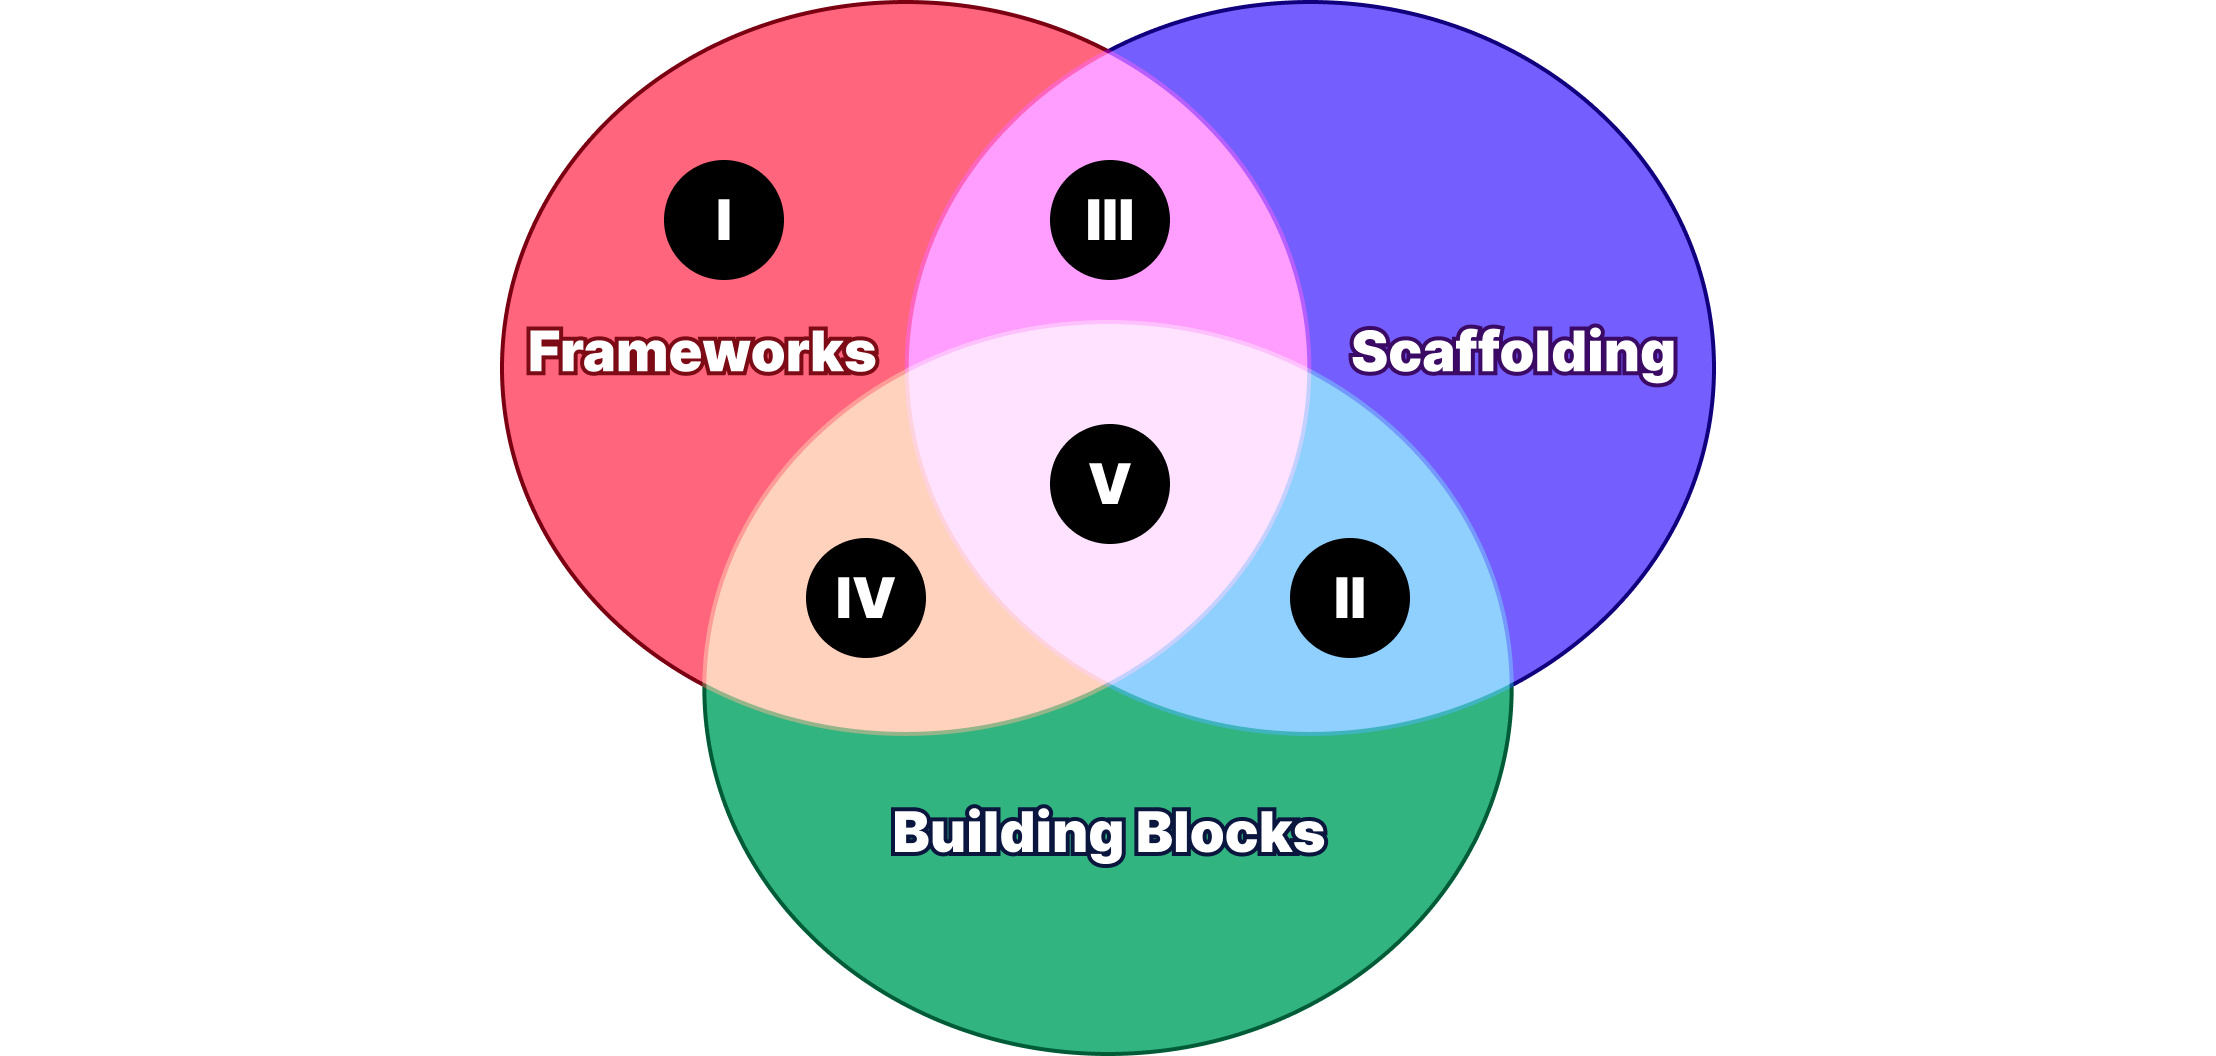
\includegraphics[width=\columnwidth, alt={A venn diagram of three circles, equally overlapping: frameworks, scaffolding, and building blocks. 5 Marks are made within the diagram, clarified in the caption.}]{figures/chapters.png}
%   \caption{%
%     The sections of this dissertation, with chapters marked. I) \textit{Chartability} is a framework. II) \textit{Data Navigator} is at the intersection of scaffolding and building blocks. III) \textit{Softerware} is at the intersection of frameworks and scaffolding. IV) \textit{Cross-perception} at the intersection of frameworks and building blocks. V) \textit{Skeleton} includes elements from all three.%
%   }
%   \label{fig:venn}
% \end{figure}

% # frameworks: tools that shape how we think, perceive, + design accessibility
% # scaffolding: tools that speed up and make more accessible, accessibility work
% # building blocks: tools that provide modular, and highly flexible materials for creating new experiences

The 4 domains of work that I engage in this thesis start first with \textbf{evaluation}. In work contexts where someone is designing and developing interactive data experiences, the practitioner must have the knowledge, tools, and resources available to systematically identify how their interfaces produce barriers for people with disabilities. A significant portion of professional accessibility work (arguably most, if not all) is founded on auditing and evaluating barriers to access. This work is pre-dominantly done through a standards-based approach~\cite{WCAG}, although in more robust evaluation work, people with disabilities are actively involved in the process~\cite{Power2012Guidelines}.

Evaluation is difficult work because much of it is contextually defined by the author themselves, and most tasks at this intersection require careful, non-automated processes and methods~\cite{Power2012Guidelines,Deque2021Automated}. To make matters more difficult, no comprehensive guidelines, tests, and tools exist in any singular location. Practitioners often must gather these resources themselves, which tend to be situated towards accessibility in general or are high-level and provide minimal usefulness in practice. Additionally, practitioners themselves often have little knowledge about the veracity or quality of any given bit of information they gather~\cite{Sharif2024Challenges,Joyner2022Wild}, and often do the work themselves to synthesize this disparate space of information into a usable format they can apply to their own evaluation work.

% The 3 tool types that I unpack in this thesis are not formal categorizations but rather categorized in a way that provides organization and support for the narrative of this dissertation. Additionally, as a meta-point to make, the structure of this dissertation, the artifact itself, is a hierarchy (with 3 parts, each with chapters, then with sections and subsections, and so on). And the pages of this artifact are read in a \textit{linear} fashion. But the ideal conceptual way to structure these categories is better suited with \textit{set theory} and visualized as a venn diagram (\Cref{fig:venn}). (This is a meta-point because \textit{Data Navigator} and \textit{Skeleton} explicitly focus on structuring data so that information can be meaningfully navigated in non-linear, non-hierarchical ways.)

% These 3 categories overlap, and most of my work falls within these overlaps. This non-dichotomous structure was intentional.

% In this thesis, I define \textbf{frameworks} as tools that shape thinking; they provide a \textit{frame} for orienting the practitioner, providing a reflexive artifact, a mirror, that helps the practitioner reflect on their own work, assumptions, and imagination. Frameworks matter because, ultimately, this dissertation seeks to study how tools shape the behavior of people who design, analyze, and develop using data. Frameworks, then, can become a powerful way to probe designer intentions, thoughts, and the qualities that comprise their work.

To engage this, our first main chapter focuses on \textit{Chartability}, a heuristic framework that enables designers, developers, and auditors to systematically evaluate data visualizations and interfaces for a wide range of accessibility barriers, considering people with visual, motor, vestibular, neurological, and cognitive disabilities. In this project, we did the hard work for other practitioners and contributed our collection of synthesized accessibility resources in a single workbook. We had practitioners try out our resource in real environments, in-situ, in order to learn more about the challenges and barriers they themselves faced in evaluation work. With \textit{Chartability}, practitioners, especially those with limited accessibility expertise, gained more confidence and clarity in assessing and improving their work. Additionally, \textit{Chartability} has since become widely applied as a framework that isn't just used for evaluation but also as design guidance in many contexts, internationally, including policy organizations, governmental groups, and more than 100 companies and businesses.

% The second category in this thesis are \textbf{scaffolding tools}, which I define as tools that enable faster, more efficient, more scalable construction. Scaffolding, in particular, structures a complex, technical \textit{system} that governs an authoring experience. Scaffolding for example may be a software package that aggregates many actions an author would take, providing a higher-level language or set of functionalities in fewer expressions. Scaffolding tools are important to study because they engage problems of \textit{scale} that arise in design and development work: what tensions are produced when systems must be made to suit everyone, including people whose access conflicts with another? Or what trade-offs exist when certain lower-level tasks either become automated or are left as manual points design of consideration?

\textit{Chartability} then opened up a significant landscape of new projects and research directions. From a combination of my existing expertise as a visualization designer and engineer, in addition to continued application of \textit{Chartability} in the wild, we began to identify the trickiest and most-difficult domains of work for practitioners. Chartability has 50 total heuristics, or tests, each organized under one of 7 principles. But 3 larger domains began to emerge as the areas where the most severe and dramatic accessibility barriers remained unaddressed: on data \textit{navigation}, analytical \textit{interaction}, and interface \textit{personalization}.

So the next section of this thesis engages the first of these three: \textbf{navigation}. Navigation is a fundamental type of interaction that is leveraged by modern software-based assistive technologies. Screen readers, the primary tool used by people who are blind to interact with computers, navigate content. Additionally, many other assistive technologies, such as a sip and puff device (like the ``POSSUM'' from as far back as '63~\cite{Maling1963}) also navigate. Navigational technologies are leveraged by people with a significant array of disabilities, yet tend to be entirely ignored by existing data visualization tools, which are pre-dominantly built to support direct input (using a computer mouse).

Empirical work has already demonstrated that structural navigation is actually good~\cite{Zong2022Rich}, even when regular alternative text (image descriptions) exist. This is both because people who are blind can gain both a high level understanding (from the description) as well as lower-level sense of the data's structure and arrangement, in addition to the fact that discrete, structural navigation exposes interactivity that may exist on any visualization elements (such as they can be hovered or clicked with a mouse in order to perform some action). So, if good empirical work exists: \textit{why haven't practitioners put this research into action? What makes this work hard to do?}

We first built \textit{Data Navigator} to provide the building blocks we needed in order to address the technical and conceptual gaps that were required to make any visualization or visualization tool provide a navigable, interactive structure. \textit{Data Navigator} is a low-level toolkit which can be used to construct accessible navigation structures such as lists, trees, and diagrams from an underlying graph structure. We leveraged graph theory for an applied HCI problem: nodes and edges represent any relationships within the data as a structure, which then supports rich expressiveness of data navigation experiences. Users can navigate discrete marks in a visualization, clusters, groupings, and more. In addition to its structural scaffolding, \textit{Data Navigator} also supports a wide array of input modalities leveraged by people with disabilities (screen readers, keyboards, speech, and gestures).

\textit{Data Navigator} provided a substrate, but this contribution alone wasn't enough to engage the question \textit{why is navigation so hard, in practice?}. So the chapter following \textit{Data Navigator} introduces \textit{Skeleton}, a data navigation authoring tool built on top of \textit{Data Navigator}. Our novel approach in \textit{Skeleton} involves visualizing and making manipulable the nodes, edges, and textual data that comprise non-visual end user experiences. \textit{Skeleton} visualizes the building blocks that comprise \textit{Data Navigator}. Additionally, \textit{Skeleton} provides expressive, rapid scaffolding capabilities that leverage data visualization rendering engines. This scaffolding engine helps practitioners quickly create common configurations for non-visual data navigation structures that retain visual congruence to the underlying structure.

But most importantly, \textit{Skeleton} serves as a framework that shapes designerly consideration. Our conjecture was that because sighted practitioners cannot \textit{see} navigation building blocks, they will not treat those elements as iterable design materials. We conjectured: Navigation is hard in practice because sighted designers face barriers to iteration and understanding. We conducted an empirical study with sighted practitioners and found that making non-visual elements visual helped practitioners shift from treating accessibility as a compliance task to treating it as a design problem, re-iterating on the visual aspects of their design, and engaging in the complex and nuanced components that comprise data navigation experiences.

% The final category of our work focuses on tools that are \textbf{building blocks}, which we define as tools that provide modular, highly flexible, specifiable materials. The goal of building blocks is providing expressiveness and possibility to data practitioners. \textit{Data Navigator} is also a building block type of tool, for enabling entirely novel structured experiences of data navigation. And building blocks matter as a point of study because \textit{possibility} is a space of rich design potential. Building blocks then can become a probe used to evoke and elucidate the imagination and consideration of practitioners thinking through problems and new ideas.

Now, \textbf{interaction} becomes the next area we wanted to engage. Existing accessible data interaction for people who are blind, including our previous work on navigation (which is a form of interaction), predominantly seeks to expose information. This is what we call \textit{access-oriented interaction}. In terms of low-level analytical tasks, most are then made feasible through navigation, sonification, or summarization-based and question-answering approaches: retrieving values, filtering, computing derived values, sorting, determining ranges, clustering, and finding outliers. What remains are analytical tasks that, despite being ``low level'' (understood as \textit{unable to be reduced into more fundamental tasks}), are cognitively highly complex: finding correlations and characterizing distributions~\cite{Amar2005}. These tasks require complex hypothesization and exploration, rather than a system that simply encourages surfacing what is known or what is already present in the data: it requires combining, remixing, restructuring, and dividing data.

But blind \textit{analytical interaction} isn't just important to engage because it is understudied, it is important to engage because many of interactive information visualization's most impactful tools for data science enable it~\cite{Flowers1997Cross,Weaver2008,Moritz2019,heer_mosaic_2023}. In visualization, \textit{cross-filtering} is one example of an interaction that enables a user to filter one visual space while seeing a coordinated change in another visual space simultaneously and near-instantaneously. The speed of input interaction and perception of output also matters: even a small bit of latency changes the quality of a user's data exploration activities~\cite{Liu2014}. We conjectured that a screen reader, the most-used tool leveraged by blind people when interacting with computers, may be insufficient for engaging this task.

To engage this, this thesis introduces \textit{Cross-perception}, an approach for building analytical interactions that support perception in one space of input interaction with simultaneous, non-competing perception of output in another space of data representation. We first formalized a design framework for producing \textit{cross-perception} experiences and then built a novel prototype device, the \textit{cross-feelter}, that enables blind \textit{cross-perception} of a cross-filtering data exploration interface. In an empirical study with blind users (with and without existing data expertise), we found \textit{cross-perception} speeds up analytical exploration by 90\% and helps blind users consider vastly more questions of their dataset (+188\% computational queries, +54\% spoken aloud) compared to a screen reader-driven interaction.

Beyond performance, we found that our input modality itself shaped the character of analytical engagement: participants didn't just work faster, they considered more dimensions of their data and asked qualitatively different questions. The \textit{cross-feelter} also reduced anxiety and substantially increased enjoyment, particularly for participants without prior data expertise, suggesting that the barriers blind practitioners face in data work are not only functional but affective. Additionally, we had our blind practitioners imagine new interaction possibilities that \textit{cross-perception} could enable including and beyond our \textit{cross-feelter} device.

Our final domain of work is the most difficult for visualization practitioners to engage: \textbf{personalization}. While \textit{navigation} demanded better software tooling and visual support and \textit{interaction} required new hardware, \textit{personalization} completely re-orients how software authoring takes place. Personalization matters because of \textit{access friction}, which is a design challenge where one design or interface configuration that might be accessible for one person or group of people turns out to create barriers for someone else~\cite{Hsueh, Hamraie}. In existing work on personalization and accessibility, studies have demonstrated that end-user control is great to have and can alleviate friction~\cite{Jones2024,Wood2023}, but little work has been done to explore what personalization looks like for an existing data visualization library and how practitioners should build and maintain their existing systems to support it.

Our final chapter introduces \textit{Softerware} to address the tension between standardized accessible design and the diverse needs of real users with disabilities. In the wild, \textit{access friction} exists in every design that reaches a public audience; it is inevitable. This tension ultimately means that some users have a worse experience, and may even face exclusion, with any particular design configuration. So for this work, we conducted our research in-situ with visualization software engineers and designers and worked to build a scalable, flexible software system dubbed ``softerware'' that enables end users to manipulate the appearance and functionality of the charts and graphs they encounter according to their own preferences. We conducted empirical research to inform our collaborators, as well as other visualization system authors, with guidelines and considerations for building \textit{softerware} systems. In our study, no two participants chose the same preference configuration and participants with the same diagnosed condition sometimes needed opposite design treatments. Practitioners, meanwhile, immediately raised ethical concerns about whether personalization would let designers off the hook for poor defaults. These findings revealed that the real barriers to personalization are not at the level of any individual chart but at the level of system infrastructure: without persistence, cross-system interoperability, and shared standards, the effort required of end users exceeds the value they receive.

Combined, these contributions provide empirical insights and practical advancements in the state of the art for tooling that bridges gaps in current accessibility practices in visualization and data science. Our work ultimately enables people with and without disabilities to better evaluate barriers in, analyze with, design for, develop, and personalize interactive data experiences. We demonstrate that tool-making is a productive intervention that both engages accessibility barriers and elucidates why those gaps exist in practitioner work.

% Together, these contributions provide both empirical insights and practical tools that bridge gaps in current accessibility practices, ultimately enabling practitioners to build richer, more inclusive data experiences for all users.

\part{Evaluation: Helping Practitioners Identify Accessibility Barriers}

\chapter{\textit{Chartability}: Heuristics as a Tool and Resource}

\noindent\rule{16cm}{0.4pt}
\begin{quote}
This chapter was adapted from my published paper:
\begin{adjustwidth}{1cm}{}
% \-\hspace{2cm}
F. Elavsky, C. Bennett, and D. Moritz, ‘How accessible is my visualization? Evaluating visualization accessibility with Chartability’, \textit{Computer Graphics Forum}, vol. 41, no. 3, pp. 57–70, Jun. 2022.
\end{adjustwidth}
\end{quote}
\noindent\rule{16cm}{0.4pt}

\section{Abstract}

Novices and experts have struggled to evaluate the accessibility of data visualizations because there are no common shared guidelines across environments, platforms, and contexts in which data visualizations are authored. Between non-specific standards bodies like WCAG, emerging research, and guidelines from specific communities of practice, it is hard to organize knowledge on how to evaluate accessible data visualizations. We present Chartability, a set of heuristics synthesized from these various sources which enables designers, developers, researchers, and auditors to evaluate data-driven visualizations and interfaces for visual, motor, vestibular, neurological, and cognitive accessibility. In this paper, we outline our process of making a set of heuristics and accessibility principles for Chartability and highlight key features in the auditing process. Working with participants on real projects, we found that data practitioners with a novice level of accessibility skills were more confident and found auditing to be easier after using Chartability. Expert accessibility practitioners were eager to integrate Chartability into their own work. Reflecting on Chartability’s development and the preliminary user evaluation, we discuss tradeoffs of open projects, working with high-risk evaluations like auditing projects in the wild, and challenge future research projects at the intersection of visualization and accessibility to consider the broad intersections of disabilities.

\section{Overview}

26\% of people in the United States self-report living with at least one disability~\cite{Okoro2018Prevalence}. Of those, 13.7\% live with a mobility disability and 10.8\% with a cognitive disability. Globally, the World Health Organization reports that 29\% of the world lives with uncorrected or uncorrectable blindness, low vision, or moderate to severe visual impairment~\cite{OrganizationWorld}. Access is a significant inclusion effort that has broad international impact, especially for data visualization. 

Accessibility is the practice of making information, content, and functionality fully available to and usable by people with disabilities. As part of this process, practitioners need to be able to identify accessibility barriers. While general accessibility standards help, evaluating the inaccessibility of complex data systems can be a daunting and often expensive task. State-of-the art automated compliance checkers only find 57\% of accessibility errors~\cite{Deque2021Automated}, meaning accessible experiences must still be manually designed and checked for quality. And following standards may only account for up to half of the needs of people with disabilities~\cite{Power2012Guidelines} anyway. Additionally, the intended wide applicability of these general standards means they fall short for information-rich systems, such as data visualizations (which use size, color, angles, shapes, and other dimensions to encode information). These specific contexts, communities, and libraries that deal with data visualizations and information-rich interfaces often have their own tools and guidelines for use, but they seldom include accessibility. Finally, research at the intersection of data visualization and accessibility has yet to meaningfully permeate data visualization tools and communities and primarily focuses on blindness and low vision, neglecting diverse accessibility needs of people with other disabilities.  

Synthesizing evolving accessibility standards, research findings, and artifacts from communities of practice into usable knowledge for a specific, evolving domain is a wicked problem. To address this, we present Chartability. Chartability is an accessibility evaluation system specific to data visualizations and interfaces which aims to help practitioners answer the question, ``how accessible is my data visualization?'' Chartability organizes knowledge from disparate bodies of work into testable heuristics based on the functional accessibility principles POUR (Perceivable, Operable, Understandable, and Robust)~\cite{InitiativePrinciples} and 3 novel principles CAF (Compromising, Assistive, and Flexible), which we added to attend to the unique qualities and demands of data visualizations. We refer to these 7 heuristic principles as POUR+CAF. Chartability is a community-contributed project that leverages the governance strategies of open source projects as a way to address the complex dual-evolution of both accessibility and data interaction practices. 

We additionally present an initial, light evaluation of Chartability from the experience of practitioners using it. We set out to see if using Chartability reduces the barrier of entry into this work for accessibility novices and if accessibility experts had any feedback to share about its use. We gave practitioners introductory material for Chartability and instructed them to use it according to their needs. We found that before using Chartability only accessibility experts believed auditing data visualizations to be somewhat easy or easy, while the other group believed auditing data visualizations to be somewhat hard or hard. All novice accessibility practitioners became more confident after using Chartability and believed auditing data visualizations for accessibility to be less difficult. Conversely while the expert accessibility practitioners were already confident in their ability to evaluate accessibility (and all unanimously had no change in their before and after evaluations), they were excited to adopt Chartability into their set of auditing resources. 

Our work sets out to acknowledge that data practitioners face significant barriers when first making data visualizations, systems, and experiences accessible. While Chartability contributes to filling gaps and organizing knowledge, it also challenges visualization and data interaction researchers to explore new horizons of possibilities in this space. As such, we conclude with recommendations for future research at the crossroads of data visualization and accessibility. 

\section{Existing Work in Data Visualization and Accessibility}

While recent works at the intersection of data visualization and accessibility are promising, they do not provide a consistent and unified methodology for designers to evaluate the accessibility of their work across the broad spectrum of disability considerations.

\subsection{Research Advancements in Data Visualization and Accessibility}
In parallel to Mack \ea's ``What do we mean by Accessibility Research?''~\cite{Mack2021What} when we asked ``What do we mean by data visualization accessibility research?'' we found that nearly all topics of study were vision-related. Largely, access issues other than vision that affect data visualization (such as cognitive/neurological, vestibular, and motor concerns) are almost entirely unserved in this research space. Kim \ea found that 56 papers have been published between 1999 and 2020 that focus on vision-related accessibility (not including color vision deficiency), with only 3 being published at a visualization venue (and only recently since 2018)~\cite{Kim2021Accessible}. Marriott \ea found that there is no research at all that engages motor accessibility~\cite{Marriott}. We have found 2 papers that engage cognitive/neurological disability in visualization and 1 student poster from IEEE Vis, which are all recent (specifically intellectual developmental disabilities~\cite{Wu2021Understanding} and seizure risk~\cite{South2020Generating,South2021Detecting}). We found no papers that engage vestibular accessibility, such as motion and animation-related accessibility. We also found that there is no research specific to low vision disabilities (not blindness or color vision deficiency) unless conflated with screen reader usage in data visualization. Blind and low vision people are often researched together, but in practice may use different assistive technologies (such as magnifiers and contrast enhancers) and have different interaction practices (such as a combination of sight, magnification, and screen reader use)~\cite{szpiro_2016}. 

Since the 1990s, the most prominent and active accessibility topic in visualization has been color vision deficiency~\cite{Chaparro2017Applications,Nunez2018Optimizing,Oliveira2013Towards,Lee2020Reaching,Martinez2021Methodology}. Research projects that explore tactile sensory substitutions have been a topic in computational sciences dating back to the 1983~\cite{Schiff1983}, with tactile sensory substitutions being used for maps and charts as far back as the 1830s~\cite{HaleExtensive}. Sonification used both in comparison to and alongside visualization and tactile methods for accessibility dates as far back as 1985~\cite{Mansur1985Sound,Flowers1997Cross,Brewster2002Visualization,mcgookin_soundbar_2006,Zhao2008Data,Cullen2019Co}. Some more recent work has explored robust screen reader data interaction techniques~\cite{Godfrey2018Accessible,Sorge2016Polyfilling}, screen reader user experiences with digital, 2-D spatial representations, including data visualizations~\cite{Schaadhardt2021Understanding,Sharif2021}, dug deeper into the semantic layers of effective chart descriptions~\cite{Lundgard2022Accessible}, and investigated how to better understand the role of sensory substitution~\cite{Chundury2022Towards}. Jung \ea offer guidance that expands beyond commonly cited literature that chart descriptions are preferably between 2 and 8 sentences long, written in plain language, and with consideration for the order of information and navigation~\cite{Jung2022Communicating}. We find all of this emerging work promising and foundational.

Despite this promising work emerging, we also want to acknowledge a spectrum of other work that exists at the intersection of accessibility and data visualization that does not serve the goals of our project. There is significant research that explores automatic or extracted textual descriptions~\cite{Choi2019Visualizing,Balaji2018Chart,Chen2019Neural,Chen2020Figure,Lai2020Automatic,Obeid2020Chart,Qian2021Generating,Sharif2018evoGraphs} and haptic graphs and tactile interfaces~\cite{Aldrich2008Talk,Bornschein2015Collaborative, Brown2012VizTouch,Butler2021Technology,Gallace2011To,Schiff1983,Jansen2015Opportunities,Jayant2007Automated,Lederman1986Perception,SchneiderConstructing,Shi2016Tickers,Baker2016Tactile}. These research projects produce artifacts that are high-cost for individual use, some are not robust enough to interpret complex visualizations effectively, and several have not included people with disabilities. Since our goal is to synthesize knowledge for practitioner accessibility work, we also acknowledge that some of these projects did not follow standards during their research project and in their output, such as using Web Content Accessibility Guidelines~\cite{WCAG} or The American Printing House for the Blind and Braille Authority of North America~\cite{BANA2010Guidelines}. All of these challenges are factors that limit the generalizability of these artifacts and knowledge for practitioner use~\cite{Lundgard2019Sociotechnical,Moraes2014Evaluating,Sharif2021}. We encourage work to continue at the intersection of accessibility and visualization, but stress the importance of practical, disability-led research that either builds on or explicitly challenges standards.

\subsection{Accessibility Practices in Data Visualization Tools and Libraries}
Our research goals are to find what is already being done in data visualization and accessibility and to see if we can enhance that activity. To this aim, our background investigation includes a broad and comprehensive exploration of the field of practitioner and non-academic artifacts.

Some open source and industry contributions have pushed data visualization and related accessibility efforts. Libraries like Highcharts~\cite{Highsoft} or Visa Chart Components (VCC)~\cite{VisaVisa} and tools like the Graphics Accelerator in SAS~\cite{SASSAS} have broad accessibility functionality built in, but their documentation is technically specific to their implementation. While these relatively accessible libraries and tools can be helpful for inspiration, their specific techniques and guidance materials are not easily transferrable to other environments or applications where data visualizations are created. Practitioners must reverse engineer and deconstruct many of the methods employed by these libraries, and with the exception of VCC (which is open source), this task requires significant effort, given their primarily closed-box nature. 

In common charting tools and libraries (apart from those already mentioned) accessibility engineering is often not present, limited in scope, or has only recently become an effort. More established visualization libraries like matplotlib, ggplot2, d3js, R-Shiny, and Plotly have left most accessibility efforts to developers, with varying levels of documentation and difficulty involved~\cite{Forum2018Are, Community2018Making, CanelonRevealing, Forum2019Datatables, Wheatcroft2020Making}. None of these major tools have a broad spectrum of accessibility options built in and documented.

Community contributors often must fight to make their tools and environments accessible (sometimes even against the design of the tools themselves) with little to no compensation for their contributions. For example, Tableau’s first accessible data table was built by a volunteer community member Toan Hong as an extension~\cite{Hoang2018TableauMagic}. Tableau users more broadly must resort to voting systems to gather attention to accessibility issues~\cite{DeMartiniTableau}. Semiotic’s accessibility features were added by community member Melanie Mazanec~\cite{MazanecSemiotic}. For Microsoft’s PowerBI, students have organized resources for how to make visualizations built with it more accessible~\cite{KleinPower} while non-profits like the City of San Francisco’s data team have had to build features like keyboard instructions from scratch~\cite{SanCOVID}. Mapbox GL JS is an example of a popular mapping library (over 400,000 weekly downloads)~\cite{MapboxMapbox} that has no built-in accessibility support by default. The accessibility module for Mapbox GL on GitHub was created and maintained by volunteers but has had less than 10 weeks of work with any activity invested since its first activity in late 2017~\cite{Mapbox2021Mapbox}. 

Many community-driven efforts are under-utilized, must be discovered outside of the primary environment’s ecosystem, have poor or no core, internal support, and are inconsistently and partially implemented. Accessibility is still an afterthought in data visualization and ad-hoc, specific solutions proposed have not led to widespread improvements.

\subsection{Accessibility in Practice, Broadly}
Accessibility in practice is largely motivated by standards work or assistive technology. We want to acknowledge that tactile and braille standards are robust~\cite{BANA2010Guidelines}, but have limited transferability to digital contexts currently. For example, whereas tactile graphics guidelines lend insight into information prioritization, layout, and fidelity, the assumption is they will be embossed onto paper or similar physical mediums~\cite{Bigham2010VizWiz,Lundgard2019Sociotechnical,Sharif2021}.

In digital contexts, the most influential body for accessibility is the World Wide Web Consortium’s (W3C) Web Accessibility Initiative (WAI). WAI’s Web Content Accessibility Guidelines (WCAG)~\cite{WCAG} influence accessible technology policy and law for more than 55\% of the world’s population~\cite{Initiative2021Web}. WAI and WCAG outline 4 types of functional accessibility principles: Perceivable, Operable, Understandable, and Robust, abbreviated as POUR~\cite{InitiativePrinciples}. POUR is the foundation that organizes all 78 accessibility testing criteria in WCAG.

\subsection{Using Heuristics to Break Into Under-addressed Areas}
To summarize the complex problem space to which this paper contributes: Research in data visualization primarily focuses on visual accessibility, accessibility standards focus on a broad range of disabilities but lack deep contextualization for data visualization, and practitioners seem to build a wide array of solutions to fill these gaps, most of which are poorly maintained or adopted. Any time a practitioner wants to embark on a journey learning how to evaluate the accessibility of a data visualization, they must collect and synthesize this complex space of knowledge themselves. We have included (with permission) an exemplary field artifact as an example of this type of labor in our supplemental materials, which contributed to the United States Government's project, ``Improving Accessibility in Data Visualizations''~\cite{USImproving,USData}.

After gathering information with this breadth and complexity, a heuristic evaluation model was chosen as a way to deliver useful but flexible knowledge. Heuristic evaluation models have a long history in HCI and are cheap to use and require little expertise. They have been shown to be effective methods for practitioners compared to user testing, focus groups, or other evaluative methods that require existing expert knowledge or recruitment, moderation, and compensation of participants~\cite{Martinez2021Methodology,Chuan2015Usability,Brangier2018Beyond,Nielsen10,Joyce2016Mobile,Nielsen1994Heuristic,Otey2017methodology,Santos2018Heuristic,Slavkovic1999Novice,Boudreau2018Unlocking}. Heuristics are also not new in visualization~\cite{Forsell2010heuristic,Craft2005Beyond,Oliveira2017Adapting, Scholtz2011Developing} even among topics related to accessibility (color vision deficiency, specifically)~\cite{Santos2018Heuristic, Oliveira2013Towards}.

\section{Making Chartability}
We next present Elavsky’s work to develop Chartability as a real-world design process contribution to the larger research community. Our making process does not neatly fit into most design models that divide researchers from practitioners. In Gray's different models of practitioner-researcher relations, our work is some variation of bubble-up, practitioner-led research~\cite{Gray2014Reprioritizing}. This project was initiated by Elavsky while they were an industry practitioner, deeply situated in this work already.

Thus, the following description of Chartability’s 10-month creation is written from Elavsky’s perspective. The supplemental materials include the data from this stage of the process, a preview of which is available in \autoref{tab:table}: 
\begin{enumerate}
    \item \textbf{Situate, Survey, and Select Problem Space}: I was situated within the context of accessibility evaluations of data visualizations. From personal experience, I recognized the prohibitively significant labor involved in ensuring I was effectively following accessibility standards while also attending to the complex design considerations of data visualizations. To improve this work both for myself and others in the future, I surveyed existing problems and challenges others faced and selected a solution that I felt equipped to address.
    \item \textbf{Collect Existing Resources}: I set out to answer, ``If evaluating the accessibility of data experiences is hard, what do existing standards miss?'' I evaluated my seed knowledge (WCAG criteria) for shortcomings and gaps and collected other data relevant to my goal (academic and industry research, open-source libraries, tools, applications, data products, government guidelines, design guidelines, software documentation, university coursework, and practitioner articles).  
    \item \textbf{Code Resources}: After collating these resources (including relevant WCAG criteria), I loosely borrowed from thematic analysis~\cite{Braun2006Using} and qualitatively coded this data. I developed a set of 29 codes starting with WCAG's POUR principles and expanded the codes to account for other concerns that came up in the resources, including what type of accessibility was being addressed (e.g., cognitive, visual), whether a solution was technology-specific or agnostic, and other categories (like ``time-consuming'' or ``user-controlled''). I then divided the resources into codable segments with relatively distinct pieces of information and applied the 29 codes to the information segments. I grouped information with codes in common, resulting in a representative 45 groups of related information segments. 
    \item \textbf{Synthesize Heuristics}: Since auditing depends on measurable heuristics, I adjusted each of the 45 groupings that resulted from the qualitative analysis into phrasing that could be verified by an evaluation. I then augmented each heuristic with known testing procedures, resources, and tools necessary for applying them in practice. 10 critical heuristics (these were determined top priorities through user feedback) are previewed in \autoref{tab:table}, with the full version of this table (and more) provided in our supplemental materials.
    \item \textbf{Group Heuristics into Higher-level Principles}: I linked each heuristic with relevant web accessibility standards and POUR principles to draw a familiar connection for users who might already be accessibility practitioners. 26 heuristics fit neatly back into Perceivable, Operable, Understandable, or Robust.
    \item \textbf{Develop Remaining Themes into New Principles}: 19 remaining heuristics with complex codes and overlapping groups demanded new theorizing, as they either did not fit into POUR at all or could arguably belong to multiple principles at once. I analyzed these remaining complex heuristics and for similarities and organized them under 3 new themes, which we are contributing as new accessibility principles, Compromising, Assistive, and Flexible, defined below.
\end{enumerate}

\begin{table}[h]
  \caption{Previewing Chartability's 10 Critical Heuristics\\\hspace{\textwidth}\\\hspace{\textwidth}(Coding Categories are broken into two sections: first which POUR principles contributed to the heuristic while ``Other'' refers to how many additional coding categories were assigned.)}
  \label{tab:table}
  % \scriptsize
\begin{tabular}{lll|ll}
                &             &          & \multicolumn{2}{l}{Coding Categories} \\
  Heuristic Title & Principle   & Origin   & POUR              & Other           \\
  % \midrule
  Low contrast                             & Perceivable & Standard & P & 2 \\
  Small text                               & Perceivable & Research & P & 2 \\
  Content is only visual                   & Perceivable & Standard & P, R & 3 \\
  Interaction has only one input           & Operable & Standard & O, R & 3 \\
  No interaction cues/instructions         & Operable & Standard & O, U & 2 \\
  No explanation for how to read           & Understandable & Research & U & 1 \\
  No title, summary, or caption            & Understandable & Research & U & 1 \\
  No table                                 & Compromising & Research & O, U, R & 3 \\
  Data density inappropriate               & Assistive & Research & P, U & 4 \\
  User style change not respected          & Flexible & Standard & P, O, R & 6 \\
  ... +35 non-Critical heuristics          &  &  &  &  \\
\end{tabular}
\end{table}

\subsection{Compromising}
Compromising is a principle that focuses on Understandable, yet Robust heuristics. These heuristics are based on providing alternative, transparent, tolerant, information flows with consideration for different ways that users of assistive technologies and users with disabilities need to consume information. 

Compromising challenges designs that only allow access to information through limited or few interfaces or processes. These heuristics focus on providing information at a low and high level (such as tables and summaries), transparency about the state of complex interactions, error tolerance, and that data structures can be navigated according to their presentation. Compromising designs have both information and system redundancies in place. 

\subsection{Assistive}
Assistive is a principle that primarily builds off the intersection of Understandable and Perceivable principles but focuses on the labor involved in access. These heuristics include categories that encourage data interfaces to be intelligent and multi-sensory in a way that reduces the cognitive and functional labor required of the user as much as possible. 

The Assistive principle focuses on what Swan \ea refer to as ``adding value''~\cite{SwanInclusive} and what Doug Schepers meant by ``data visualization is an assistive technology''~\cite{SchepersWhy}. We visualize because it is faster and more efficient than munging cell at a time through data. Assistive heuristics ensure that both visual and non-visual data representations add value for people with disabilities. 

\subsection{Flexible}
Contrasted with Compromising (which focuses on robust understanding), flexible heuristics focus on robust user agency and the ability to adjust the Perceivable and Operable traits of a data experience. Flexible heuristics all have a tight coupling between a data experience and the larger technological context the user inhabits. The preferences that a user sets in lower-level systems must be respected in higher level environments. 

Self-advocacy and interdependent agency are important sociotechnical considerations that engage the conflicting access needs that different users might have in complex technological interactions like data experiences~\cite{Bennett2018Interdependence, Mankoff2010Disability}. Some users might want specific controls or presentation, while others might want something else entirely. Designs must not be rigid in their opinions and ability assumptions and should be designed to be moldable by and adaptive to user needs~\cite{Wobbrock2011Ability, Ladner2015Design}. 

\section{Using Chartability}

All of Chartability's tests are performed using Chartability's workbook~\cite{noauthor_chartability_nodate} alongside various tools and software (linked in the workbook). For the scope of this paper, we are not including an explanation for how to perform all of these. Both the workbook and supplementary materials with this paper give more details. 

While a highly trained auditor may be able to casually evaluate an artifact in as little as 30 minutes or even hold heuristics in mind as they are doing their own creative work, those new to auditing may take anywhere between 2 and 8 hours to complete a full pass of Chartability. Professional audits, which can take weeks or months, often include multiple auditors and provide rigorous documentation and detailed recommendations for remediation, typically in the form of a report. Chartability is meant to serve both quick pass and deep dive styles of audits, so users are expected to leverage it as they see fit. 

Below we give an example of what might be a quick pass audit, using Chartability. Which principles are applied in each of these stages are listed in parentheses in each heading. 

\subsection{Visual Testing (Perceivable)}

\begin{figure}
    \centering
    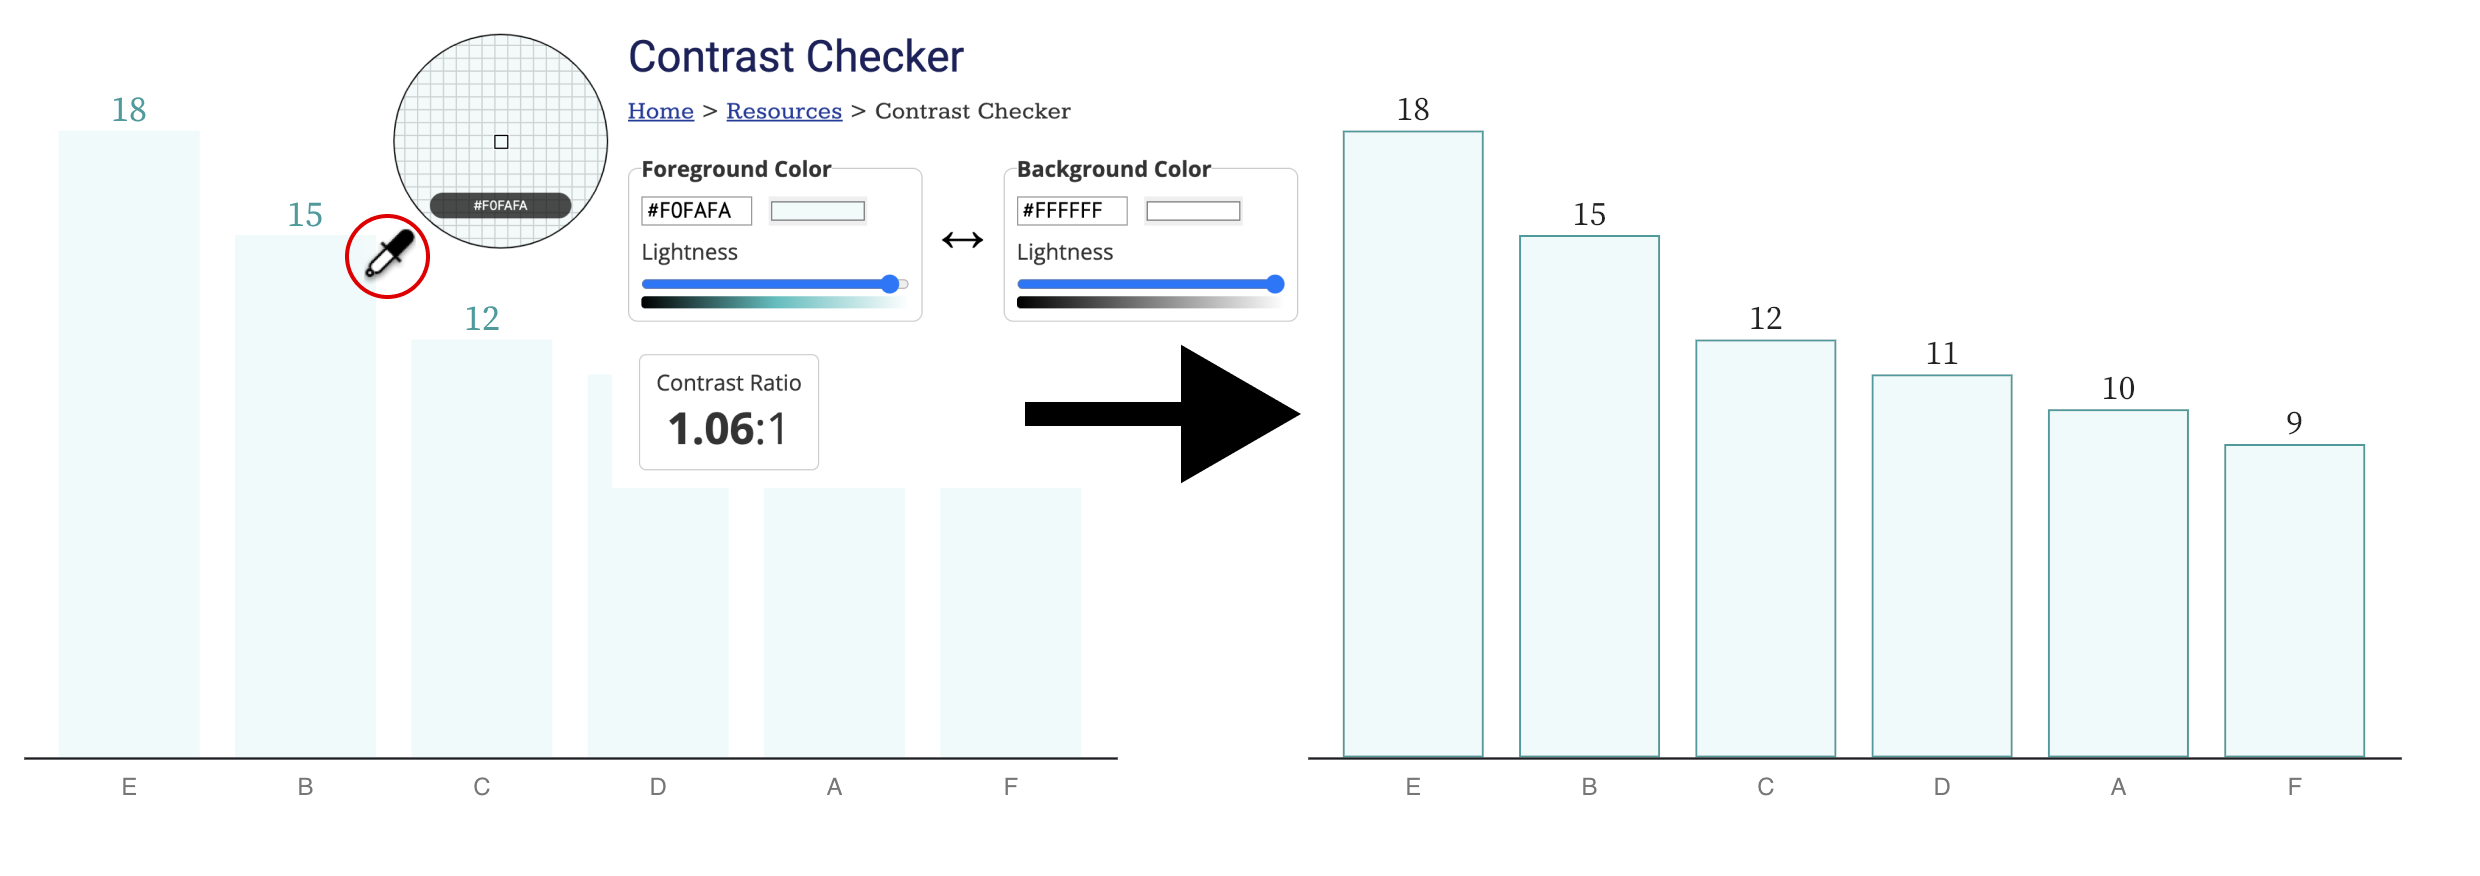
\includegraphics[width=0.75\linewidth]{figures/figure 2.png}
    \caption{A low contrast chart (left) compared to a higher contrast version (right). A dropper tool is extracting the fill color of the bar and then a contrast ratio has been calculated. Note that the fill color is the same on both bars, but darker borders have been added to ensure the visualization passes contrast tests.}
    \label{fig:2}
\end{figure}

Checking for contrast is the most common critical failure; 87.5\% of tests (7 out of 8) from our user study involving this heuristic failed, which supports the WebAim Million Report’s findings (83.9\% of the top 1 million websites also fail contrast testing, more than any other WCAG criteria)~\cite{WebAIMWebAIM}. In order to evaluate contrast, often a combination of automatic (code-driven) and manual tooling is performed. When manually auditing, practitioners typically use a dropper and a contrast calculator (\autoref{fig:2}). Most auditors find this to be one of the easiest tasks to perform and accomplishes 3 different heuristics in Chartability: ensuring text/geometries have contrast, interactive states for elements have enough contrast change, and the keyboard focus indicator is easy to distinguish. 

Perceivable heuristics also include tests and tools for color vision deficiency and ensuring that color alone isn't used to communicate meaning (like the redundantly encoded textures in \autoref{fig:9}). And another common, critical failure from Perceivable is text size. No text should be smaller than 12px/9pt in size.

\begin{figure}
    \centering
    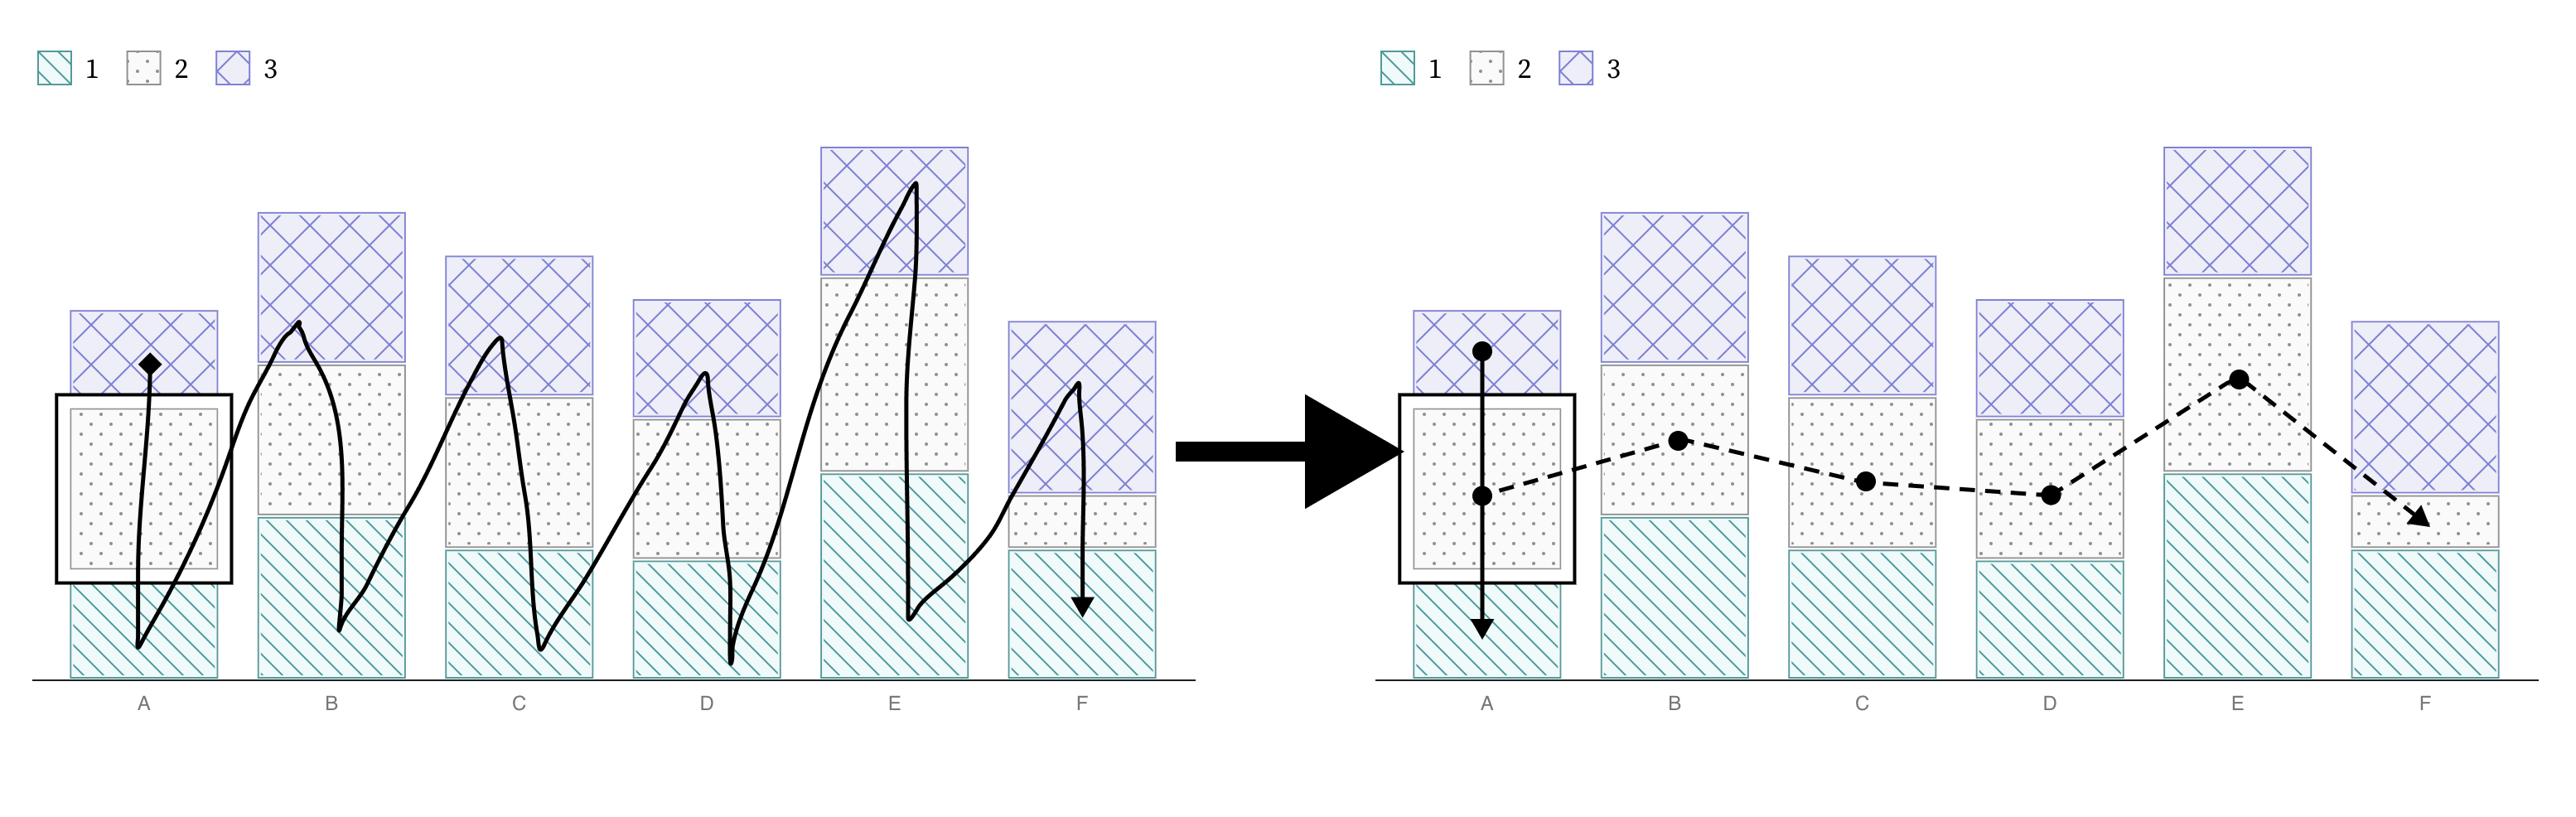
\includegraphics[width=0.75\linewidth]{figures/figure 3.png}
    \caption{Keyboard navigation paths on a stacked bar chart. The left shows a serial navigation example, typically just a default of rendering order. The right shows both groups (the stack of bars) and categories (the color/texture shared among bars across stacks) as dimensions to explore laterally or vertically.}
    \label{fig:3}
\end{figure}

\subsection{Keyboard Probing (Operable, Assistive)}
The next practice that most auditors should become comfortable with is using a keyboard to navigate and operate any functionality that is provided. Most assistive technologies, from screen readers to a variety of input devices (like switches, joysticks, sip and puffs, etc) use the keyboard api (or keyboard interface) to navigate content. If a data interface contains interactive elements (\autoref{fig:3}, \autoref{fig:4}), those elements (or their functionality) must be able to be reached and controlled using a keyboard alone. Auditors should be critical of how much work is involved in keyboard navigation, especially (\autoref{fig:8}). All that is required to start is the auditor begins pressing the tab key to see if anything interactive comes into focus. Arrow keys, spacebar, enter, and escape may be used in some contexts. Generally, instructions or cues should always be provided.

Using a keyboard provides an opportunity to evaluate many different heuristics: checking for multiple inputs (\autoref{fig:4}), whether the data structure that is rendered is navigable according to its structure (\autoref{fig:3}), and whether keyboard navigability across all elements in a data interface is even necessary (\autoref{fig:8}).

\begin{figure}
    \centering
    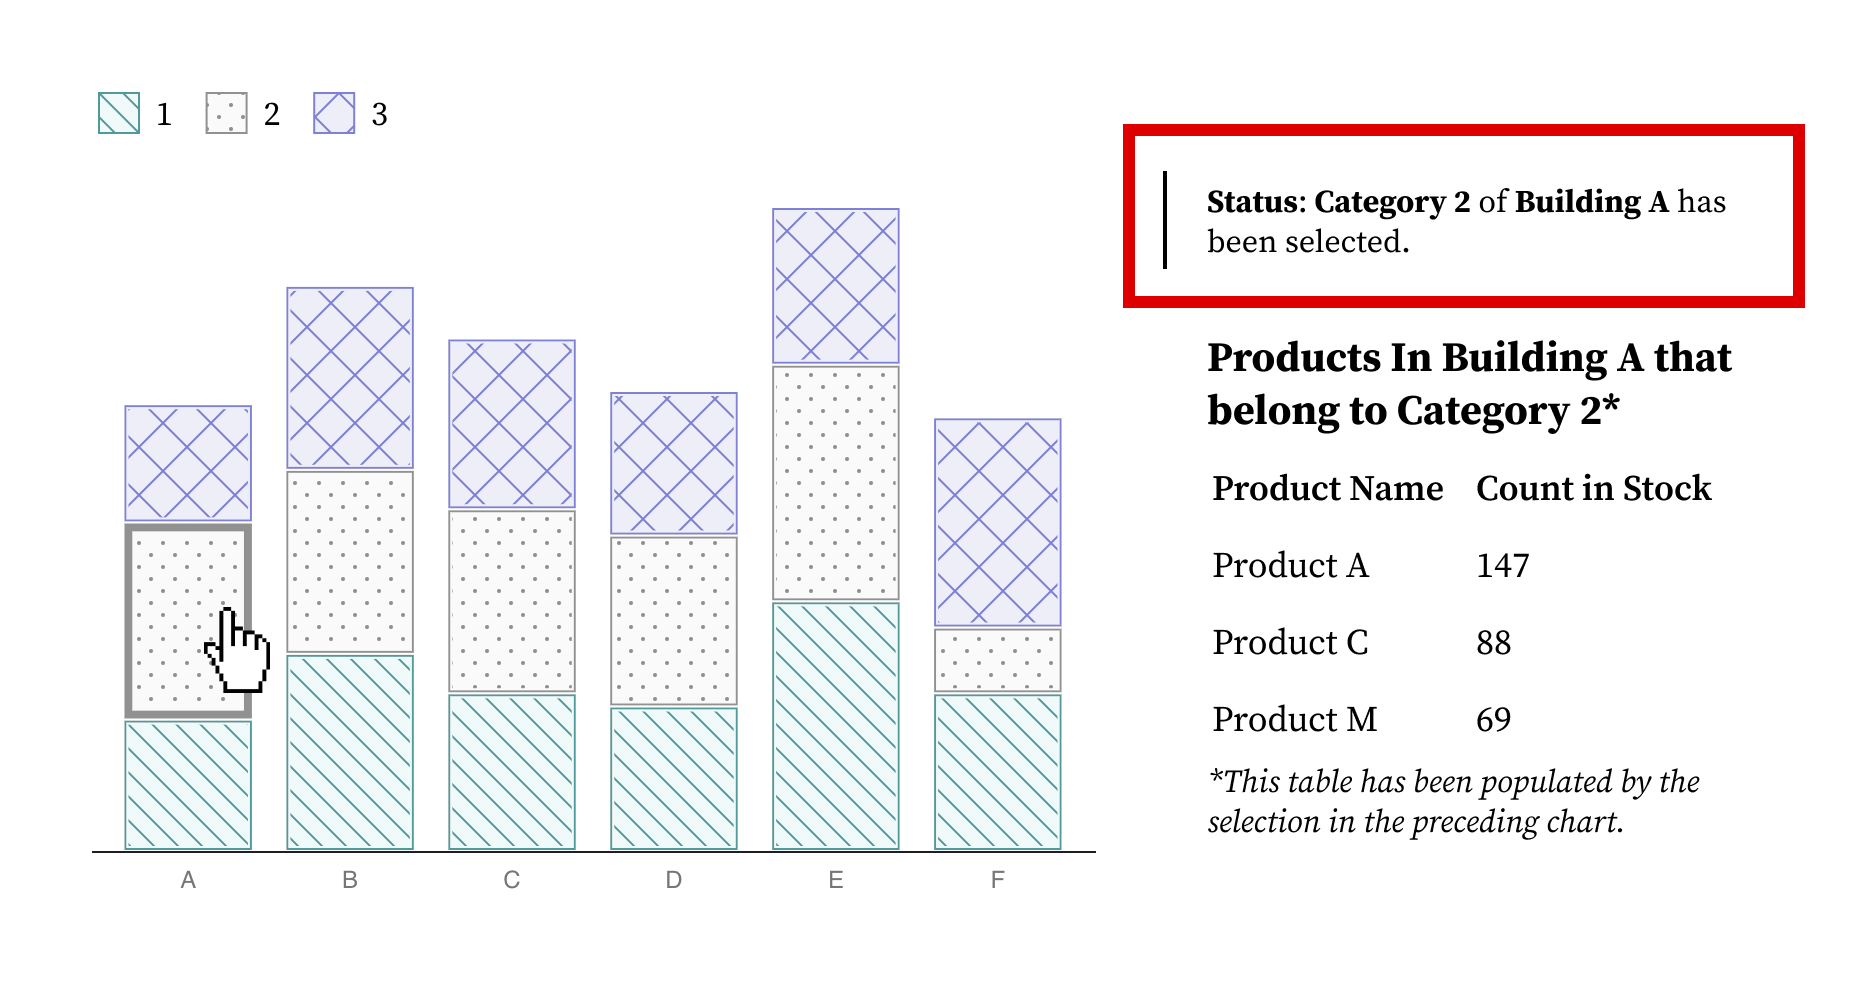
\includegraphics[width=0.75\linewidth]{figures/figure 4.png}
    \caption{A mouse cursor is selecting a bar (left, shown with a thick indication border) in a stacked bar chart to filter a dataset (on the right). A system alert (red box) notifies the user of their interaction result. This selection capability must also be provided for the keyboard interface and the alert must be announced to screen readers.}
    \label{fig:4}
\end{figure}

\subsection{Screen Reader Inspecting (Perceivable, Operable, Robust, Assistive) }
Closely related to keyboard testing is testing with a screen reader. Some things may work with a screen reader that do not with a keyboard (and vice versa), so both must be evaluated.

Screen readers, unlike more basic keyboard input devices, read out content that is textual (including non-visual textual information like \emph{alternative text}). Using a screen reader to audit is generally the hardest skill to learn. Keeping this in mind, testing whether the meaningful text provided in a visual (such as in \autoref{fig:5}) is accessible with a screen reader is the easiest and most basic test that auditors should first perform.

Next, all valuable information and functionality in a data experience should be tested whether it is available to a screen reader. This includes the individual variables about a mark as well as whether that mark is interactive (\autoref{fig:6}), whether status updates that reflect context change provide alerts (\autoref{fig:4}), and whether summary textual information is provided about the whole chart (\autoref{fig:5}) as well as statistically and visually important areas of that chart (\autoref{fig:8}). 

\begin{figure}
    \centering
    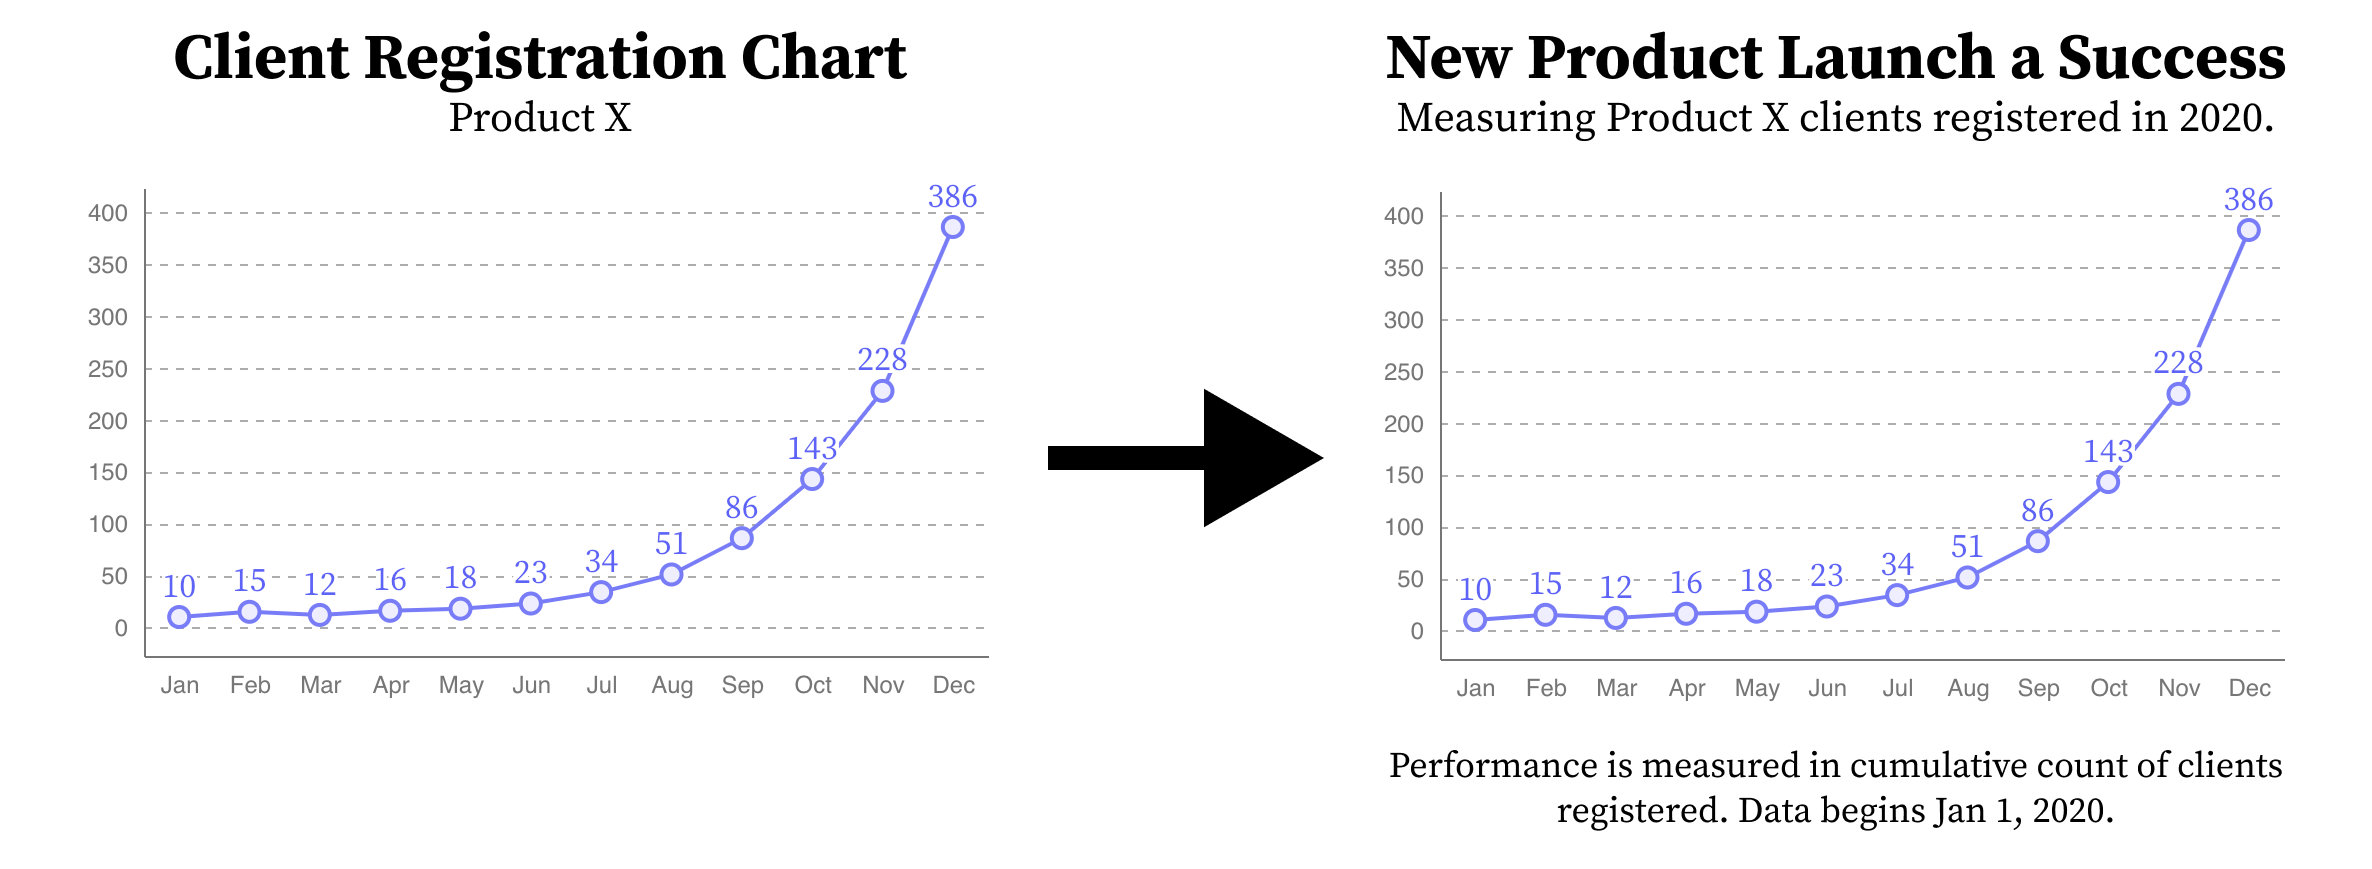
\includegraphics[width=0.65\linewidth]{figures/figure 5.png}
    \caption{Charts must have a visually available textual explanation provided that summarizes the outcome. ``Client Registration Chart'' for ``Product X'' (left) is inaccessible while ``New Product Launch a Success'' (right) gives a clear takeaway.}
    \label{fig:5}
\end{figure}

\begin{figure}
    \centering
    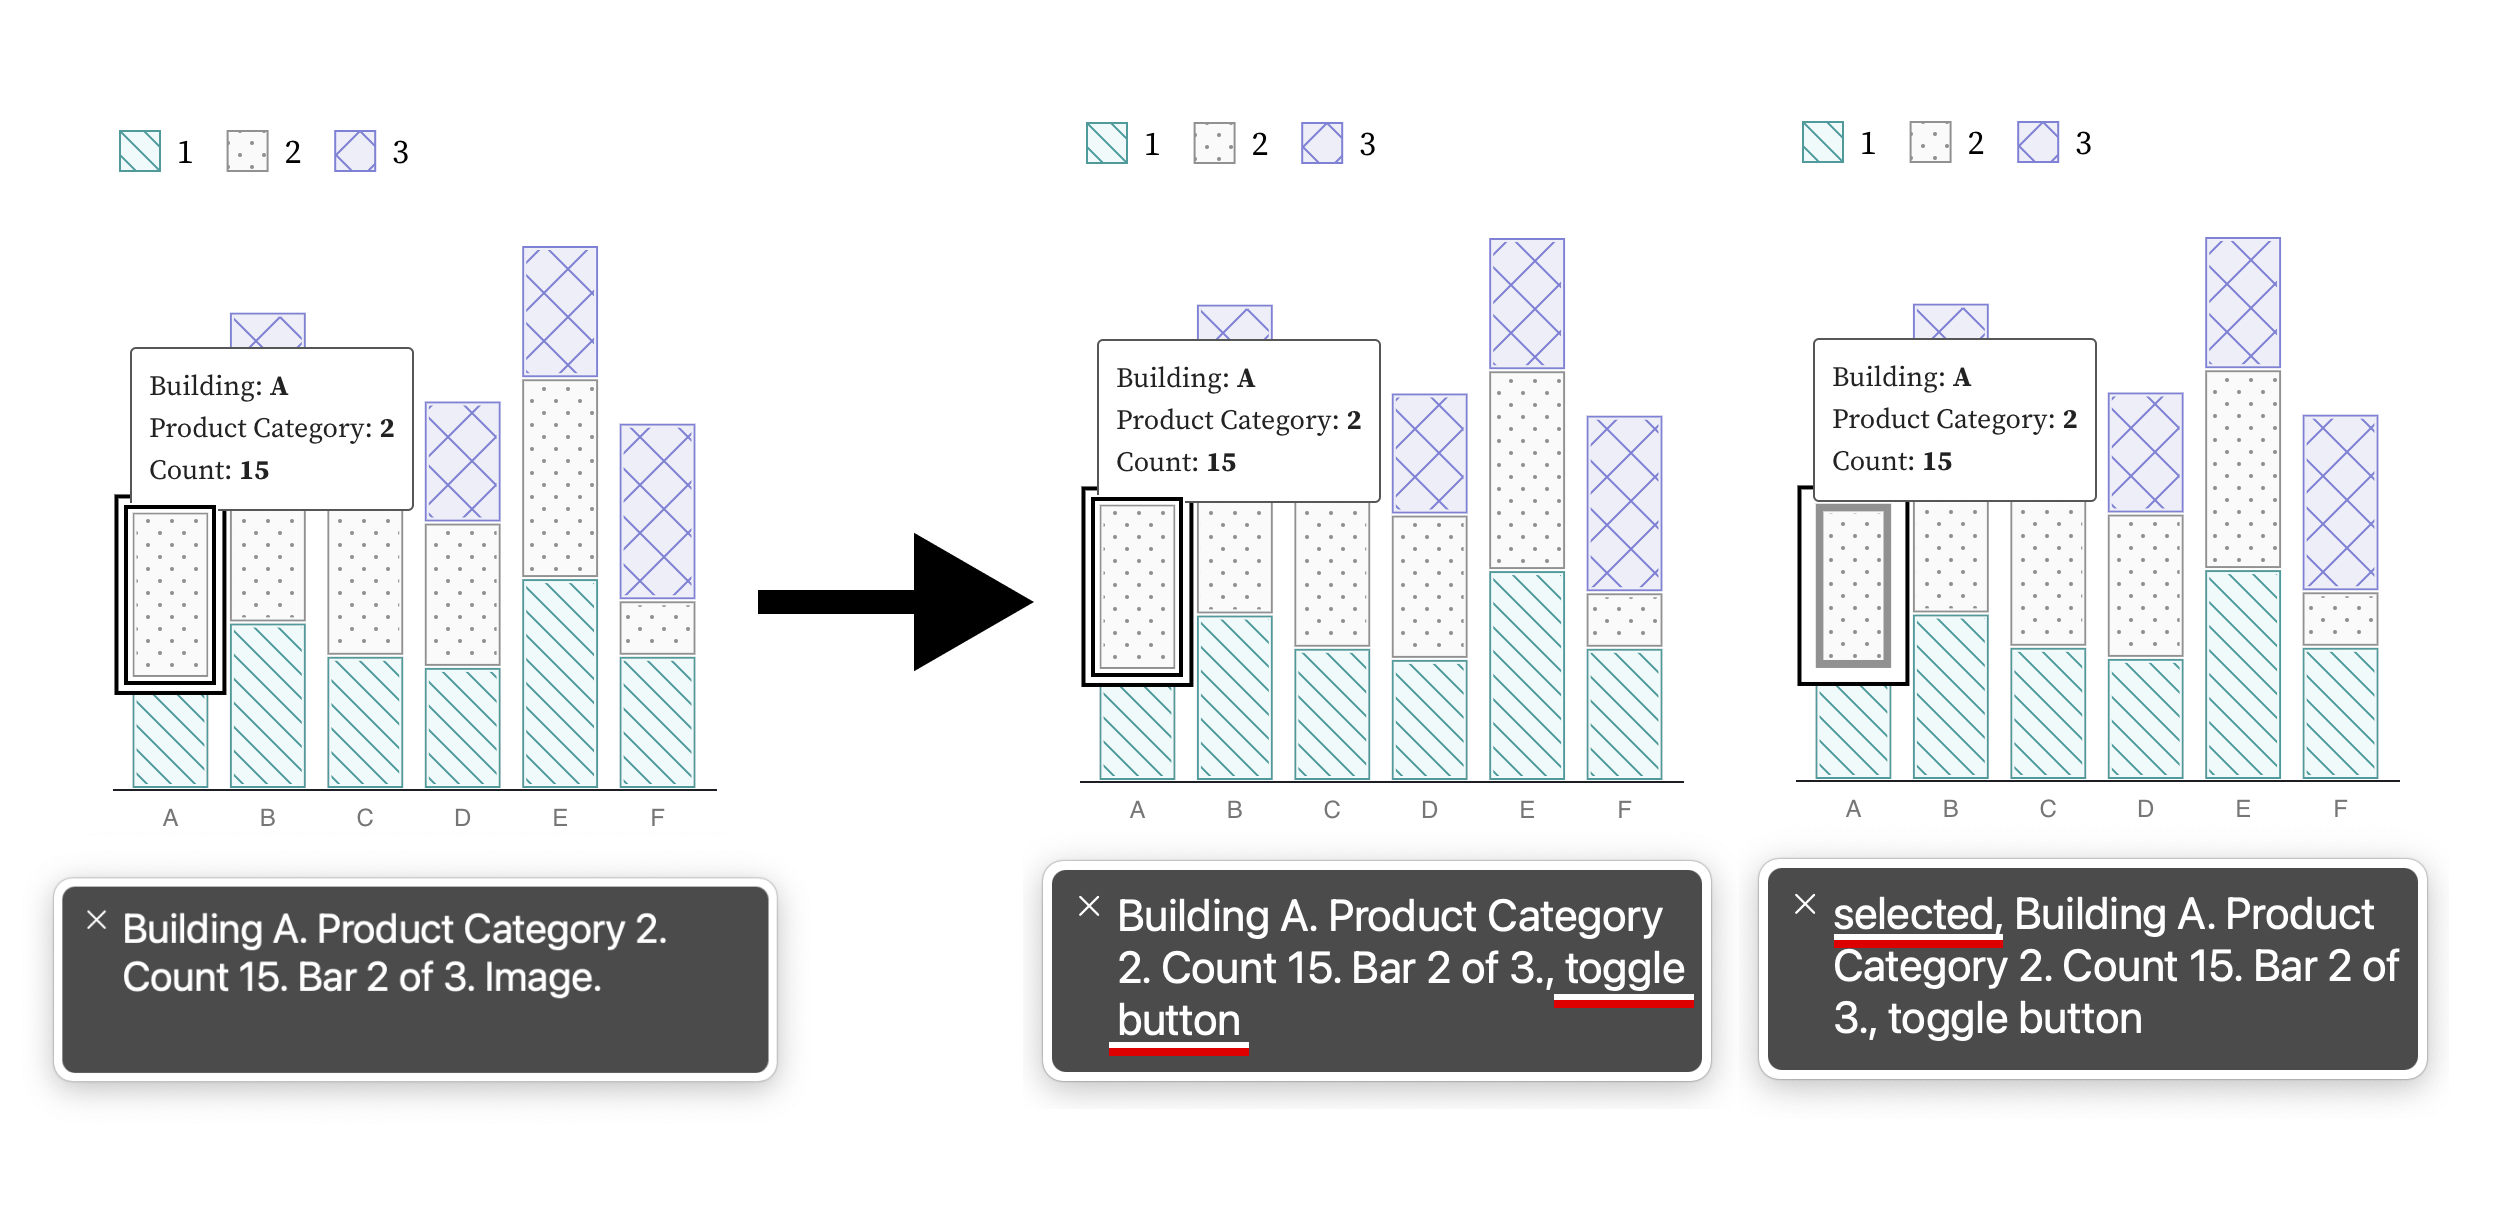
\includegraphics[width=0.65\linewidth]{figures/figure 6.png}
    \caption{An interactive chart displaying only ``Image'' as semantic information with no feedback provided on selection. The robust semantics given to a screen reader, ``toggle button'' (middle) as well instant feedback, ``selected'' (right) are considered proper semantics for an interactive experience.}
    \label{fig:6}
\end{figure}

\begin{figure}
    \centering
    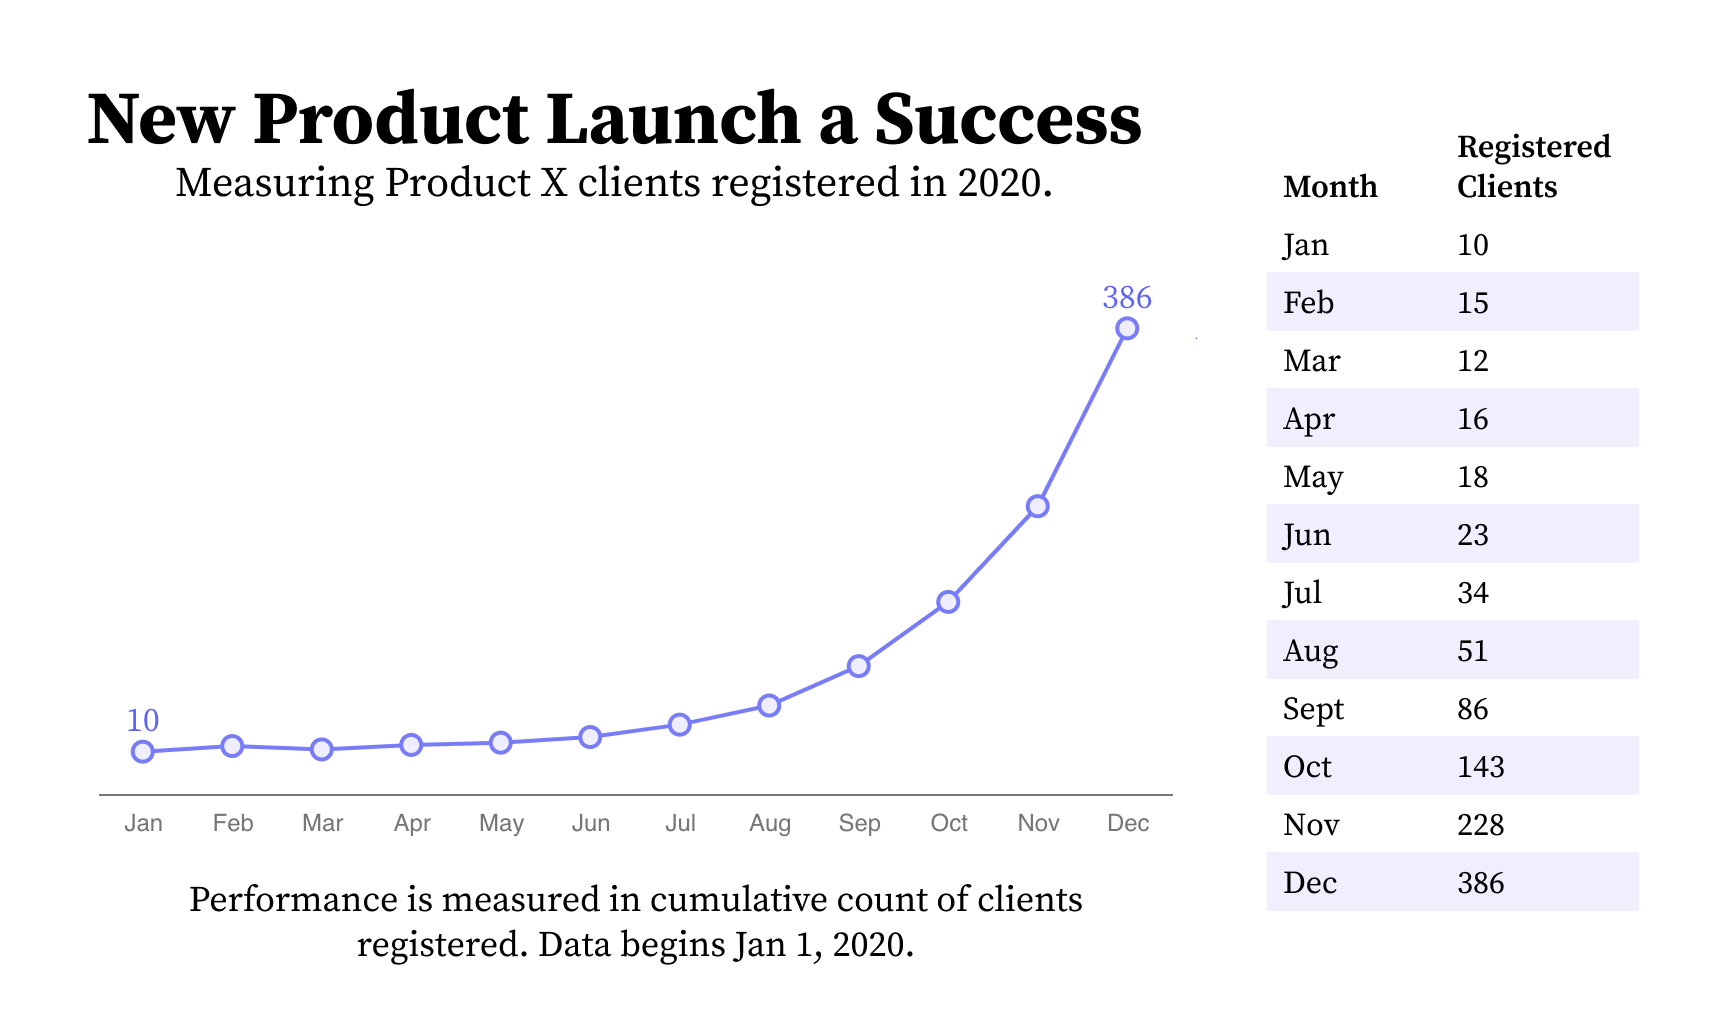
\includegraphics[width=0.5\linewidth]{figures/figure 7.png}
    \caption{A line chart (left) with a single line and an accompanying data table (right). This line chart would not provide enough low-level information about each datapoint without the table provided. A table alone however would also be inaccessible. Providing both can satisfy conflicting accessibility needs for different audiences.}
    \label{fig:7}
\end{figure}

\subsection{Checking Cognitive Barriers (Understandable, Compromising)}
First, auditing for cognitive barriers generally involves checking the reading level and clarity of all available text using analytical tools. But Chartability also requires that all charts have basic text that provides a visually-available textual description and takeaway (\autoref{fig:5}). This alone is one of the most important things to check for. In complex cases where a chart has a visual feature with an assumedly obvious takeaway, checking for annotations or textual callouts is important to help avoid interpretive issues~\cite{Xiong2020Curse} (\autoref{fig:8}).

\begin{figure}
    \centering
    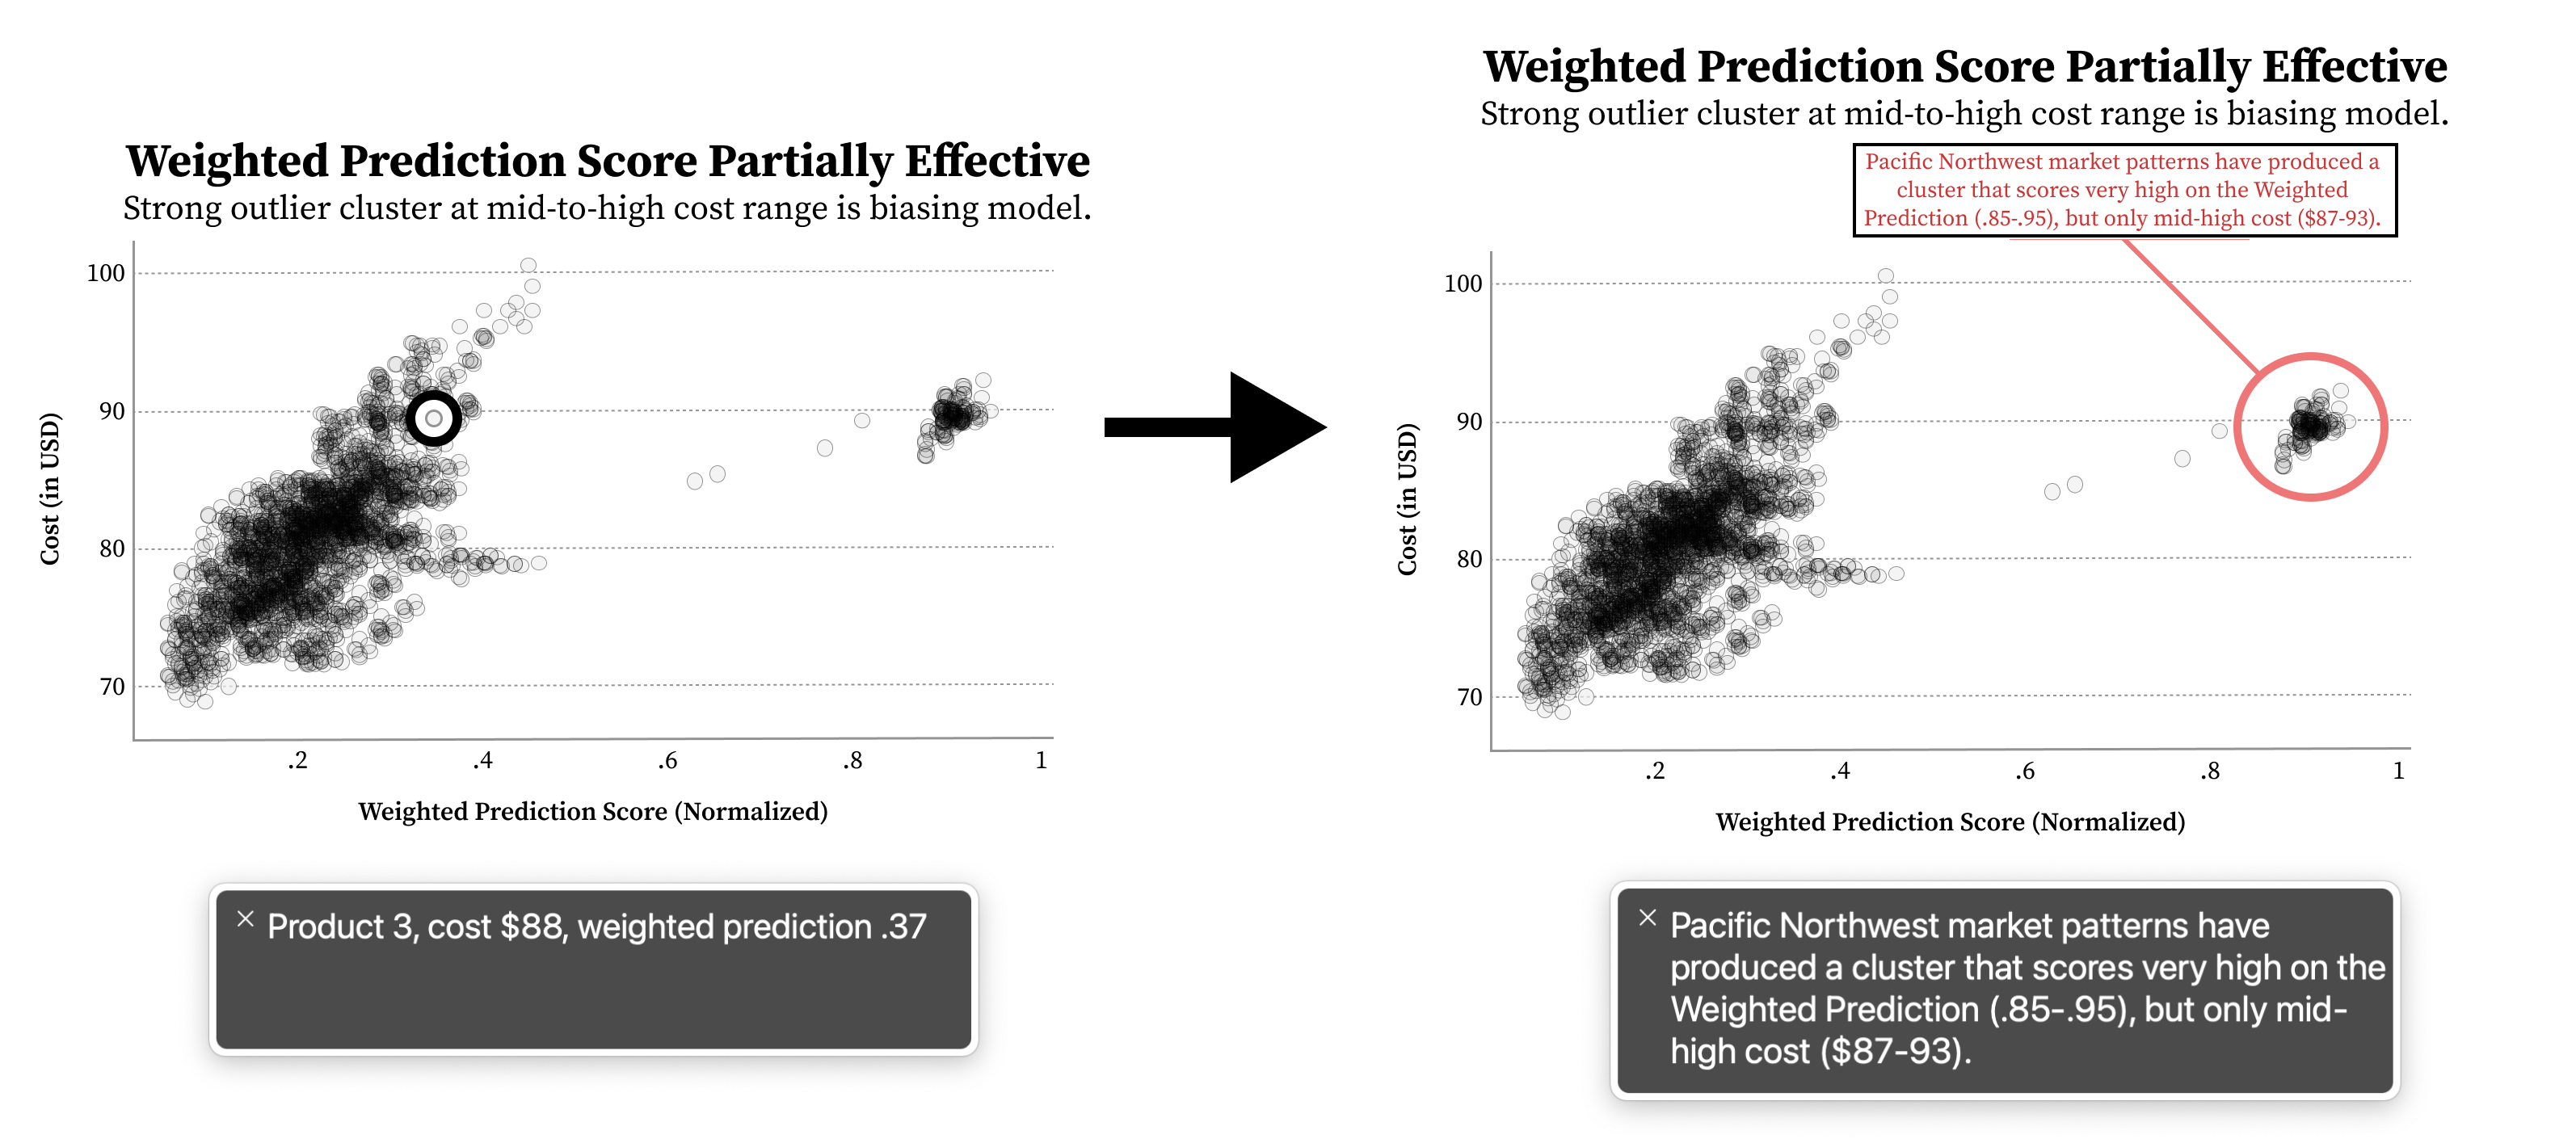
\includegraphics[width=0.75\linewidth]{figures/figure 8.png}
    \caption{A scatterplot with many points, where a single point within the chart can be accessed by a screen reader (left). Navigating this data piece by piece is unnecessarily tedious, so an annotation callout is provided to help the reader focus on an outlier cluster (right). The callout is being accessed by a screen reader, which is displaying the annotation’s summary as well.}
    \label{fig:8}
\end{figure}

\subsection{Evaluating Context (Robust, Assistive, Flexible) }
The final series of checks an auditor should make involve thinking about the overall work in a design (as it intersects with other considerations) as well as the larger technical context where the user is situated.

Auditors should first try to change system settings (such as toggling high contrast modes) to see whether a data experience respects these settings (\autoref{fig:9}), run automatic semantic evaluations as well as manually check for appropriate meaning (\autoref{fig:6}), and check if dense or highly complex visuals have sonified, tactile, or textual summaries available (\autoref{fig:8}). Auditors should also check whether system updates provide clear feedback textually (\autoref{fig:4}) as well as checking if there are both high and low level representations of information available (\autoref{fig:7}).

\begin{figure}
    \centering
    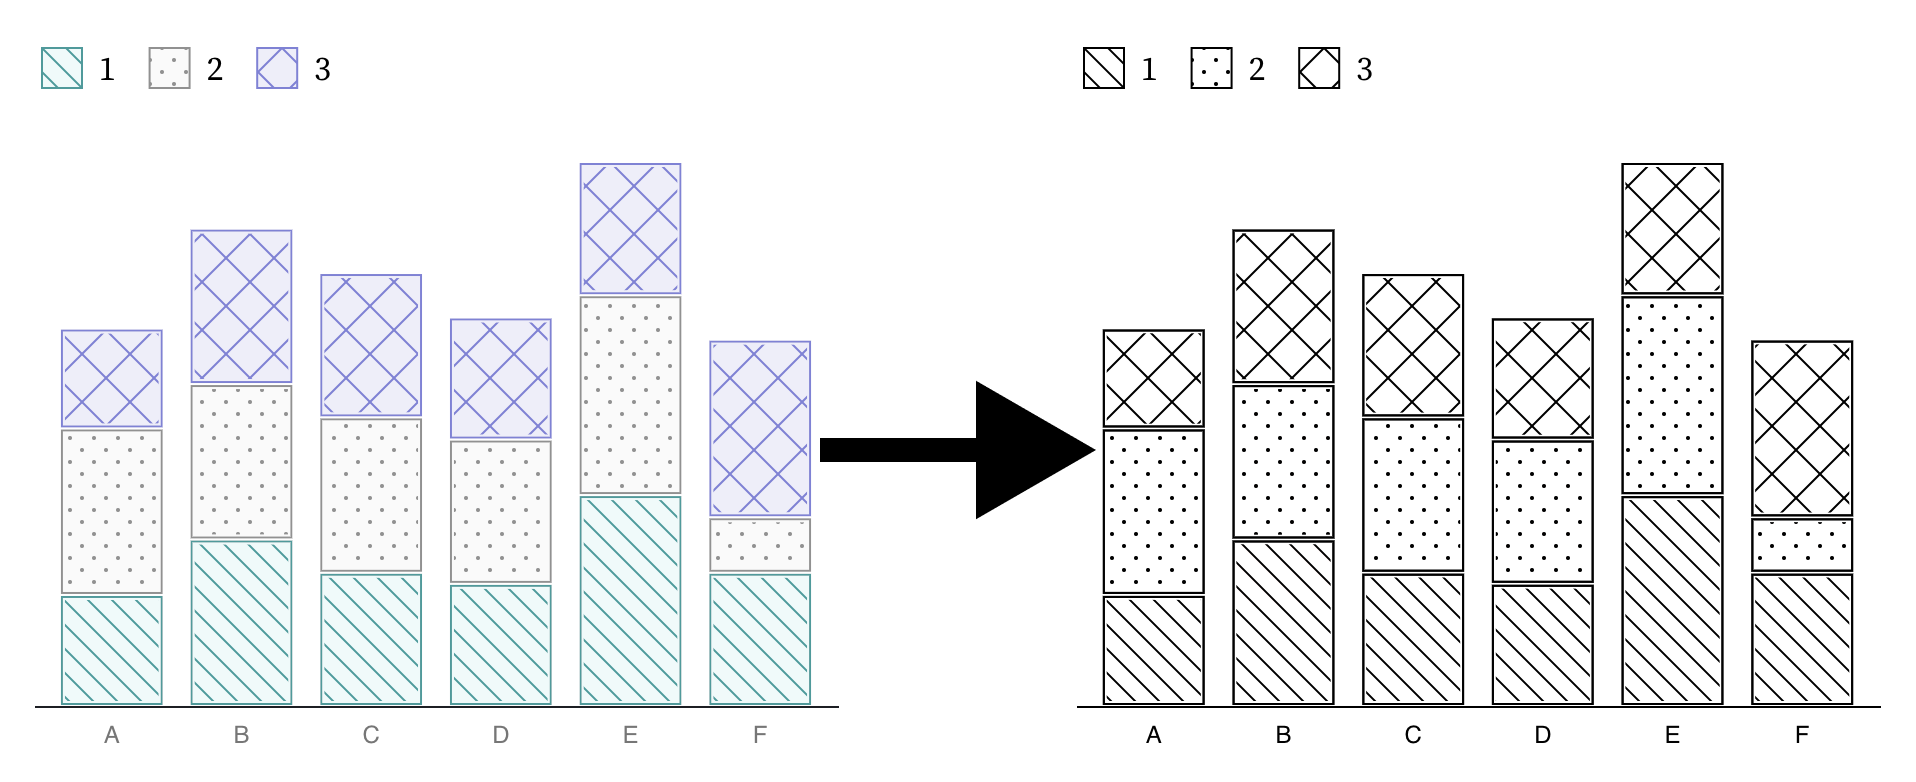
\includegraphics[width=0.75\linewidth]{figures/figure 9.png}
    \caption{A bar chart with categories (left) shown not conforming to Windows High Contrast White Mode. High contrast mode on Windows requires limiting color palettes, using only black or white for most elements (shown on the right).}
    \label{fig:9}
\end{figure}

Auditors should be especially critical of static designs, such as those that either use textures by default or not (\autoref{fig:9}), which are a high risk of compromising and assistive failure.

\section{Validating Chartability}

Next, Elavsky explains the preliminary user evaluation: I validated whether data practitioners felt more confident and equipped to make their own work accessible with Chartability. Additionally, I also wanted to interview expert accessibility practitioners (including those with disabilities) with the same questions, to see if Chartability had anything to offer in helping them understand and evaluate data experiences better. 

My secondary goal was to present a tool that can be helpful even in the wild on real projects (with all the weird design and engineering quirks that come with that). I wanted Chartability to be usable on things built with a tool like Tableau and fully bespoke, hand-coded visualizations, like those made with JavaScript and D3. To this secondary aim, I intentionally solicited participants who were working on a variety of different projects, each of their own design. 

\subsection{Pre-Validations and Flipped Roles: Participants Question \emph{Me}}

I performed several early, light validations of my work before soliciting and involving participants formally. My early pre-validations \#2-4 (below) all focused on practitioners asking me questions and giving feedback. 

My 4 pre-validations happened during the process of making Chartability, as well as introducing short iterations back into the making process: 

\begin{enumerate}
    \item \textbf{Beta Testing}: I performed several beta tests of Chartability during the process of making. I audited using versions that only had POUR principles, tried versions of Chartability that focused only on standards, and also tried out different iterations of the heuristics as I was forming them. This testing was important to perform early in the process because it helped me test the limits of various possible directions for this tool (standards-only, against standards, building off of standards, etc).
    \item \textbf{Early Advice}: After the first full pass of making Chartability was complete, I sent Chartability via email to 4 accessibility experts and 6 interested people with disabilities familiar with auditing in order to solicit open feedback. 
    \item \textbf{Professional Workshop}: I held a half-day professional workshop via zoom on auditing visualizations for accessibility and presented Chartability’s heuristics to this select audience of 50 participants. I demonstrated how to audit and then had a chance for feedback and questions.
    \item \textbf{Deep Feedback Session}: I presented Chartability to 14 experts on data visualization and accessibility, 5 of which are people with disabilities. I presented in two separate sessions through 2-hour video calls on zoom (roughly one hour was demonstration and one hour was discussion). 
\end{enumerate}

\subsection{Discovering ``Critical'' Heuristics}
\label{sec:critical heuristics}
These pre-validations helped me combine and divide some of the heuristics, adjust the language and phrasing, and label 10 specific tests as ``Critical,'' which can be seen in \autoref{tab:table}. These critical tests were ones that community members stressed as an important priority for one or more of the following reasons:
\begin{itemize}
    \item They are prohibitively expensive to fix late.
    \item The barriers they produce are too significant to ignore.
    \item They are among the most common type of accessibility failure.
    \item They affect many parts of a data experience.
\end{itemize}

All Critical heuristics are based on standards or research.

\subsection{Selecting Participants and Projects}
I was a practitioner and representing myself as a volunteer when I reached out to participants. At this stage in the project, I was still not affiliated with a research institution and was not interested in producing publishable knowledge. I intended to test Chartability in the wild and validate whether it achieved its aims. My priority was to collaborate with folks working on difficult problems or those who had a rare intersection of expertise between accessibility standards and interactive data experiences. To this end, I was highly permissive with potential collaborators in order to maximize the expertise of participants and breadth of environments for testing Chartability. 

However, part of being permissive with participants meant that I was willing to collaborate on projects that I cannot share in a research publication and many of my participants must remain anonymous (including interview results that contain sensitive information about intellectual property). Given that auditing is a field of work about identifying failures, there was both a high demand for participation in the evaluation of Chartability in tension with a low motivation to make these failures known in a public venue.

A summary of our selection process:
\begin{itemize}
    \item \textbf{Solicitation}: I reached out via email to 24 individuals in my network to participate in helping to evaluate Chartability. I mentioned that I wanted Chartability to be applied to a current project of theirs and was interested in performing some interviews about their experience before and after using Chartability. I mentioned up front that working with me would be uncompensated and potentially take multiple hours of their time (even multiple sessions) over zoom meetings.
    \item \textbf{Response}: 16 individuals were interested and shared their project details (2 would require an NDA to be signed). 
    \item \textbf{Selection}: I selected 8, based either on the expertise of the individuals, on the robustness of their project, and/or on the opportunity to get feedback about Chartability in team environments (which I didn't anticipate, but 3 of the 8 represented team efforts).
    \item \textbf{Resulting Group}: I worked with 19 total participants across 8 environment spaces.
    \item \textbf{Publishable Group}: Due to intellectual property concerns, I can publish interview results from 6 participants and discuss the details of 4 audit environments.
\end{itemize}

\textbf{Chris DeMartini}: a multi-year Tableau Zen Master and recognized expert visualization practitioner. His dashboard of a coin flipping probability game dataset that he produced with his daughter was the subject of his audit~\cite{DeMartiniCoin}. His audit only included criteria labelled Critical in Chartability (which involves only 10 tests instead of the full 45) and his dashboard failed 7 of them. A full audit was later conducted on Chris’s behalf. His full audit had a total 26 failures, 11 of which were considered non-applicable.\footnote{``Non-applicable:'' any test in the auditing process that does not contain content relevant to the test, such as ``Scrolling experiences cannot be adjusted or opted out of'' for a visualization that does not a scrolling input control\label{fnlabel}}

\textbf{Amber Thomas}: a data storyteller and technologist credited on 30 of The Pudding's visual essays. Amber has had a growing interest in accessibility challenges related to her line of work designing and developing state of the art, bespoke visual essays. Her article The Naked Truth was still in the early design and development stages when it was fully audited~\cite{AmakaNaked}. It failed 22 out of 45 tests, including 6 out of 10 criteria considered Critical. 6 tests were considered non-applicable.\footref{fnlabel}

\textbf{Sam} (self-selected pseudonym): a recognized design practitioner in the visualization community who lives with disability. They were collaborating on an interactive data project that would be specifically made to be used by international participants with a broad spectrum of disabilities. Their interactive infographic failed 21 out of 45 tests, 5 of which were considered Critical. 10 tests were considered non-applicable.\footref{fnlabel}

\textbf{Øystein Moseng}: Core Developer and Head of Accessibility of Highcharts. Øystein was interested in taking one of Highchart’s demo charts not specifically developed with accessibility features in mind~\cite{HighsoftHighcharts} and testing it against a full Chartability audit to see how it held up. The demo failed 13 out of 45 tests, 3 of which were Critical. 10 tests were considered non-applicable.\footref{fnlabel}

\textbf{Jennifer Zhang}: a senior accessibility program manager at Microsoft with expertise working on enterprise data products.

\textbf{Ryan Shugart}: a blind, screen reader user and disability subject matter expert at Microsoft who has a strong expertise in collaborative accessibility for interactive data systems. 

Both Shugart and Zhang were interested in applying Chartability internally and testing its effectiveness and potential with various projects. Their application and use of Chartability (including audits) are not available for publication, but their valuable interviews and evaluations are included with permission.

% *``Non-applicable:'' any test in the auditing process that that does not contain content relevant to the test, such as ``Scrolling experiences cannot be adjusted or opted out of'' for a visualization that does not a scrolling input control.

\section{Study Results}

I asked the 6 participants a series of qualitative and Likert-scale evaluation questions:

\begin{enumerate}
  \item Have you ever performed an audit of a data experience before?
  \item What stage of production is your project in? Analysis, design, prototyping, development, maintenance?
  \item How confident are you in your ability to perform an audit of a data experience for accessibility issues? (1-5, 1 being not confident at all, 5 being fully confident.)
  \item How difficult do you perceive auditing a data experience for accessibility issues is? (1-5, 1 being trivial, 5 being very difficult.)
  \item (After using Chartability) How confident are you in your ability to perform an audit of a data experience for accessibility issues? (1-5, 1 being not confident at all, 5 being fully confident.)
  \item (After using Chartability) How difficult do you perceive auditing a data experience for accessibility issues is? (1-5, 1 being trivial, 5 being very difficult.)
  \item (After using Chartability) Do you intend to continue using Chartability?
\end{enumerate}

Each of these questions had an open-ended question attached, ``Is there anything else you would like to add?'' Every participant provided additional input on questions 3 through 7. 

None of the 3 participants who only consider themselves expert data practitioners had performed an audit before. All 3 of them reported that they believed auditing to be easier and that they are more confident in their ability to evaluate the accessibility of data experiences after using Chartability. 

Of the 3 accessibility experts (all of whom have performed audits of data experiences before), their opinions on these measurements were unchanged after using Chartability. All 6 participants noted that they plan to use Chartability in their own work and would recommend it to their peers. 

Below we overview some of the key insights Elavsky received from the open ended responses.

\subsection{Real Access has more Considerations than Colorblindness}
Among the data practitioners, DeMartini wrote after his audit, ``I have read a lot about color blindness and could provide meaningful feedback to visualization developers on that topic, but I have come to realize that accessibility is so much more than this and I basically didn’t really know where to start when it came to the true scope of accessibility.'' He ended his qualitative feedback with, ``I think this could be a great tool for the masses and really look forward to the impact it can possibly have on the (inaccessible) data visualizations which are being created in huge numbers these days.''

\subsection{Audits are Slow, but Help me Focus}
Amber Thomas wrote, ``It still takes a while to do a complete audit, but it's not hard! For someone new to the space, all the possible options that can be used to make visualizations more accessible can be overwhelming. [Chartability] helped me to focus.'' She finished her feedback with, ``There aren't really guidelines (at least to my knowledge) that exist to help data visualization creators to ensure their work is accessible… [Chartability] helps to direct users to the most common accessibility problems with straightforward questions. It really helps to narrow the focus and prioritize efforts.'' 

\subsection{Chartability Helps me Remember and Stay Consistent}
Among the accessibility experts, Zhang wrote, ``While I am skilled, depending on the day I might not remember everything I need to look at. I am more confident in consistency between different auditing sessions. For experts it’s a good reminder framework.'' Moseng of Highcharts noted, ``[Chartability] did a very good job of highlighting concerns that are often ignored or forgotten when auditing and designing/developing.'' Shugart of Microsoft added along those lines, ``I feel [Chartability] arranges a good set of questions in a user’s mind and makes it easier for them to determine if a visualization is accessible.''

\subsection{Access is an Experience, not just Compliance}
Zhang offered insight into the design intention of Chartability, ``[it is] clearly going for above compliance and focusing on a good experience.'' Sam expressed their need to make an excellent accessibility experience, ``I am not just worried about compliance, but I want to make something really good. Nothing seems to help you go beyond? This is better than WCAG, I can already tell.''

\subsection{Everyone wants More Evaluation Resources and Tools}
For constructive feedback, all the data experts noted that they wanted more resources and materials related to learning the skills needed to conduct an audit. Shugart and Moseng both noted that they hope for more tooling and (in some cases) automated tests that can take the burden off the auditor and streamline the design and development process (much like Axe-core~\cite{Deque2021Axe}). They both also agreed that automation and tooling would help novice practitioners perform this work faster and with more confidence. 2 of the 3 mentioned wanting more examples of failures as well as accessible data experiences. Sam wrote that they felt Chartability was overwhelming at first, but after focusing on just the Critical items, the rest of the framework ``became easier.''

\subsection{Experts: ``Novices will Struggle.'' Novices: ``This was so helpful''}
The accessibility experts all unanimously agreed that Chartability is helpful to their own work, but they are unsure how accessibility novices would do. They all believe that more training and resources are needed to help people who are new, with one noting that Chartability could even be ``overwhelming'' to someone who has not been exposed to accessibility work before. All of the novices remarked that Chartability was ``so helpful,'' ``made this work so much clearer than before,'' and ``made a lot of hard problems not as hard.''

\subsection{What about Auditors with Disabilities?}
Shugart’s feedback was critical when discussing continuing to use Chartability, ``I still feel as a screen reader user, the audit itself would have some unique challenges because I’d be missing a lot and would have problems determining things such as color.'' He continued, ``Auditing anything accessibility-wise as a screen reader user poses challenges because you don’t always know what you’re missing. In many cases there are workarounds to this but datavis is one area where this is really hard to do now.'' 

\section{Extended Results}
Following calls to ensure accessibility work has practical benefits that exceed publications~\cite{Hurst2013Making}, in April, 2021 Elavsky made Chartability openly available on Github. As new research and practices emerge and more community members get involved, Chartability will become an evolving artifact of consensus similar to existing standards bodies~\cite{WAI2022WCAG3}.

Projects like Turkopticon benefited from the discussion about how a community actually used their tool~\cite{Irani2013Turkopticon}. In the same vein, we are happy to report some valuable findings from within this last year that we think demonstrate (in a pragmatic way) that Chartability has some merit: 
\begin{itemize}
    \item \textbf{It is living and growing}: Chartability has received enough community feedback that it is now on Version 2, with more tests and background resources provided.
    \item \textbf{People are talking about it}: Chartability has been featured in 14 workshops, talks, and podcasts and at least 2 university courses.
    \item \textbf{People are using it}: Chartability has contributed to projects at Microsoft, Highcharts, Project Jupyter, Fizz Studio, FiveThirtyEight, Vega-Lite, UCLA, the City of San Francisco, the Missouri School of Journalism, a fortune 50 company, two Fortune 500 companies, and community groups (like MiR).
    \item \textbf{It has breadth}: Chartability has evaluated static and interactive data experiences made with Microsoft's Excel and PowerBI, Tableau, JavaScript (D3, Vega-Lite, Highcharts, Visa Chart Components), Python (Altair, Bokeh, and matplotlib), R (ggplot2), as well as design sketches and low/medium-fidelity artifacts (Illustrator, Figma, Sketch).
\end{itemize}

When considering the analysis by Hurst and Kane about high abandonment rates in assistive technology,~\cite{Hurst2013Making} we wanted to make sure that we created an artifact (assistive technology or otherwise) that would at least survive its first year of use in the real world. 

The greater community feedback as well as new research before and after open-sourcing Chartability has also led to 5 new heuristics being added since our test users performed audits and gave evaluations. The current version of Chartability (v2) has a total of 50 heuristics. 

It is important to note that the work of Chartability did not begin and does not conclude with the publication of this manuscript. We want Chartability to become a living, community-driven effort that will adapt and grow as more resources, tools, and research become available.

\section{Discussion}
From our presentation of Chartability and a preliminary user evaluation with data visualization and accessibility practitioners, we learned that Chartability reduced the perception that working on accessibility is difficult and increased the confidence of those new to this work. Chartability shows promise as a useful framework for expert accessibility practitioners because it serves to produce consistency in contexts like the evaluation of dashboards, data science workflows, and other complex, data-driven interfaces. 

While our practitioners with novice accessibility experience were initially concerned about doing the audit correctly, most of their audit results were reasonably comparable with that of the authors (although their time to complete was much longer). 

We agree with experts that beyond Chartability, more resources are needed which provide examples of both inaccessible and accessible data visualizations as well as how to perform some of the more difficult parts of the auditing process (such as evaluating with a screen reader). We hope that keeping Chartability on GitHub will inspire future improvements to address this gap in examples, and will address future limitations, as we discover them. 

Chartability is a valuable tool for auditing. But we also hope that it can inspire researchers to:
\begin{enumerate}
    \item Examine which heuristics (in our supplemental materials) could use more research attention, particularly those labelled ``community practice.''
    \item Define constraints or requirements on novel projects, ensuring that new explorations still respects established standards, mitigating ethical risks.
    \item Explore the intersections of disability in ways yet unaddressed in standards, such as the strong overlaps between understandability and operability (like keyboard navigation patterns across a data structure) or conflicts in understandability and flexibility (how some users need redundant encodings on charts while others find this overwhelming).
    \item Consider access barriers in data experiences beyond those related to visual perception.
    \item Engage the relationship between labor and access in computing, such as developing more measurements that demonstrate the imbalance of time and effort expected of users with disabilities (even in systems considered to provide ``equal'' access) and ways to evaluate who is contributing to accessibility efforts in a project (core team members, contractors, or volunteers).
\end{enumerate}

We also want to caution researchers who are considering developing heuristics or auditing tools for use in practitioner environments to consider the tradeoffs between evaluation in rich, authentic professional settings and concerns such as intellectual property and corporate branding. We were able to apply our work in rich and collaborative practitioner settings because we were permissive with our potential participants. However, much of this work exists behind closed doors, similar to the downsides of industry research settings. More work may need to be done in order to encourage rich, cross-industry research projects, such as helping to anonymize the content of intellectual property and not just participants, while retaining data and findings. 

\section{Conclusion}

The demand for accessible data experiences is long overdue. The Web Accessibility Initiative’s (WAI) Web Content Accessibility Guidelines (WCAG) are over 22 years old and yet little work has been done to synthesize this large body of existing accessibility standards with research and inclusive design principles relevant to the fields of data communication, data science, data analysis, and visualization. Chartability begins to address unique accessibility best practice gaps in these domains with specific heuristics. This synthesis is meant to empower researchers, analysts, designers, developers, editors, and accessibility specialists with a framework to audit the accessibility of data experiences, interfaces, and systems to produce more inclusive environments for users with disabilities. The goal of Chartability is to make this work easier in order to encourage practitioners to regard current practices and resources, some of which have existed for decades. 

In addition, Chartability opens the door to more work that remains to be explored in this space. Additional research is needed into many of the topic areas within Chartability’s heuristic principles (POUR+CAF) as well as resources, examples, and tools provided for practitioners to perform this work more confidently and efficiently. 

The changing landscape of visualization techniques and alternative interfaces (such as sonification and dynamic tactile graphics) may increase the demands for accessibility considerations in this space. The growing technological divide will become an even greater human rights issue as time moves on and we believe that tools like Chartability are necessary for the community of data practitioners to ensure they are including people with disabilities.

\part{Navigation: Making Data Structures Traversable}

\chapter{\textit{Data Navigator}: Low-level Tooling for Creating Navigable Data Structures}

\noindent\rule{16cm}{0.4pt}
\begin{quote}
This chapter was adapted from my published paper:
\begin{adjustwidth}{1cm}{}
% \-\hspace{2cm}
F. Elavsky, L. Nadolskis, and D. Moritz, ‘Data Navigator: An Accessibility-Centered Data Navigation Toolkit’, \textit{IEEE Transactions on Visualization and Computer Graphics}, pp. 1–11, 2023.
\end{adjustwidth}
\end{quote}
\noindent\rule{16cm}{0.4pt}

\section{Abstract}

Making data visualizations accessible for people with disabilities remains a significant challenge in current practitioner efforts. Existing visualizations often lack an underlying navigable structure, fail to engage necessary input modalities, and rely heavily on visual-only rendering practices. These limitations exclude people with disabilities, especially users of assistive technologies. To address these challenges, we present Data Navigator: a system built on a dynamic graph structure, enabling developers to construct navigable lists, trees, graphs, and flows as well as spatial, diagrammatic, and geographic relations. Data Navigator supports a wide range of input modalities: screen reader, keyboard, speech, gesture detection, and even fabricated assistive devices. We present 3 case examples with Data Navigator, demonstrating we can provide accessible navigation structures on top of raster images, integrate with existing toolkits at scale, and rapidly develop novel prototypes. Data Navigator is a step towards making accessible data visualizations easier to design and implement.

\section{Overview}
\begin{figure}[h]% specify a combination of t, b, p, or h for top, bottom, on its own page, or here
  \centering % avoid the use of \begin{center}...\end{center} and use \centering instead (more compact)
  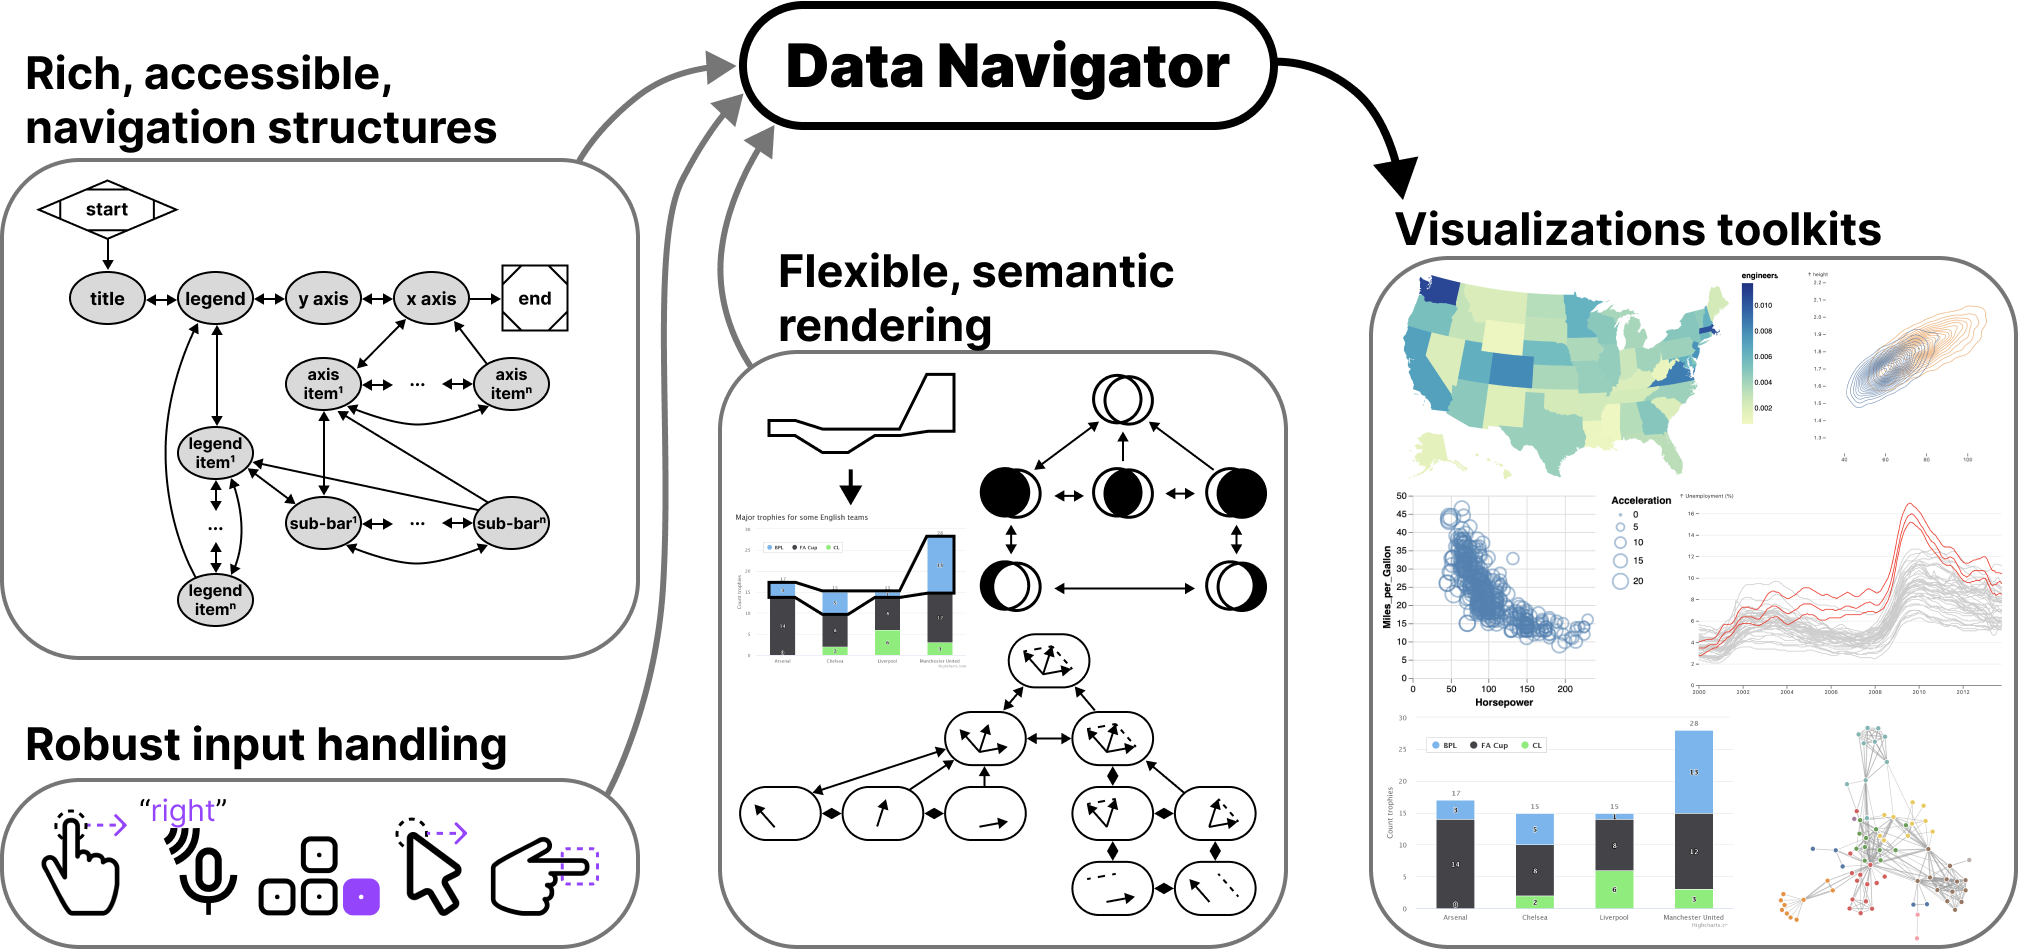
\includegraphics[width=\linewidth, alt={A schematic of a device with a rail and two handles. This device manipulates a chart and a separate chart is rendered as a tactile graph on a refreshable braille display.}]{data_navigator.png}
  \caption{%
  	Data Navigator provides data visualization libraries and toolkits with accessible data navigation structures, robust input handling, and flexible semantic rendering capabilities.%
  }
  \label{fig:data_navigator}
\end{figure}
While there is a growing interest in making data visualizations more accessible for people with disabilities, current toolkit and practitioner efforts have not risen to the challenge at scale. Major data visualization tools and ecosystems predominantly produce inaccessible artifacts for many users with disabilities. We believe this is largely a gap caused by a lack of underlying structure in most visualizations, failure to engage the input modalities used by people with disabilities, and over-reliance on visual-only rendering practices.

Users who are blind or low vision commonly use screen readers and users with motor and dexterity disabilities often do not use ``pointer'' (precise mouse and touch) based input technology when interacting with digital interfaces. Many users with motor and dexterity disabilities use discrete navigation controls, either sequentially using keyboard-like input, or directly using voice or text commands.

Most interactive visualizations simply focus on pointer-based input: they can be clicked or tapped, hovered, and selected in order to perform analytical tasks. This excludes non-pointer input technologies. These devices require consideration for the navigation structure and underlying semantics of a visual interface.

However, building navigable spatial and relational interfaces is a difficult task with current resources.

Raster images, arguably the most common format for creating and disseminating data visualizations, currently cannot be made into navigable structures. These are only described using alt text, which limits their usefulness to screen reader users.

Unfortunately, more accessible rendering formats like SVG with ARIA (accessible rich internet applications) properties are more resource intensive than raster approaches, like WebGL-powered HTML canvas or pre-rendered PNG files. SVG puts a burden on low-bandwidth users and a ceiling on how many data points can be rendered in memory.

In addition, ARIA itself has 2 major limitations. First, when added to interface elements, ARIA only provides \textit{screen reader} access, which means that developers must build a solution from scratch for other navigation input modalities. Second, ARIA's linear navigation structure can be time-consuming for screen reader users if a visualization has many elements. This may impede how essential insights and relationships are understood~\cite{Sorge2016Polyfilling,Godfrey2018Accessible,Zong2022Rich,Thompson2023Chart,Jung2022Communicating,Sharif2021}.

Some emerging approaches have sought to address this serial limitation of data navigation and provide richer experiences for screen reader users~\cite{Sorge2016Polyfilling,Godfrey2018Accessible,Zong2022Rich,Thompson2023Chart}. However, these approaches rely on a tree-based navigation structure which is often not an appropriate choice for visualizations of relational, spatial, diagrammatic, or geographic data. Many visualization structures are currently unaddressed.

Zong \ea stress that in order to realize richer, more accessible data visualizations, the responsibility must be shared by ``toolkit makers,'' the practitioners who design, build, and maintain visualization authoring technologies~\cite{Zong2022Rich}. Our contribution is towards that aim, to make more accessible data experiences easier to design and implement within existing visualization work.

We present Data Navigator. Data Navigator is a toolkit built on a graph data structure, within which a broad array of common data structures can be expressed (including list, tree, graph, relational, spatial, diagrammatic, and geographic structures). Data Navigator also exposes an interface that supports interactions via screen reader, keyboard, gesture-based touch, motion gesture, voice, as well as fabricated and DIY input modalities. Data Navigator provides expressive structure and semantic rendering capabilities as well as the ability for developers to use their own, preferred method of rendering.

Data Navigator builds upon human-studies motivated work on accessible navigation~\cite{Zong2022Rich,Thompson2023Chart} towards a more generalizable resource for visualization practitioners. We contribute a high-level system design for our node-edge graph-based solution as well as an implementation of this system on the web, using JavaScript, HTML, and CSS. Through our case examples we also demonstrate that our generalized approach is suitable for replication of existing best practices from other systems, integration into existing visualization toolkit ecosystems, and development of novel prototypes for accessible navigation. We illustrate how Data Navigator's use of generic edges, dynamic navigation rules, and loose coupling between navigation and visual encodings provides practitioners robust, expressive, control over their system designs.

\section{Related Work}
Our contribution is an attempt to bridge the gap between research and practice more effectively across broad ecosystems in order to enable deeper and more expressive accessible data navigation interfaces. Below we outline the prior research and standards that inform our project, a breakdown of existing visualization toolkit approaches to data navigation, and then accessible input device considerations.

\subsection{Accessibility research and standards in visualization}
Research and standards are both somewhat limited by a strong bias towards visual disabilities. In \textit{Chartability}, 36 of the 50 criteria related to accessible visualization considerations involve visual disabilities~\cite{Elavsky2022Chartability, Fan2023Accessibility}. Marriott \ea also found that visual disability considerations are the primary focus of data visualization literature~\cite{Marriott}, leaving the barriers that many other demographics face unstudied.

However, despite the heavy focus on visual disabilities, the work that does exist in the visualization community is deeply valuable and serves as an important starting point for our technical contribution.

\subsubsection{Accessible navigation design considerations}

Zong \ea's research, which was conducted as in-depth co-design work and validated in usability studies involving blind participants, presented a design space for accessible, rich screen reader navigation of data visualizations. They organized their design space into \textit{structure, navigation,} and \textit{description} considerations and demonstrated example \textit{structural}, \textit{spatial}, and \textit{direct} tree-based approaches~\cite{Zong2022Rich}.

\textit{Chart Reader} also engaged these design space considerations in their co-design work on accessible data navigation structures~\cite{Thompson2023Chart}. We consider these design dimensions as the best starting point for our work, bridging the gap between research and toolkits.

There are additional research projects that have focused on accessible data navigation and interaction ~\cite{Sharif2022VoxLens,Sorge2016Polyfilling,Godfrey2018Accessible,Sharif2018evoGraphs}. These contributions explore a range of different interaction structures, including lists, trees, and tables of information as well as direct access methods such as voice interface commands and simple, pre-determined questions.

\subsubsection{Accessible visualization: understanding users}

A wide array of emerging research projects investigate screen reader users needs, barriers, and preferences, and offer guidelines, models, and considerations for creating accessible data visualizations~\cite{Sharif2021,Lundgard2022Accessible,Chundury2022Towards,Fan2023Accessibility}. Jung \ea offer guidance to consider the order of information in textual descriptions and during navigation~\cite{Jung2022Communicating}. Kim \ea collected screen reader users' questions when interacting with data visualizations, which could open the door for more natural language data interaction~\cite{Kim2023Exploring}.

\subsubsection{Accessibility standards and guidelines}
In the space of research, there has been a growing interest in developing guidelines for practitioners~\cite{Elavsky2022Chartability, Durant2022Ten} and even applying guidelines as a method of validation alongside human studies evaluations and co-design~\cite{Lundgard2019Sociotechnical,Zong2022Rich,Lundgard2022Accessible,Fan2023Accessibility}. Unfortunately, most accessibility standards and guidelines do not explicitly engage how to structure data navigation. 

Despite this, existing accessibility standards bodies like the Web Content Accessibility Guidelines do stress the importance of accurate, functional semantics in order for screen reader users to know how to interact with elements~\cite{WAI2021Semantics}. For interactive visualizations this means that button-like or link-like behavior should expressly be made using elements that are semantically buttons and links. Our system should be capable of expressing meaningful semantics to users of assistive technologies.

\subsection{Visualization toolkits and technical work}
Unfortunately while many data visualization toolkits offer some degree of accessible navigation and interaction capabilities to developers, very few toolkits currently out there offer control over the important aspects of accessible data navigation design. Replicating existing research and strategies, remediating toolkit ecosystems, and building novel prototypes are all difficult or impossible to do due to the current lack of toolkit capabilities.

Existing data visualization toolkits have 3 major limitations that we wanted to address in the design of Data Navigator:
\begin{enumerate}
  \itemsep-0.4em
  \item \textbf{Built on visual materials}: toolkits produce either raster or SVG-based visualizations, neither of which are focused towards designing navigable, semantic structures. As a consequence, many visualizations are simply entirely inaccessible.
  \item \textbf{Lacking relational expressiveness}: When data navigation \textit{is} provided, the navigation is based on either a tree or list structure (see~\Cref{existing}). The consequence of this limitation is that many other non-list and non-tree data relationships become difficult or impossible to represent without overly tedious navigation or inefficient architecture.
  \item \textbf{Designed only for screen reader interaction}: When \textit{accessible} data navigation is provided, it is generally only made possible through SVG with ARIA (Accessible Rich Internet Application) attributes. ARIA is primarily only leveraged by screen readers~\cite{WAI2017ARIA}. If a data element can be clicked and performs some form of function, only direct pointer (mouse and touch) and screen reader users are included. The consequence of this is that a wide array of other input devices, many used as assistive technologies by people with motor and dexterity disabilities, are excluded.
\end{enumerate}

\begin{figure}[h]
  \centering
  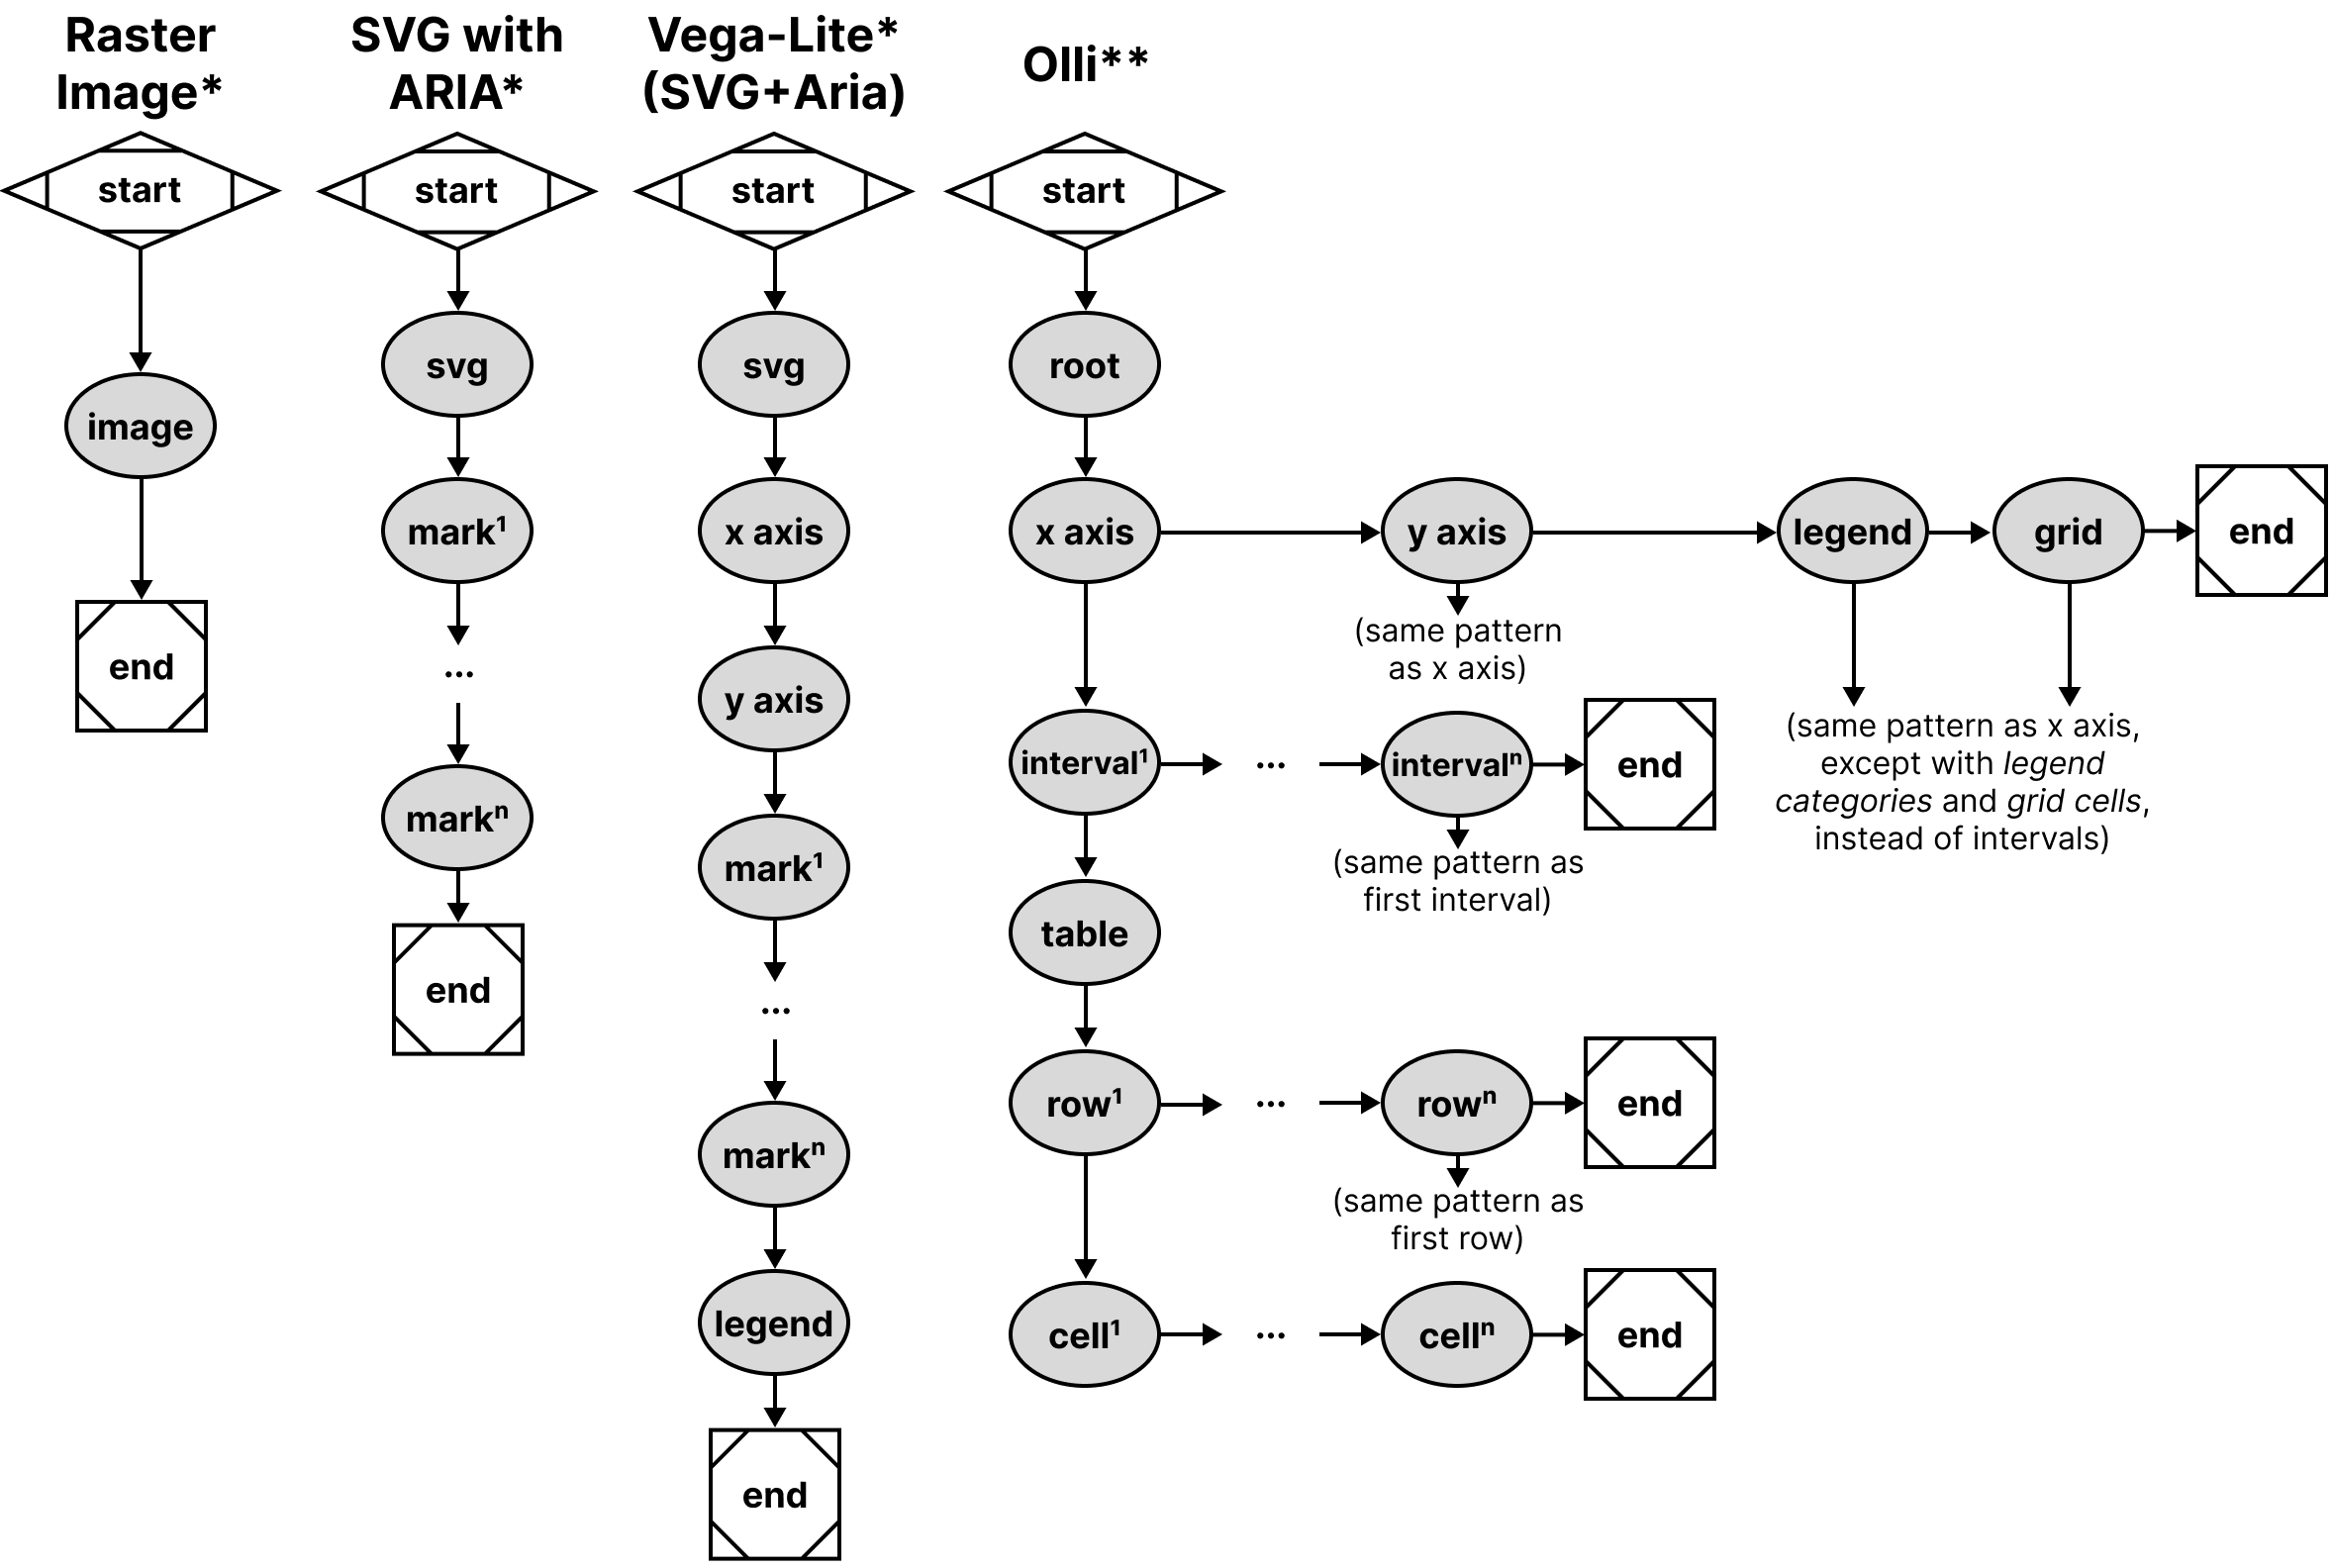
\includegraphics[width=12cm,height=12cm,keepaspectratio]{figures/state-of-the-art.png}
  \caption{Existing accessibility trees and lists, shown using node-edge graph conventions. (*) Denotes only \textit{screen reader} access. (**) Denotes \textit{screen reader}, \textit{keyboard-only}, and \textit{pointer} access as well.}
  % \Description{A mouse pointer is shown shaking over many data points that are very small while a touch hit area is shown over the same visualization, overlapping with many points at once.}
  \label{existing}
\end{figure}

\subsubsection{Rich, tree-based approaches}
De-coupling rendered, visual structures from meaningful and effective navigation experiences can provide richer experiences for screen reader users~\cite{Zong2022Rich}. Prior research and industry work, with the exception of the \textit{Visa Chart Components} library~\cite{VisaVisa}, has relied heavily on a 1 to 1 relationship between structure (the encoded marks) and navigation. This emerging work is significant, because it paves the way for considering the design dimensions of accessible data interaction and navigation without dependence on a visually encoded space.

\textit{Olli's} approach has been to build ready-to-go adaptors that automatically build multiple tree structures for a few ecosystems (\textit{Vega}, \textit{Vega-Lite}, and \textit{Observable Plot}) and is entirely uncoupled from a data visualization's graphics. Their approach renders navigable tree structures \textit{underneath} a visualization.

Other than \textit{Olli}, \textit{Highcharts}~\cite{HighsoftHighcharts}, \textit{Visa Chart Components}, and \textit{Progressive Accessibility Solutions'} visualization toolkits~\cite{Sorge2016Polyfilling,Godfrey2018Accessible} also primarily provide tree and list navigation structures across all of their chart types. These toolkits render their structures \textit{upon} the visualization's graphic space. These tools also provide some degree of support for other assistive technologies and input modalities, although are limited exclusively to SVG rendering. 

Unfortunately, these toolkits lack capabilities for dealing with graph, relational, spatial, diagrammatic, and geographic data structures.

\subsubsection{Serial, list-based approaches}
Toolkits like \textit{Vega-Lite}~\cite{Satyanarayan2017VegaLite} and \textit{Observable Plot} only provide basic screen reader support through ARIA attributes when visualizations are rendered using SVG. These libraries do not currently provide additional access to other assistive technologies and input modalities.

Microsoft's \textit{PowerBI} largely uses a serial structure, although it has tree-like elements as well. \textit{PowerBI} generally provides the same access to keyboard users as it does to screen readers, although not completely.

\subsubsection{No navigation provided}
Other visualization tools, like \textit{ggplot2} or \textit{Datawrapper}, \textit{Tableau}, as well as both \textit{Vega-Lite} and \textit{Highcharts} (when rendering to canvas), produce raster images and have no navigable structure available. Raster, or pixel-based graphics have been an accessibility burden since the early days of graphical user interface development~\cite{Boyd1990Graphical}. Practitioners who use these toolkits can only provide alternative text.

% \subsubsection{Automatic description generation}
% A considerable amount of data visualization and accessibility literature focuses on technical contributions that look to automate alt text descriptions or captions for data visualizations ~\cite{Choi2019Visualizing,Balaji2018Chart,Chen2019Neural,Chen2020Figure,Lai2020Automatic,Obeid2020Chart,Qian2021Generating,Sharif2018evoGraphs}. 

% Most recent work by Kim \ea built a prototype that automatically converts a chart specification of a treemap into a description and tested it with blind users~\cite{Kim2023Explain}. While technical contributions that attempt to automate description generation through deterministic or model-driven approaches are closely related to our project and on-going, our interest is primarily in a different direction than hands-off automation: providing developers with a robust ability to express the design dimensions of a data navigation scheme.

\subsection{Considering assistive technologies and input devices}
Modern data visualizations may contain functional capabilities such as the ability to hover, click, select, drag, or perform some analytical tasks over the elements of the visualization space~\cite{Satyanarayan2017VegaLite}. Virtually all of these analytical capabilities are designed for use with a mouse.

Input device consideration can roughly be organized as either \textit{pointer-based} (such as a mouse or direct touch) or \textit{non-pointer based} (which may employ speech recognition or sequential, discrete navigation such as with a keyboard). Assistive pointer-based devices, such as a head-mounted touch stylus, can typically perform any actions that a mouse can and are therefore served by current interactive visualizations. However, assistive non-pointer devices, such as a tongue, foot, or breath-operated switch, are not.

By only providing pointer-based interactivity, modern interactive visualizations exclude users who leverage non-pointer based input, who are most commonly people with motor and dexterity disabilities. And unfortunately, there is a complete lack of engagement with these populations in the data visualization research community~\cite{Marriott}.

By comparison, the broader accessibility and HCI research communities have rich engagement with interaction and assistive technologies for users with motor and dexterity disabilities. Most research either focuses broadly on physical peripheral devices or sensors~\cite{Siean2021}, wearables~\cite{Sarsenbayeva2022}, or DIY making and fabrication~\cite{Hurst2013Making}.

The DIY making space involves a broad spectrum of complex input devices and materials, such as fabricating with wood and sensors for children with disabilities~\cite{Lin2014}, 3D printed materials for rehabilitation professionals~\cite{Giraud2016}, and even using produce-based input (such as bananas and cucumbers) for aging populations~\cite{Rogers2014}.

Broadly, both research and practical developments related to accessible, non-pointer input are much further ahead than data visualization research and practice. Our goal for Data Navigator is to provide a technical resource towards engaging this under-addressed space.

\section{Data Navigator: System Design}
% \begin{figure}[h]
%   \centering
%   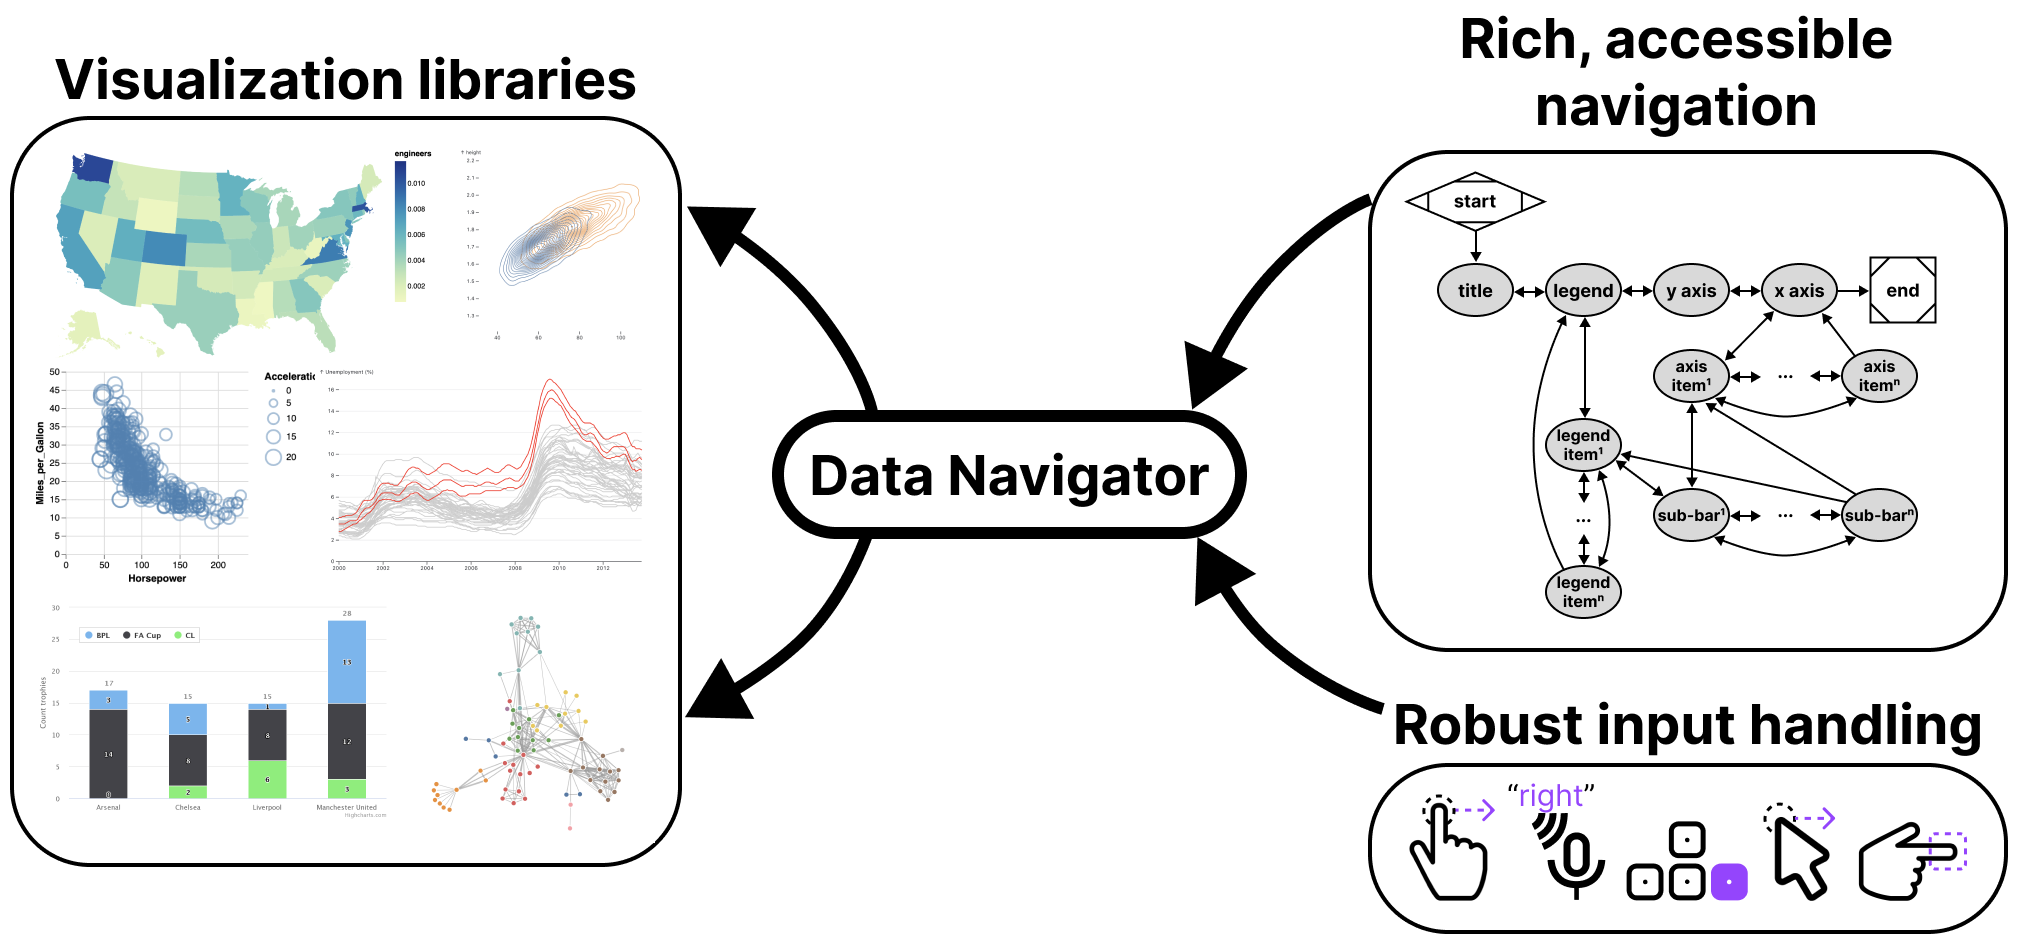
\includegraphics[width=\linewidth]{figures/system-design.png}
%   \caption{Data Navigator provides data visualization libraries and toolkits with accessible data navigation structures and robust input handling.}
%   \label{pointer}
% \end{figure}

We categorized our system design goals into design considerations for \textit{Structure}, \textit{Input}, and \textit{Rendering}:
\begin{enumerate}
  \itemsep-0.4em
  \item \textbf{Generic structure and navigation specification}: Human studies work has validated that lists, tables, trees, and even pseudo-treelike and direct structure types are all valuable to users in different contexts and with different considerations. Our system must be able to work with all of these as well as less frequently-used structures (spatial, relational, geographic, graph, and diagrammatic).
  \item \textbf{Robust input handling}: Blind and low vision users may use combinations of different assistive technologies, such as magnifiers, voice interfaces, and screen readers. Users with motor impairments may rely on voice, gesture, eye-tracking, keyboard-interface peripherals (like sip-and-puffs or switches), or fabricated devices. Both the developer and user should therefore be able to leverage and customize a broad range of input types, including the above as well as fabricated, adaptive, and future input modalities.
  \item \textbf{Flexible rendering and semantics}: Visuals may or may not be necessary to render to demonstrate Data Navigator's structure. In addition, much of the latest research has shown that different screen reader users may prefer different orders of information and at different levels of verbosity. In addition, the context of tasks the user is performing as well as the nature of the data itself may influence the design of semantic descriptions and visual indications for elements. Data Navigator must provide a high degree of flexibility and control.
\end{enumerate}

To help bridge the gaps between research and standards knowledge about best practices and building an effective toolkit for practitioners, we intend for Data Navigator to provide both \textit{exploratory support} and \textit{vocabulary correspondence}~\cite{Maayan2020Domain}.

In particular, our ideal users are developers who specify data visualizations using code. To that aim, we intend to provide \textit{exploratory support} through generic, dynamic, and flexible system design decisions. Our system is expressive and customizable, which encourages exploration of different options.

And we also want the API to include properties that have conceptual and \textit{vocabulary correspondence} to our design considerations. Each design consideration (\textit{Structure}, \textit{Input}, and \textit{Rendering}) are separately composable, modular subsystems of Data Navigator that can be used independently or in tandem with one another.

% The first major contribution in the design of Data Navigator is to use node-edge data as the substrate for our navigation system. In a generic Backus-Naur Form~\cite{Backus1963Revised}, the high level details of our system grammar are as follows:

% \begin{lstlisting}[
%     basicstyle=\small
% ]
%  <dn> ::= <structure> <navigation> <rendering>
%  <structure> ::= <nodes> <edges>
%  <navigation> ::= <nav-rule>+
%  <nodes> ::= <node>+
%  <edges> ::= <edge>+
%  <rendering> ::= <location> <id> <dimensions> [<on-demand>]
%  <nav-rule> ::= <name> <edge-types> <direction> [<inputs>]
%  <node> ::= <id> <datum> [<spatial>] <edge-ids> <semantics>
%  <edge> ::= <id> <source> <target> <edge-type>
%  <spatial> ::= <coords> <shape>
%  <coords> ::= <x> <y>
%  <shape> ::= <dimensions> | <path>
%  <dimensions> ::= <width> <height>
%  <source> ::= source() | <id>
%  <target> ::= target() | <id>
%  <semantics> ::= <element-type> <role> <description>
% \end{lstlisting}

In this paper we present an implementation of our system using JavaScript, HTML, and CSS on the web. The demonstration of our system is best suited to the web due to the nature of existing, accessible building blocks (HTML), which resolve many of the semantic complexities and logic involved in enabling screen readers to programmatically navigate and announce meaningful information to users. In addition, many existing visualization toolkits target the web as an output platform and we believe that this is the best starting point for adoption and use of Data Navigator. However, this system design could be implemented as a toolkit in other environments with proper consideration for input device handling and screen reader semantics.

\subsection{Structure}
% \begin{lstlisting}[
%     basicstyle=\small
% ]
%  <dn> ::= <structure> <input> <rendering>
% \end{lstlisting}
\subsubsection{Beyond trees: towards an accessibility \textit{graph}}

The first major contribution in the design of Data Navigator is to use node-edge data as the substrate for our navigation system.

The most important argument in favor of using a graph-based approach is that a graph can construct virtually any other data structure type (see \Cref{existing}), including list, table, tree, spatial, geographic, and diagrammatic structures. Graphs are generic, which enables them to represent structures both in current and future interface practices~\cite{Gansner2000Open}.

\begin{figure}[h]
  \centering
  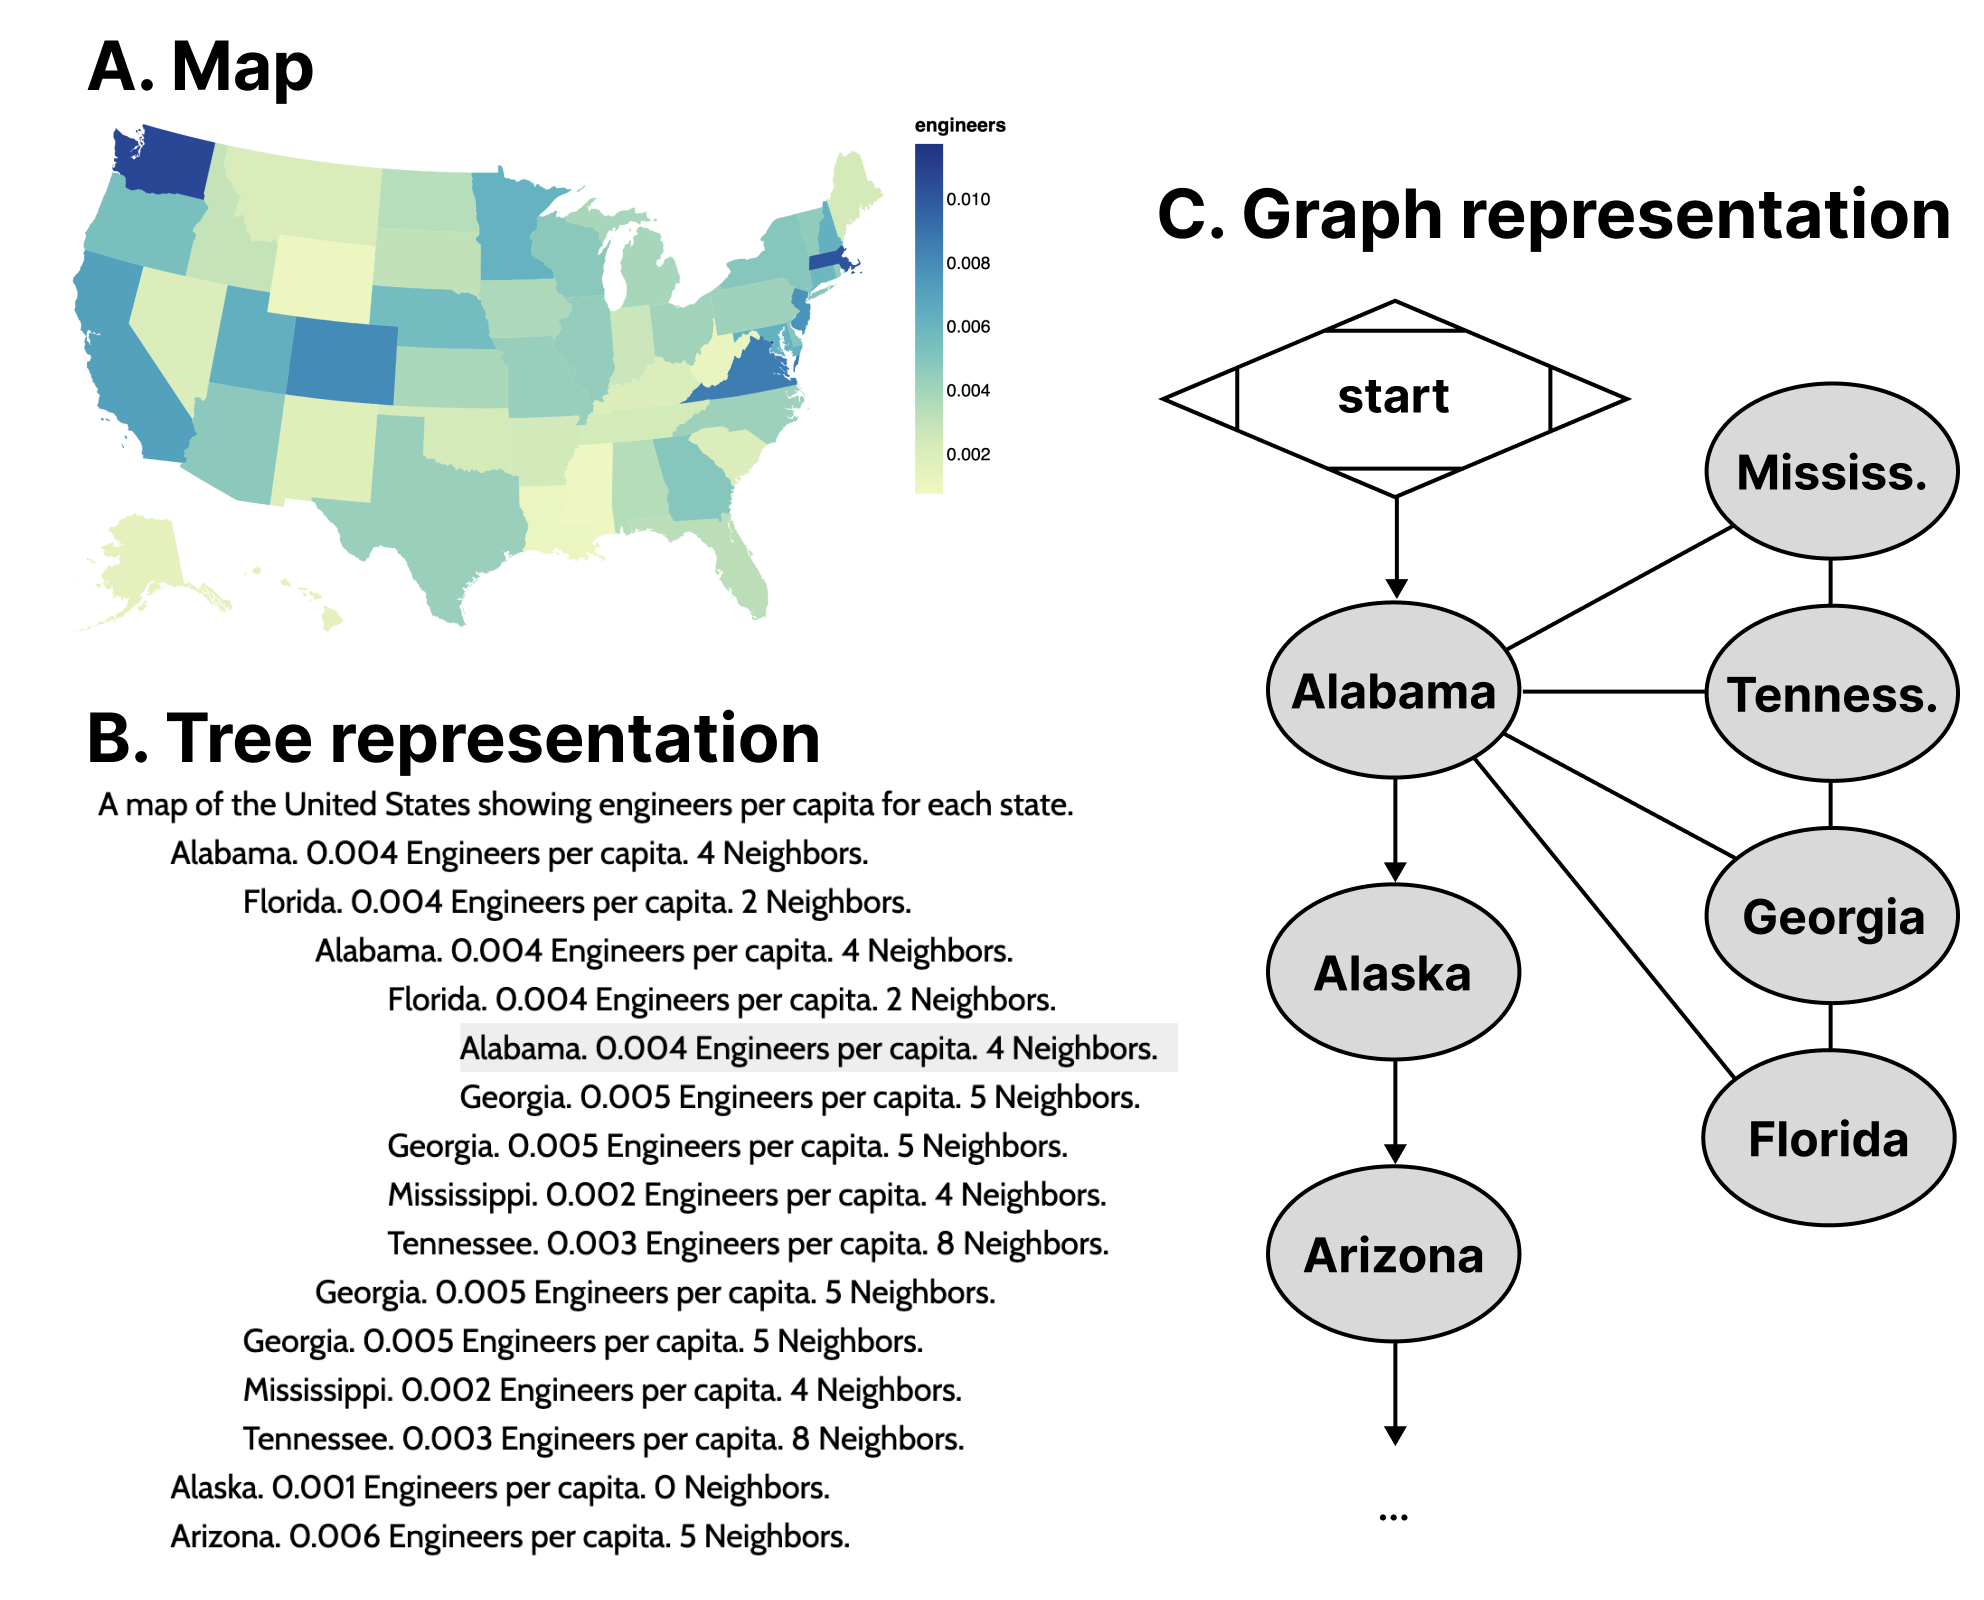
\includegraphics[width=0.65\linewidth]{figures/geoviz.png}
  \caption{\textbf{A.} Map of engineers per capita of US states. \textbf{B.} Tree representation of the map data where states are listed alphabetically and also include links to neighboring states. The structure repeats itself if users navigate in a loop. \textbf{C.} Graph representation with the same navigation potential without redundant rendering.}
  % \Description{A mouse pointer is shown shaking over many data points that are very small while a touch hit area is shown over the same visualization, overlapping with many points at once.}
  \label{map}
\end{figure}

To demonstrate our point, the most recent emerging work with advancements in accessible data navigation used node-edge diagrams to demonstrate their tree-like structures~\cite{Zong2022Rich, Thompson2023Chart} similar to \Cref{existing}, \Cref{static}, and \Cref{vega-lite}. This is because trees are a form of node-edge graph, but with a root, siblings, parents, and children as sub-types of nodes that generally have rules for how they relate to one another. 

Node-edge graph structures prioritize direct relationships. Examples of common direct relationships in visualization are boundaries on maps (see \Cref{map}), flows and cycles, data with multiple high level tree structures pointing to the same child datasets (such as \textit{Olli} in \Cref{existing}), or even just in diagrammatic, graph-based visualizations.

A graph structure allows for direct access between information elements that are not just part of the input data or 1:1 rendered elements, but may also have perceptual or human-attributed meaning. Examples of this might include semantic or task-based relationships, such as navigating to annotations or callouts, between visual-analytic features like trends, comparisons, or outliers. Spatial layouts such as intersections of sets or parallel vectors (see \Cref{section:codesign}), or even relationships to information outside of a visualization and back into it (like in \Cref{semantics}) are enabled by a graph structure.

\subsubsection{Graph structures are more computationally efficient}

Data visualizations often portray information that becomes difficult to handle when using trees and lists. The distance users must travel between relational elements is significant in lists while redundancy when navigating relational elements in trees can be problematic.

As an example of this, often a data table or list of locations are used in conjunction to a map, such as listing all 50 states alphabetically along with relevant information. The list itself is expensive to navigate and may not provide any relationship information about which states border others, let alone ways to easily and directly access those states.

Part of the visual design justification of using a map instead of a table is for sighted individuals to understand how geospatial information may interact with a given variable. The spatial relationships matter. But when supplementing the list of states with sub-lists for each state's bordering states (see \Cref{map}), it produces redundancy in the rendered result. The rendered data contains circular connections between nodes but must render every reference, producing a computational resource creep and cluttered user experience that can be difficult to exit.

\subsubsection{Specific edge instances and generic edges}
\begin{figure}[h]
  \centering
  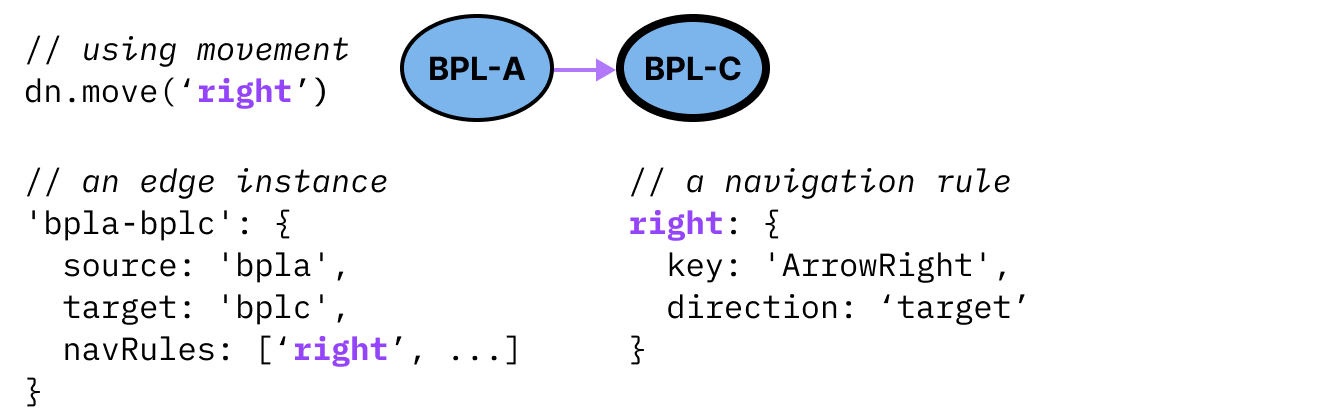
\includegraphics[width=0.75\linewidth]{figures/simple_movement.png}
  \caption{An example of how a single edge instance references a navigation rule and can even have multiple navigation rules. A navigation rule can be referenced by multiple edges.}
  % \Description{A mouse pointer is shown shaking over many data points that are very small while a touch hit area is shown over the same visualization, overlapping with many points at once.}
  \label{simple_movement}
\end{figure}

In Data Navigator, nodes are \textit{objects} that always contain a set of edges, where each edge contains a minimum of 4 pieces of information: a unique identifier, a source, a target, and navigation rules. These properties are only accessed when a navigation event occurs on a node with an edge that contains a reference to a rule for that navigation event. Navigation rules may be unique to an edge instance or shared among other edge instances.

The source and target properties of edges are either ids that reference node instances (see \Cref{simple_movement}) or \textit{functions} (see \Cref{dynamic_movement}). Because some edges in a graph may be directed or not, non-directed graphs can use source and target properties to arbitrarily refer to either node attached to an edge.

Generic functions for source or target properties can link nodes to other nodes based on changing content, structure, or behavior that may be difficult or impossible to determine before a user navigates the structure.

Function calling also allows some edges to be \textit{purely} generic. An example of a reasonable use case of a purely generic edge is in \Cref{dynamic_movement}, where the source is a function which returns the present node and the target is whichever node the user was on previously. This single edge may then be part of every node's set of edges, enabling users to have a simple \textit{undo} navigation control without creating an \textit{undo} edge unique to every source node.

Using this pattern, it is possible to have fully navigable structures using only generic edges.

\begin{figure}[h]
  \centering
  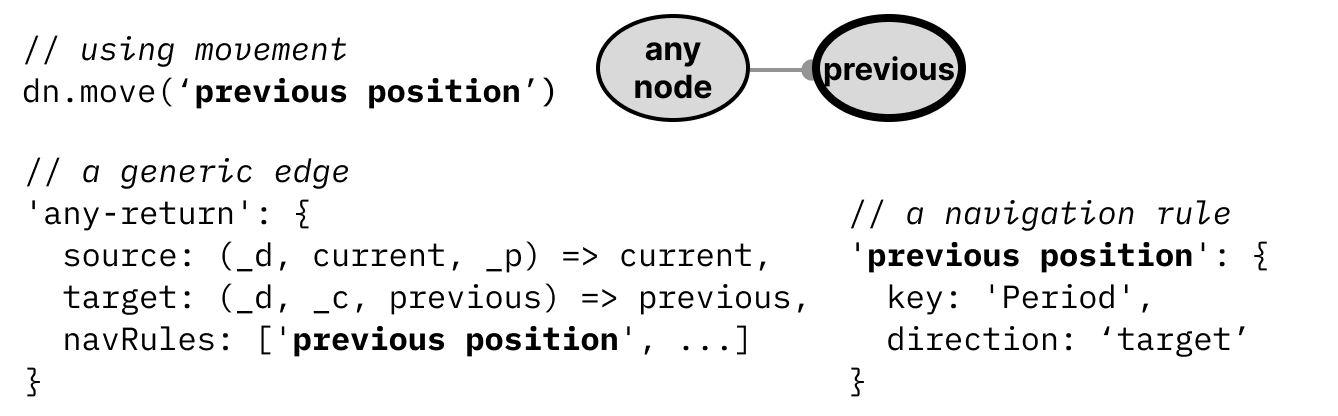
\includegraphics[width=0.75\linewidth]{figures/dynamic_movement.png}
  \caption{A generic edge, such as ``any-return'' can be applied to any node. Function calls handle dynamically assigning the edge's source and target nodes on-demand.}
  % \Description{A mouse pointer is shown shaking over many data points that are very small while a touch hit area is shown over the same visualization, overlapping with many points at once.}
  \label{dynamic_movement}
\end{figure}

\subsection{Input}
\subsubsection{Abstracted navigation facilitates agnostic input}
\begin{figure}[h]
  \centering
  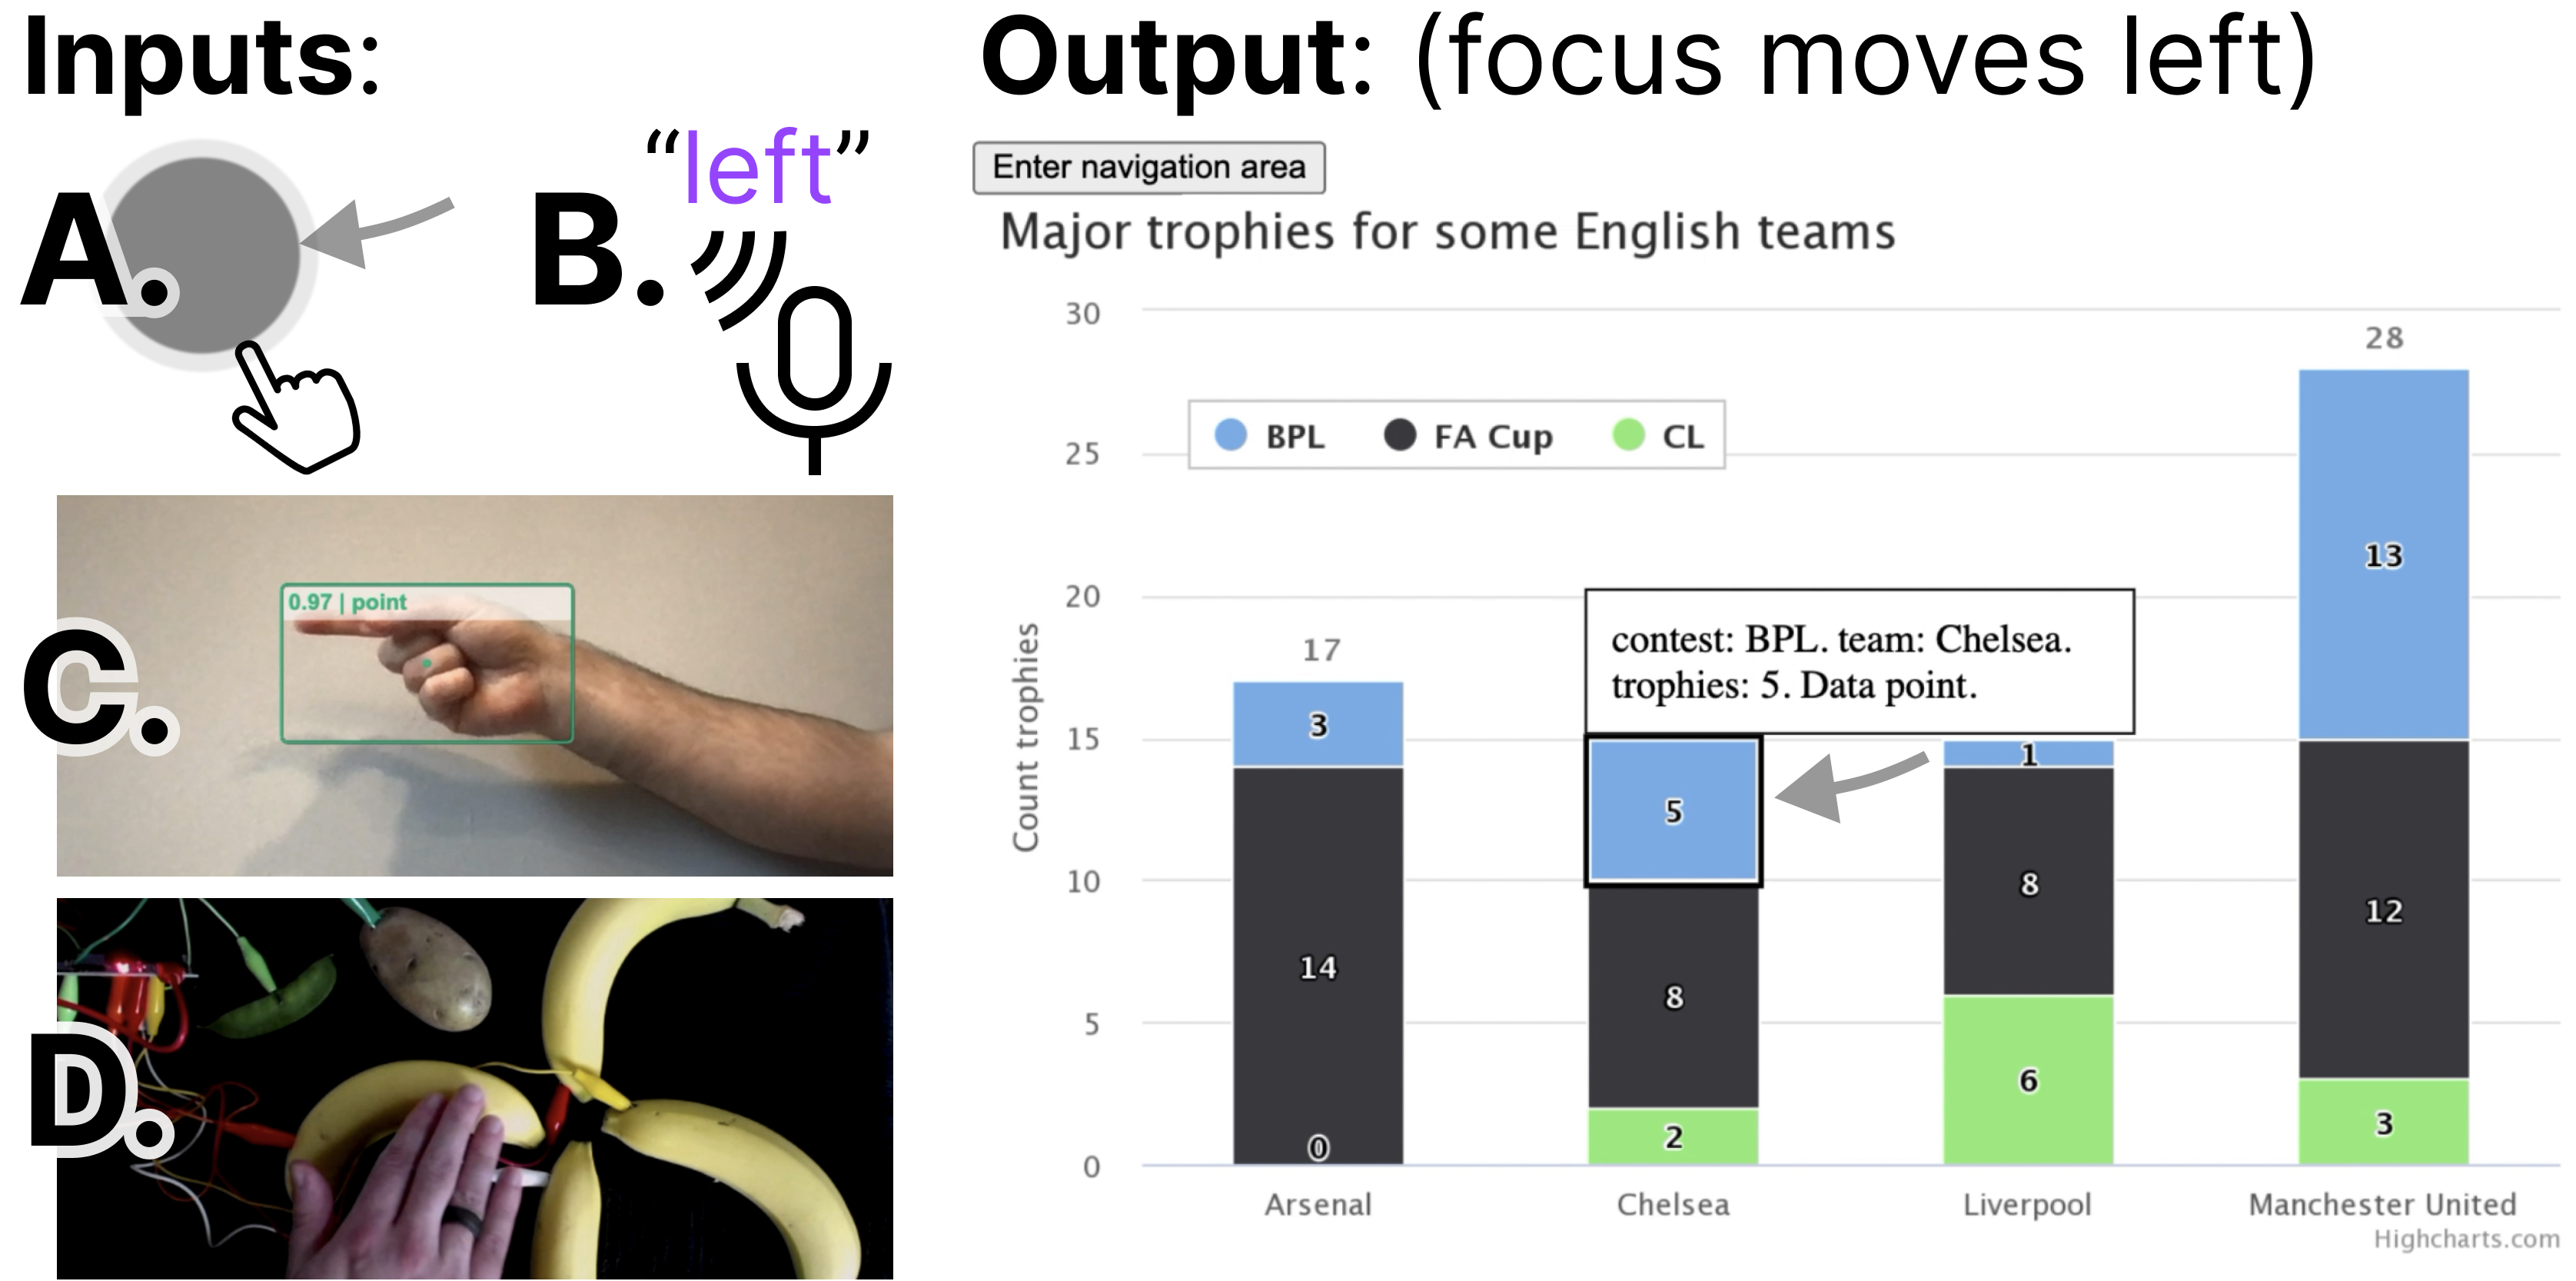
\includegraphics[width=\linewidth]{figures/inputs.png}
  \caption{An example navigation rule to move ``left'' can be called as a method by an event from any input modality. Some examples include common modalities such as touch swiping (\textbf{A}) or speaking ``left'' (\textbf{B}). This also includes advanced or future modalities such as gesture recognition (\textbf{C}) or touch-activated, fabricated interfaces (\textbf{D}).}
  % \Description{A mouse pointer is shown shaking over many data points that are very small while a touch hit area is shown over the same visualization, overlapping with many points at once.}
  \label{inputs}
\end{figure}
Navigation rules in Data Navigator (see \Cref{simple_movement} and \Cref{dynamic_movement}) are created alongside the node-edge structure. Edges reference rules for navigation. However, these rules are generic and agnostic to the specifics of input modalities and can be invoked as methods by virtually any detected user input event (see \Cref{inputs}).

Navigation rules are objects with a unique name, ideally as a noun or verb in natural language that refers to a direction or location, a movement direction (a binary used to determine moving towards the source or target of an edge), and optionally any known user inputs that activate that navigation, such as a keyboard keypress event name.

It is important for a system to abstract navigation events so that inputs can be uncoupled from the logic of Data Navigator. This allows higher level software or hardware logic to handle input validation while Data Navigator is just responsible for acting on validated input.

Later in our first case example (\Cref{section:raster}), we demonstrate an application that handles screen reader, keyboard, mouse and touch (pointer) swiping, hand gestures, typed text, and speech recognition input. Abstract navigation namespaces can be called by any of these input methods.

Additionally, since navigation rules are flexible, end users can also supply their own key-bind remapping preferences or input validation rules if developers provide them with an interface.

Because calling a navigation method is abstract, users can even supply events from their own input modalities as long they have access to either a text input interface or access to Data Navigator's navigation methods. Our demonstration material (in \Cref{section:raster}) also includes handling for DIY fabricated interfaces, which are important in accessibility maker spaces. We chose a produce-based interface~\cite{Rogers2014}, since it was an easy and low cost proof of concept.

We believe that enabling agnostic input provides a rich space for future research projects. In addition, browser addons and assistive technologies could both leverage this flexible interface for end users.

\begin{figure}[h]
  \centering
  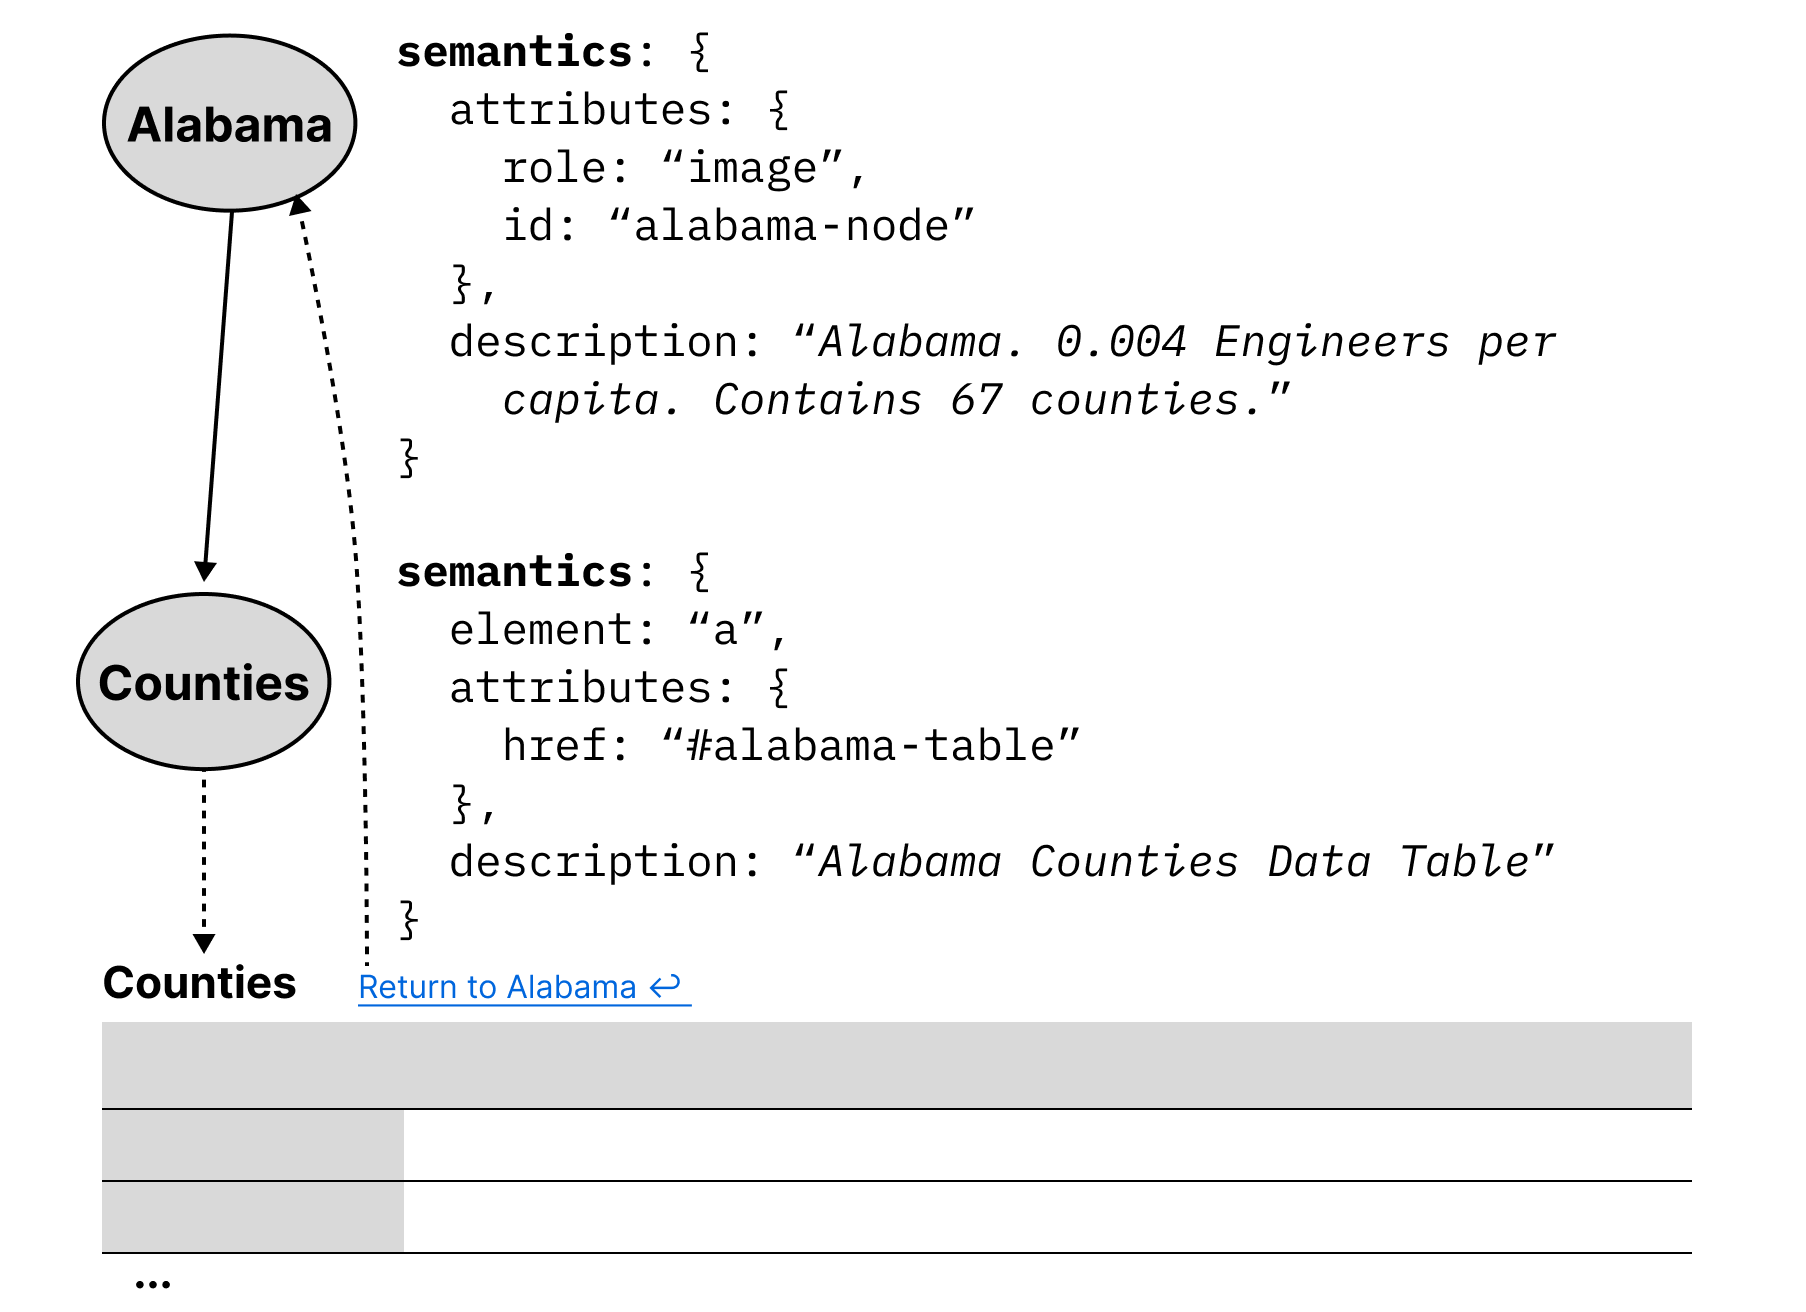
\includegraphics[width=12cm,height=12cm,keepaspectratio]{figures/semantics.png}
  \caption{An example of how navigation within Data Navigator could use semantic nodes as hyperlinks to provide access to other areas in an application. Alabama has a child node ``Counties'' which is a semantic HTML link element pointing to a table of counties, outside of Data Navigator's graph structure. A link is provided to return.}
  % \Description{A mouse pointer is shown shaking over many data points that are very small while a touch hit area is shown over the same visualization, overlapping with many points at once.}
  \label{semantics}
\end{figure}

\subsubsection{Discrete, sequential input opens new avenues}
The \textit{keyboard interface} is considered foundational for many assistive devices, which leverage this technology for discrete, sequential, non-pointer navigation and interaction~\cite{WAI2017Keyboard}. Desktop screen readers are the most common example of an assistive technology device that leverages the keyboard interface, however single or limited button switches, sip-and-puff devices, on-screen keyboards, and many refreshable braille displays do as well. Support for the keyboard interface by default in turn provides all discrete, sequential input devices with access as well.

However by basing Data Navigator's foundational infrastructure on a keyboard-like modality, this also provides designers and developers new avenues to imagine how existing direct, pointer-based, or continuous inputs can map to discrete, sequential navigation experiences.

For example, with mobile screen readers this already happens: screen reader users swipe and tap on their screen to sequentially navigate, but the exact pixel locations of their swiping and tapping generally does not matter. Their current focus position is discrete and determined by the screen reader software.

Data Navigator therefore allows for many new possibilities. One possibility is that sighted mouse and touch users may now also swipe their way through dense plots or use small interfaces (such as on mobile devices) that may otherwise be too hard to precisely tap. Data Navigator optionally removes the accessibility barriers sometimes posed by precision-based input in visualizations.

Data Navigator does not have to be in conflict with precision-based input, either. A discrete, sequential navigation infrastructure can be used in tandem with precision-based pointer events as well as instant access when coupled with voice commands and search features.

\subsection{Rendering}
\begin{figure}[h]
  \centering
  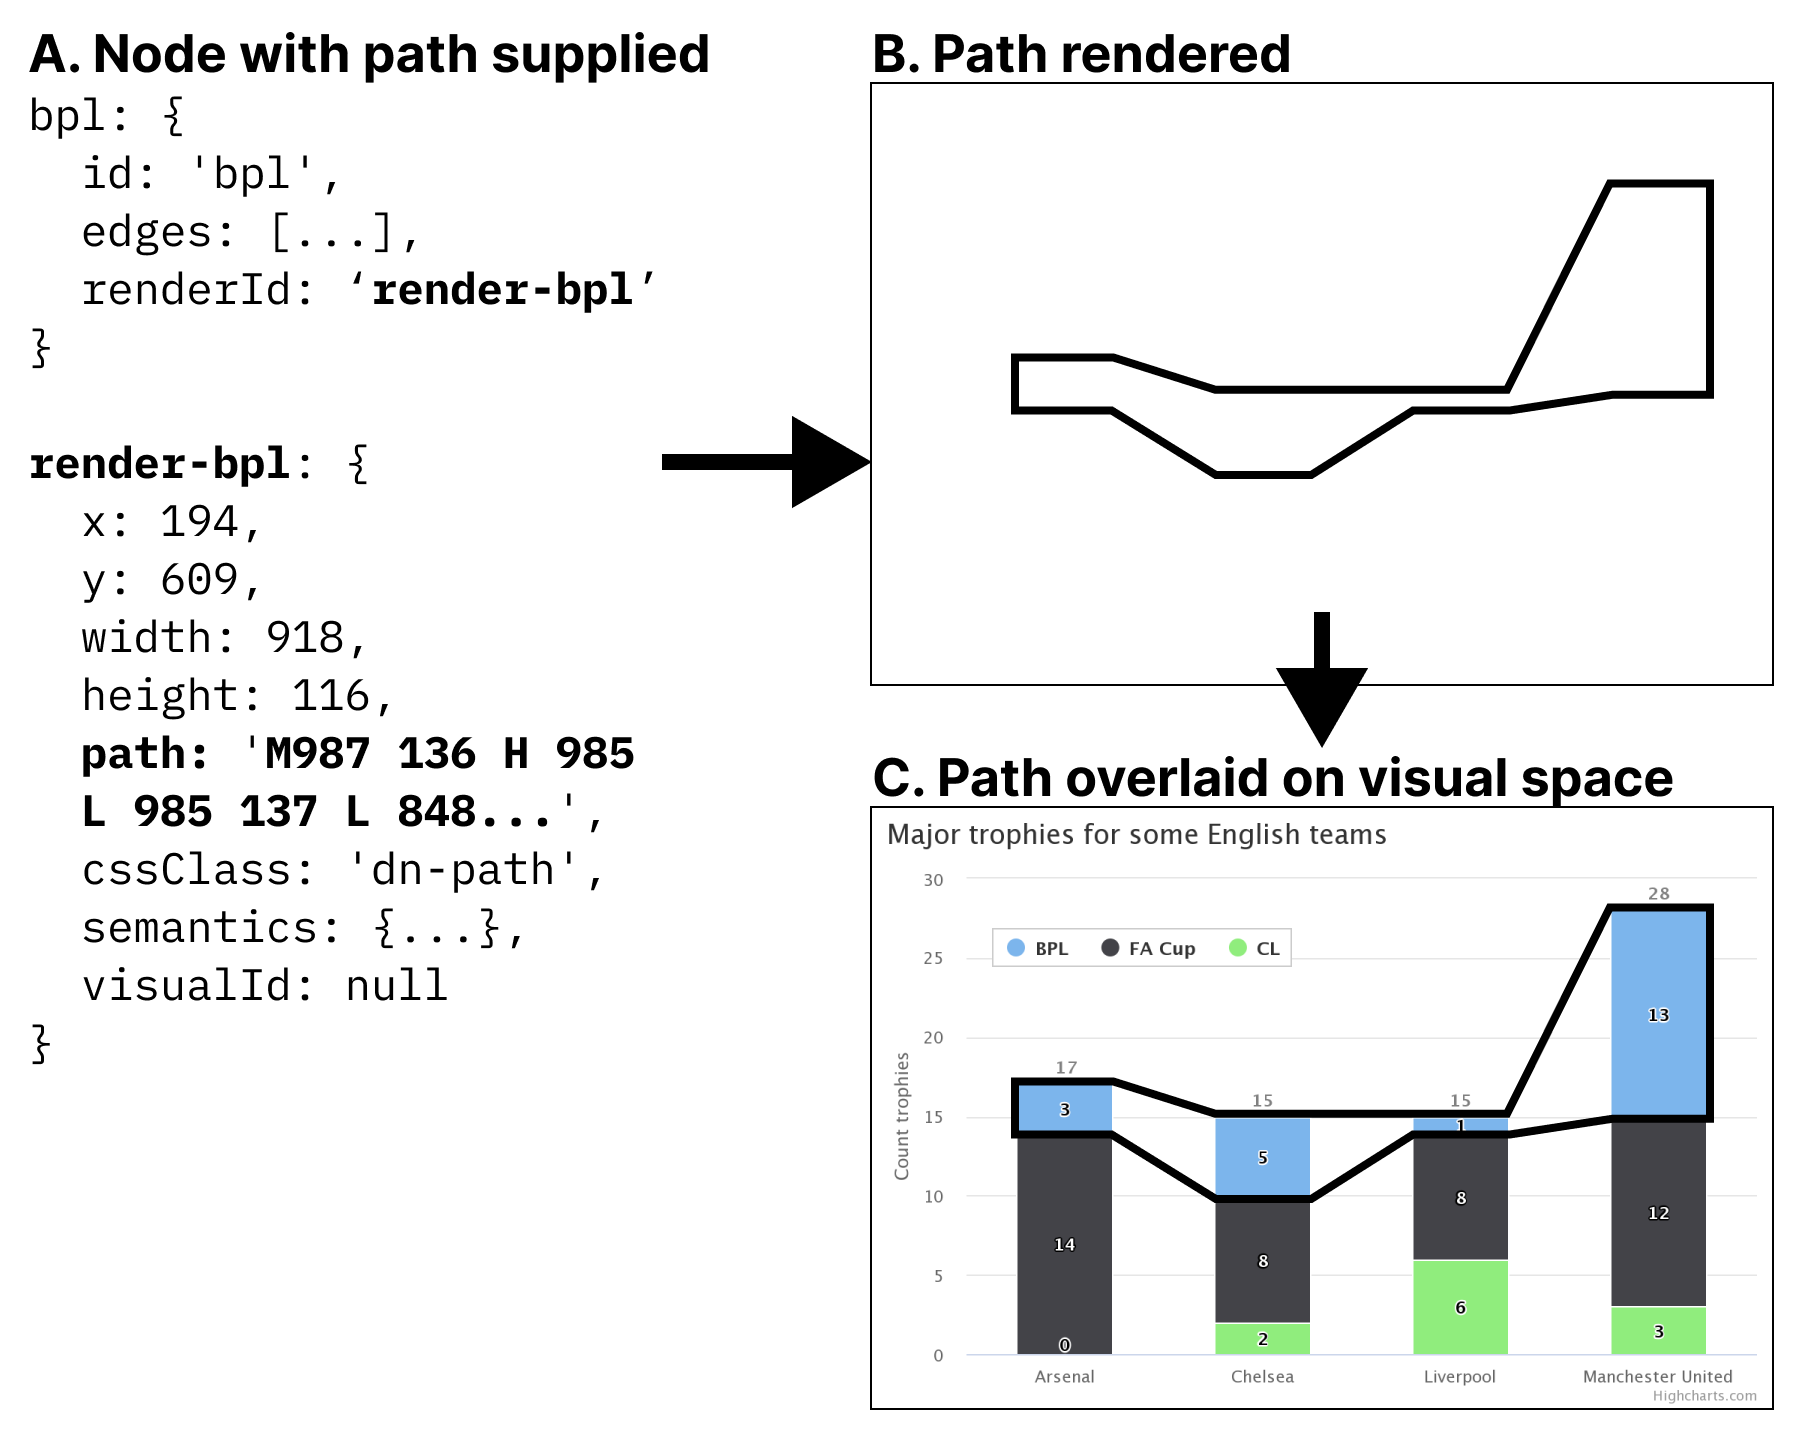
\includegraphics[width=0.65\linewidth]{figures/path.png}
  \caption{\textbf{A.} The data specified for a node with a reference to separate data that is used to render that node. \textbf{B.} The node will render as a path at the specified Cartesian coordinates. \textbf{C.} This rendered node may then be placed over a visual.}
  % \Description{A mouse pointer is shown shaking over many data points that are very small while a touch hit area is shown over the same visualization, overlapping with many points at once.}
  \label{path}
\end{figure}

\subsubsection{Flexible node semantics provide freedom}
Nodes in Data Navigator are semantically flexible. This is because the marks in a data visualization may represent many things, that are either dependent on the data or the user interface materials.

\begin{figure*}[h]
  \centering
  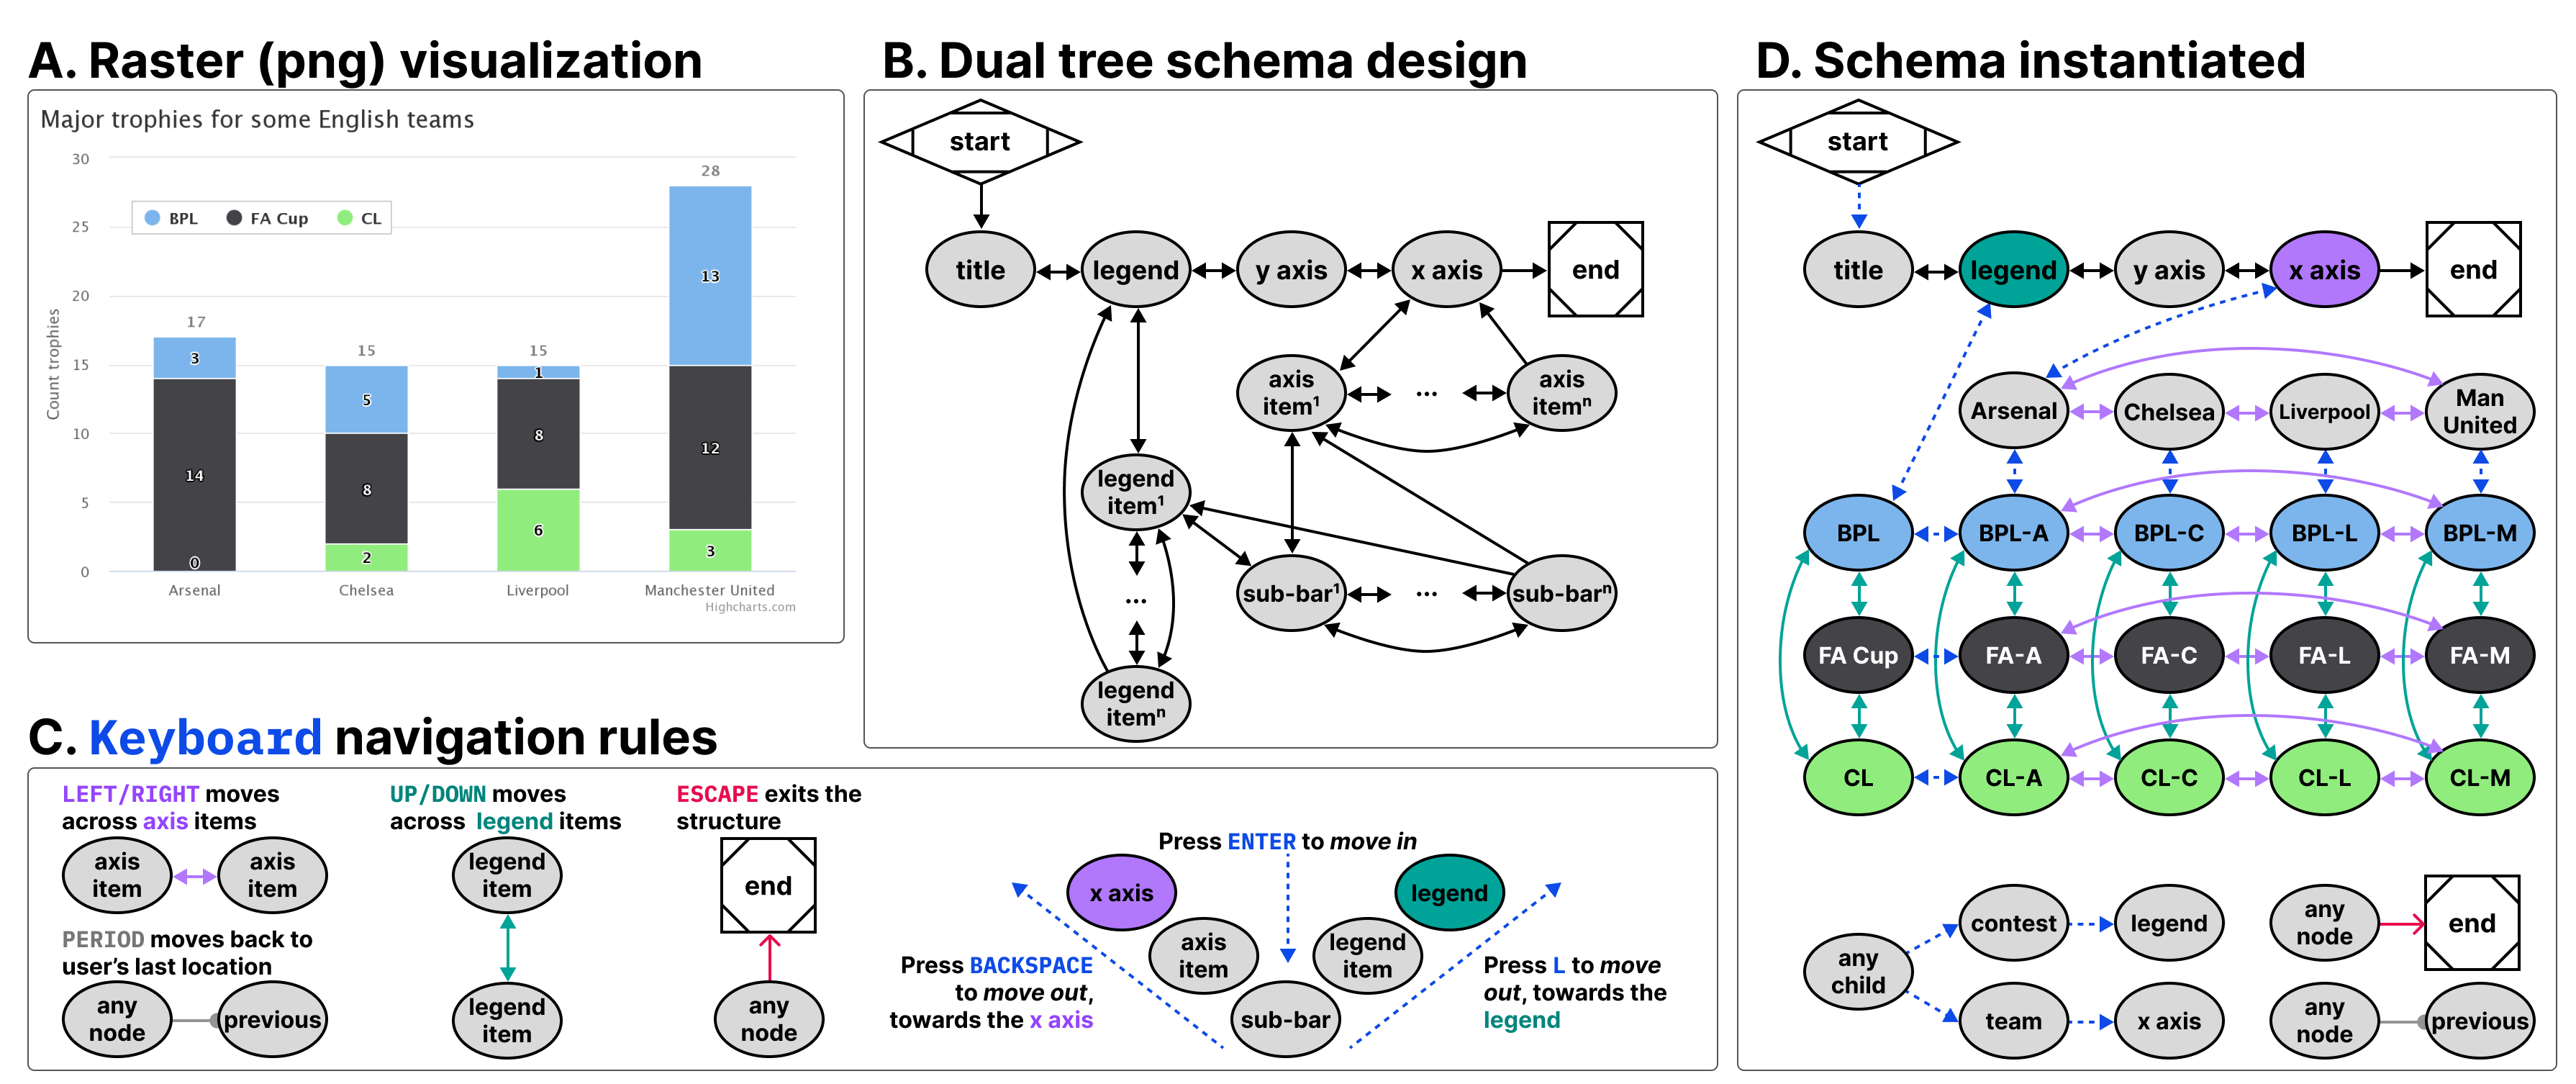
\includegraphics[width=\textwidth]{figures/static.png}
  \caption{\textbf{A.} A raster (png) visualization of a stacked bar chart showing how 4 English teams performed across 3 major trophy contests. \textbf{B.} An example navigation schema that allows children nodes to have 2 parents (two tree structures intersecting), one for contests and one for teams. \textbf{C.} An example of Data Navigator's navigation logic abstraction, which allows edge types to have programmatic sources, targets, and rules, such as a single rule that gives all nodes a edge to exit the visualization. \textbf{D.} An instantiation of the schema, showing all corresponding rendered nodes and their edge types according to the schema design and navigation rules.}
  % \Description{A mouse pointer is shown shaking over many data points that are very small while a touch hit area is shown over the same visualization, overlapping with many points at once.}
  \label{static}
\end{figure*}

Since our toolkit implementation is in JavaScript and HTML, our map example from \Cref{map} might use image semantics for states, alongside a description of the data relevant to that node. However since semantics are flexible in this way, Data Navigator could also be used to integrate into a larger ecosystem, with nodes rendered as hyperlinks to tables or other elements such as in \Cref{semantics}.

The concept of using node-edge graphs can even extend to have ``nodes'' that are entirely different parts of a document or tool, as well as integrated into the explicit structure provided by Data Navigator. In some accessibility toolkits, nodes are geometries without functional semantics~\cite{Satyanarayan2017VegaLite} or list items nested within lists~\cite{Blanco2022olli}. But in Data Navigator, nodes can semantically be buttons, links, or any HTML element. Interactive data visualizations sometimes demand more flexible node semantics than geometries or lists.

\subsubsection{Loose-coupling to visuals enables expressiveness}

One of the most significant technical limitations of existing data visualization toolkits with regards to accessibility is that they rely on visual substrate, or visual materials, in order to produce data visualizations. In the case of static, raster images such as png files or WebGL and canvas elements on the web, there are no interface properties at all exposed to screen readers for programmatic exploration and interaction.

If raster images are used, they generally cannot be changed after rendering. However, according to web accessibility standards, elements must have a visual indicator provided when focused~\cite{WAI2016Focus}.

Since Data Navigator navigates using focus, an indicator must be rendered alongside the node semantics. But \textit{what} is focused visually and \textit{where} it is depends on different design needs.

In \textit{Visa Chart Components}, chart elements can be \textit{selected}, so the focus indication is visible over the existing elements in the chart space. The design choice to have interactive visual elements located within a chart or graph is also common in other toolkits that provide accessible focus indication, such as \textit{Highcharts}, \textit{PowerBI}, and \textit{SAS Graphics Accelerator}.

However, some visualization toolkits create accessible structures entirely uncoupled from visual space~\cite{Blanco2022olli}, so focus indication is provided beneath or beside the chart, not over it.

Due to the different ways that accessibility might be provided, Data Navigator enables developers to have complete control over the rendering of which focus elements they want, in what styling, and where. This can accommodate both un-coupled and visually-coupled approaches to focusing and more.

Data Navigator's focus is \textit{uncoupled} by default and may even be used independent of any existing graphics at all. Rendering information may be passed to Data Navigator for it to render (like in \Cref{path}) or developers can provide their own rendered elements and simply use Data Navigator to move between them.

Because of Data Navigator's approach to rendering focusable elements, designers and developers can provide fully customized annotations, graphics, text, or marks that may not be not part of the original visual space or elements. One example of this might be adding an outlined path to a collective cross-stack group of bars in a stacked bar chart (see \Cref{path}).

Loose-coupling in this way provides robust flexibility to designers and developers to handle navigation paths and stories through a data visualization, even in bespoke or hand-crafted ways.

\subsubsection{On-demand node rendering is efficient}
Practitioners care about performance and so do users. Practitioner toolkits often focus on lazy-loading techniques where accessibility elements are rendered on-demand rather than all in-memory up front~\cite{Elavsky2021Method,Zong2022Rich,Blanco2022olli}.

Data Navigator's nodes are rendered \textit{on-demand} by default. Data Navigator only renders the node that is about to be focused by the user and after it is focused, the previously focused node is deleted from memory. This technique has advantages in cases where datasets are large or users have lower computational bandwidth available. However, there are cases where practitioners may want to render all of Data Navigator's structure in memory, such as server-side rendering or equivalent. Pre-rendering may be optionally enabled.

\section{Case Examples with Data Navigator}
We built example prototypes using our JavaScript implementation of Data Navigator, available open source at our \href{https://github.com/cmudig/data-navigator}{GitHub repository}.

Our first two prototype case examples represent some of the most powerful parts of Data Navigator as a system while reproducing known and effective data navigation patterns from existing industry and research projects. We provide a final case example as a co-design session that demonstrates how Data Navigator may be used to rapidly build new designs.

\subsection{Augmenting a Static, Raster Visualization}
\label{section:raster}
The first case example (shown in \Cref{static}) builds on an online JavaScript visualization library, \textit{Highcharts}. \textit{Highcharts} already provides relatively robust data navigation handling out of the box for screen reader, keyboard, and even voice recognition interface technologies, such as \textit{Dragon Naturally Speaking}. However, these capabilities are only provided when the chart is rendered using SVG. Developers have several other rendering options available, including WebGL, which is significantly more efficient~\cite{HighsoftBoost}. We wanted to demonstrate that Data Navigator can provide a navigable data structure even if the underlying visualization is a raster image.

For our case example, we exported a png file using the built in menu of a sample stacked bar chart retrieved from their online demos~\cite{HighchartsStacked}. We selected a stacked bar chart because it allows us to demonstrate how two tree structures may interact and share the same children nodes.

We recorded the data and hand-created all of the geometries and their spatial coordinates using \textit{Figma}, by tracing lines over the raster image's geometries (see samples of the data and traced geometries in \Cref{path}). While this method was efficient for building an initial prototype, \Cref{section:ecosystem} engages deterministic methods for extracting and producing the nodes, edges, and descriptions required by Data Navigator automatically and at scale.

The visualization we selected represents 4 English football teams, \textit{Arsenal, Chelsea, Liverpool,} and \textit{Manchester United} and how many trophies they won across 3 contests, \textit{BPL, FA Cup,} and \textit{CL}.

We chose a schema design that arranged the \textit{contests} to be navigable across one dimension of movement (\textit{up} and \textit{down}) while the \textit{teams} are navigable across a perpendicular dimension of movement (\textit{left} and \textit{right}). This 2-axis style of navigation is used by \textit{Highcharts} (when rendering as SVG) and \textit{Visa Chart Components}. We also chose these directions because it is coincidental that their visual affordance is closely coupled with the navigation design (the x axis is ordered \textit{left} to \textit{right} and since the bars are stacked, \textit{up} and \textit{down} can move within the stack). These directions can also be applied to the axis categories and legend categories as well, moving \textit{left} and \textit{right} across the entire \textit{team's} stacks or up and down across the entire \textit{contest's} groupings.

Using a keyboard, a user might enter this schema and navigate to the legend, where they could press \textit{Enter} to then focus the legend's first child, pictured in \Cref{path}. Pressing up or down navigates in a circular fashion among the \textit{contest} groupings. Pressing \textit{Enter} again then focuses the first child element of that \textit{contest}, all of which are in the \textit{Arsenal} group, since it is the first group along the x axis. A user can then navigate \textit{up, down, left,} and \textit{right} among children. Pressing \textit{L Key} moves the user back up towards the contest while pressing \textit{Backspace} moves the user up towards the x axis. The x axis and \textit{team} groupings represent the second tree which intersects the first (the \textit{contests}).

Our first case example includes handling for additional input modalities beyond screen readers and keyboards, including a hand gesture recognition model, swipe-based touch navigation, and text input (which can be controlled using voice recognition software).

\subsubsection{Discussion}
Our first case example demonstrates several of the most important capabilities of Data Navigator, namely that practitioners can add accessible navigation to previously inaccessible, static, raster image formats and that a wide variety of input modalities are supported easily.

Widely-used toolkits like \textit{Vega-Lite}, \textit{Highcharts}, and \textit{D3}~\cite{Bostock2011D3} allow practitioners to choose SVG and canvas-based rendering methods. Data Navigator's affordances help overcome the lack of semantic structure in canvas-based rendering, allowing developers to take advantage of its processing and memory efficiency.

Notably in addition to these capabilities, the visual focus highlighting added was entirely bespoke (as in~\Cref{path}) and the navigation paths through the visual were based on our design intentions, not an extracted view or underlying architecture such as render order. This demonstrates that our system provides a significant degree of freedom and control for designers and developers.

As a final discussion point, the resulting visualization contains no automatically detectable accessibility conformance failures according to the W3C's Web Accessibility Initiative's accessibility evaluation tool, \textit{WAVE}~\cite{WebAIMWAVE}. It is important for any technology developed to also meet minimum requirements for accessibility~\cite{Lundgard2019Sociotechnical,Lundgard2022Accessible,Zong2022Rich,Elavsky2022Chartability}, even when following best-practices and research.

\subsection{Building Data Navigation for a Toolkit Ecosystem}
\label{section:ecosystem}
\begin{figure}[h]
  \centering
  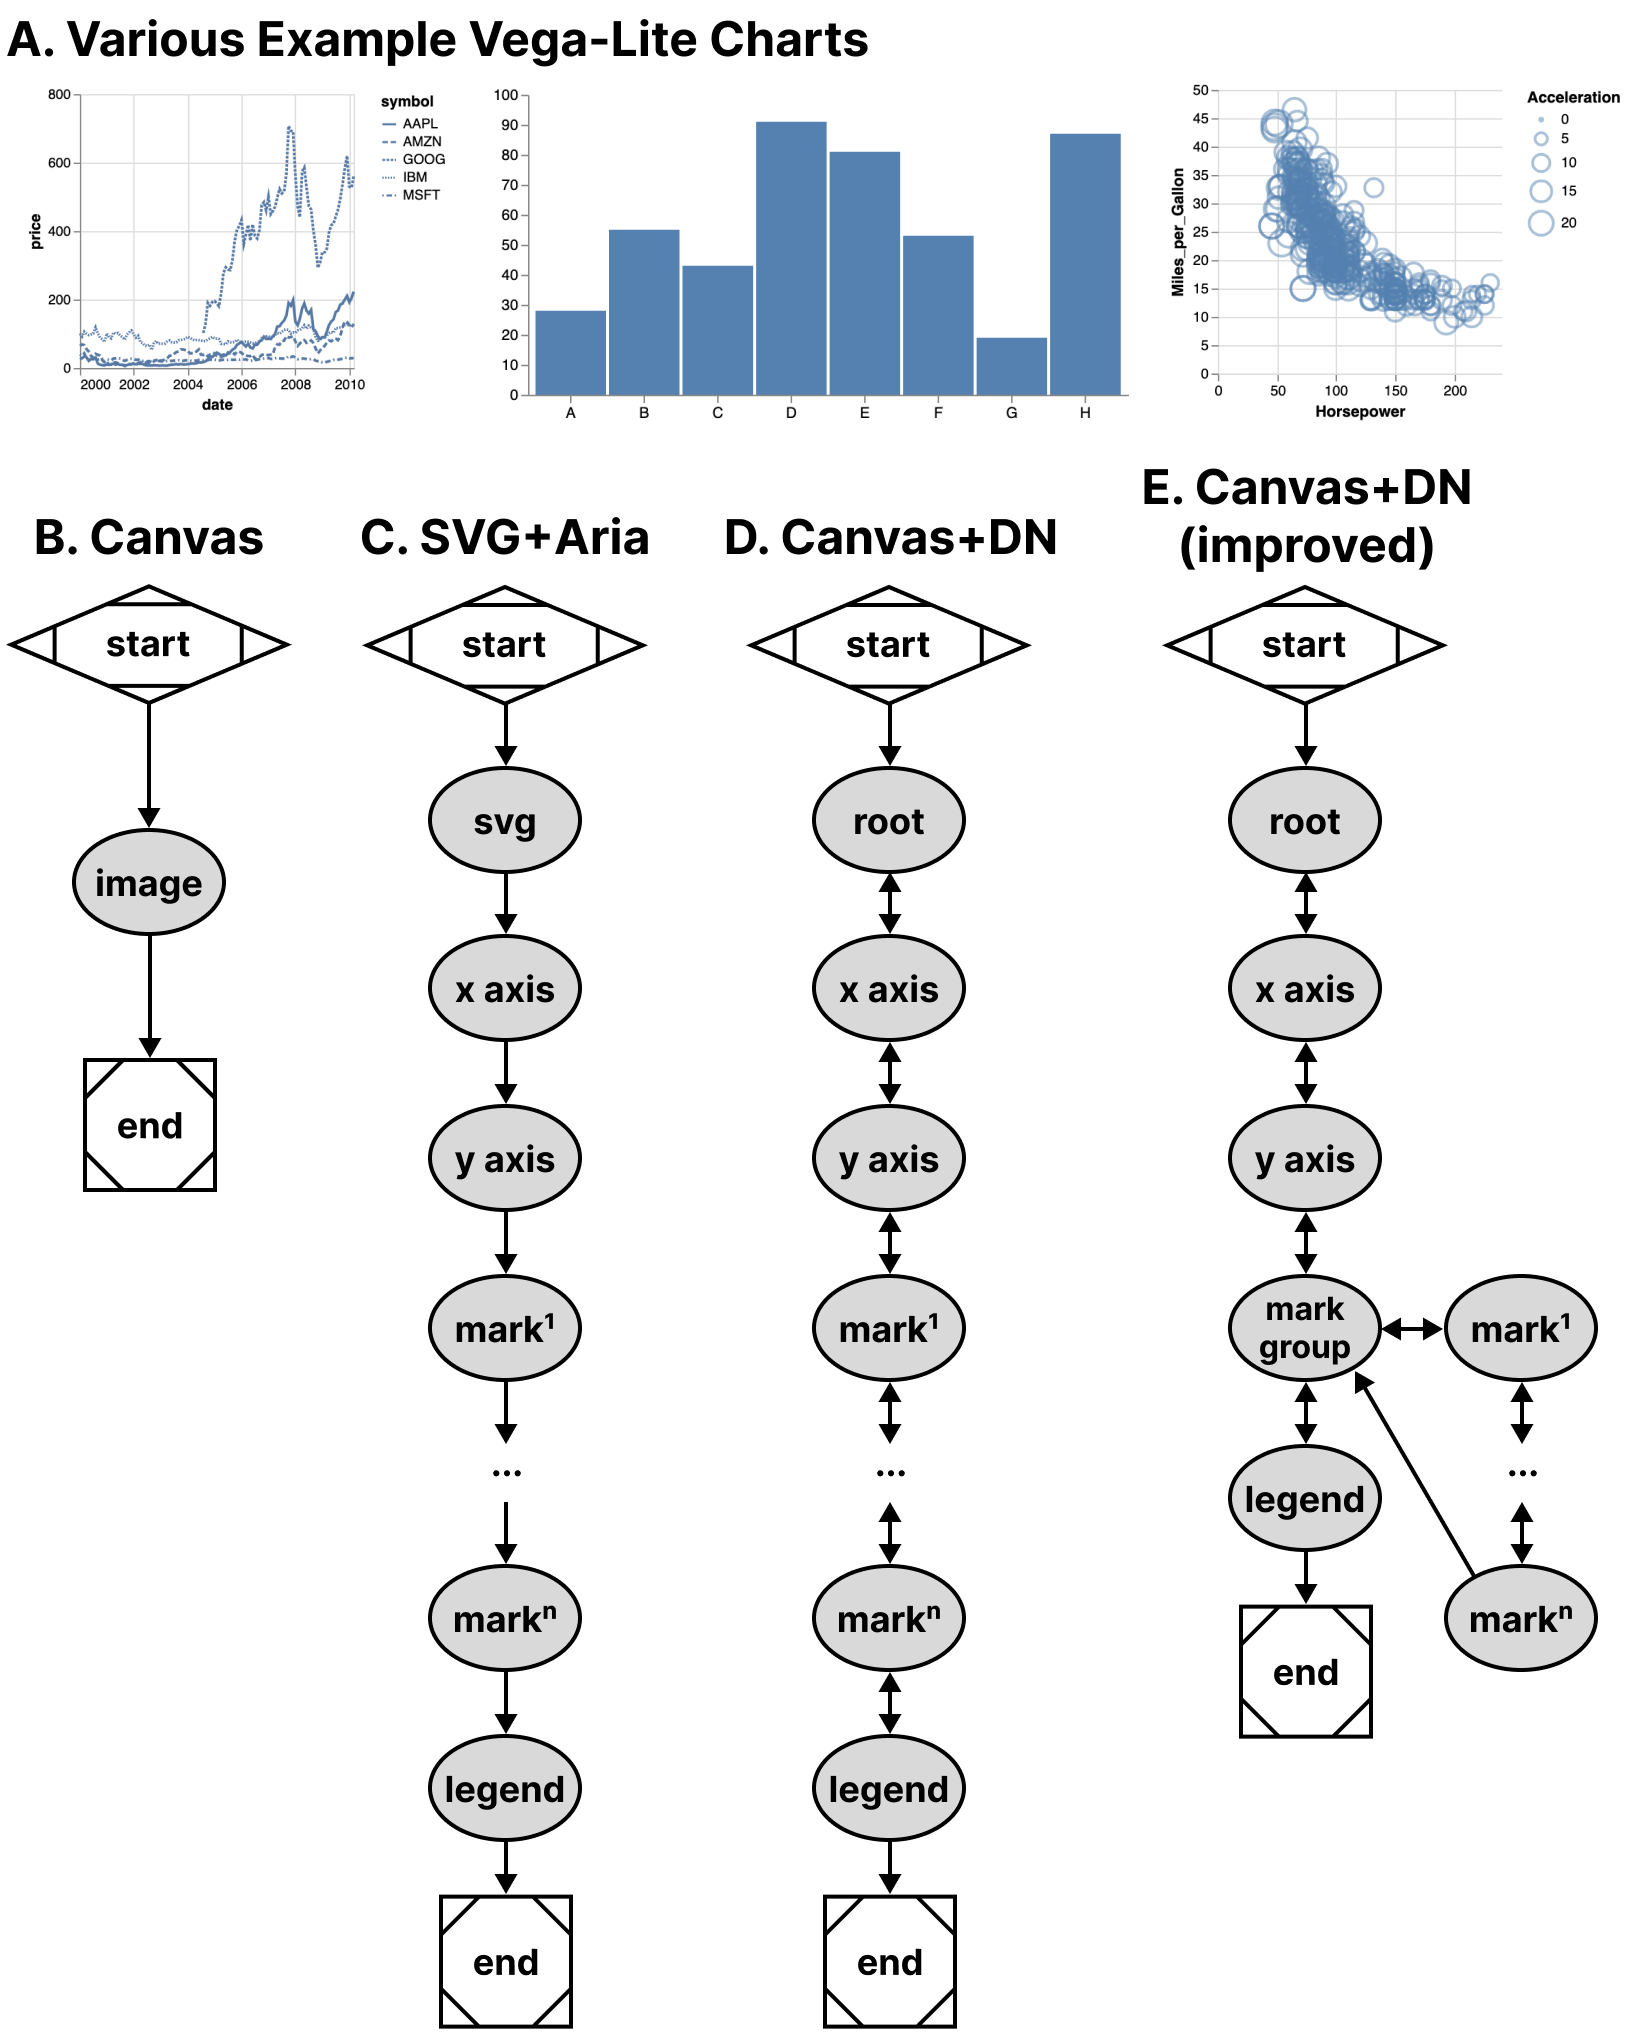
\includegraphics[width=10cm,height=10cm,keepaspectratio]{figures/vega-lite.png}
  \caption{\textbf{A.} Various charts from \textit{Vega-Lite} share the same general structures with each other when rendered using canvas (\textbf{B}) or SVG (\textbf{C}). \textbf{D.} With Data Navigator, we replicated the existing SVG navigation pattern (\textbf{C}) but used a canvas-based rendering for the visualization. \textbf{E.} We also improved the navigation scheme to nest marks within a mark group to allow users to skip them, if needed.}
  % \Description{A mouse pointer is shown shaking over many data points that are very small while a touch hit area is shown over the same visualization, overlapping with many points at once.}
  \label{vega-lite}
\end{figure}

Our second case example, shown in \Cref{vega-lite}, builds on \textit{Vega-Lite}. As shown in \Cref{existing}, \textit{Vega-Lite} offers basic screen reader navigation but provides no navigation at all when rendered using canvas.

While it might be a tedious design choice to allow every mark in a visualization to be serially accessible to screen reader users, we nevertheless set out to build a generic ingestion function that would take a \textit{Vega-Lite View} object and deterministically recreate their existing SVG navigation structure in Data Navigator. This way users would have the same experience between SVG rendered charts and all current and future rendering options that \textit{Vega-Lite} offers to developers. 

Notably, \textit{Vega-Lite} does not explicitly manipulate the navigation order at all when rendering with SVG. ARIA is simply provided to allow screen reader users to access each mark in the visualization in the order the mark appears in the DOM (which is the order it was rendered). The legend appears after the marks in our schema for this reason because \textit{Vega-Lite} renders the legend after marks. This choice of ordering is for visual reasons: z-axis placement is currently based on render order in SVG and \textit{Vega-Lite} wants their legend visually on top of the rendered marks.

In addition to mimicking their existing SVG navigation strategy, we also created a way to nest all of the marks within a group so that users can skip past them and drill in on-demand, which is a valuable pattern when dealing with situations where providing a mark-level fidelity of information may not be relevant to a user's needs by default~\cite{Shneiderman2003Eyes,Zong2022Rich}.

In order to deterministically supply Data Navigator with accurate information about any given \textit{Vega-Lite} visualization, we built 3 functions: one that takes a \textit{Vega-Lite View} as input and extracts meaningful nodes, one that produces edges based on those nodes, and one to describe our nodes in a meaningful way for screen reader users. These generic functions technically work on all existing \textit{Vega-Lite} charts, however some are more useful out of the box than others due to the type of marks involved.

\subsubsection{Discussion}
This case example demonstrates that ecosystem-level remediation and customization is not only possible for toolkit builders but Data Navigator offers robust potential. Data Navigator's structure, input, and rendering capabilities are all flexible and can be adjusted to suit the needs of a specific toolkit's design  and intended use.

Many visualization libraries may not even provide screen reader accessible SVG using ARIA-based approaches but do have a consistent underlying architectural pattern. Some libraries have a consistent method for converting data into visual formats, readable text labels, and interaction logic. Strong contenders would be visualization libraries popular in online, web-based data science notebooks like \textit{ggplot2} in R or \textit{matplotlib} for Python, which typically only render rasterized pngs or semanticless SVG.

Toolkits with consistent underlying architecture would allow toolkit developers, not just developers who \textit{use} toolkits, to remediate and customize their navigation accessibility using a generic approach.

Enabling accessibility at the toolkit level allows all downstream use of that tool to have better defaults, options, and resources available for building more accessible outcomes for end users.

Many libraries and toolkits provide users with a level of functional defaults and abstract conciseness so that users don't have to worry about low-level geometric considerations~\cite{Satyanarayan2017VegaLite}.

Data Navigator allows toolkits developers to also provide their users with abstractions and defaults for accessibility that make sense for their ecosystem.

Despite our schema recreating a screen reader experience based on SVG (and improving it), Data Navigator's additional features also apply: users are able to leverage a much wider array of input modalities.

\textit{Vega-Lite} provides many ways to make marks clickable and even perform complex actions using mouse-based input. While Data Navigator does not engage accessible brush and drag-based inputs, it does provide keyboard-only access by default, which can be used to make events previously only accessible to mouse clicking available to many other technologies. This is an improvement over \textit{Vega-Lite}'s SVG + ARIA rendering option.

When measuring performance across test datasets containing 406 and 20,300 data points in a scatter plot, Data Navigator increases initialization time by $\sim$0.45 to $\sim$1.5ms respectively. Our extraction functions specific to \textit{Vega-Lite} increase initialization between $\sim$4.8 and $\sim$8.5ms respectively. Given that our benchmark testing for \textit{Vega-Lite's} SVG rendering initialized in $\sim$1,800ms for 20,300 data points and canvas in $\sim$700ms, we do not anticipate that Data Navigator will have a negative impact on performance in most visualization contexts.

\subsection{Co-designing Novel Data Navigation Prototypes}
\label{section:codesign}
\begin{figure}[ht]
  \centering
  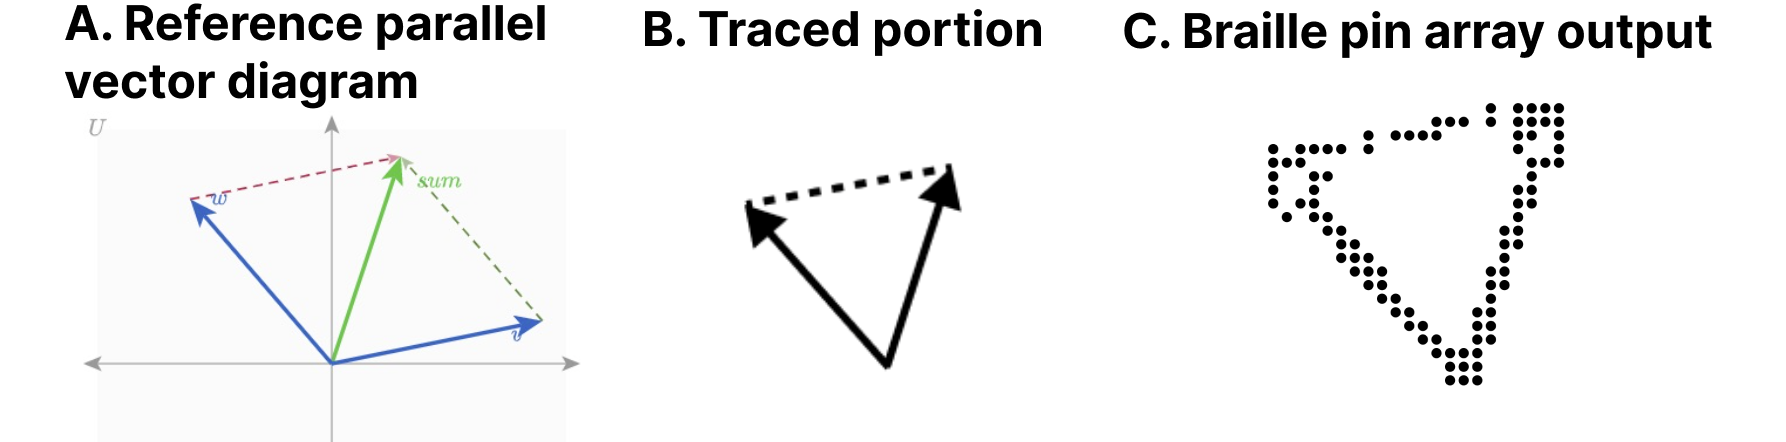
\includegraphics[width=\linewidth]{figures/braille.png}
  \caption{Our material preparation process involved taking a reference (\textbf{A}), tracing it (\textbf{B}), and rendering it on a tactile display (\textbf{C}).}
  % \Description{A mouse pointer is shown shaking over many data points that are very small while a touch hit area is shown over the same visualization, overlapping with many points at once.}
  \label{braille}
\end{figure}
Recent projects in accessible data navigation have involved extensive co-design work with people with disabilities, ranging on the magnitude of months with as many as 10 co-designers at a time~\cite{Lundgard2019Sociotechnical,Lundgard2022Accessible,Zong2022Rich,Thompson2023Chart}.

However many visualization experiences may be authored in smaller scales, with fewer designers, and less time such as the development of a prototype or demonstration of an emerging idea. In practical or industry contexts, co-design sessions (and design sessions in general) may be much shorter. The goal of these co-design sessions is simply to create an artifact with the artifact's intended users.

Since our paper is contribution towards practical outcomes, we simulated a light co-design session with the aim of producing low-fidelity prototypes of novel data interaction patterns.

\subsubsection{Co-design Session Methods and Setup}
\begin{figure}[h]
  \centering
  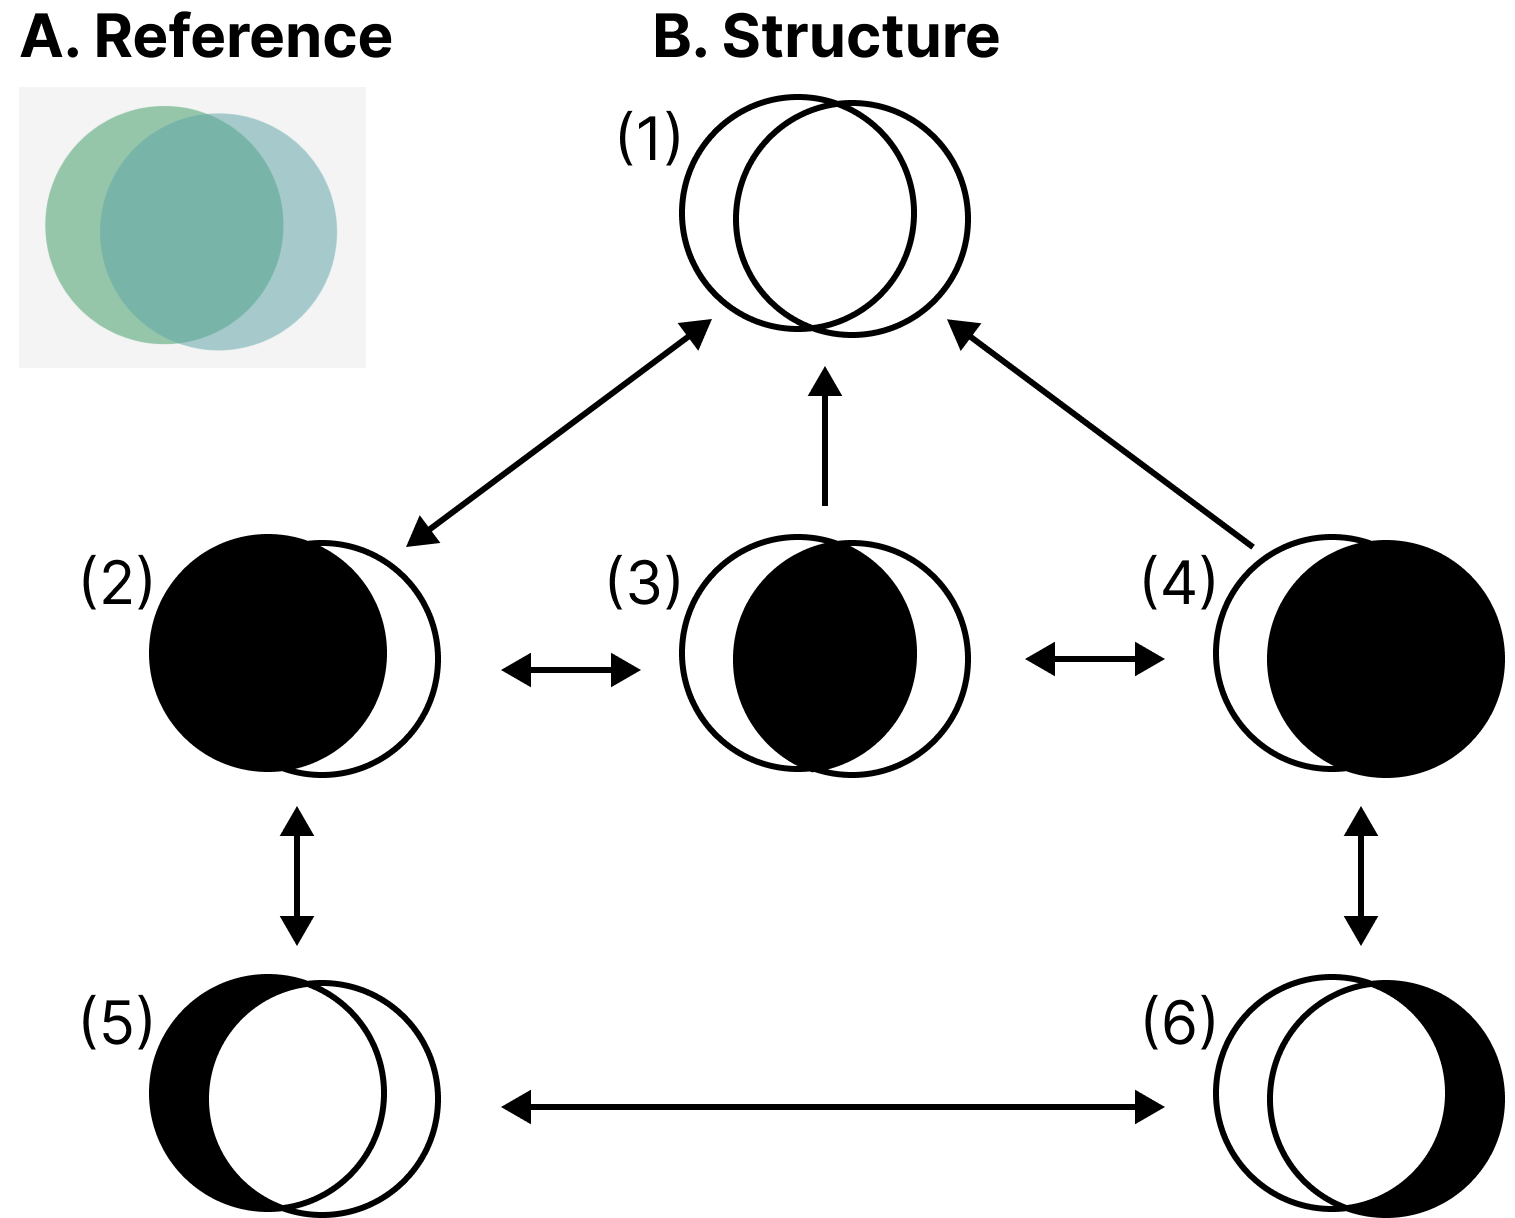
\includegraphics[width=0.65\linewidth]{figures/sets.png}
  \caption{\textbf{A.} A reference image from \textit{Penrose} of a set diagram containing two sets intersecting. \textbf{B.} A diagram of our proposed structure, with three levels of information.}
  % \Description{A mouse pointer is shown shaking over many data points that are very small while a touch hit area is shown over the same visualization, overlapping with many points at once.}
  \label{sets}
\end{figure}

Authors Frank Elavsky (sighted) and Lucas Nadolskis (blind) set out with the goal of developing screen-reader friendly prototypes that can explore geometric and mathematical models produced by the math diagramming tool \textit{Penrose}~\cite{Ye2020Penrose}.

Nadolskis is a neuroscience engineer who is a native screen reader user and uses both mathematical concepts as well as data-related tasks in his research. Elavsky proposed a series of possible math-based visualization types produced by \textit{Penrose} to build prototypes for, and Nadolskis selected \textit{set} and \textit{vector} diagrams as the two worth exploring first. The justification for this selection is that understanding these two concepts is important for work in data science, programming, and more advanced math concepts.

In particular we grounded the context of our contribution in a hypothetical classroom setting, where a screen reader user who is a student will have access to the equations in both raw text and \textit{MathJax}. We want to provide an experience that does not replace the existing resources screen reader users have to learn in classrooms but rather supplement.

At our disposal for our co-design session was a \textit{Dot Pad}~\cite{Dot2020Dot}, which is a refreshable tactile braille display. Our \textit{Dot Pad} enabled Elavsky to produce something visual and then translate it into the display for Nadolskis. Similar to de Greef \ea~\cite{deGreef2021Interdependent}, we used a tactile interface as an intermediary to help us get a shared sense of the meaningful spatial features of our figures.

Elavsky started with a reference diagram and then traced a wide variety of every possible node that might be worth navigating to in the diagram (see \Cref{braille}).

We selected which nodes were most important in each diagram, how to navigate between them, and how we wanted to render their visuals and semantics.

The selection of our problem space, scope of solutions, context of contribution, general discussion, and preparation of materials took approximately 12 hours of work over 2 weeks. The exploration of our prototype design space for our 2 prototypes took 1 hour. Building the prototypes took 2 hours.

\subsubsection{Creating a Navigable Set Diagram}

Our first prototype was a set diagram (see~\Cref{sets}). For our structure, we decided that it has 3 important semantic levels: the high level, the inclusion level, and the exclusion level. The inclusion level is first and the siblings are all sets or subsets that include other sets. The exclusion level is beneath and contains sets or subsets that are exclusive to the sets they belong to, which are accessed by drilling down from a set. 

Our schema design starts with a user encountering the root level (1) and may optionally drill in to the first child of the next level (2) using the \textit{Enter} key. The user may navigate siblings at this level using \textit{right} and \textit{left} directions, but this level is not circular (like in \Cref{static}) to maintain the spatial relationships. The user may drill in on either set again to view the non-intersecting portion of that set. Any node can drill up, towards the root, using \textit{Escape} or \textit{Backspace}.

% \textbf{Rendering.} The following descriptions correspond to the numbered nodes in \Cref{sets}:
% \begin{enumerate}
%   \itemsep-0.4em
%   \item “Set A intersects Set B. Spatial view.”
%   \item “Set A, count: 10. Contains 1 intersection and 1 non-intersecting subset.”
%   \item “Set A and B intersection, count: 7.”
%   \item “Set B, count: 10. Contains 1 intersection and 1 non-intersecting subset.”
%   \item “Set A non-intersecting subset, count: 3.”
%   \item “Set B non-intersecting subset, count: 3”
% \end{enumerate}

\subsubsection{Creating a Navigable Parallel Vectors Diagram}
\begin{figure}[h]
  \centering
  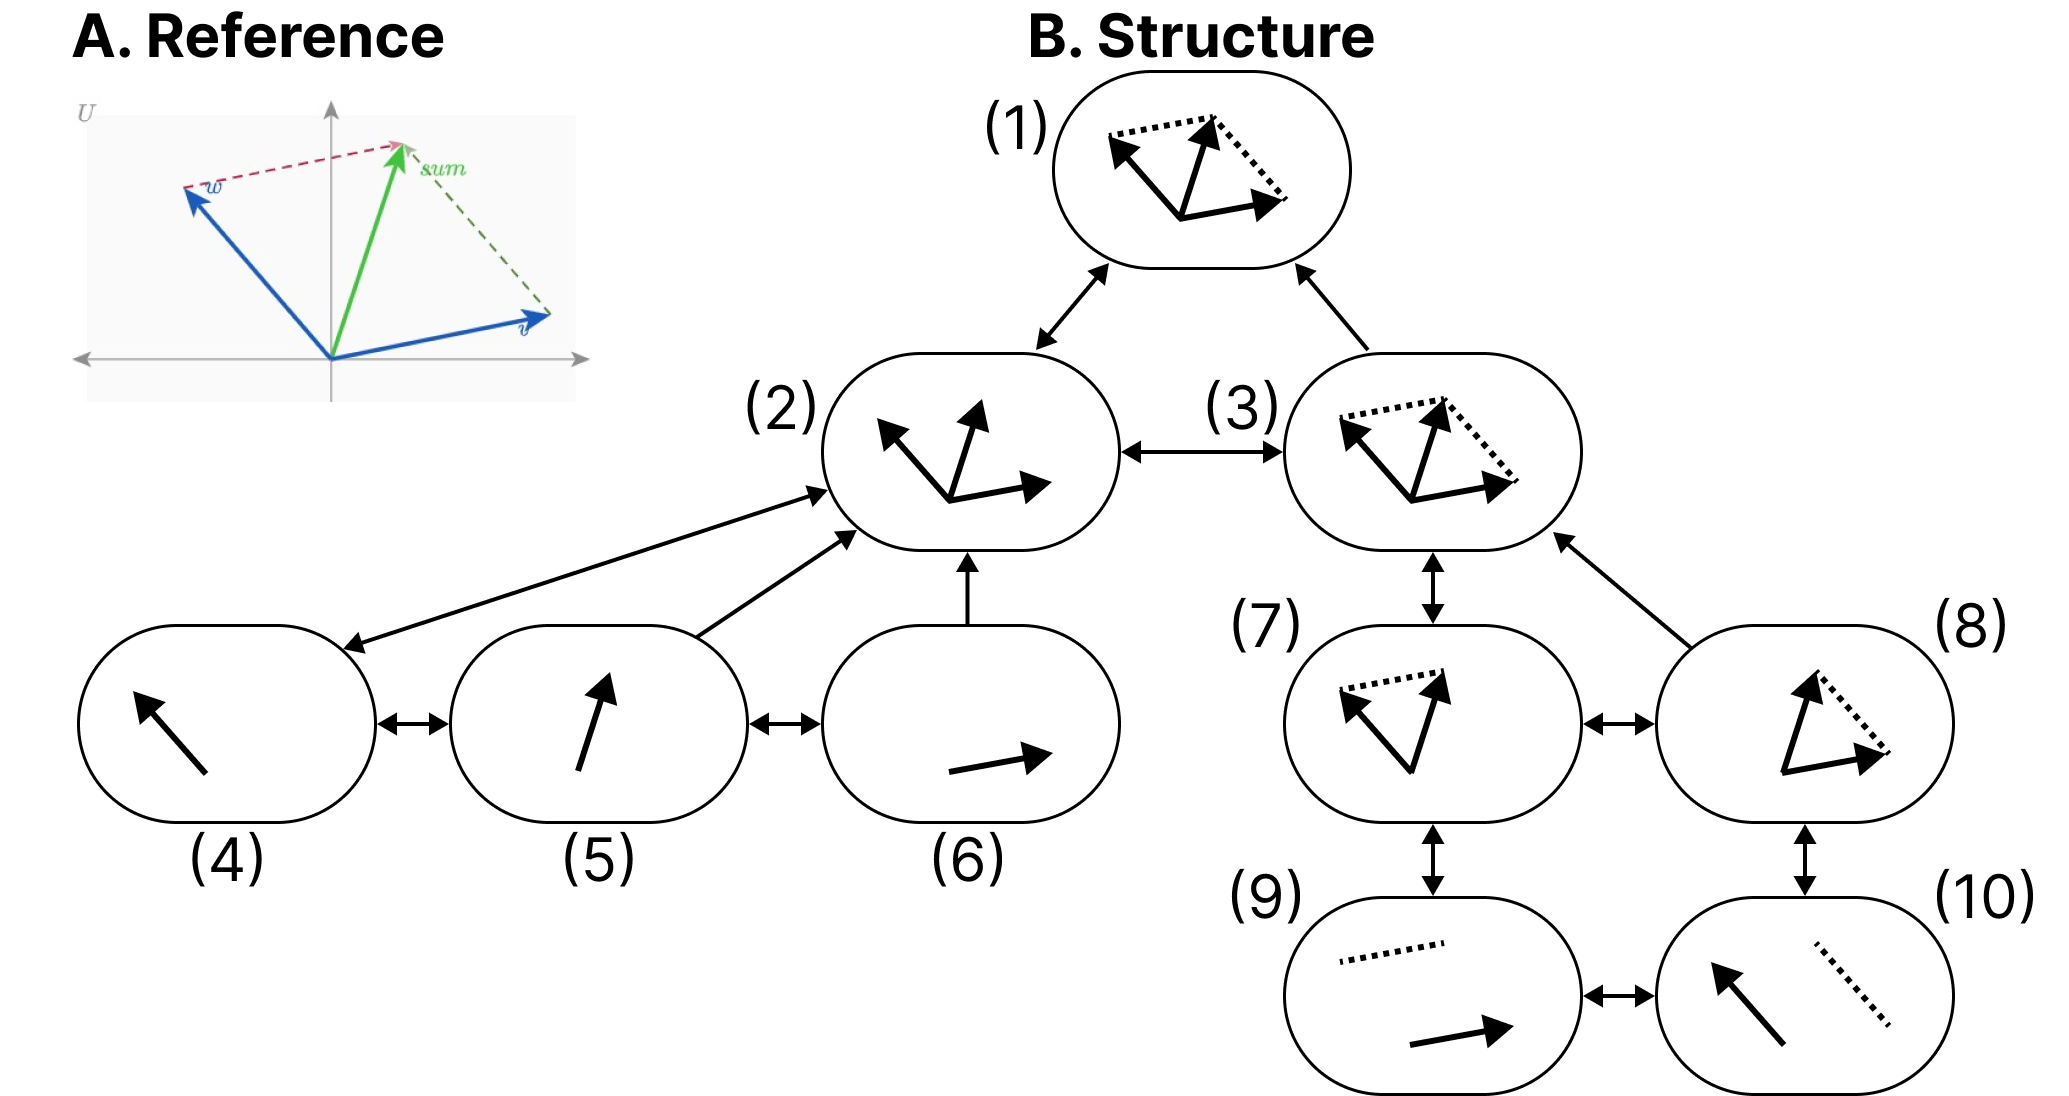
\includegraphics[width=0.75\linewidth]{figures/vectors.png}
  \caption{\textbf{A.} A reference image from \textit{Penrose} of a parallel vectors diagram. \textbf{B.} A diagram of our proposed structure, with two main sub-categories of information: understanding the vectors and their parallels.}
  % \Description{A mouse pointer is shown shaking over many data points that are very small while a touch hit area is shown over the same visualization, overlapping with many points at once.}
  \label{vectors}
\end{figure}

Our second prototype was a parallel vectors diagram (see~\Cref{vectors}). For the structure of this diagram we created a first level group that contains each vector and vector sum. The sibling to this grouping is another group which organizes sub-equations related to calculating each parallel vector. The sub equations each contain children that pair the sub equation with the vector it is parallel to.

Similar to \Cref{sets}, this figure maintains spatial relationships along the x dimension, does not have circular navigation, and allows drilling in and out.

% \textbf{Rendering.} The following descriptions correspond to the numbered nodes in \Cref{vectors}:
% \begin{enumerate}
%   \itemsep-0.4em
%   \item “Using the sum of Vectors A and B to form parallel vectors. Spatial view.”
%   \item “Vectors, group.”
%   \item “Sub-equations for parallel vectors, group.”
%   \item “Vector A [equation].”
%   \item “Sum of Vectors A and B.”
%   \item “Vector B [equation].”
%   \item “Connecting Vector A to the Sum Vector creates a parallel Vector to Vector B.”
%   \item “Connecting Vector B to the Sum Vector creates a parallel Vector to Vector A.”
%   \item “Parallel Vector A Sum AB and Vector B.”
%   \item “Parallel Vector B Sum AB and Vector A.”
% \end{enumerate}

\subsubsection{Discussion}
After our co-design sessions, our visual materials and navigation structures were used in the creation of functional prototypes. We additionally hand-crafted the descriptions and semantics for each node.

Accessibility work often takes a long time, from co-design to building to validation. But we believe that a well-articulated and useful design space, with tools that provide expressiveness and control over the dimensions of that design space, can improve how this work is done. The above case example demonstrates how builders who are thinking about data navigation design can rapidly scaffold prototypes for use in Data Navigator.

In particular, Data Navigator's design as a system gave our co-design sessions \textit{vocabulary correspondence}. Data Navigator's language helped us focus on the \textit{nodes, edges,} and \textit{navigation rules} for our \textit{structure} while we also explicitly discussed the \textit{rendering} details of \textit{coordinates, shapes, styling,} and \textit{semantics} for each node. The vocabulary of our design space directly corresponded with code details required to create a functional prototype.

% Our ability to develop these novel prototypes in a short turnaround time hinged on the design considerations of \textit{structure, navigation,} and \textit{description}~\cite{Zong2022Rich}. In addition, our deliverables are easy to integrate into a working, interactive prototype in Data Navigator because our system was designed to have \textit{vocabulary correspondence} these design dimensions. In an industry or research setting, these interactive prototypes could now be shared with other collaborators and stakeholders for further iteration.

We note that this co-design work is not intended to contribute a \textit{validated} set of designs. Rather, our contribution with this case example is to demonstrate that within the larger ecosystem of a research venture, Data Navigator is an improvement over designing and building navigable structures from scratch.

\section{Limitations and Future Work}
Data Navigator is a technical contribution, a system designed for appropriation~\cite{Dourish2003Appropriation} and adaptation~\cite{Wobbrock2011Ability} in different applied contexts. It is, as Louridas writes, a \textit{technical material}: a technology that enables new and useful capabilities~\cite{Louridas1999Bricolage}. While beyond the scope of the current paper, a critical next step for future work is to conduct separate studies with both practitioners and end users to evaluate Data Navigator's affordances.

Unlike toolkits that provide an end-to-end development pipeline for accessible visualization, Data Navigator serves as a low-level building block or material (like concrete). As such, one potential limitation of the framework is that it can be used to build both curbs (which are inaccessible) as well as ramps and \textit{curb-cuts} (which may be more broadly accessible).

Even when building more accessible curb-cuts, we stress the importance of actively involving people with disabilities in the design and validation of new ideas, in line with prior work~\cite{Reid2022Curb,Lundgard2019Sociotechnical,Lundgard2022Accessible,Zong2022Rich}. For example, while our first two case examples replicate co-designed and validated existing work, our third case example's co-designed prototypes would need to be validated with relevant stakeholders before wider implementation. Our system does not \textit{guarantee} any sort of accessibility on its own.

The diverse array of modalities supported by Data Navigator opens an immediate line of future work in engaging people with a correspondingly diverse set of disabilities. While recent explorations into accessible data visualization have been inspiring, this trend has primarily focused on the experiences of people with visual disabilities~\cite{Elavsky2022Chartability,Marriott,Kim2021Accessible}. More research should be conducted with other populations, particularly people who leverage assistive technologies beyond screen readers, to understand how interactive data visualizations can be better designed to serve them.

Finally, there are significant opportunities to improve the efficiency of our approach, including developing deterministic and non-deterministic methods to generate node-edge data and navigation rules from a visualization. Ma'ayan \ea stress in particular that reducing tedious complexity can contribute to the success of a well-designed toolkit~\cite{Maayan2020Domain}. Future work should identify areas where graphical interface tools or higher-level specifications can improve the experience of working with Data Navigator.

\section{Conclusion}
Practitioners at large continue to produce inaccessible interactive data visualizations, excluding people with disabilities. We believe that the burden of remediation first starts with the developers who build and maintain the toolkits that practitioners use.

However, the challenges faced by toolkit builders are significant. Most toolkits lack an underlying, navigable structure, support for broad input modalities used by people with disabilities, and meaningful, semantic rendering.

To engage these limitations we present Data Navigator, a technical contribution that builds on existing work towards a more generalizable accessibility-centered toolkit for creating data navigation interfaces. Data Navigator is designed for use by practitioners who both build and use existing toolkits and want a tool to make their data visualizations and interfaces more accessible.

We contribute a high-level system design for our node-edge graph-based approach that can be used to build data structures that are navigable by a wide array of assistive technologies and input modalities. Data Navigator is generic and can scaffold list, tree, graph, relational, spatial, diagrammatic, and geographic types of data structures common to data visualization.

Our system is designed to encourage both remediation of existing inaccessible systems and visualization formats as well as help scaffold the design of novel, future projects. We look forward to further research that explores the possibilities enabled by Data Navigator.

\chapter{\textit{Skeleton}: Visual Authoring of Non-visual Data Experiences}

\noindent\rule{16cm}{0.4pt}
\begin{quote}
This chapter was adapted from my paper, currently under review with IEEE VIS:
\begin{adjustwidth}{1cm}{}
% \-\hspace{2cm}
F. Elavsky, C. Nnadozie, L. Nadolskis, P. Carrington, and D. Moritz, ‘\textit{Skeleton}: Visual Authoring of Non-visual Data Experiences’, \textit{IEEE Transactions on Visualization and Computer Graphics}, 2026.
\end{adjustwidth}
\end{quote}
\noindent\rule{16cm}{0.4pt}

\begin{figure}[h]% specify a combination of t, b, p, or h for top, bottom, on its own page, or here
  \centering % avoid the use of \begin{center}...\end{center} and use \centering instead (more compact)
  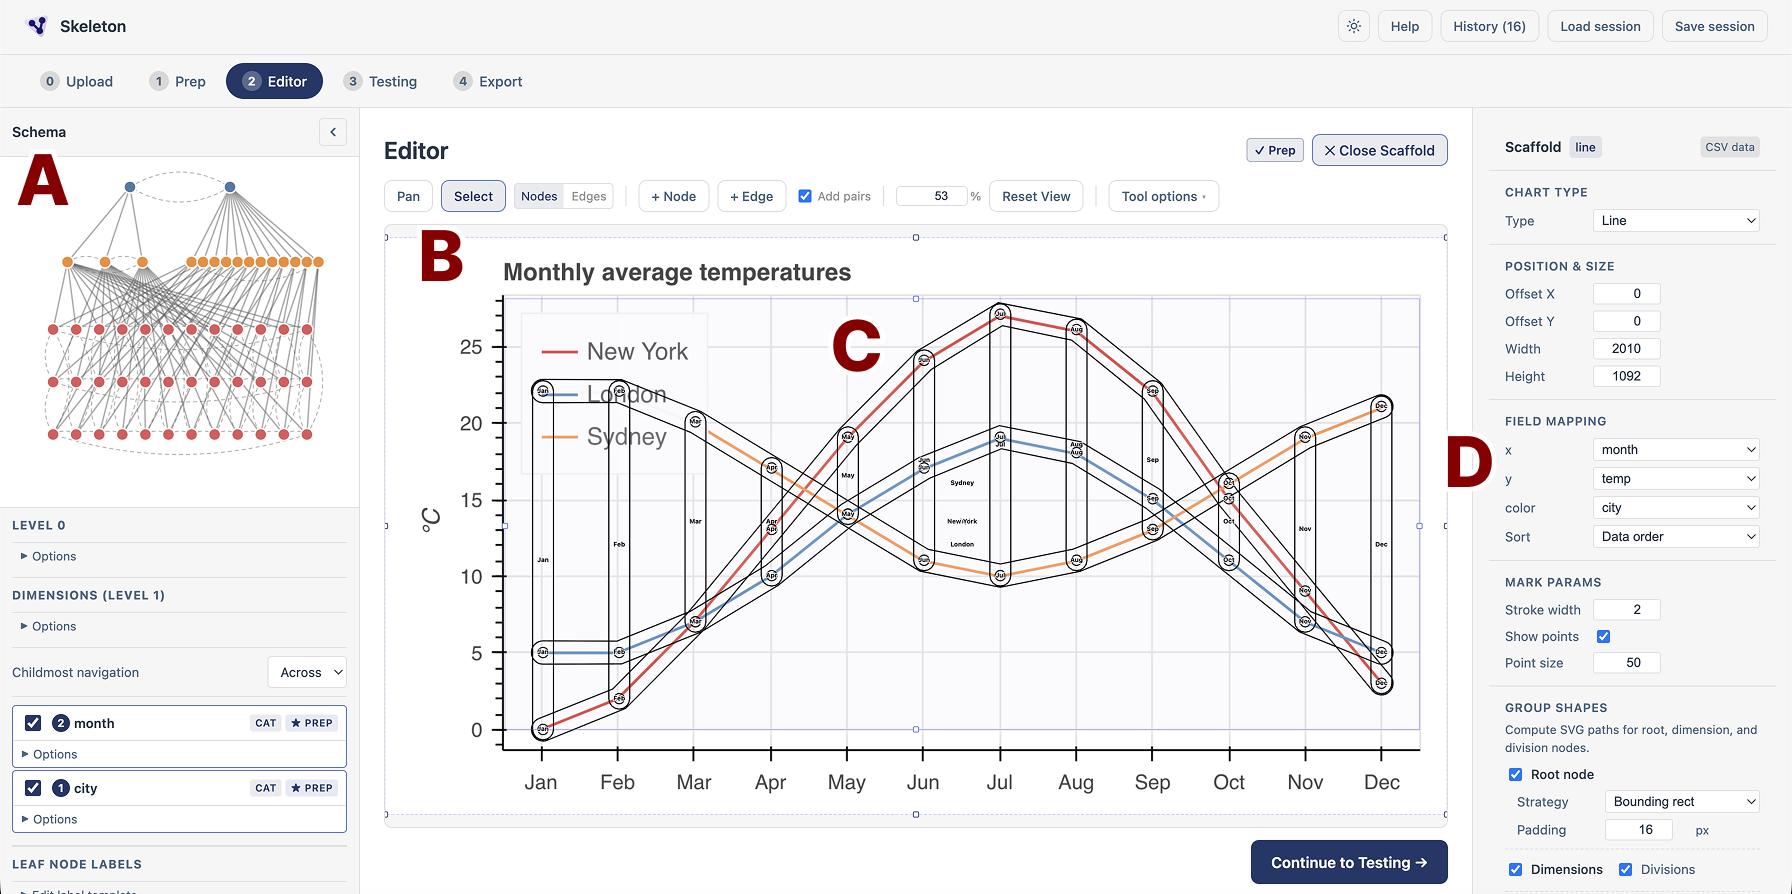
\includegraphics[width=15cm,height=15cm,keepaspectratio, alt={alt.}]{skeleton}
  \caption{%
  	Low-fidelity design draft of \textit{Skeleton}'s main user interface components and interactions. A. \textit{Skeleton}, our graphical user interface for creating and debugging screen reader navigation experiences of data visualizations. B. Users can add nodes wherever they want over the chart, manually or automatically with algorithmic assistance. C. Users can then ``draw'' edges between nodes, which signify navigation paths through the visualization.%
  }
  \label{fig:skeleton}
\end{figure}

\section{Abstract}
When sighted practitioners author accessible data visualizations, they build navigation structures (the nodes, edges, and input bindings that govern how assistive technologies traverse an interface) entirely in code, with no visual representation. This invisibility makes navigation structures difficult to inspect, debug, and iterate on. To sighted practitioners, every other aspect of a visualization is iterated on because it is visible; navigation structure ships as a first draft, if at all, because it is not. Without a representation to react to, practitioners cannot develop judgment about what makes navigation good or bad, and the quality ceiling of non-visual experiences is set by the absence of a feedback loop. We address this problem through longitudinal co-design with practitioners across cartography, design systems, and open-source visualization, and make three contributions. First, we introduce technical advancements for making the properties of accessible navigation structure visible and directly manipulable during authoring, grounded in two foundational pieces of infrastructure produced by our co-design work: an \textit{Inspector} that renders navigation graphs as interactive node-link diagrams, and a \textit{Dimensions API} that expresses navigation in terms of data dimensions rather than explicit graph construction. Second, building on these, we present \textit{Skeleton}, a direct-manipulation authoring environment in which the properties of an accessible navigation structure are translated into visual representations authors can observe and manipulate. Key techniques include a dual-view editor that simultaneously shows the system's navigation model and the end user's spatial experience, a scaffolding engine that automates spatial node placement by repurposing a visualization rendering pipeline, a live label-template editor with real-time screen-reader-output preview, and a testing mode that makes traversal sequence visually trackable. Third, we evaluate \textit{Skeleton} through an in-situ study with 8 practitioners across visualization design, engineering, and research. Making navigation structure visible changed how practitioners engaged with accessible design: they reconsidered the architecture of their own visualizations, attended to a broader range of input modalities, and shifted from treating accessibility as a compliance task to treating it as a design problem.

\section{Overview}

We start this work with a provocation: How might the discipline of visualization help the discipline of accessibility?

Visualization has spent decades developing techniques for a specific class of problem: representing and interacting with information visually. Grammars of visual encoding~\cite{Satyanarayan2017VegaLite,Wilkinson2011,McNutt2022,ZongAnimated2023,Wickham2010}, direct-interaction interfaces~\cite{Hutchins1985DirectManip,Endert2013,Shneiderman1992}, and iterative feedback loops between representation and understanding~\cite{Heer2007,Fisher2012,Liu2014} are all methods that enable abstraction and manipulation of the information that underlies the visual representation. We argue these methods have a direct application within the discipline's own accessibility challenges, one that has not yet been explored.

Sighted practitioners who build accessible data visualizations face an unusual authoring problem. The non-visual navigation structures they construct (the nodes, edges, focus states, input bindings, and semantics that govern how assistive technologies traverse a chart) exist only as code. A practitioner can write a navigation hierarchy, but cannot see it, click on a node to inspect what will be announced, observe the spatial relationship between a navigation path and the chart it overlays, and then manipulate its properties through direct interaction. Every other aspect of a visualization has a visible, inspectable representation during authoring: the visual encodings are visible, the layout is visible, the interaction states are visible. And yet, navigation structure is not.

This invisibility has practical consequences. Without a way to see what they are building, sighted practitioners cannot easily catch structural errors, compare design alternatives, and iterate. Accessibility becomes downstream of every other design choice, not because practitioners choose to deprioritize it, but because the authoring conditions do not support anything else~\cite{Joyner2022Wild, Sharif2024Challenges}. The floor and ceiling of non-visual data experiences are constrained by what sighted authors can perceive of their own work.

We engage this space with the following research questions:
\begin{enumerate}[label=\textbf{R\arabic*}, leftmargin=0pt, itemindent=!, itemsep=0pt, topsep=0.5em, parsep=0pt]
 
\item \label{rq:R1s}\textbf{(Qualitative, Exploratory):} What challenges do sighted practitioners face when designing and engineering navigation structures for accessible visualizations?
 
\item \label{rq:R2s}\textbf{(Qualitative, Exploratory):} How do sighted authors reason about the non-visual experiences that accompany their visualizations?
 
\item \label{rq:R3s}\textbf{(System, Design):} How can we make the properties of accessible navigation structure visible and directly manipulable during authoring?
 
\item \label{rq:R4s}\textbf{(Qualitative):} In what ways does a directly manipulable visual representation of navigation structure change how practitioners find errors and improve upon their designs?
 
\end{enumerate}
 
We address these questions through longitudinal co-design with practitioners across cartography, design systems, and open-source visualization, following an action research orientation~\cite{Hayes2011ActionResearch} in which the research team was embedded in each community's active development work. This paper makes three contributions:
 
First, \textbf{we introduce technical advancements} for making the properties of accessible navigation structure visible and directly manipulable during authoring. These techniques are grounded in our co-design collaborations, which produced two foundational pieces of infrastructure: an \textit{Inspector} that renders any navigation graph as an interactive node-link diagram, and a \textit{Dimensions API} that formalizes a declarative grammar for expressing navigation in terms of data dimensions rather than explicit graph construction~(\ref{rq:R1s}, \ref{rq:R2s}, \ref{rq:R3s}).
 
Second, building on this infrastructure, \textbf{we present \textit{Skeleton}, a direct-manipulation authoring environment} in which the topology, spatial mapping, semantics, and input logic of an accessible navigation structure are made visible and directly manipulable. \textit{Skeleton} is built on Data Navigator~\cite{Elavsky2023}, a code-based library for constructing interactive data navigation structures~(\ref{rq:R3s}). Our intention with \textit{Skeleton} is to continue to develop it towards a usable, practical system beyond the scope of this research.
 
Third, \textbf{we contribute findings from an in-situ interview study} with 8 practitioners across visualization design, engineering, and research. We evaluate Skeleton as a design probe~\cite{Hammad2024GameAware,Hutchinson2003TechnologyProbes} rather than a deployable system, focusing on qualitative shifts in practitioner engagement rather than task performance. We find that making navigation structure visible shifted how participants engaged with accessible design: they reconsidered the architecture of their own visualizations, attended to a broader range of input modalities, and shifted from treating accessibility as a compliance task to treating it as a design problem~(\ref{rq:R1s}, \ref{rq:R2s}, \ref{rq:R4s}).

% This paper makes three contributions towards these challenges:

% First, this work \textbf{introduces techniques for making the properties of accessible navigation structure visible and directly manipulable during authoring}. We develop these techniques through longitudinal co-design with practitioners across cartography, design systems, and open-source visualization, following an action research orientation~\cite{Hayes2011ActionResearch} in which the research team was embedded in each community's active development work. These collaborations established both the need for visual representations of navigation structure and produced foundational infrastructure: an \textit{Inspector} for rendering navigation graphs as interactive diagrams, and a \textit{Dimensions API} that formalizes a declarative grammar for expressing navigation in terms of data dimensions.

% Building on this infrastructure, \textbf{we present \textit{Skeleton}, a direct-manipulation authoring environment} in which the topology, spatial mapping, semantics, and input logic of an accessible navigation structure are made visible and directly manipulable. \textit{Skeleton} is built on \textit{Data Navigator}~\cite{Elavsky2023}, a code-based library for constructing interactive data navigation structures.

% Lastly, to evaluate how making navigation structure visible changes practitioner engagement with accessible design, \textbf{we contribute our findings from an in-situ interview study} with 8 practitioners across visualization design, engineering, and research.

% Across our contributions in this paper, we investigate the following research questions:
% \begin{enumerate}[label=\textbf{R\arabic*}, leftmargin=0pt, itemindent=!, itemsep=0pt, topsep=0.5em, parsep=0pt]

% \item \label{rq:R1}\textbf{(Qualitative, Exploratory):} What challenges do sighted practitioners face when designing and engineering navigation structures for accessible visualizations?

% \item \label{rq:R2}\textbf{(Qualitative, Exploratory):} How do sighted authors reason about the non-visual experiences that accompany their data visualizations?

% \item \label{rq:R3}\textbf{(System, Design):} How can we make the properties of accessible navigation structure visible and directly manipulable during authoring?

% \item \label{rq:R4}\textbf{(Qualitative):} In what ways does a directly manipulable visual representation of navigation structure change how practitioners find errors and improve upon their designs?

% \end{enumerate}

% We find that making navigation structures visible shifted how participants engaged: they reconsidered the architecture of their own visualizations, attended to a broader range of input modalities, and developed substantive interest in what constitutes ``good'' non-visual data navigation and interaction.

\section{Related Work}

\subsection{Non-visual Data Experiences}

Blind people who rely on assistive technologies interact with data in fundamentally different ways than sighted users who use a direct pointer, like a mouse~\cite{Marriott, Kim2021Accessible, Sharif2021}. A substantial body of research has documented what these experiences look like across modalities, and what it takes to make them meaningful. In the context of ``data experiences,'' this paper focuses specifically on interactive navigation structures, but we briefly survey adjacent modalities to situate our contribution.

\textbf{Alternative text and natural language.} A dominant strand of this work concerns the generation and evaluation of textual descriptions of visualizations~\cite{Lundgard2022Accessible, Jung2022Communicating, Kim2023Beyond, Kim2023Explain}. More recent LLM-driven systems and Q/A approaches can caption charts with varying degrees of semantic depth, some at a risk of producing bias~\cite{Farahani2023, Elavsky2025, Kim2023Exploring}. While alt text makes a visualization's message available without sight, it is by nature static: a description conveys what a visualization says, but not how a user might explore or interact with it.

\textbf{Sonification, haptics, and tactile rendering.} Non-visual data experiences extend well beyond text. Sonification encodes data as sound~\cite{Hermann2011, Mansur1985Sound, Brewster2002Visualization}, with declarative grammars emerging for authoring these experiences~\cite{Kim2024}. Haptic and tactile representations offer another channel through refreshable displays, 3D-printed graphics, and multimodal touchscreen interactions~\cite{Butler2021Technology, Marriott2026, Holloway2024, Reinders2025}. Recent systems integrate multiple non-visual modalities around a single data representation~\cite{Seo2024, Holloway2022, Chundury2022Towards}.

% For other modalities, such as tactiles and sonifications, there are readily-available visual translations and adjacent or co-equal representations~\cite{Zong2024, Wimer2026}. A tactile graphic can be touched and seen. A sonification can be heard and visualized. Interactive navigation structures, by contrast, are experienced interactively through sound by end users yet have no visible representation; they are not multi-modal.

\textbf{Interactive navigation structures.} The primary focus of our work centers on the state of research related to structured navigation: the traversal of data points, groupings, and interface elements through assistive technologies and keyboard input~\cite{Sorge2016Polyfilling, WAI2017Keyboard, Zong2022Rich, Elavsky2023}. Existing systems and interfaces have demonstrated that going beyond static descriptions to support hierarchical, traversable data structures meaningfully improves how blind users can explore and reason about charts~\cite{Zong2022Rich, Thompson2023Chart}. Giving users control over the textual tokens surfaced during navigation improves comprehension and agency~\cite{Jones2024}. And more recent work has found that perceptually congruent navigation structures for charts and diagrams can improve goal-driven exploration~\cite{Mei2025}.

% , and Umwelt~\cite{Zong2024} introduces a structured editing environment for authoring multi-modal representations including navigation. Data Navigator~\cite{Elavsky2023} similarly provides a toolkit for constructing arbitrary navigation graphs over data, enabling traversal patterns that more constrained libraries or architectures cannot express.

% This is the gap our work addresses.

% They exist as code, are experienced through interaction and sound by end users, but offer sighted practitioners nothing to see, inspect, or manipulate. 

\subsection{Authoring Non-visual Data Experiences}

Accessible visualization has historically centered the experiences of disabled users, but a parallel and increasingly urgent body of work examines the experiences of the people who build these experiences: visualization designers, engineers, and researchers.

\textbf{Practitioner challenges.} Research consistently finds that sighted visualization practitioners struggle with accessibility~\cite{Joyner2022Wild, Fan2023Accessibility, Sharif2024Challenges}. Most visualizations in the wild are inaccessible and designers themselves report lacking guidance, especially for complex and interactive graphics~\cite{Joyner2022Wild,Sharif2024Challenges}. And screen reader users experience the downstream effects of these gaps: inconsistent structure, poor keyboard support, and information that is present visually but absent in the accessibility tree~\cite{Sharif2021, Fan2023Accessibility}. The pattern across this work is consistent: the practitioners who build visualizations lack the tools and feedback mechanisms to make non-visual experiences effective, useful, and good.

Across practitioner-centered literature, a recurring finding is that non-visual experiences are treated as downstream of visual design choices, added after the visual representation is finished rather than designed in parallel~\cite{Joyner2022Wild, Lundgard2019Sociotechnical, Sharif2024Challenges, Zong2024}. This sequencing has consequences: what is navigable and how it is structured is constrained by whatever visual decisions came first.

% \textbf{Evaluation tooling.} One response to practitioner challenges has been the development of evaluation frameworks. Chartability~\cite{Elavsky2022Chartability} provides a heuristic-based auditing methodology that translates WCAG and domain-specific criteria into actionable checks for visualization practitioners. While Chartability helps practitioners identify failures, it does not help them design or author non-visual experiences from the ground up.

\textbf{Authoring-oriented systems.} A distinct line of work has focused on building authoring tools and libraries that give practitioners more tractable paths to accessible output. Few visualization tools support the kinds of interactive navigation structures that assistive technology users most benefit from~\cite{Kim2023Beyond}. Of those that do, most rely on code-based approaches~\cite{Blanco2022olli,Sharif2018evoGraphs,Sharif2022VoxLens,Elavsky2023}. \textit{Umwelt}~\cite{Zong2024} takes a different and notable approach: it is a structured editing environment where authors specify representations \textit{across} modalities (sonification and visualization) in an integrated interface, where navigation is made available over the visualization using \textit{Olli}~\cite{Blanco2022olli}. The latest work in this space is \textit{Arboretum}, a tool that provides automatic conversion of diagrams to a tabular structure, navigable structure, and tactile representation~\cite{Wimer2026}. In \textit{Arboretum}, the input visual is treated as the ground truth for the navigation structure, which is treated as downstream output.

\textbf{Communicating visually, authoring invisibly.} There is a revealing irony across this body of related work: research about navigation structures almost invariably communicates those structures visually. Papers such as ``rich screen reader experiences''~\cite{Zong2022Rich}, \textit{ChartReader}~\cite{Thompson2023Chart}, \textit{Benthic}~\cite{Mei2025}, and \textit{Data Navigator}~\cite{Elavsky2023} each use visual node-link diagrams and hierarchical schematics to explain navigation paths to their readers. The same pattern holds in adjacent domains that involve structuring data for navigation, such as PDF remediation~\cite{Mowar2026iTagPDF}.

And in authoring-oriented systems, none provide a visual interface through which practitioners can interactively inspect and manipulate navigation structures as a first-class design material. Structure output is either downstream of code or static visuals. Structure is always \textit{derived} or \textit{specified}; indirectly manipulated. Additionally, verification of the structure across all of these systems requires developers to manually navigate using a screen reader after the structure has been authored and rendered, before returning to the upstream visual design space or code.

Navigation structure is understood and communicated visually by sighted researchers and designers, yet built entirely without visual feedback by developers. We seek to address this gap.

% The key characteristic that distinguishes interactive navigation from alt text, tactile, and sonic representations is that navigation structures have no visible representation \textit{during} authoring.

% There is no visual feedback loop, no way to see the structure as a whole and manipulate it directly. This is the problem we address.

% We conjecture that making non-visual structures visible is a precondition for sighted authors treating it as a genuine design material, because visual representations serve as locations for communication, reflection, and iteration.

% when navigation structure is not visible to the people building it, it cannot be iterated on.

% \subsection{Direct Manipulation and Visualization}

% We intended to build \textit{Skeleton} as a direct manipulation system: practitioners observe and modify navigation structures through interactive graphical representations rather than code alone. Direct manipulation interfaces provide a continuous representation of objects of interest, support physical actions on those objects, and give rapid, incremental feedback~\cite{Shneiderman1983DirectManip, Hutchins1985DirectManip}. These properties have been foundational to visualization systems from dynamic queries~\cite{Shneiderman1992} to visual analytics~\cite{Endert2013}. When an artifact is visible and manipulable, designers iterate more, catch more problems, and explore alternatives they would not consider in a code-only medium~\cite{Schon1996Relective, Maayan2020Domain}.

% Rendering navigation structures graphically makes them available as design materials in the same way.

% Grammars of interactive graphics such as Vega-Lite~\cite{Satyanarayan2017VegaLite} express visual encoding at the level of data fields rather than explicit mark construction, making visualization structure writable at a higher level of abstraction~\cite{Bostock2011D3}. The \textit{Dimensions API} applies the same principle to navigation: it lets practitioners describe traversal in terms of data dimensions rather than hand-wired graph construction, at an abstraction level that corresponds to how they already think about their data.


%

\section{Co-design Foundations}
\label{sec:codesign}

% The problem this paper addresses emerged from practice: from longitudinal collaborations with practitioners actively building accessible data experiences, who kept encountering the same friction from different directions.  I, the primary author, was a co-designer and co-engineer on these teams and their projects, which in turn informed the work that led to \textit{Skeleton}'s development. 

Our research follows an \textit{action research} orientation~\cite{Hayes2011ActionResearch}, in which knowledge is generated by engaging with a community to solve a real problem in-situ, alongside them rather than studying it from the outside. These collaborations started from a shared motivation: practitioners needed to make their existing systems accessible to navigational assistive technologies, using Data Navigator~\cite{Elavsky2023} as a foundation. Across three projects, we worked with 12 individuals outside our research team. Three blind co-designers shaped the work throughout: CD1 and CD2 (anonymous) and a co-author on this paper, [REDACTED]. CD1's contributions are noted in \Cref{sec:geomap}, CD2's are noted in \Cref{sec:testing}. [REDACTED] contributed to early ideation, problem formation, and framing for the project as a whole, helping define the authoring challenges that \textit{Skeleton} addresses, in addition to feedback on study design.

The co-design literature on accessibility has centered people with disabilities as primary design partners~\cite{Cullen2019Co, Race2023, deGreef2021Interdependent, Thompson2023Chart, Zong2022Rich, Zong2025}, and rightly so. Our co-design takes sighted practitioners as primary partners because the authoring challenges we address happen on the sighted side of the process: it is sighted authors who cannot see what they are building.

Two themes converged across all three engagements, and we present them here before describing the individual projects that surfaced them. First, \textbf{practitioners communicated and reasoned about accessible navigation using visual representations}: while designing for language, sound, and structure, our collaborators drew on paper, built wireframes of nodes and edges, and reflected on the design space using visual artifacts. Even when collaborating with blind co-designers, a visual medium was the first language of sighted authors. Second, \textbf{development that followed visual design work faced severe iteration barriers}: verifying a navigation experience required building a working code prototype and manually navigating it with a screen reader. The gap between visual design and code-based scaffolding with manual testing produced repeated mistakes, misinterpretations, and abandoned prototypes. Each project below contributed distinct evidence for these themes and surfaced specific requirements that shaped our infrastructure and tooling.

\subsection{Geologic Map}
\label{sec:geomap}

\begin{figure}[h]% specify a combination of t, b, p, or h for top, bottom, on its own page, or here
  \centering % avoid the use of \begin{center}...\end{center} and use \centering instead (more compact)
  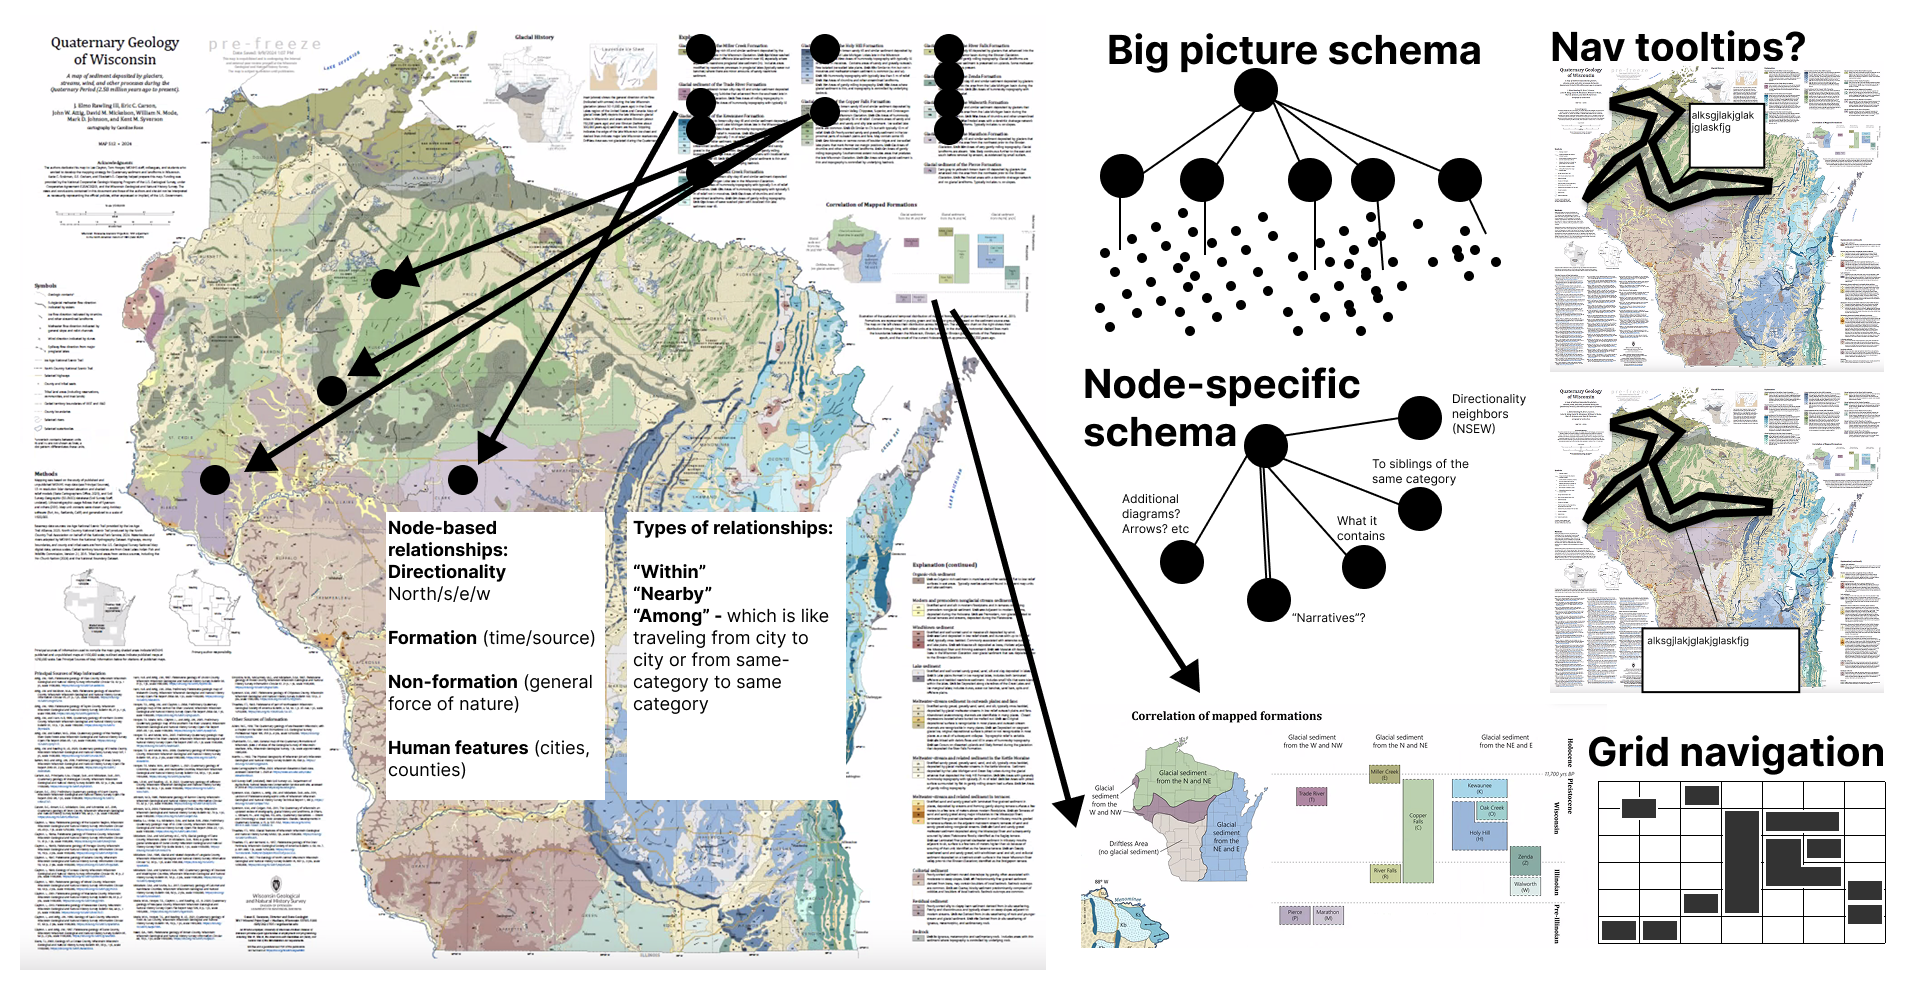
\includegraphics[width=\columnwidth, alt={A zoomed out view of the state of Wisconsin, encoded with a tapestry of dozens of colors and textures. Arrows annotate direction from the legend to map area, a separate area has messy, approximated graph structures laid out, a zoomed in version of a chart inside the graphic has schematics next to it titled "grid navigation." An area in the upper corner demonstrates 2 different styles of drawing tooltips during navigation.}]{figures/geologic.png}
  \caption{%
  	Our visual design work in Figma over a static geologic infographic map of Wisconsin. We use visual forms and illustrations over and beside the map to communicate flows, structure, navigation styles, and interaction patterns.%
  }
  \label{fig:geo}
\end{figure}

Our longest engagement spanned just over two years, with a cartographer, accessibility consultant, and blind co-designer (CD1) building an interactive version of a quaternary geologic map of Wisconsin~\cite{Rawling2025}. The map combined dozens of irregular geographic regions organized categorically by a legend.

Early design sessions took place in Figma (\Cref{fig:geo}), where we laid out node-link diagrams of how a screen reader user might traverse the map, legend, and peripheral information. We annotated each node with text a screen reader would announce and connected them to relevant regions. Drawing the structure made it possible to discuss design choices, catch dead ends, and debate traversal strategies. We were informally doing what \textit{Skeleton} later formalized.

The friction began when we moved from design to implementation. We had no way to verify that our designed structure would be good or ideal, and scaffolding the project into Data Navigator was arduous: the translation from even simple navigational designs to functional code was too complex to hand off or meaningfully iterate on. The collaboration also surfaced a design-space boundary: for within-map spatial navigation, an egocentric audio-game approach~\cite{Biggs2022Audiom} fit better than a node-link graph, a distinction CD1 helped surface. Reaching this boundary was only possible because we could see the structure we were trying to build.

\subsection{Design System Library}
\label{sec:designsystem}

Our second engagement, spanning 7 months, was with 6 engineers and designers on Adobe's React Spectrum Charts library, an open-source chart component system. We worked in their codebase and in Miro on navigation design for bar charts, clustered and stacked bars, line charts, and related types. Because we needed generalized, reusable patterns, our design problems differed from the geologic map: we needed to account for use, re-use, and edge cases across chart types.

Our Miro sessions produced two kinds of artifacts: diagrams of navigation structure for specific chart \textit{instances} and \textit{schema} diagrams capturing generalized patterns in dimensional terms. The concept of a ``dimension'' emerged naturally: common transformations on Data Navigator's graph structure corresponded to properties within a dataset, such as a ``categorical'' dimension or a ``numerical'' dimension, where traversal took place within collections of grouped siblings. This dimensional thinking directly foreshadowed the Dimensions API (\Cref{sec:infrastructure}).

The dominant friction was iteration speed. We could sketch and converge on a schema in Miro in an hour, but verifying the design in a functional example required embedding Data Navigator into a large codebase, implementing changes, rebuilding, and manually testing with a screen reader. The collaboration also surfaced a limitation: mobile screen reader navigation uses swipe gestures rather than keyboard input, and our keyboard interaction model did not account for it. Together, these gaps made two requirements clear: a higher-level navigation abstraction and a visual tool for inspecting structures without a screen reader or a fully integrated build.

\subsection{Open Source Visualization Library}
\label{sec:opensource}

Our third collaboration, spanning nearly two years, was with Quansight Labs and contributors to Bokeh, a Python-based open-source visualization library. We performed an accessibility audit~\cite{Eswaramoorthy2025BokehAudit} based on Chartability~\cite{Elavsky2022Chartability} and identified that Bokeh visualizations with interactive chart elements needed to be navigable by assistive technologies.

Unlike Adobe, Bokeh has no native chart types. Its API operates at the level of glyphs, renderers, and data sources, which users assemble freely. There was no standard unit around which to anchor a navigation pattern, and any grammar or tooling would need to accommodate an open-ended range of encoding combinations. The iteration gap from Adobe was present in a more severe form: making library-wide contributions to a fully open-source project required incremental tooling for the most common cases. For Bokeh, we needed to test functional, data-driven navigation abstractions without fully embedding Data Navigator into the library.

%%

\subsection{Infrastructure from Practice}
\label{sec:infrastructure}

%
The three collaborations converged on two concrete requirements: a way to visually render and inspect navigation structures, and a higher-level abstraction for specifying navigation without hand-wiring every node and edge. We built two pieces of infrastructure to address these requirements. Both were used in subsequent co-design work and became the foundation on which \textit{Skeleton} was built.

\subsubsection{An Inspector Gadget}

We built an \textit{Inspector} (\texttt{@data-navigator/inspector}) to render any Data Navigator structure as an interactive node-link graph using D3, with an accompanying console for debugging. Hierarchical structures are colored by level; edges are drawn as directed links; the entry point is visually marked. The \textit{Inspector}'s graph can itself be navigated using Data Navigator, with visual focus tracking during navigation, allowing practitioners to manually verify structure and reachability.

This made structural verification immediate: a practitioner could generate a structure and check at a glance whether the hierarchy had the right levels, whether circular extents produced expected wrap-around edges, or whether a particular path was reachable. The interactive console logs API information and underlying data when nodes are activated, and hovering or focusing logged information highlights the corresponding node in the graph.

The \textit{Inspector} remains a developer tool, however. It requires code familiarity to attach and renders structure as an abstract graph with no connection to the spatial layout of the underlying visualization. It shows topology but not instantiated geometry: a practitioner can see that two nodes are connected but not where their focus indicators will appear on-screen. This gap between navigable structure and its spatial instantiation over a rendered chart motivated \textit{Skeleton}.

\subsubsection{Alternative Dimensions}

The original Data Navigator library requires explicit graph construction: practitioners specify nodes, edges, and navigation rules by hand. This is general but scales poorly.

The \textit{Dimensions API} introduces a declarative abstraction one level above this. Rather than specifying the graph directly, a practitioner describes the \textit{dimensions} of their data, the meaningful axes along which a user might want to navigate, and the API constructs the full node-link structure automatically. A dimension has a type (\texttt{categorical} or \texttt{numerical}), a data key, and behavioral properties governing traversal. Two properties are central: \texttt{extents} determines boundary behavior (\texttt{terminal} stops at edges; \texttt{circular} wraps around), and \texttt{childmostNavigation} determines whether leaf-level nodes are reachable laterally across a dimension's divisions without first returning to a parent.

The generated structure is a multi-level hierarchy: each dimension produces a root node, below which division nodes group the data, below which leaf nodes represent individual data points. Multiple dimensions over the same dataset share leaf nodes, so users navigating via different dimensions reach the same data through different paths. With the Dimensions API, bar chart navigation that would otherwise require constructing every node and edge by hand is expressed as a single dimension declaration:

\begin{verbatim}
dimensions: {
  values: [
    { 
      dimensionKey: 'month',
      type: 'categorical',
      behavior: { extents: 'circular' }
    }
  ]
}
\end{verbatim}

The abstraction is chart-type-agnostic: bar charts, scatter plots, line charts, and layered charts all use the same vocabulary, with different combinations producing different navigation topologies. This directly addressed Bokeh's problem: the API mirrors data fields and encoding choices as a set of dimensions.


\section{\textit{Skeleton}: System Design}
\label{sec:skeleton}


With a visual structure renderer (the Inspector) and a declarative abstraction for producing navigation structures (the Dimensions API), the remaining problem was to bring these capabilities into an integrated, direct-manipulation authoring environment where practitioners could not only see structure but manipulate it interactively, test it with real input, and iterate on it with immediate feedback. \textit{Skeleton} is that environment. It integrates the Inspector and Dimensions API into a unified workflow and extends both with a guided preparation phase, a spatial rendering canvas, and a live testing mode. Each of Skeleton's authoring techniques makes visible a specific property of non-visual interaction that sighted practitioners otherwise cannot see during authoring: the topology of what is navigable, the spatial mapping of where navigation lives over the chart, the semantics of what is announced, and the temporal sequence in which a user encounters nodes.

Where the Inspector requires a practitioner to write code first and visualize after, \textit{Skeleton} reverses the direction: practitioners design a navigation structure visually and inspect the code representation as a consequence of that design.

\subsection{Staging: Input and Preparation for Authoring}

The authoring workflow proceeds through four stages: upload, prepare, edit, and test. Making a visualization accessible involves decisions about what is navigable, how navigation is triggered, and where focus indicators appear in space. These decisions are related but distinct, and collapsing them into a single undifferentiated interface, as code-only workflows effectively do, makes each one harder to reason about. The stage architecture surfaces them as separate concerns. It also preserves a direct correspondence between what practitioners see in the interface and the structure of the Data Navigator API~\cite{Elavsky2023}: each stage maps onto a distinct layer of the API, lowering the barrier to moving from visual authoring into code when production deployment requires it.

\textbf{Upload.} The upload phase is deliberately permissive. Practitioners can bring a dataset, a chart image, both, or neither. When a dataset is present, \textit{Skeleton} parses its fields and infers dimension types automatically, producing a default, starting configuration for the \textit{Prepare} step. When only an image is present, practitioners proceed directly to editing and construct nodes and edges manually over the image. This was motivated by our geologic map co-design work: many bespoke visualizations do not have a single underlying dataset, and any tool that requires structured data as a precondition for excludes the cases that need it most. \textit{Skeleton} can be applied to any 2D image surface, not only to visualizations in the conventional sense.

\textbf{Prepare.} The prepare stage addresses a hard authoring bottleneck: not placing nodes, but deciding what structure to build at all. A practitioner who has never designed a navigation structure faces an open configuration space with no obvious entry point. The prep stage presents a four-chapter Q\&A wizard that moves through authoring decisions sequentially: (1) whether the chart should have a root node and what it should announce, (2) which data fields should be navigable dimensions and how those dimensions should behave at their boundaries, (3) which keyboard interactions each dimension should be assigned to, and (4) what text labels each level of the hierarchy should produce. Each chapter is accompanied by an illustrative schematic diagram of which part of the heirarchy is being edited as well as a diagram showing examples of what these decisions look like when showing on a chart. The wizard's output populates a configuration in the editor that practitioners can then inspect, refine, and revise.

\subsection{Edit: Interacting with Topology, Layout, and Semantics}

\begin{figure}[h]% specify a combination of t, b, p, or h for top, bottom, on its own page, or here
  \centering % avoid the use of \begin{center}...\end{center} and use \centering instead (more compact)
  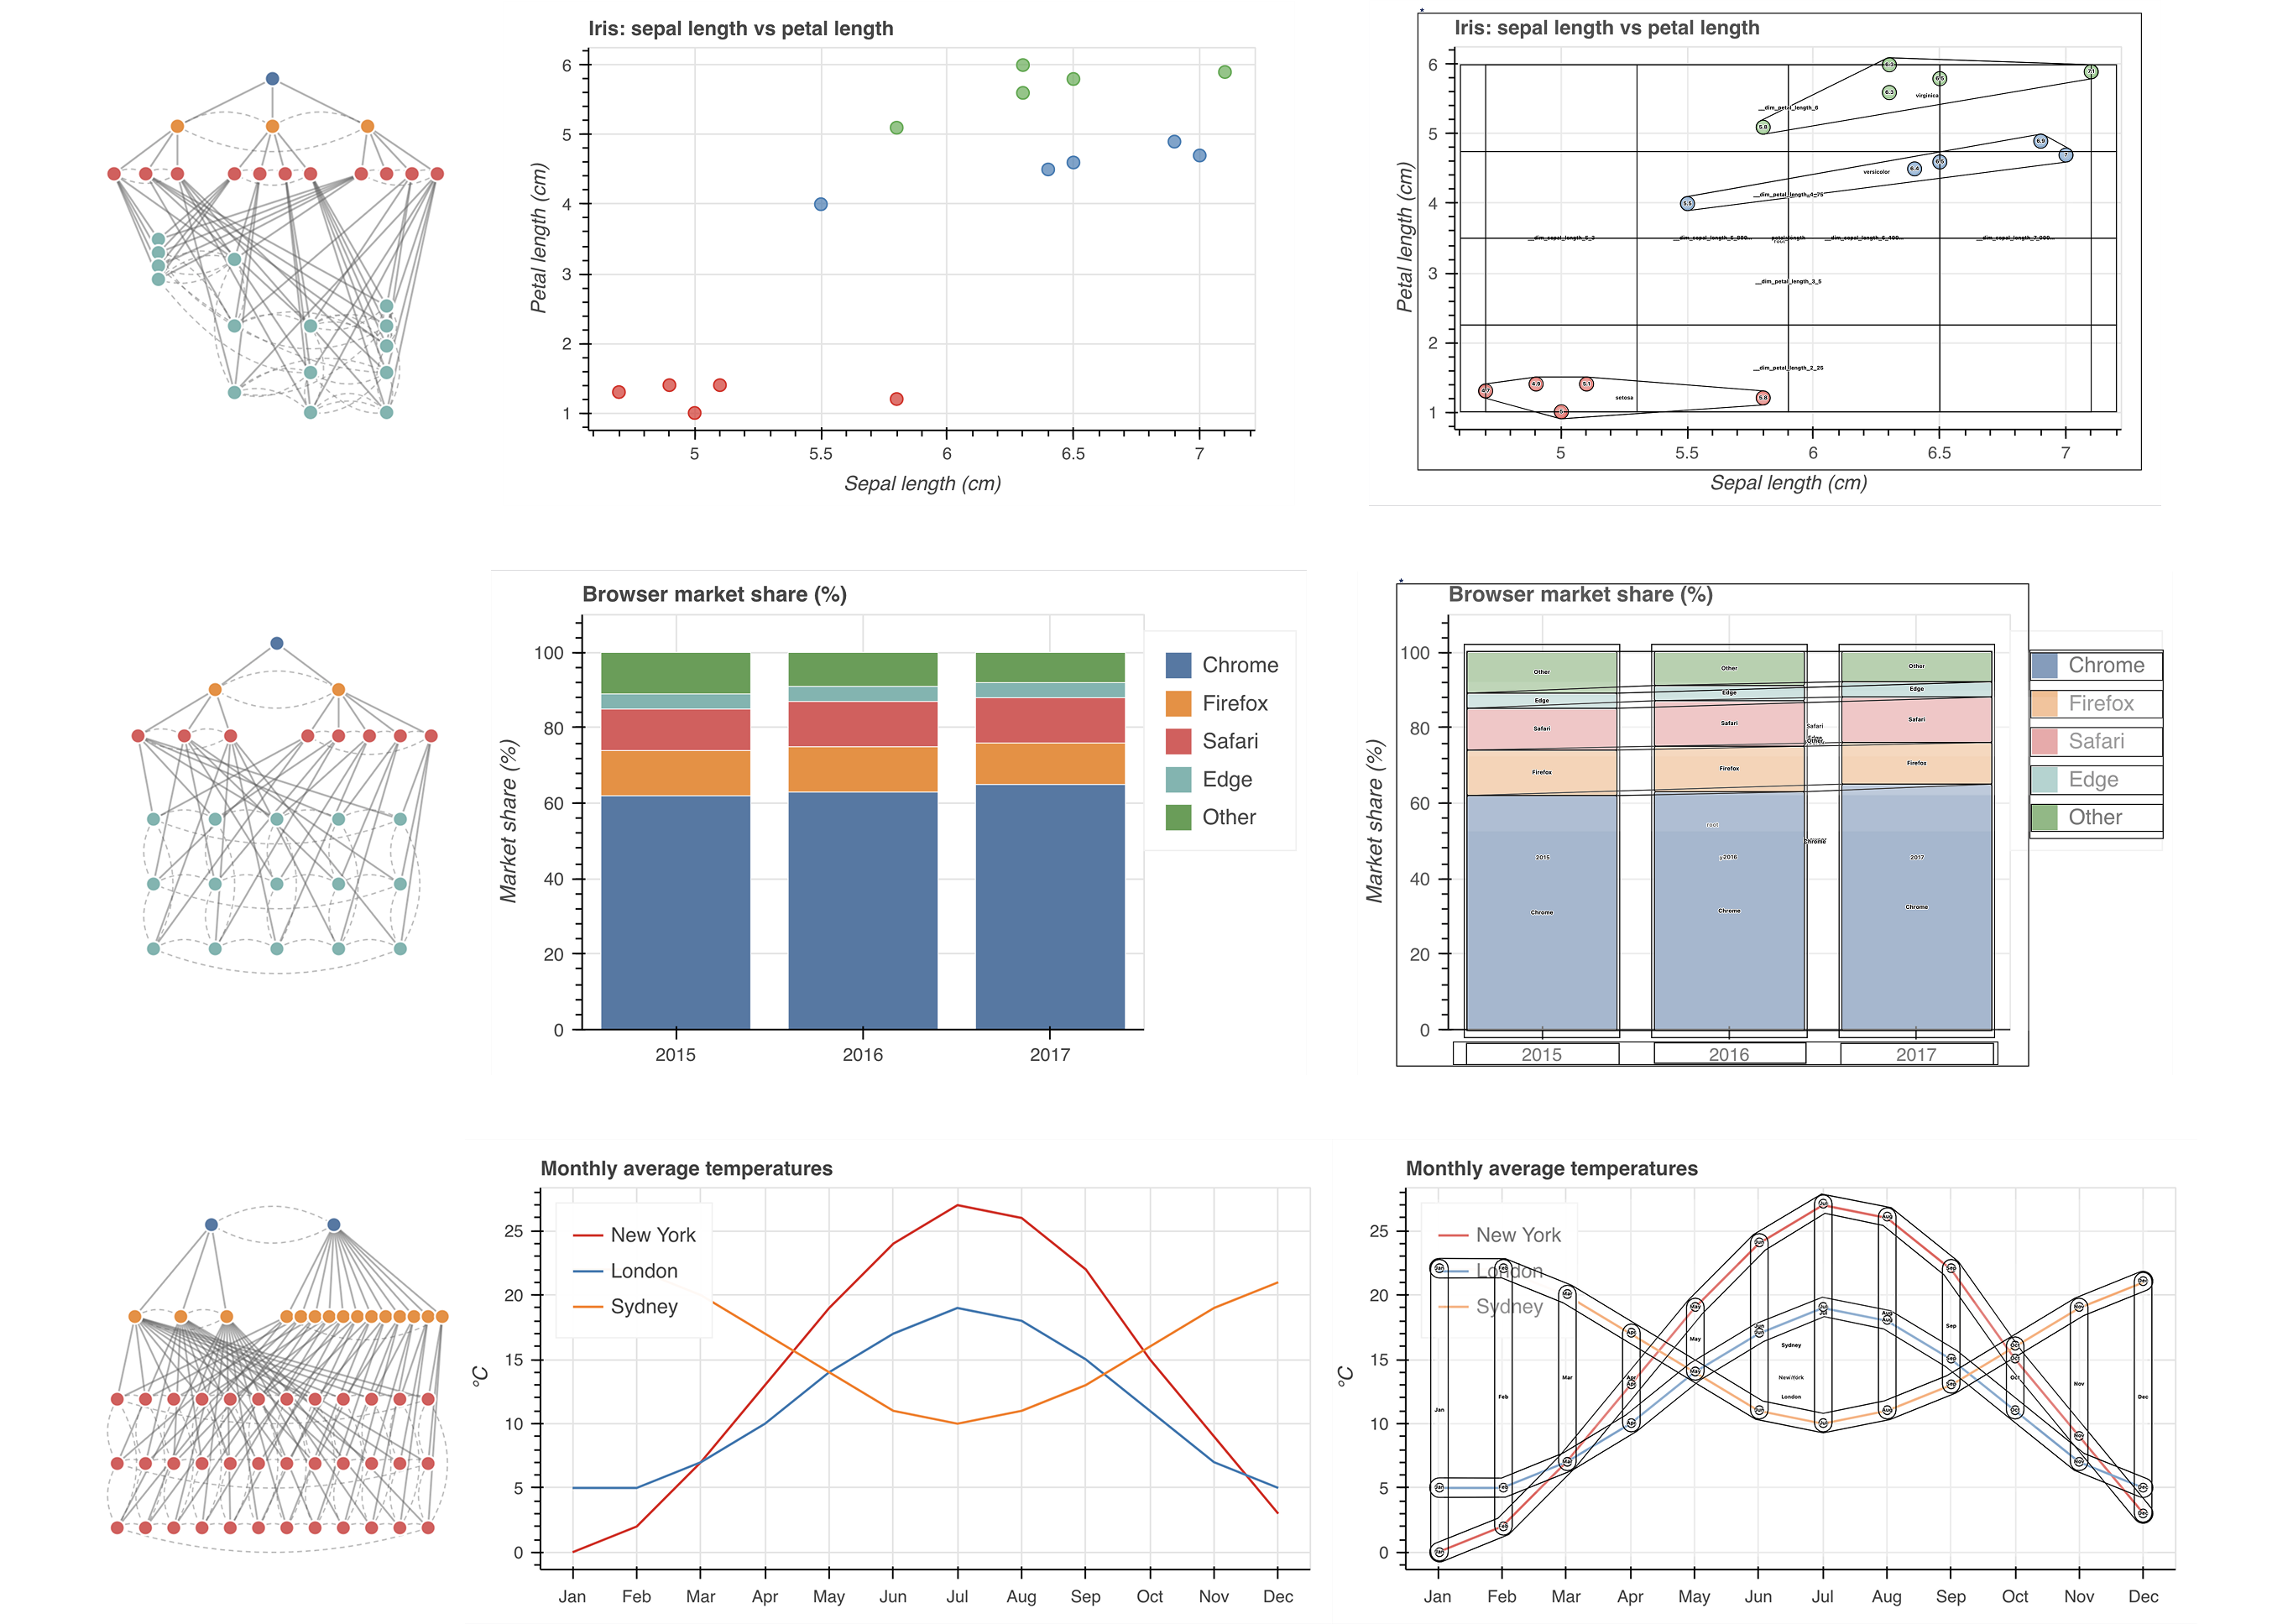
\includegraphics[width=\columnwidth, alt={A scatterplot, stacked bar, and line chart. Each has a graph next to it that shows nodes and edges. On the other side of each chart is a version of itself with grides, outlines, and marks that represent the various shapes and locations that the nodes and edges take over the chart's space.}]{figures/scaffold.png}
  \caption{%
  	Input data transformed into a navigable structure using the \textit{Dimensions API} and visualized with our \textit{Inspector} gadget (left). The input chart (middle). The navigable structure is transformed and drawn over the chart using the \textit{Scaffolding Engine} (right).%
  }
  \label{fig:scaffold}
\end{figure}

\textbf{Seeing the system, seeing the experience.} The editor is \textit{Skeleton}'s primary authoring environment (\Cref{fig:hero}) and presents two interlinked representations of the same navigation structure. A schema panel shows the structure as an abstract hierarchical tree layout that makes levels and parent-child relationships immediately readable. A graph canvas shows the same structure rendered as geometric elements positioned over the uploaded chart image, representing what an end user would encounter spatially. These two representations are bidirectionally linked: selecting a node in either view propagates the selection to the other, so practitioners can simultaneously hold in mind both the abstract topology of what is navigable and the spatial instantiation of where that navigation will live. The dual-view design makes visible a real conceptual divide between the system's model of navigation and a user's experience of it, one that practitioners recognize once they can see it, even without prior vocabulary for it.

\textbf{Leveraging visualization as a scaffolding engine.} Manually positioning leaf nodes over each data mark is the most mechanical step in the authoring workflow, and it scales poorly with dataset size. In our early pilot sessions, actually placing nodes in the canvas space was the slowest and most tedious part of the process. To address this, \textit{Skeleton} includes a scaffold tool (\Cref{fig:scaffold}) that automates spatial placement by repurposing Vega~\cite{Satyanarayan2017VegaLite} as a layout engine.

The scaffold renders a Vega chart specification to a hidden, off-screen container and extracts node positions via the library's internal scale and view APIs, using the rendering engine purely as a coordinate computation step: no actual chart is ever shown to the practitioner. Coincidentally, none of our co-designers were crafting visualizations using Vega or Vega-Lite (or derivatives), yet the Vega rendering engine could faithfully reconstruct every necessary mark position over the underlying, inaccessible data visualization provided to \textit{Skeleton}. 

Additionally, positions and outline strategies for category-level group nodes are computed from the leaf positions using geometric algorithms: a union of child node paths, a convex hull, a grid over numerical bounds, or a bounding rectangle. These designs were consistently produced as ideal treatments during co-design, so we chose them for our starting set of outline strategies.

The scaffold is optional and works by generating synthetic placeholder positions that practitioners can adjust manually. It dramatically improved authoring speed: in light pilot tests, a research team member completed a three-dimension structure without scaffolding in 8 minutes 22 seconds and with scaffolding in 56 seconds. A co-designer completed the task incorrectly (failing to account for one dimension's division nodes) in 13 minutes 7 seconds without scaffolding, and correctly in 2 minutes 44 seconds with it.

\textbf{Specifying token patterns, editing instances.} Selecting any node populates a properties panel with spatial properties (position, size, shape) and semantic properties (ARIA role, description, and a label template editor; \Cref{fig:label}). The label template allows practitioners to assemble the text a screen reader will announce at that node from tokens drawn from data fields, including aggregate statistics at group-level nodes and precise data values at leaf nodes~\cite{Jones2024}. Editing labels can apply to all nodes of the same type or to a single instance.

\begin{figure}[h]% specify a combination of t, b, p, or h for top, bottom, on its own page, or here
  \centering % avoid the use of \begin{center}...\end{center} and use \centering instead (more compact)
  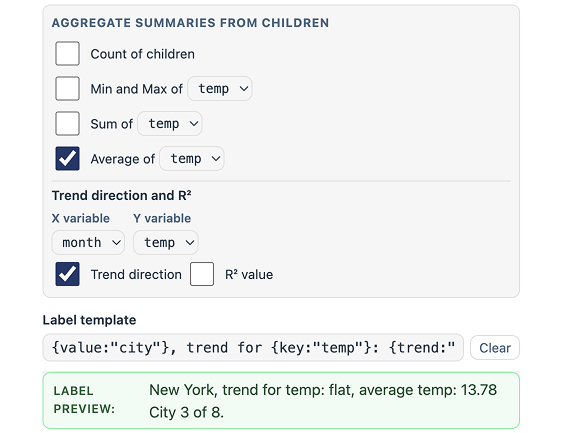
\includegraphics[width=0.7\columnwidth, alt={Label builder UI. Show interface options, label template filled with generic pattern-building text, and then a label preview shows output "New York, trend for temp: flat, average temp: 13.78, City 3 of 8. Long description of UI details: title "Aggregate summaries from children" unselected count of children, unselected min and max of dropdown with temp selected, unselected sum of dropdown with temp selected, selected average of dropdown with temp selected. "Trend direction and r squared options" x variable dropdown with month selected, y variable dropdown with temp selected, selected trend direction, unselected r squared.}]{figures/label_preview.png}
  \caption{%
  	Group label pattern builder, including an array of aggregate summary options, template formatter field, and preview.%
  }
  \label{fig:label}
\end{figure}

At the bottom of the semantic section, a live preview displays the full assembled announcement string in the exact form a screen reader would produce: role, semantics, group membership, and label combined into a single rendered output that updates in real time. Prior to this preview, understanding what would be announced at a given node required running a screen reader and navigating to it sequentially. In deeply nested structures, this meant spending several seconds listening to labels and drilling in. This was consistently the main point where bugs were produced and missed during our co-design work.

The preview makes text announcements inspectable as visible, editable objects. This surfaces a class of highly specific, low-level problems that code-only workflows leave invisible: redundancies in announced text, missing contextual framing, and label ordering and punctuation that affects comprehension and reading speed. Of all the authoring decisions \textit{Skeleton} exposes, label templates involve the most degrees of freedom and have the most direct bearing on the quality of the non-visual experience. Getting the structure right ensures navigability; getting the labels right determines whether navigation communicates anything meaningful.

\subsection{Test: Debugging Interaction Interactively}
\label{sec:testing}

The testing stage allows practitioners to navigate the structure they have built using the same keyboard input and navigation rules that assistive technologies would use, without leaving the tool. When a practitioner enters testing, the three Data Navigator modules are instantiated in sequence: the structure module rebuilds the navigation graph from the current configuration, the rendering module creates an HTML layer positioned over the chart image at each node's spatial coordinates, and the input module registers keyboard listeners for all navigation rules. The result is a live, keyboard-navigable structure. An event log records navigation events in order, letting practitioners verify that all nodes are reachable and that label sequences make sense when encountered serially rather than read simultaneously.

The abstract graph continues to display during testing. As the practitioner navigates, the focused node is highlighted simultaneously in the canvas (showing its spatial position over the chart image) and in the abstract graph (showing its structural position in the hierarchy). This parallel tracking makes the temporal traversal sequence visible, showing the order and path through which a user encounters nodes, so practitioners can verify at a glance both where focus is and what role it occupies. A text-chat mode is also available, in which practitioners navigate by typing natural language commands, motivated as a design by the Adobe collaboration (\Cref{sec:designsystem}), to explore interaction alternatives for mobile screen reader users.

The testing stage also served, during development, as the primary debugging interface for \textit{Skeleton}'s own data pipeline. Errors in position computation, label resolution, or structure generation that would propagate silently through code became visible the moment a node highlight appeared in the wrong location or a label read as undefined. A tool for making non-visual structure visible turned out to benefit from the same property during its own construction.

% \textbf{Accessible authoring.} \textit{Skeleton} faces a recursive design challenge: the tool itself must be accessible to practitioners who use assistive technologies. Our approach was shaped by CD2, who recommended ensuring that practitioners navigating \textit{Skeleton} with assistive technology could not become trapped inside a navigation structure they were actively editing. We implemented this as a deliberate constraint: during editing, keyboard navigation through the graph canvas is list-based, traversing nodes in sequence without exposing the full navigation graph to the assistive technology. The testing stage provides the richer navigational experience for practitioners who want to preview designed behavior using their own assistive technologies, separating authoring mode from testing mode as distinct interaction contexts. CD2 also raised unresolved questions: how should practitioners know when a structure is ready to test, and what does meaningful evaluation look like from the perspective of end users?

\textbf{Practice-based validation.} CD2, a subject matter expert who professionally evaluates interfaces for screen reader access and is familiar with other visualization navigation systems, used \textit{Skeleton}'s testing stage to evaluate navigation output across several chart types and dimension configurations: line charts (3 configurations), bar charts (2), stacked bar charts (3), and scatterplots (4). This evaluation followed a manual, systematic approach combining standards-based criteria with expert screen reader testing. Scatterplots required the most iteration, surfacing bugs in Data Navigator's core library that were then fixed. CD2 also recommended that we rely on list-based navigation while in the editor (before the testing stage) in case users build themselves into a keyboard trap.

\section{User Study}

Our co-design work followed an action research orientation: the research team was embedded in practitioner communities, and our system work was motivated by the problems those communities faced. This process generated the techniques and infrastructure that comprise \textit{Skeleton}, but we still needed to understand the impact our system had on visualization practitioners more broadly. Our co-designers were deeply familiar with the problem space, having spent months or years working on accessible navigation. We needed to understand what happens when practitioners who are \textit{not} embedded in this process design, author, and debug navigation structure visually: whether the representations we built are legible to them, whether the techniques change how they reason about accessible design, and what new questions or problems emerge when navigation structure becomes visible. These are empirical questions that required a study.

To evaluate how \textit{Skeleton} influences the way practitioners engage with accessible design, we conducted an in-situ interview study with 8 participants across visualization design, engineering, and research. The study was conducted remotely over video call, took approximately 45--60 minutes per session, and was approved by our IRB. Participants provided verbal consent at the start of each session. Video and audio were not recorded, however some participants consented to share the data/image they brought to the study as well as screenshots of their workflow; data collection was note-based throughout.

\subsection{Participants}

Participants were recruited through snowball sampling within the visualization and accessibility community, and through referrals from co-designers involved in our earlier collaborations. We asked each participant to self-report their primary work role (engineering, research, design, or student) and their existing level of accessibility expertise on a 1--5 Likert scale. We also asked whether the visualizations they build are ever bespoke, that is, custom rather than instances of a recognizable, standard chart type. This distinction mattered because bespoke visualizations represent an especially underserved case in accessible design tooling: no library pattern applies, and every navigation structure must be designed from scratch. Participants were not compensated.

\subsection{Procedure}

Each 45-minute session proceeded in four phases. Before the session, all participants were asked to prepare a chart image they were currently working on or had recently built, for use in the third phase.

\textbf{Phase 1: Introduction and demographics (5 minutes).} After obtaining verbal consent and recording a pseudonym, we collected self-reported role, accessibility expertise level, and whether the participant regularly builds bespoke visualizations.

% \textbf{Phase 2: Pre-tool reflection (10 minutes).} We showed participants an interactive bar chart and explained its interaction model: selecting a bar loads a new dataset. We then asked, in a short semi-structured interview, how they would make this chart accessible to a screen reader user, what decisions they would need to make, and what they considered hardest. Participants could diagram or write freely in Figma. This phase was a qualitative reference point, not a formal baseline: articulating their approach before using the tool made it possible to later ask what changed and why.

\textbf{Phase 2: Generic chart think-aloud~\cite{Alhadreti2018} (10 minutes).} Participants used \textit{Skeleton} on a provided bar chart and dataset of fruit counts (Apples, Pears, Nectarines, Plums, Grapes), asked to design an accessible navigation experience for a screen reader user with no instructions on how the tool worked. The tool loaded with a default structure having both a categorical dimension (\texttt{fruit}) and a numerical dimension (\texttt{count}) active. This default was intentionally problematic for two reasons: numerical navigation sorts by count value and groups data into subdivided ranges, producing a traversal order different than the visual layout an additional, largely unhelpful level in the hierarchy for such a simple chart. We observed how participants reasoned about what they saw and whether and how they noticed this extra dimension.

\textbf{Phase 3: Own-chart think-aloud (15 minutes).} Participants loaded their own chart image and attempted the same task, except they were also asked to explain their graphic to the research team (purpose, role, data, and domain). This phase was open-ended: charts ranged from standard types to bespoke visualizations, and the goal was to observe how participants reasoned about navigation structure when the context was their own work.

\textbf{Phase 4: Reflective interview (15 minutes).} We conducted a semi-structured interview in which participants reflected on their decisions in Phase 2 versus Phase 3, their experience with the generic versus their own chart, and their assessment of the tool's capabilities and limitations. We asked what felt possible or impossible, what they wanted to do that they could not, and what they found themselves thinking about that they had not considered in Phase 2.

\subsection{Analysis}

Notes from each session were compiled into a shared document. Participant quotes reported in the results are reconstructed from these researcher notes, not verbatim transcripts. We analyzed the data using a combination of thematic analysis~\cite{Braun2006Using} and affinity diagramming~\cite{Harboe2015}, iterating across both methods to surface recurring patterns while preserving the specificity of individual participant experiences. Analysis attended particularly to differences in how participants engaged with accessible design before and after using the tool, the range of input modalities and user scenarios they considered, and moments when participants reconsidered or wished to redesign their own visualizations.

\section{Results}

We organize our findings into five themes that emerged from thematic analysis and affinity diagramming across all eight sessions. Each theme captures a qualitative pattern in how practitioners engaged with accessible navigation design when its structure was made visible and manipulable. We report these findings descriptively and ground them in specific participant moments; interpretation follows in the Discussion.

\subsection{Seeing Navigation Made Structural Problems Legible as Design Problems}
\label{sec:results-legible}

The generic bar chart in Phase 2 loaded with an intentionally problematic default: both a categorical dimension (\texttt{fruit}) and a numerical dimension (\texttt{count}) were active, producing overlapping navigation structures with different traversal orders over the same data. This configuration is a poor design choice, arguably a design failure, but one that would be difficult to detect in code alone~(\ref{rq:R1s}, \ref{rq:R4s}).

Participants varied widely in how quickly they recognized the problem. P1 turned off the numerical dimension within seconds of seeing the editor, without commenting on it. Most participants, however, initially struggled to understand what they were seeing, remarking on the unfamiliar structure: ``what is this? what are these?'' when encountering the numerical divisions for the first time. P8 spent time trying to guess what the extra divisions represented but did not remove them during Phase 2, only realizing during Phase 3 that the additional dimension was ``probably bad.'' P2 and P5 expressed suspicion early: P5 asked, ``Is this too much data? This seems like way too much to just navigate through,'' and P2 noted, ``I feel like a lot of data points would be bad, yeah? Like, too many at once is bad?'' Both of these remarks were prompted by the visual density of the structure, not by navigating it.

The testing stage (\Cref{sec:testing}) proved critical for resolution. P4, P5, and P7 each removed the extra dimension only after navigating the structure with keyboard input in testing mode, where the traversal sequence made the redundancy experientially apparent. In total, five of eight participants resolved the problem during the session: P1 and P2 during editing, and P4, P5, and P7 after testing.

Beyond the intentional default, participants identified other problems through visual inspection. P8 reacted to a generated node name: ``Okay dim\_fruit node\ldots that is horrible, what is that?'' During Phase 3, P7 looked at the edges of their multi-line chart and asked, ``are all these bad? Is it bad that I don't even really know what the takeaway of this [structure] is?'' P3, seeing a full hierarchy for their own simple six-item bar chart (during Phase 3), concluded ``I should just skip the root and grouping and go straight to the data. This seems like too many steps.'' In each case, the visual representation of their navigation structure motivated judgment about potential negative design qualities.

\subsection{Practitioners Developed a Designerly Interest in What Constitutes Good Navigation}
\label{sec:results-designerly}

The most pervasive pattern across sessions was that participants began asking design questions about navigation quality, unprompted by any instruction or guidance from the research team~(\ref{rq:R2s}). These questions went beyond identifying errors: participants wanted to know what \textit{good} navigation would be for their charts.

% They also considered hierarchical depth: ``I don't know if root is important\ldots my inclination is to put this up front or above, but it does feel superfluous for this.''

P2, working through the bar chart in Phase 2, deliberated over boundary behavior: ``Loop back or stop? I don't think there is a right way. I will just pick \textit{fruit} for now and \textit{loop} and see what this does.'' P6, who brought a bespoke flower visualization, wondered how to translate the affective quality of their chart: ``I think my visualization should be more about the vibes, but I don't know how to make the alt text have good vibes. What is \textit{fun}?'' P4 asked fundamental questions about the interaction model itself: ``Why do screen readers and keyboards have to work this way? Do people like that?\ldots why do we navigate?'' And later after testing, P4 concluded, ``I bet we should make this \textit{faster}'' before cutting out the additional numerical dimension in Phase 2.

% ``What are you trying to convey\ldots what are you trying to communicate?'' They connected this to an argument about level of detail:

Several participants engaged with the concept of narrative and flow. P8 articulated this as a question about the goal of the visualization: ``sometimes I want a big picture, not precision. I may want to drill down a little\ldots'' and observed that ``we think too much in terms of components\ldots sometimes accuracy isn't the actual goal, it's getting a general sense of something.'' P4, upon discovering that \textit{Skeleton} supports text-based input, asked, ``How do you make that good, though? Like chatGPT, or do people want to, like, interact with the chart [elements]?'

During the interview, several participants explicitly requested guidance. P1, P2, P3, and P6 wanted to see examples of well-designed navigation experiences. P1, P3, P4, P5, P6, and P7 wanted embedded guidelines within the tool. P2 and P4 actually used web search to look for ``chart navigation for accessibility guidelines'' (P2) and ``accessible viz screen reader design'' (P4). P3 was interested in automation and heuristics that could suggest reasonable defaults. These requests are consistent with the pattern~(\ref{rq:R2s}): practitioners who could see the design space wanted orientation within it.

\subsection{Iteration Was Substantive, Self-directed, and Concentrated on Semantics}
\label{sec:results-iteration}

Every participant iterated on their navigation designs, and this iteration was neither perfunctory nor prompted by the research team~(\ref{rq:R4s}). Participants revisited decisions, revised configurations, and in some cases restructured their entire approach after encountering their design in a new stage of the tool.

The most sustained iteration concerned labels and text announcements. Every participant spent the largest share of their authoring time in the label template editor (\Cref{fig:label}), editing the text that a screen reader would announce at each node. This editing was granular: participants wrote full sentences, rearranged the order of data tokens, debated whether to include field keys alongside values or values alone, experimented with how to name groups and individual elements, and considered the length and density of the resulting announcements. At the division and dimension levels, some participants added multiple aggregate statistics (count, sum, average, range, trend) and then returned to trim them. P2, for instance, edited data point labels, left them, and returned to revise them two additional times: ``This label is way too complicated, I think.'' These label iterations were small, fast, and frequent, and they reflected an intuitive grasp of the importance of the textual tokens that constitute a screen reader user's primary interface to data. 

A second, distinct pattern of iteration emerged around testing. The editor displays all navigation nodes simultaneously, showing the full structure at a glance. The testing stage (\Cref{sec:testing}), by contrast, shows only the currently focused node, highlighting it in the canvas one at a time as the practitioner navigates. This difference consistently prompted participants to revise. Several returned to the editor after testing to adjust group node outlines, because outline strategies that looked distinct when displayed simultaneously (such as bounding rectangles vs. convex hulls) became harder to differentiate when encountered one at a time. Others adjusted their dimension configurations: P3 and P5 restructured their dimensions after testing, and P4, P6, and P8 experimented with different key bindings and navigation rules. P2 used the testing stage specifically to identify labels that needed revision at the dimension and division levels. In these cases, testing was not only treated as a bug-finding activity but also as a way to encounter, reason about, and then improve a design that had looked adequate in the editor but felt inadequate in sequential traversal.

The most extensive iteration came from P1, who returned to the preparation wizard after reaching the testing stage and re-took the entire wizard from scratch. Seeing the full structure in testing motivated them to re-evaluate their earliest decisions. They reduced their navigation from three dimensions to one, producing a navigation experience they described as deliberately minimal. In the reflective interview, P1 explained that they had been thinking about trimming excess, joking that they were ``working on a data-to-word ratio.''

The scaffolding tool shaped the pace and character of these iterations. Participants who used the scaffold (\Cref{fig:scaffold}) generally required only minor manual adjustment of node positions, spending one to two minutes refining placements in-aggregate before moving on. Iteration on spatial layout was primarily about the appearance of group-level outlines rather than individual node positions: because the scaffold computed leaf positions from the chart's encoding, the main remaining spatial decision was how division and dimension nodes should visually indicate their grouping. When participants returned to scaffolding, it was most often because they wanted to change the chart type used for coordinate computation or to try a different group outline strategy.

\subsection{Seeing Navigation Prompted Practitioners to Reconsider the Architecture of Their Own Charts}
\label{sec:results-reconsider}

An unexpected finding was that working with \textit{Skeleton} prompted several participants to question the design of the visualization they had brought, not just the navigation structure they were building over it~(\ref{rq:R4s}). Five participants (P4, P5, P6, P7, P8) expressed a desire to simplify their own charts after seeing what the corresponding navigation structure required. Three (P1, P5, P6) considered whether a different chart type might serve the same communicative goal with a simpler navigational architecture. And in 2 cases (P1, P6), participants questioned whether a chart was the right medium at all.

P5, who brought a scatter plot with over two thousand data points, initially tried to build a navigation structure over the full dataset, recognized that the result was unmanageable, and then asked: ``do I even need visualization?'' They went on to wonder whether the information could be communicated as ``a few sentences or like, some data [users] can prompt'' (referring to using a large-language model). P6, who brought a bespoke flower visualization in which each petal encoded a different variable, initially tried to express the chart's full complexity in navigation (grouping by flower and then navigating by petal) but then reversed course: ``okay, what if we actually just treat this like a bar chart?'' Using the scaffold tool, they produced a simple list-style navigation that worked well for their data, and reflected: ``my visualization has a lot, but actually, this could be pretty easy to navigate, I think.'' P6 also wondered whether there was a non-chart way to ``tell their story,'' and in further discussion described something closer to a scrollytelling article or guided walkthrough than a single interactive chart.

\begin{figure}[h]% specify a combination of t, b, p, or h for top, bottom, on its own page, or here
  \centering % avoid the use of \begin{center}...\end{center} and use \centering instead (more compact)
  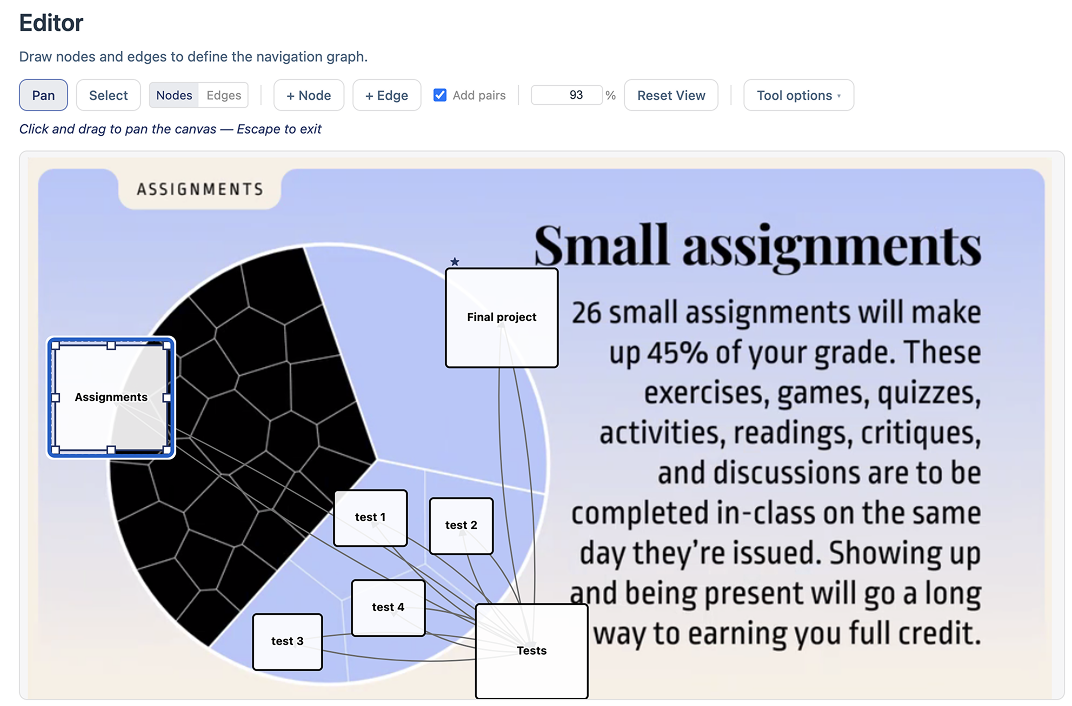
\includegraphics[width=\columnwidth, alt={A voronoi pie chart with a large slice emphasized. A large text caption reads, Small assignments: 26 small assignments will make p 45\% of your grade. These exercises, games, quizzes, activites, readings, critiques, and discussions are to be completed in-class on the same day they're issued. Showing up and being present will go a long way to earning you full credit.}]{figures/voronoi_pie.png}
  \caption{%
  	Re-creation of P8's moment of realization, placing nodes manually: not every element in their voronoi pie chart \textit{should} be navigable.%
  }
  \label{fig:voronoi}
\end{figure}

P8's case was the most striking. They brought a voronoi pie chart (\Cref{fig:voronoi}) used to communicate to students that 26 assignments make up 45\% of their grade, the largest slice of the pie. Working through \textit{Skeleton}, P8 first considered making all 26 voronoi cells navigable, then considered making only the three main slices of the pie navigable, and then questioned whether navigation was needed at all. The ``point of this,'' as they described it, was to communicate a single ratio; students did not need to traverse individual cells to understand it. P8 concluded that well-written alternative text was sufficient for the screen reader experience and chose not to build a navigation structure. They also reflected on the design of the visualization itself, concluding that the voronoi treatment served a visual purpose (it is visually striking) that was separable from the informational purpose (communicating a grade breakdown). They kept the visual design and simplified the non-visual experience accordingly.

\subsection{Experiencing Keyboard Navigation Surfaced a Broader Range of Users and Input Technologies}
\label{sec:results-keyboard}

The testing stage (\Cref{sec:testing}) provided what was, for most participants, their first experience of keyboard navigation through a data visualization. Only three participants (P1, P2, P8) reported prior experience using a screen reader, and only two (P1, P8) had previously navigated a visualization using keyboard input alone. Yet during the study, every participant navigated using a keyboard.

Several participants responded to this experience with genuine engagement. P4 reacted with enthusiasm: ``Woah, this is incredible. Wait, what other visualizations can do this?'' and later, ``Maybe you could make a visualization game, where you can move around the data?'' P7 said, ``I love this. I want to make charts with this.'' P5, who had not previously encountered keyboard-navigable charts, said, ``I didn't know you could do this.'' These reactions were not about the tool; they were about the interaction modality itself, about the experience of traversing data spatially using directional input.

The experience also expanded participants' sense of who these structures serve~(\ref{rq:R2s}, \ref{rq:R4s}). P8 adjusted a node's spatial dimensions and said, ``Let's make the hitbox as big as possible here\ldots for my neighbor with Parkinson's to click these,'' treating the navigation structure as relevant to motor accessibility, not only screen reader access. P3, observing the visual focus indicators that appeared during scaffold-based placement, remarked that ``this is for more people than [someone] blind,'' recognizing that sighted keyboard users and users with partial vision also rely on visible focus states. During the interview, P4 asked sustained questions about what kinds of technologies different people with disabilities use, and P4 and P7 both asked why focus indication was designed to be visible rather than invisible.

P4's curiosity extended to alternative input modalities. Upon learning that \textit{Skeleton} supports text-based navigation and (due to leveraging Data Navigator) also supports a wide array of other input modalities, they asked, ``Can you talk at it, too? Is that what some people do?'' and followed up with, ``How cool is that? How do you make that good, though?'' P8 raised a concern about discoverability in the current interaction model: ``I've never used j or w to drill out, always shift arrow or option arrow\ldots'' and worried that a user might not know how to exit a nested level. These observations reflect an broad mental model of the user, from an abstract ``screen reader user'' to a person with multiple capabilities, preferences, and interaction patterns~(\ref{rq:R2s}).

\section{Discussion}

\subsection{Visibility as a Precondition for Iteration}

The central finding of this work is not that \textit{Skeleton} taught sighted practitioners how to design accessible navigation, but that it gave them something to react to. When navigation structure was invisible, our co-designers would only seek to verify whether navigation followed our design documentation. Once visible, questions shifted to whether it was good, why, how it could be improved, and what else it could do. Visibility encouraged iteration, and iteration is enabled continuous design improvements.

This mechanism is consistent with Sch\"on's account of reflective practice~\cite{Schon1996Relective}: designers iterate by externalizing a representation, perceiving its properties, and responding to what they see. The representation talks back, and the designer adjusts. But this loop requires a representation. In our co-design work, we assumed that the gap was hand-off between design and development, and the slow process of manual verification. Instead, the gap is that development was not participating in, and encouraging, further design reflection. In a developer's code-only workflow, navigation structure has no externalization that supports this kind of perceptual engagement. A practitioner can read the code that specifies a navigation graph, but they cannot see the graph, cannot perceive its topology at a glance, cannot notice that a label is redundant or that a hierarchy is too deep by looking at it. The reflective loop is disrupted and occluded at the first step.

\textit{Skeleton} encourages this loop by rendering navigation structure in a form that supports the same kind of perceptual judgment that visualization practitioners already apply to every other aspect of their work. The results show what happened when this loop was available: every participant iterated, substantively and self-directedly (\Cref{sec:results-iteration}). They revised labels repeatedly, restructured dimensions after testing, adjusted group outlines when sequential traversal revealed problems that simultaneous display had hidden. P1 restarted the entire preparation wizard after seeing their structure in testing mode. These are not the behaviors of practitioners following a specification; they are the behaviors of practitioners negotiating with a design material.

The co-design work reported in \Cref{sec:codesign} provides complementary evidence: in each collaboration, sighted practitioners naturally reached for visual representations when reasoning about navigation, through node-link diagrams in Figma, schema sketches in Miro, and annotated wireframes on paper. They were already thinking visually about non-visual structure; the development tooling simply had not caught up. This has a practical implication for the broader field: if sighted authors depend on visibility, then any authoring workflow that keeps navigation structure invisible limits design iteration. Making structure visible does not guarantee good design, but it is a precondition for the kind of sustained, judgment-driven refinement that good design requires.

% This has a practical implication for the broader field of accessible visualization authoring. If sighted authors depend on visibility, then any authoring workflow that keeps navigation structure invisible produces barriers that limit the accessibility of design iteration. We believe that the quality ceiling may not be set only by practitioner skill or motivation but by also be influenced by the absence of a readily legible feedback loop. Making structure visible does not guarantee sighted authors will produce good design, but it is a precondition for the kind of sustained, judgment-driven refinement that good design requires.

\subsection{From Compliance to Design}

% A consistent pattern across the accessibility literature is that practitioners frame accessibility as a compliance problem: a set of requirements to satisfy, a checklist to complete, a legal or institutional obligation to meet~\cite{Joyner2022Wild, Sharif2024Challenges, Elavsky2022Chartability}. The framing matters because compliance and design orient practitioners toward fundamentally different activities. Compliance asks: ``does this pass?'' Design asks: ``is this good?'' These questions lead to different behaviors, different kinds of attention, and different ceilings on quality.

% The results suggest that \textit{Skeleton} produced a shift from the first orientation to the second, at least partially and temporarily, across participants. The evidence for this shift is not a single moment but a pattern of behavior. In Phase 2, when first using the tool, participants' initial instincts clustered around familiar compliance-oriented responses: provide alternative text, follow guidelines, ask an expert what to do. Six participants explicitly requested embedded answers or examples of ``correct'' navigation designs, and two searched the web during the session for accessibility guidelines related to chart navigation. These are reasonable responses, but they reflect an orientation toward external authority rather than independent design judgment.

% What changed was not that participants stopped wanting guidance. They continued to want it. But alongside that desire, they began doing something that compliance framing does not produce: they encountered complexity, difficulty, their own lack of knowledge, and then \textit{iterated}. They wrote labels, revised them, and revised them again. They tested traversal sequences and returned to restructure dimensions. They adjusted and re-adjusted group outlines after encountering them one at a time in testing mode. They debated boundary behavior, hierarchical depth, and how much information to surface at each level. They doubted themselves. They tried new ideas. This sustained, self-directed refinement when one recognizes problems is the behavioral signature of design, not compliance. A practitioner working from a checklist does not revisit a label three times to get the phrasing to sound just right. A practitioner designing an experience does.

% P4 articulated this shift directly in the reflective interview: ``I'd love to have someone blind actually just with me while I make this, but I also understand that I should learn what makes a good experience too.'' The statement captures both orientations simultaneously: the desire for expert guidance and the recognition that the practitioner's own judgment matters when answers are scarce. And what \textit{Skeleton} provided was not answers but a medium in which design questions could be asked and worked through. The tool did not argue practitioners into treating navigation as a design problem. It gave them a representation that made design questions visible, and they responded by designing.

% This distinction has implications beyond our specific tool. If a compliance-to-design shift for sighted authors is supported by having a visible, interactive representation of non-visual elements, then the widespread treatment of accessibility as a compliance activity may be partly a consequence of tooling that offers no legible, manipulable design surface. Auditing frameworks and automated validators are valuable, but they are \textit{evaluative} tools, not \textit{authoring} tools. They tell practitioners whether something passes; they do not help practitioners reason about whether it is effective or appropriate. The field needs both kinds of tools, and the authoring side remains underdeveloped.

A consistent pattern across the accessibility literature is that practitioners frame accessibility as a compliance problem: a set of requirements to satisfy, a checklist to complete, a legal or institutional obligation to meet~\cite{Joyner2022Wild, Sharif2024Challenges, Elavsky2022Chartability}. The framing matters because compliance and design orient practitioners toward fundamentally different activities. Compliance asks: ``does this pass?'' Design asks: ``is this good?'' Our results suggest that \textit{Skeleton} produced a partial shift from the first orientation to the second. Participants' initial instincts clustered around compliance-oriented responses: provide alternative text, follow guidelines, ask an expert. But alongside that desire for guidance, they began doing something compliance framing does not typically produce: they encountered complexity and then \textit{iterated}. They revised labels repeatedly, restructured dimensions after testing, debated boundary behavior and hierarchical depth. This sustained, self-directed refinement is the behavioral signature of design, not compliance. As P4 put it: ``I'd love to have someone blind actually just with me while I make this, but I also understand that I should learn what makes a good experience too.''

The shift extended beyond the non-visual experience itself. As reported in \Cref{sec:results-reconsider}, five participants reconsidered the design of the visualization they had brought, not just the navigation structure overlaid on it. Making the accessibility consequences of visual design choices visible prompted practitioners to question whether a different chart type, a simpler encoding, or a non-chart medium might better serve their communicative goals. This interrelation between non-visual and visual design suggests that the widespread treatment of accessibility as a compliance activity may be partly a consequence of tooling that offers no legible, manipulable design surface. Auditing frameworks are valuable, but they are \textit{evaluative} tools, not \textit{authoring} tools. The field needs both.

\subsection{Bespoke Visualizations as an Unaddressed Accessibility Research Problem}

% \textit{Skeleton} is designed to work with any 2D image surface, not only standard chart types. But the study revealed that bespoke visualizations, those that do not conform to recognizable chart grammars, surface design questions that no current tool or research adequately addresses.

% P6's flower chart and P8's voronoi pie chart both illustrate this gap. P6's visualization encoded multiple variables across petals of individual flowers, a representation with no standard navigational analog. Their solution was pragmatic: they treated the chart as a bar chart for navigation purposes, using the scaffold tool to produce a simple list-style traversal. This worked well enough for their data, but they got lucky. Additionally, this solution required the participant to perform a conceptual translation that the tool did not intend to support. P8's voronoi pie chart posed a different version of the same problem: the visual form was chosen for its visual impact, not for its informational structure, and the most appropriate accessible representation turned out to be no navigation at all, just well-written alternative text. Both cases required practitioners to reason about the relationship between a visualization's visual form and its communicative purpose, a distinction that standard chart-type-oriented tooling does not surface. \textit{Skeleton} may have helped them each reach a working solution, but in both cases, they chose solutions that \textit{Skeleton} was not designed to assist with.

Diagrams, infographics, and data-driven illustrations are often one-off, custom designs with bespoke symbols, layouts, and visual languages. These representations are increasingly common in journalism, scientific communication, personal projects, art, and public-facing data work, and they represent the cases where accessibility-focused tools are needed most and available least. \textit{Skeleton}'s image-based workflow (upload any 2D image, place nodes manually) provides a starting point, but the study made clear that bespoke visualizations need more than node placement. They need support for reasoning about what navigational structure (if any) is appropriate when no template applies, a research problem that remains largely unexplored.

\subsection{What Visualization Owes Accessibility}

% We began this paper with a provocation: how might the discipline of visualization help the discipline of accessibility? The results give a more specific answer than we had at the outset. Visualization is a discipline built on making abstract structure perceivable and manipulable. Its core methods, grammars of encoding, direct manipulation interfaces, and iterative feedback between representation and understanding, are not specific to visual perception. This paper applies them to a structure that has, until now, resisted inspection: the navigation graphs that govern how assistive technologies traverse data.

% They are methods for rendering structure inspectable. 

Our approach, to make visual non-visual experiences, should not be limited to data visualization's own accessibility challenges. Navigation structure is a foundational component of accessible experience across domains: PDF and document reading order, web page structures, and software application layouts. In each of these areas, sighted practitioners author non-visual experiences without visual feedback, and in each, the same gap between design intent and verifiable outcome constrains quality. Testing is slow, error prone, and requires expertise in assistive technology use. Visual tooling for authoring, inspecting, and debugging non-visual structure~(\ref{rq:R3s}) is a tractable and high-value problem across application domains.

There is also a deeper question about what visibility can accomplish in principle. Work on multi-modal authoring environments has argued for de-centering visual representation and treating modalities as equal partners in the design process~\cite{Zong2024}, an important ethical commitment. \textit{Skeleton} does not do this: it re-centers visual representation as the medium through which sighted practitioners engage with non-visual structure. We believe this is justified pragmatically, because sighted authors need to articulate navigation design in their own perceptual language before they can reason about it at all, and this paper provides evidence that they do. But articulating a design in one's own language is not the same as understanding how it will be experienced in someone else's. The structures participants built during our study were never evaluated by blind users, and visibility alone cannot substitute for that evaluation. The risk we want to name is that making non-visual structure visible to sighted practitioners could be mistaken for making it \textit{understood}, when in fact it makes it \textit{designable}, a real but bounded gain. The fuller design process requires collaboration with disabled users, not as an occasional supplement but as a regular practice. \textit{Skeleton} can make that collaboration more productive by giving both parties a shared representation or space of translation between representations, but it cannot replace it.

% Efforts such as the Accessibility Object Model (AOM) aim to provide programmatic access to accessibility semantics in browsers, though progress has been slowed by privacy concerns around assistive technology detection. Regardless of how specific standards efforts resolve, the broader principle holds: 

% This is a real boundary of the approach: making an artifact visible and designable for sighted practitioners is not the same as evaluating it from the perspective of disabled users. The former is what this paper addresses. The latter requires a different methodology, one that brings disabled users into the evaluation and authoring process as participants and co-designers.

What visualization owes accessibility, then, is not simply better output but authoring tools that better stimulate reasoning, both individually and collaborative, about design.

\section{Limitations and Future Work}

\textit{Skeleton} makes navigation structure visible to sighted authors, but it cannot reassure those authors whether the structure they have built is good for the people who will use it. The tool surfaces design questions; it does not answer them. Several participants asked what constitutes good navigation, and \textit{Skeleton} had nothing authoritative to offer. Our study with sighted practitioners evaluated whether making navigation structure visible stimulated design consideration, not whether the designs sighted practitioners produced were actually good. These are related but distinct questions, and the second remains open. CD2's expert screen reader evaluation of \textit{Skeleton}'s navigation output (\Cref{sec:testing}) provided practice-based validation for several common chart types and surfaced concrete bugs, but this evaluation was neither comprehensive nor controlled: many configurations remain untested, and expert review is not a substitute for evaluation with a broader population of end users.

Additionally, we treated \textit{Skeleton} as a design probe~\cite{Hutchinson2003TechnologyProbes, Hammad2024GameAware} rather than comparing it to a controlled condition: the goal was to elicit qualitative insight about how the tool elicits engagement, not to measure performance differences. 

Our approach using \textit{Skeleton} as a design probe only with sighted participants is both a limitation and, we believe, the right sequencing: \textit{Skeleton} improves the intentionality and iterability of what sighted practitioners produce, which is a necessary precondition for a subsequent evaluation or future collaborative design work between sighted and blind authors. Further research and evaluation should close this loop, ideally to engage how mixed-ability teams co-design multi-modal data experiences.

% through co-design sessions that bring blind and sighted practitioners together in a shared authoring environment.

% Additionally, recruitment through snowball sampling within our professional network and co-design community introduced selection bias: participants had substantially higher accessibility interest and expertise than the broader practitioner population. This may limit generalizability, though we note that designing for engaged, knowledgeable practitioners is itself a legitimate goal, as these are precisely the users whose work shapes what others inherit. 



% This framing is intentional but means the findings reflect the tool under researcher-accompanied use with a prototype, and may not replicate in independent deployment of a more complete system.

\textit{Skeleton} is also a prototype with substantial work remaining. Not within the scope of the paper, but our participants provided ample feedback on the functionality of the prototype itself. The most urgent gap is export functionality: practitioners can design and inspect navigation structures in the tool but cannot yet produce deployable output.

% Beyond export, we plan to add design guidance, both written and illustrative. The design-quality questions participants raised during the study, from how to evaluate traversal order to whether a hierarchy has the right depth, point toward a broader system of embedded accessibility guidance that does not exist in any current tool. How to provide guidance without 

% Following the co-design and study work reported here, we built two applied artifacts grounded in what we learned. For the open-source Bokeh community, we developed a wrapper implementing six common navigation patterns, including basic bar, stacked bar, line, cross-navigable line, grouped scatter, and spatial scatter, providing reusable scaffolding for chart types that appeared most frequently in practitioner workflows. For the Adobe React Spectrum Charts collaboration, we built a text-based navigation interface supporting natural-language interaction via an LLM, providing a mobile-friendly alternative to keyboard navigation for the chart components we co-designed. Both artifacts remain works in progress and are released as open source alongside this paper.

\section{Conclusion}

Accessible navigation structure has long occupied an awkward position in visualization practice: known to matter, difficult to design, and invisible to the people responsible for building it. The invisibility was not incidental. Without a way to see what they were making, sighted practitioners could not catch errors, could not iterate, and could not develop the kind of considered judgment that good design requires. Accessibility remained downstream of every other decision not because of any single failure, but because the authoring conditions did not support anything else.

\textit{Skeleton} demonstrates that those conditions can be changed. Making navigation structure visible and manipulable, as an interactive graph rendered over the spatial layout of a real visualization with live label previews and testable traversal, shifted how practitioners engaged with and reasoned about accessible design. They began asking qualitatively different questions than someone seeking compliance: whether the features and design of their structure was good, despite not having readily available answers. 

If any conclusive take-aways can be gleaned from this project: for researchers interested in engaging accessibility, this would mean future projects might explore translational spaces between visuals and non-visuals that help sighted partners engage blind designers. For practitioners who build, design, or audit this would mean that more visualization is needed in current tooling, to enhance and make multi-modal existing non-visual methods of authoring and evaluation.

What the paper leaves open is more than what it closes. We used \textit{Skeleton} as a design probe with sighted practitioners; we did not evaluate the navigation structures they produced with the end users those structures are meant to serve. And the broader disciplinary conversation, about what visualization research owes accessibility and what methods might transfer between them, has more questions than answers. We offer \textit{Skeleton} not as a solution to these problems but as evidence that engaging them directly, with the full weight of visualization's methodological tradition, is both possible and fruitful.

\part{Interaction: Exploring New Possibilities for Blind Data Science}

\chapter{\textit{Cross-perception}: Rethinking Input Design Towards Blind Analytical Interaction}

\noindent\rule{16cm}{0.4pt}
\begin{quote}
This chapter was adapted from my paper, currently under review with IEEE VIS:
\begin{adjustwidth}{1cm}{}
% \-\hspace{2cm}
F. Elavsky, Y. Li, J. Jang, L. Nadolskis, P. Carrington, and D. Moritz, ‘\textit{Cross-Perception}: Rethinking Input Design Towards Blind Analytical Interaction’, \textit{IEEE Transactions on Visualization and Computer Graphics}, 2026.
\end{adjustwidth}
\end{quote}
\noindent\rule{16cm}{0.4pt}

\section{Abstract}

Interactive visualization research has produced a rich repertoire of interaction techniques (brushing, linking, and cross-filtering chief among them) that accelerate exploratory data analysis for sighted users. And accessible visualization research has made substantial progress on making data perceivable and navigable for blind users. Yet what remains largely unaddressed is the \textit{analytical} tier of blind interaction: the capacity to actively filter, conjecture, and test hypotheses through direct data manipulation. In existing systems that accomplish interactive, analytical tasks, users predominantly query text or sequentially navigate across discrete units of information, paradigms which focus the user on one piece of information at a time. These experiences limit a user's ability to rapidly explore and interrogate multiple dimensions within a dataset simultaneously. To target this analytical gap, we introduce \textit{cross-perception}, an interaction technique that adapts cross-filtering for non-visual, tactile interaction. \textit{Cross-perception} enables coordinated tactile brushing over one data space to produce perceptible computational output in a separate, linked space, without requiring serial navigation between them. We instantiate \textit{cross-perception} in the \textit{cross-feelter}, a prototype hardware device with dual motorized faders, and evaluate it against screen reader methods in a within-subjects study with 15 blind participants, 7 of whom have professional data expertise. Cross-feelter substantially improves exploration speed (+90\%), query generation (+188\% computational, +54\% spoken), enjoyment, and reduces anxiety (particularly for participants without prior data expertise). We discuss implications for interaction design in accessible visualization and propose \textit{cross-perception} as a framework for a broader class of non-visual, analytically-oriented data interaction techniques.

\section{Overview}
\begin{figure}[h]% specify a combination of t, b, p, or h for top, bottom, on its own page, or here
  \centering % avoid the use of \begin{center}...\end{center} and use \centering instead (more compact)
  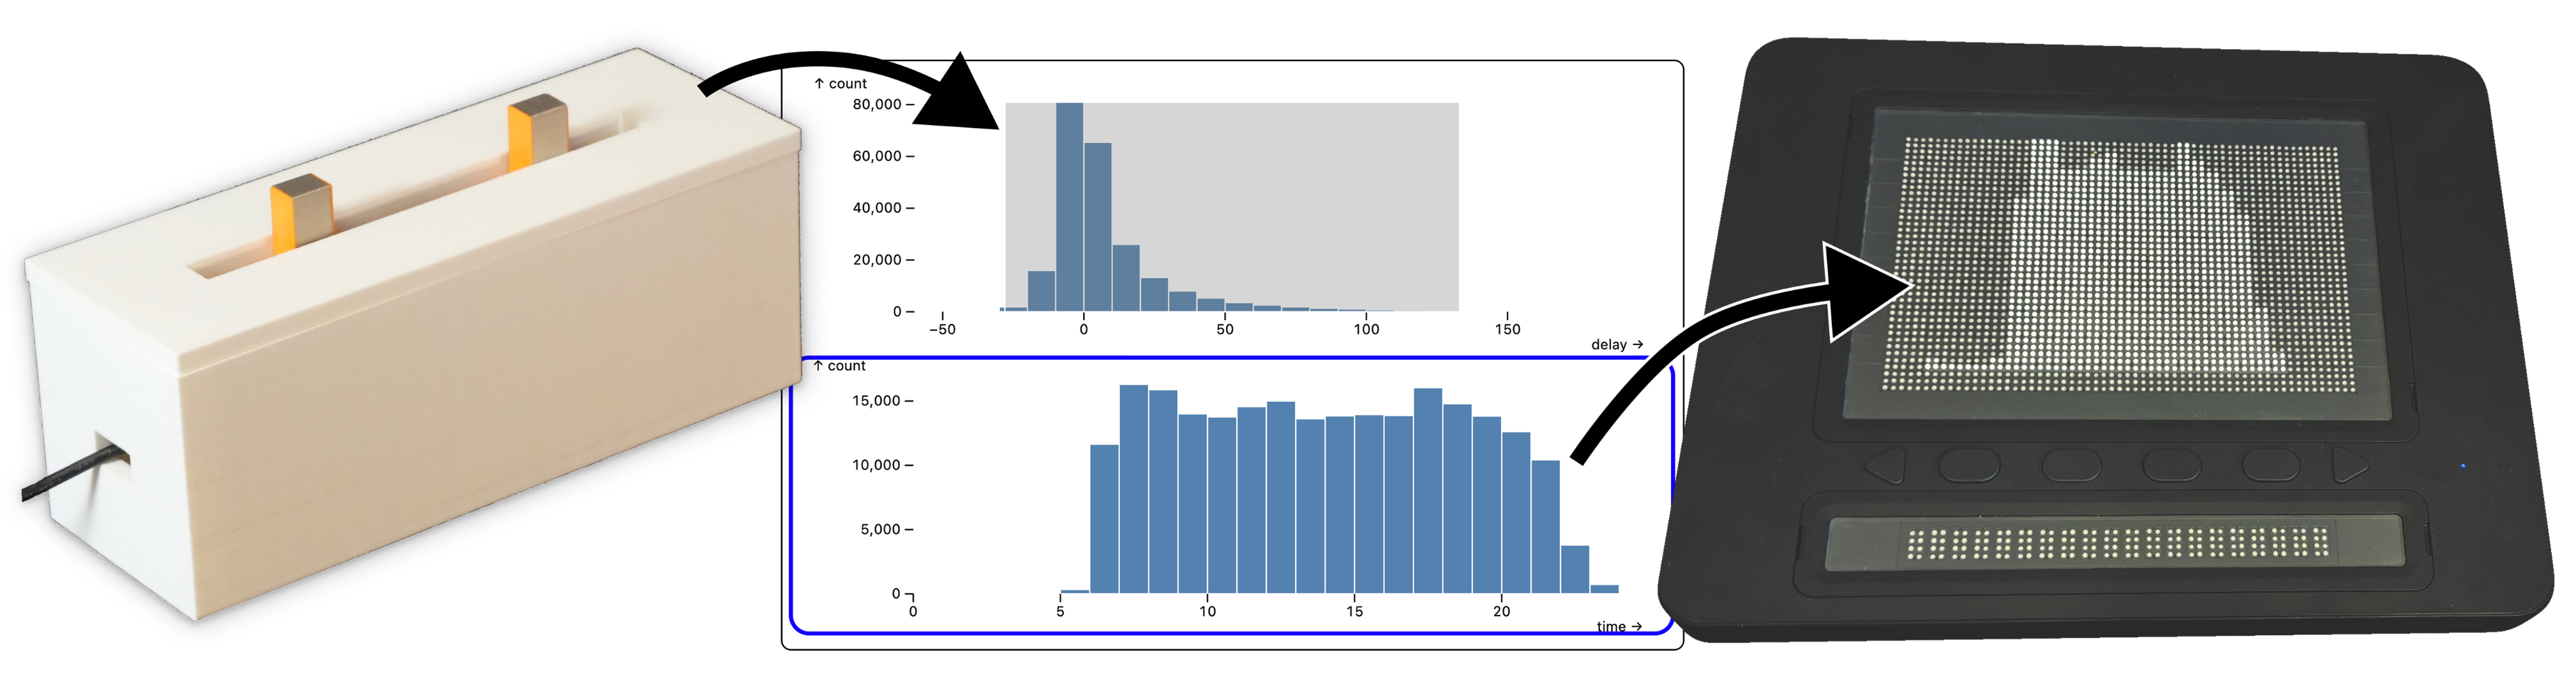
\includegraphics[width=\linewidth, alt={A schematic of a device with a rail and two handles. This device manipulates a chart and a separate chart is rendered as a tactile graph on a refreshable braille display.}]{hero}
  \caption{%
  	Interaction and perception in one space while being able to perceive output in a separate space is the cornerstone of cross-filtering. Our prototype \textit{cross-feelter} (left) can manipulate a visual cross-filter on one visualization (middle) in order to produce output in a separate visualization, as a tactile graphic (right).%
  }
  \label{fig:hero}
\end{figure}
The visualization community has spent decades formalizing interaction techniques for sighted users: brushing scatterplots~\cite{Becker1987}, linking coordinated views~\cite{buja1991interactive}, and cross-filtering aggregated data to rapidly surface relationships across dimensions~\cite{ahlberg1994visual, Weaver2008}. These techniques are not only conveniences. Empirical work has shown that fast, direct manipulation of data fundamentally changes the speed and character of hypothesis generation, and that even small increases in interaction latency measurably reduce the quality of exploratory analysis~\cite{Liu2014, Fisher2012}.

Accessible visualization research has made substantial and genuine progress in recent years. Blind users can access data through rich text descriptions~\cite{Lundgard2022Accessible, Jung2022Communicating}, sonification~\cite{Kim2024, Holloway2022, Zong2024}, and tactile representations~\cite{Marriott, sun2025tactile, Butler2021Technology, Holloway2024, Marriott2026, Smiley2025}. Increasingly, this work extends beyond rendering to \textit{interaction}: screen readers support structured traversal of chart elements and their relationships at varying levels of granularity~\cite{Zong2022Rich,Elavsky2023,Mei2025}, and multimodal systems pair conversational agents with tactile displays to support rich data exploration~\cite{Reinders2025}.

What existing work addresses is, broadly, the question: \textit{what is here?} A blind user can navigate a data representation to understand its structure, locate specific values, extract summary statistics, ask descriptive questions, and build a mental model of what the data contains. This is \textit{access-oriented} interaction, and current tools support it with increasing sophistication.

What remains largely absent from accessible visualization is a different kind of interaction entirely: the \textit{analysis-oriented} kind, in which a user not only reads a dataset but actively operates on it: filtering subsets, conjecturing relationships, testing hypotheses, and generating new knowledge through iterative manipulation. These are the fundamental activities of interactive data science, and they have a different character from access-oriented interaction. Questions shift from ``\textit{what is here?}'' to ``\textit{what happens to Y when I constrain X?}'' According to taxonomies of analytical tasks, existing work has largely not addressed ``characterizing distributions'' and ``correlating'' tasks, which are fundamental to hypothesis-construction~\cite{Amar2005}.

We propose \textit{cross-perception}, an interaction technique that adapts cross-filtering for non-visual contexts while preserving the simultaneity that makes it analytically useful. Cross-perception is defined by two properties. First, \textit{coordinated tactile brushing}: the user manipulates a persistent tactile input in one interaction space, selecting a range across a data dimension. Second, \textit{linked perceptual output}: the computational result of that manipulation is immediately perceivable in a separate space, without requiring serial navigation between them. Together, these properties support not only access to data but active analytical engagement with it: the capacity to ask iterative questions through direct manipulation.

To evaluate cross-perception and explore its design space, we built the \textit{cross-feelter}: a prototype device with two motorized linear faders that maintain persistent, absolute tactile position for brush handles, paired with a refreshable braille display for tactile output. We conducted a within-subjects study with 15 blind participants, comparing the cross-feelter against a screen reader baseline on structured and open-ended data exploration tasks.

In our work, we address four research questions:

\newcommand{\goalref}[1]{\hyperref[goal:#1]{#1}}
\newcommand{\rqref}[1]{\hyperref[rq:#1]{#1}}

% \begin{itemize}[itemsep=-0.5pt]
\begin{enumerate}[label=\textbf{R\arabic*}]
    \item \label{rq:R1}\textbf{(Exploratory):} How might we formalize a tactile interaction approach that enables coordinated, non-visual interaction and perception across multiple spaces?
    \item \label{rq:R2}\textbf{(Quantitative: Objective):} In what measurable ways can we observe improvements to blind data interaction using our approach, in terms of speed, accuracy, precision, and quantity of data queries?
    \item \label{rq:R3}\textbf{(Quantitative: Subjective):} What are the self-reported effects on stress, cognitive load, anxiety, and enjoyment when using our approach?
    \item \label{rq:R4}\textbf{(Qualitative):} In what ways do blind data practitioners imagine extending our approach and its instantiating hardware to new contexts?
\end{enumerate}

This paper makes three contributions. First, we formalize \textit{cross-perception} as an interaction technique for non-visual \textit{analytical} data interaction; one that equips blind users to actively filter, conjecture, and test hypotheses through direct tactile manipulation, not only to access and navigate data~(\Cref{sec:technique}). Second, we provide an empirical evaluation demonstrating that cross-perception yields substantial improvements in exploration speed, query generation, and user experience relative to screen reader interaction, while maintaining comparable accuracy and precision~(\Cref{sec:prototype}--\ref{sec:results}). Third, we argue that accessible visualization has made significant progress at the access-oriented tier of interaction, and that our field's frontier has shifted: the work now should be to give blind users \textit{analytical agency}: the ability to interrogate data, not only to read it~(\Cref{sec:discussion}).

\section{Related Work}
\label{sec:relwork}

This paper sits at the intersection of two bodies of work: research on cross-filtering and analytical interaction in data visualization, and research on making data accessible to blind users. We review each in turn, then characterize the specific gap that cross-perception addresses.

\subsection{Cross-Filtering and Interactive Visual Analysis} 

\textbf{A note on terminology.} \textit{Brushing} is the direct manipulation gesture of selecting a contiguous visual range across a data dimension~\cite{Becker1987}. \textit{Linking} propagates that selection across coordinated views~\cite{buja1991interactive}. \textit{Cross-filtering} applies the linked operation as a filter on shared underlying data, constraining what is visible across views rather than merely annotating selections~\cite{ahlberg1994visual, Weaver2008}.

What makes cross-filtering analytically valuable is not that users can manipulate the interface, but that the gesture and its computational consequence are perceived simultaneously. Even 500ms of additional latency measurably reduces the rate at which users generate observations and formulate hypotheses~\cite{Liu2014}, and providing partial results incrementally reduces but does not eliminate this cost~\cite{Fisher2012}. Temporal coupling between input and output is the mechanism by which direct manipulation supports hypothesis generation, not an implementation detail~\cite{Heer2007}. Recent work on scalable cross-filtering has continued to optimize this coupling through improved architectures~\cite{heer_mosaic_2023}, including pre-computed aggregates~\cite{Moritz2019}. This distinction, between analytical interaction that constructs new information through manipulation and navigational interaction that locates information already present, motivates the core design challenge of cross-perception.

Previous work establishes that cross-filtering supports \textit{analytical} interaction, in which the user constructs and tests hypotheses through rapid, iterative, direct manipulation, rather than navigating toward information that is already present. The value of this analytical interaction is that the user, not a system, gains new insights, questions, and understanding~\cite{Shneiderman1992}.


\subsection{Non-Visual Data Representations} 

Accessible visualization has produced many systems for making data perceivable to blind users across text, audio, and tactile modalities~\cite{Lundgard2022Accessible, Jung2022Communicating, Kim2024, Engel2017, Race2023, sun2025tactile, Gorlewicz2020}. We position cross-perception as complementing this work: many rendering and representation problems have made significant advancements in recent years; but analytical interaction problems, comparatively, have not. 

\textbf{Sonification.} Sonification, mapping data variables to auditory properties such as pitch or timbre, is a distinct and sophisticated field with its own tooling, theory, and evaluation methodologies~\cite{Hermann2011}. Recent work has formalized sonification as a first-class rendering approach with grammar-level expressiveness, enabling mappings comparable in richness to visual encodings~\cite{Kim2024}. Some work has explored data-centric approaches that treat sonification and visualization as parallel co-equal representations~\cite{Zong2024}.

A note on auditory perception is warranted: the human auditory system is capable of parsing concurrent streams and segregating them into distinct perceptual objects~\cite{bregman1990auditory}. However, the relevant constraint for blind and low vision users working with data is more specific: in task-driven contexts, synthesized speech from a screen reader competes with data-representing audio in the same channel, increasing cognitive load of the user and providing complex challenges for authors when designing speech audio and sonification interfaces~\cite{Gherri2011, Kim2024, Thompson2023Chart}. Dual-task and multi-task operations become difficult or impossible, which is a design challenge for cross-filtering specifically, where the filter state and its output must be perceived simultaneously.

\textbf{Tactile and haptic output.} Research on tactile data representation spans several decades, from foundational work on tactual perception~\cite{Schiff1983} to recent studies formalizing tactile alternatives to common chart types~\cite{Engel2017, Race2023}. More recent work has explored simultaneous tactile-and-audio output~\cite{Butler2021Technology}, slide-tone and tilt-tone haptic encodings for shape characteristics of graphs~\cite{Fan2022}, comparative studies on tactile vs audio output~\cite{Chundury2026}, and design guidelines for multimodal touchscreen-based graphics that inform both resolution and tactile landmark placement~\cite{Gorlewicz2020}.

\subsection{Access-Oriented Data Interaction} 

In parallel with rendering advances, accessible visualization has developed increasingly sophisticated interaction techniques for blind users, such as serial and multi-directional navigation across data structures using a screen reader~\cite{Zong2022Rich, Elavsky2023}. However, screen reader traversal is sequential and discrete, which impacts a blind user's ability to extract information from visualizations, impacting accuracy by 61\% and costing 210\% more time doing so~\cite{Sharif2021}. Empirical work has engaged ``questions'' that everyday blind folks have of data representations~\cite{Kim2023Exploring}, and most recently, conversational agents have been paired with refreshable tactile displays to support question-based exploration combining voice input with tactile output~\cite{Reinders2025}.

These systems share a common character: they support \textit{access-oriented interaction}, attempting to bridge the gaps that exist between sighted and blind access to information. However, the activities that remains unsupported requires constructing information through manipulation rather than locating it through navigation; the work of professional data science. In analysis-oriented interaction, the question is not merely lookup or query tasks such as \textit{what is the value at this position} but along the lines of \textit{what is the joint distribution within this subrange}, an answer that does not exist until a filter is applied (and a question that may not even exist unless within a system that supports direct interaction and iteration with the data).

\subsection{Tactile and Haptic \textit{Input}} 

% The reviewers of our CHI submission noted that we understated the breadth of existing tactile and haptic interaction research.... I havne't really expanded on this from the previous draft.

Tactile and haptic input for data interaction has been explored in immersive contexts (not related to accessibility or blind interaction). For example, Cordeil and colleagues' \textit{embodied axes} allow manipulation of data axes as physical objects in augmented reality~\cite{Cordeil2020}, and the \textit{MADE-Axis} extends this to motorized dual-axis faders for AR/VR data environments, demonstrating a cross-filtering use case~\cite{Smiley2021}. Both leverage tactile input and motorized output, though both presuppose sighted users in visual contexts.

Within accessibility-specific work, a touchpad-based brush interface showed 1D filter selection feasibility but provides no queryable positional state when the user's hand is lifted~\cite{Sharif2024}. And a non-motorized slider within an accessible smartphone interface shows the principle of persistent tactile state~\cite{Zhang2018} but cannot be programmatically positioned, which cross-filtering requires for two-way synchronization.

The gap that remains is specific: persistent physical state and simultaneity of input and output perception are both necessary for analytical interaction, and no existing accessible system combines them.

Cross-perception is our attempt to address this gap. Our design is informed by the principles reviewed above: the temporal coupling of cross-filtering, the persistent-state affordances of motorized tactile input, and the insights from prior work on non-visual data interaction regarding the importance of simultaneity, spatial memory, and multi-channel perception. The following section formalizes these into a set of design goals for the interaction technique.

\section{Formalizing Cross-Perception}
\label{sec:technique}

Cross-perception is a tactile interaction technique defined by two properties. First, \textit{coordinated tactile brushing}: the user manipulates a persistent tactile input in one interaction space, selecting a range across a data dimension. Second, \textit{linked perceptual output}: the computational result of that manipulation is immediately perceivable in a separate space, without requiring serial navigation between them. These properties directly instantiate the simultaneity requirement established in \Cref{sec:relwork}: brush state and its consequence are perceived together, in the same moment, supporting the rapid inference cycles of analysis-oriented interaction.

In this section, we formalize cross-perception by deriving six design goals from the principles reviewed in the related work. We begin with a design vignette with our co-designer and co-author [REDACTED], that illustrates how the same cognitive mechanisms that underpin our goals appear in naturalistic blind interaction with physical documents.

% NOTE: "Formalizing" here means: stating, as explicit design % requirements, the principles established in Related Work. % G1-G6 are not intuitions; each has a citation chain in §2. % Make that chain visible in the goal statements below.


\subsection{A Design Vignette: Fuzzy Search and Dual-Task Comparison in Naturalistic Blind Reading} 
\label{sec:vignette}

The following vignette, shared with permission by our blind co-designer and co-author [REDACTED], illustrates two tactile interaction strategies that correspond directly to our design requirements formalized below. We present this vignette as both grounded in the cognitive science and visualization literature reviewed in \Cref{sec:relwork} as well as evidence that the principles we derive from that literature describe real, expert-level behavior in the wild.

[REDACTED], a blind neuroscience engineer, was reading an embossed academic paper and explaining a particular equation to the primary author as the equation recurred and evolved across multiple pages. The embossed format provides high-resolution tactile rendering at up to 100 dots per inch, and [REDACTED] interacted with it using two strategies we have named \textit{fuzzy tactile search} and \textit{dual-task comparison}.

\textit{Fuzzy tactile search} is a spatial indexing strategy. [REDACTED] picked up the stack of pages and thumbed to an approximate location based on tactile position in the stack, touched near the top of the page, immediately recognized from the local texture pattern that he was one page off, flipped to the next page, and navigated directly to the spatial region where the equation began. He then repeated this process to locate the equation's recurrence later in the paper. The strategy relies on two cognitive functions reviewed in \Cref{sec:relwork}: spatial memory, encoding the approximate location of content within a document's physical structure,~\cite{Broadbent2004, Cockburn2002, DellaSala1999} and \textit{object-location memory}, the ability to retain and retrieve the position of objects without continuous visual or tactile contact~\cite{GarciaNavarra2025, Li2011, Llana2025}. Both functions require that objects \textit{have} a stable spatial position to encode: they cannot operate on a system where position is reassigned or meaningless.

\textit{Dual-task comparison} is a simultaneous spatial reasoning strategy. Having located the same equation in two places, [REDACTED] placed one hand on each and skimmed both simultaneously, stopping when his hands detected the point of divergence between them. He explained the evolution of the equation by reference to that divergence. This strategy demonstrates exactly the interaction character that cross-filtering supports for sighted users: two data regions perceived in parallel, with relational structure emerging from simultaneous contact rather than sequential reading. It also demonstrates the additional requirement of \textit{simultaneous multi-location tactile interaction}: a user resting a pinky on a known reference point while exploring relative to it with another finger, a pattern documented in prior empirical work on tactile interactive systems~\cite{Gorlewicz2020}.

Together, these strategies illustrate a key observation: skilled blind readers of physical documents are not limited to sequential access. The constraint is architectural: the medium must maintain a persistent, meaningful spatial state so that object-location memory can operate, and it must allow simultaneous multi-point contact so that comparison can occur. Our design goals operationalize these requirements for computational, analytical interaction with tactile interfaces.


\subsection{Design Goals} 

We derive six design goals from the principles established in \Cref{sec:relwork} and illustrated by the vignette above.

\begin{enumerate}[label=\textbf{G\arabic*:}, leftmargin=0pt, itemindent=!, itemsep=0pt, topsep=0pt, parsep=0pt]

\item \label{goal:G1}\textbf{Maintain and reflect system state through tactile location.} Object-location memory requires objects with stable, queryable positions~\cite{GarciaNavarra2025, Llana2025}. Tactile input elements must therefore have absolute, persistent positional state: the knob must remain where the user or system last placed it and be readable by touch without performing an action. This also enables motorized two-way synchronization, where the system sets knob position as output and the user sets it as input.

\item \label{goal:G2}\textbf{Allow for multiple simultaneous channels of perception.} Synthesized speech competes with data-representing audio under cognitive load~\cite{Gherri2011}. Cross-perception routes data manipulation to a tactile input channel, eliminating this competition. Audio output via ARIA-live announcements remains available for precise positional feedback but is kept serial and non-competing.

\item \label{goal:G3}\textbf{Correspond tactile-to-computational functional semantics.} Interface elements should have names and behaviors that describe what they do~\cite{WAI2008, Elavsky2022Chartability}. The visual cross-filtering metaphor involves dragging handles along a spatial dimension; cross-perception preserves this by mapping a physical rail sliding to setting a filter boundary, reducing translation between user action and analytical action.

\item \label{goal:G4}\textbf{Provide linked interaction across multiple data dimensions.} Cross-filtering requires that a filter on one dimension immediately propagates to constrain coordinated views of others that share the same underlying dataset~\cite{buja1991interactive, ahlberg1994visual}. The filter state set by tactile input must immediately determine the output displayed in linked views; without this, the technique only accomplishes single-view selection.

\item \label{goal:G5}\textbf{Support fast, dynamic, and reversible interaction.} The analytical value of cross-filtering depends on rapid hypothesis iteration~\cite{Liu2014, Fisher2012}. Filter adjustments must be continuous and incremental, system response must be low-latency, and any state must be immediately reversible. These motivate motorized faders with 1024 units of precision and a pre-computed data cube backend~\cite{heer_mosaic_2023}.

\item \label{goal:G6}\textbf{Facilitate user-driven exploration.} Cross-filtering is a direct manipulation paradigm in which the user, not an algorithm, controls the analytical flow~\cite{ahlberg1994visual, Shneiderman1992}. The user's physical manipulation of the filter handles is the direct and sole determinant of what the tactile output displays, with no intermediary statistical, language model, or non-deterministic interpretation.

\end{enumerate}

\section{Prototype: The Cross-Feelter}
\label{sec:prototype}

\begin{figure}[h]% specify a combination of t, b, p, or h for top, bottom, on its own page, or here
  \centering % avoid the use of \begin{center}...\end{center} and use \centering instead (more compact)
  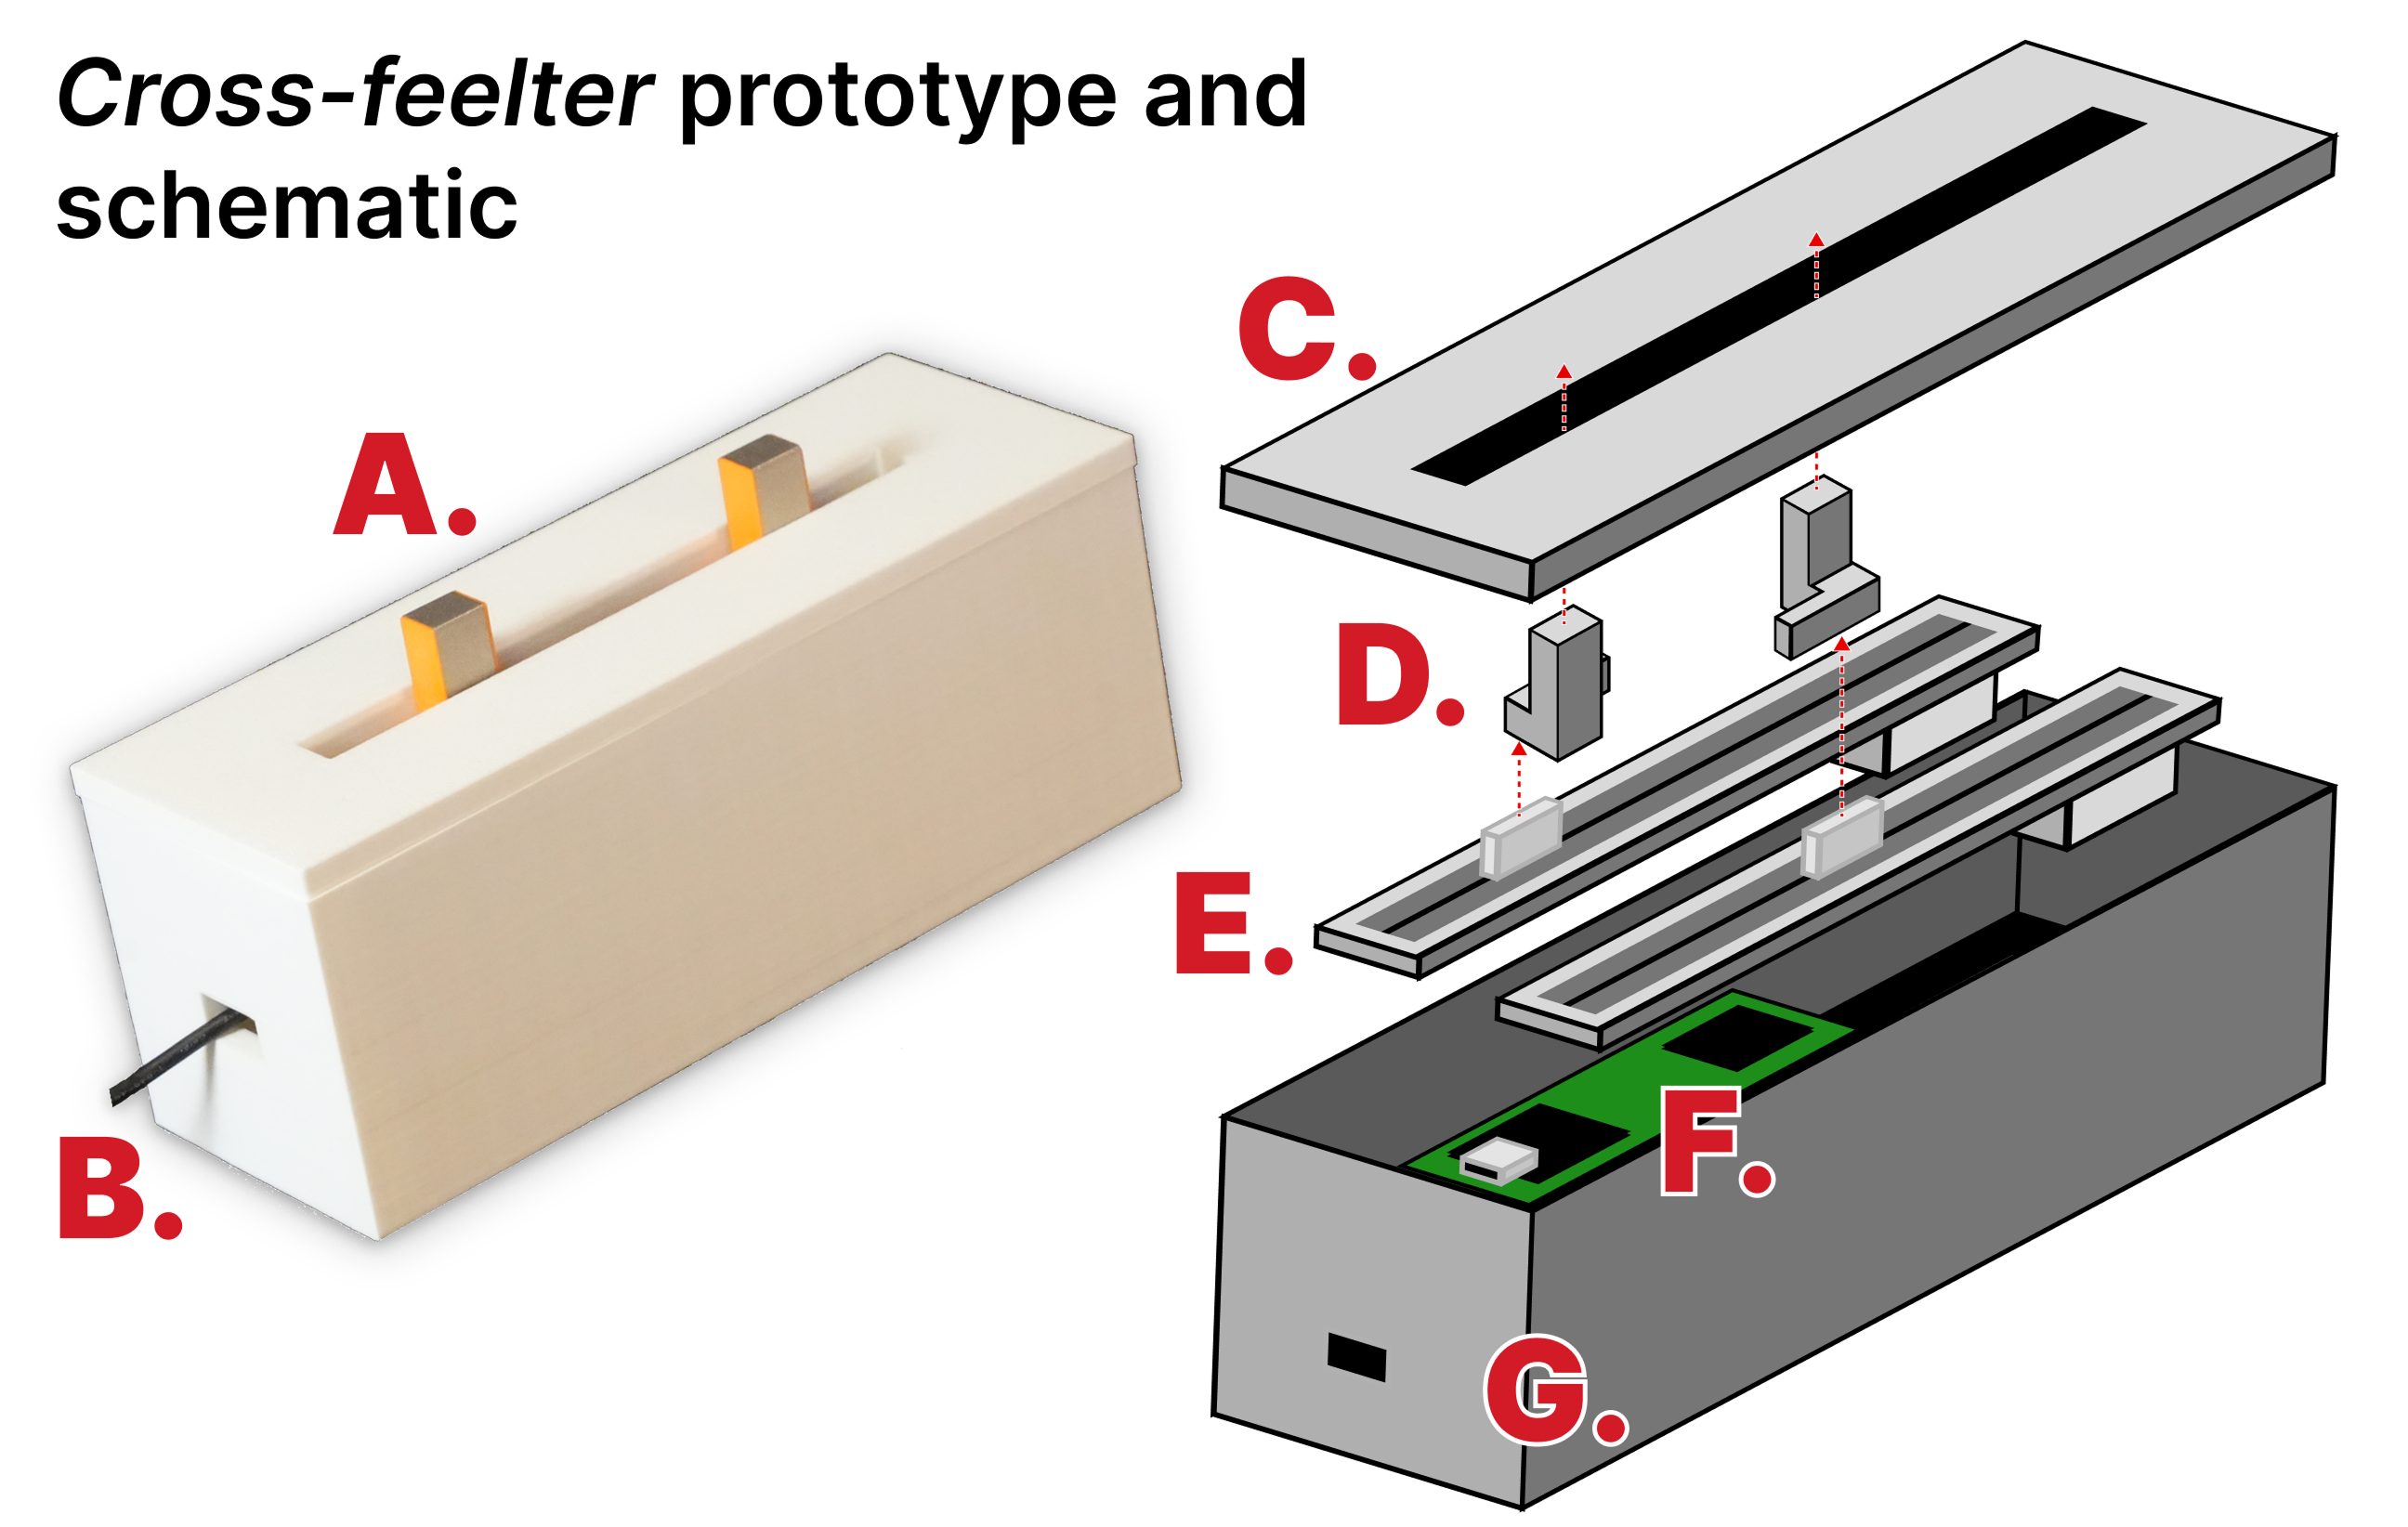
\includegraphics[width=\columnwidth, alt={Our prototype with a blown up version where all the parts are shown separately.}]{figures/proto.png}
  \caption{%
  	A. Our prototype \textit{cross-feelter}. B. USB output (to computer). C. 3D printed rail cover. D. 3D printed knobs that consolidate rails into one. E. 2 motorized linear potentiometers. F. Arduino board. G. 3D printed casing.%
  }
  \label{fig:proto}
\end{figure}

\noindent We instantiate cross-perception in a hardware prototype we call the \textit{cross-feelter}: a device with two motorized linear faders that provide persistent, absolute tactile input state for brush handles, paired with a refreshable braille display for coordinated tactile output. All hardware schematics, firmware, and interface code are open-sourced at \url{[REDACTED]}; 3D-printable STL files for the housing components are available in our supplemental materials and on Thingiverse at \url{[REDACTED]}. The total cost of hardware components is \$30--50 USD, which we designed intentionally to enable replication by the DIY-AT and maker communities~\cite{Hurst2011,Smiley2025}.


\subsection{Interaction Flow} 

We begin with an idealized walkthrough of what a blind analyst actually does when using the cross-feelter to perform a cross-filtering task. This is the ground truth from which the hardware design choices derive; we describe the hardware in \Cref{sec:hardware} with reference to the steps below.

Consider an analyst exploring a dataset of local rent prices and transit access across city neighborhoods. Three linked histograms are rendered in sequence on the refreshable braille display. The analyst wants to ask: \textit{do neighborhoods with the highest rents also have better transit access?} At startup, the left knob sits at 0\% and the right at 100\%, representing an unfiltered view of the full distribution.

\textbf{Step 1: Feel and filter.} The analyst feels the starting state of the tactile data representations on the refreshable braille display, navigating between each chart and hearing supplemental screen reader descriptions alongside the touchable shapes formed from the pins. The analyst moves their hand or hands to the feelter device and slides the left knob rightward, narrowing the filter from below. As they move, an ARIA-live announcement reports the current percentage and knob name via the screen reader, providing precise serial feedback for positioning (\goalref{G2}). The analyst moves the right knob slightly leftward, hearing another announcement. The two knobs now define a range, say 75\% to 90\% of the rent distribution.

\textbf{Step 2: Perceive the consequence.} During filtering, the analytical environment updates linked histograms immediately on each knob movement. The analyst navigates the braille display to the transit histogram without touching the knobs. Because the knobs are motorized and maintain position, the filter state is preserved and readable by touch at any time (\goalref{G1}). They feel the updated distribution and compare it to the shape they perceived in the unfiltered state.

\textbf{Step 3: Iterate.} The analyst slides the left knob further right, narrowing to the top 10\% of rents. The display updates. They feel the new shape. The pattern sharpens or changes, and they iterate again, building toward a hypothesis in the same cycle that sighted analysts perform visually. Each knob adjustment is a computational query: a gesture that constructs a question and immediately exposes its answer.

\subsection{Hardware Design} \label{sec:hardware} 

The cross-feelter uses two motorized linear potentiometers (commonly called motorized faders in sound design hardware) mounted side by side in a 3D-printed housing (see \Cref{fig:proto}). Each fader provides a physical knob on a bounded rail.

\textbf{Motorized, absolute-position faders (\goalref{G1}, \goalref{G5}).} We chose rail-based faders over alternatives (touchpad, rotary encoder, joystick) for two reasons grounded in the \goalref{G1} requirement. First, the fader is \textit{absolute}: the knob's physical position on the rail directly corresponds to the filter boundary value, with no drift or accumulation. Second, the fader is \textit{motorized}: the system can programmatically set knob position as well as read it. This bidirectionality is essential for cross-filtering: the system must be able to reset filter state on condition changes, counterbalance, and initialization, not only receive input. Prior work on brush-based accessible interfaces~\cite{Sharif2024} used a touchpad, which provides no queryable positional state when the hand is lifted; prior work using non-motorized sliders~\cite{Zhang2018} cannot be programmatically positioned. The motorized fader solves both problems.

Each rail terminates in a tactile boundary, a strong edge inset 4mm from the housing wall per tactile design guidelines~\cite{Gorlewicz2020}, so the analyst can feel both the knob position \textit{and} its position relative to each end of the scale (\goalref{G1}). The API reads and writes fader position every 5ms, providing up to 1024 units of precision, which maps well to histogram bin resolutions in practical cross-filtering datasets (\goalref{G6}).

\textbf{Merged-rail housing (\goalref{G3}).} We designed two housing configurations: one exposing the rails independently, and one using angled knobs to place both rails along a single track (\Cref{fig:proto}, part D). The merged-rail design, used for all data tasks in the study, ensures the left knob remains to the left of the right knob at all times (they cannot cross over). This preserves the functional semantics of a spatial filter range: left boundary is always left, right boundary is always right, matching the computational filter and the visual histogram (\goalref{G3}). The independent-rail configuration was used for the video interaction training task (\Cref{sec:videotraining}), where the two rails served different functions (volume and position).

Our dual-fader design is similar in form to motorized fader-based systems proposed for axis interaction in AR/VR data environments~\cite{Smiley2021, Cordeil2020}; however, those systems presuppose sighted users operating in 3D visual contexts. Our design differs in three ways: (a) the housing constrains the two faders to a single interaction dimension to support filter semantics; (b) the motorized positioning enables two-way synchronization with the data interface; and (c) the entire system is designed for eyes-free operation as the primary use mode.

\textbf{ARIA-live auditory feedback (\goalref{G2}).} When a knob is moved, the interface emits an ARIA-live announcement to the screen reader reporting the new filter percentage. ARIA-live is set to \texttt{polite} mode, meaning announcements queue behind any active screen reader speech rather than interrupting it. This provides precise, serial auditory feedback for filter positioning without competing with other auditory streams in the environment (\goalref{G2}). Tactile feedback (the knob's physical position) and auditory feedback (the ARIA announcement) thus serve complementary roles: tactile provides continuous, queryable approximate state; auditory provides precise on-demand readout triggered by movement.


\subsection{Analytical Environment} \label{sec:environment} 

\begin{figure}[h]% specify a combination of t, b, p, or h for top, bottom, on its own page, or here
  \centering % avoid the use of \begin{center}...\end{center} and use \centering instead (more compact)
  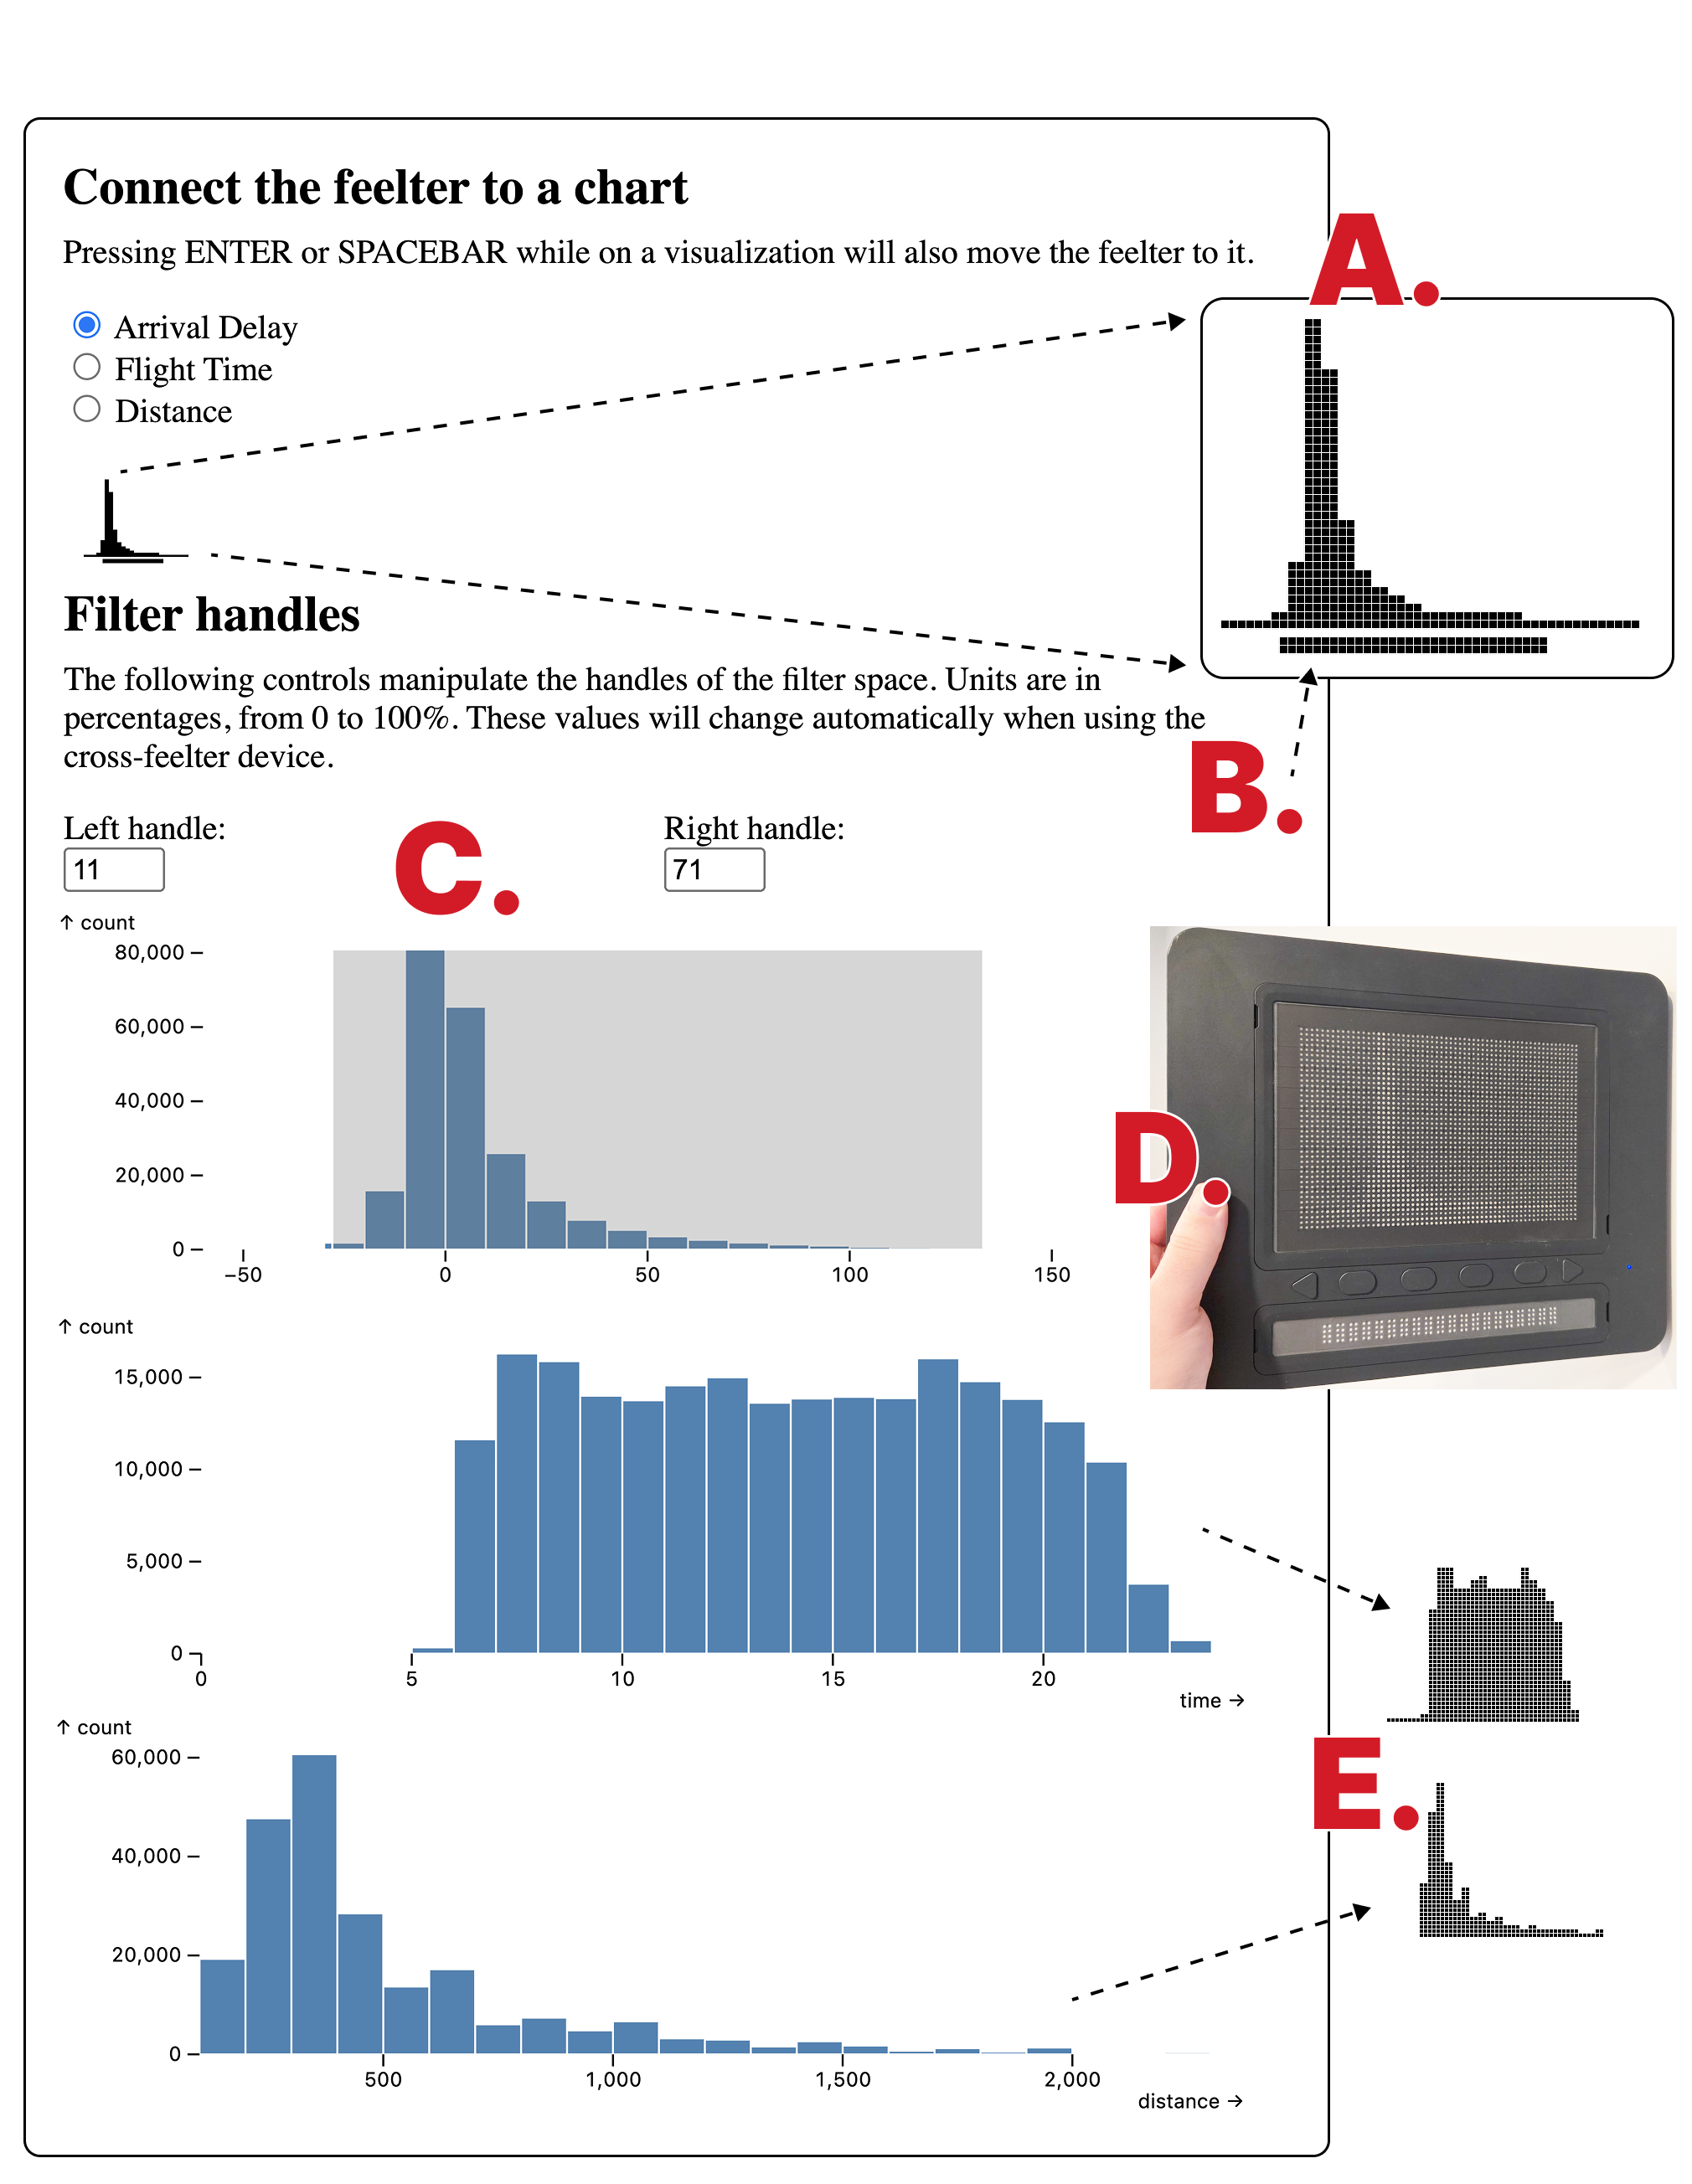
\includegraphics[width=0.5\columnwidth, alt={Our analytical environment with 3 visualizations as well as instructions for connecting devices and controlling the filter.}]{figures/analysis.png}
  \caption{%
  	Our analytical environment. A. a 1 to 1 translation between visual and tactile that represents a 60x40 pixel-to-pin array. B. A tactile version of the filter location (if on the chart being focused). C. Cross-filtering controls, including text inputs for screen-reader only manipulation. D. Refreshable tactile display output. E. Example renderings of the other 2 charts.%
  }
  \label{fig:analytical}
\end{figure}

The cross-feelter operates within a web-based analytical environment purpose-built for this study (\Cref{fig:analytical}). The environment presents three linked histograms derived from different variables in a shared dataset. Each histogram is rendered both visually (for debugging and sighted collaborators) and as a 60$\times$40 pin array sent to the Dot Pad refreshable braille display.

\textbf{Cross-filtering backend (\goalref{G4}, \goalref{G5}).} We use Mosaic~\cite{heer_mosaic_2023} to manage the cross-filtering logic. Mosaic pre-aggregates filter results across binned input values, enabling fast, low-latency responses to filter changes even over larger datasets (\goalref{G5}). It also provides a straightforward API for specifying a brush-filter interaction layer over a histogram dimension, including programmatic control of filter state and undo actions (\goalref{G5}). When the user moves a fader knob, the new filter boundaries are sent to Mosaic, which immediately updates the linked histograms, which are then re-rendered on the braille display. The render cycle from fader movement to updated tactile output is 500--1200ms on the Dot Pad hardware, fast enough to support iterative exploration, though slower than visual cross-filtering systems and a recognized limitation (\Cref{sec:limitations}).

\textbf{Braille display output (\goalref{G2}).} The Dot Pad provides a 60$\times$40 binary pin array (pins raise or lower on command). We render each histogram as a bitmap at this resolution, trading fidelity for speed relative to a high-resolution braille embosser (which takes 3--4 minutes per page). At any time, the braille display shows one chart; the analyst navigates between charts using the screen reader. The visual representation of the target pin array is visible to sighted observers and collaborators in the environment (\Cref{fig:analytical}, part A), illustrating the resolution gap that future advances in refreshable display technology could close.

\textbf{Screen reader compatibility.} The analytical environment is a standard web interface, accessible via any JAWS, NVDA, or VoiceOver-compatible screen reader. Cross-filter input controls are exposed as labeled range inputs so they can be operated by screen reader alone (providing the baseline condition for our study, \Cref{sec:study}). The ARIA-live region for fader announcements is separate from these controls and does not interfere with standard screen reader navigation of the interface.

% Our evaluation engages two of our research questions:

% \begin{enumerate}
%     \item [\textbf{R2}] (Quantitative: Objective) In what measurable ways can we observe potential improvements to blind data interaction using our tactile interaction approach?
%     \item [\textbf{R3}] (Quantitative: Subjective) What are the self-reported benefits, opportunities, and challenges that blind people experience when using our tactile interaction approach?
% \end{enumerate}

% \subsection{Participants}
% We conducted our study with 15 total participants, 8 who did not have existing professional expertise working with data and 7 who did. 7 of our participants identified as male, 8 as female.  

% All 8 of our participants without existing data expertise, in addition to 2 of our participants with existing data expertise, were recruited locally through existing relationships and social networks. We reached out to local participants via email and in-person at community events. 

% For our remaining 5 participants with data expertise, we coordinated our studies to be conducted in person at mutual conferences. We found it difficult to recruit blind data scientists, analysts, and engineers locally; however, we have a wider network of connections outside of our local area. We took advantage of travel and reached out to our remaining participants via email and in person.

% Participants were screened with a short survey for eligibility: we recruited only participants who identified as blind, had screen reader expertise, were 18 or older, and US citizens or permanent residents. The chosen participants were informed of the risks associated with our study, notified in advance that they would be compensated with a \$50 gift card for participation, and that consent to participate is voluntary.

% \subsection{Data-preferences workshop}
% We held 2 preliminary study sessions to test our methodology, polish our process, and find bugs before running the study in full.

% However, we noticed that our preliminary participants were not particularly interested in the data we were using, so we then held a community workshop at our local library of accessible media (a braille and talking book library that services our state). In attendance were 21 members of the community and we discussed which possible datasets they would be most excited to interact with.

% We broke into small groups and discussed things from local to state politics, economics, sports teams, weather, climate, barber shops, rent prices, and more. At the end, members voted on which datasets were most interesting to them and they enthusiastically chose rent prices across the city by neighborhood and ``fish fry locations'' across the city, also organized by neighborhood. Both of these were among the highest voted datasets that are readily available. For context, on what a ``fish fry'' is: our city has a tradition of frying fish during the Catholic lent, during which local businesses and even non-Catholic groups participate. There is a well-curated dataset made available every year.

% https://data.wprdc.org/dataset/pittsburgh-fish-fry-map
% \subsubsection{Blind data novices}
% 8
% \subsubsection{Blind data experts}
% 7
% \subsection{Design}
% 90 min, compensated 

\section{Data Exploration Study} \label{sec:study}

We conducted a within-subjects study comparing cross-feelter-based cross-filtering (CF condition) against screen-reader-based cross-filtering (SR condition) across structured and open-ended data exploration tasks. Sessions were 90 minutes, conducted in person, and approved by our IRB.

 
\subsection{Study Design} 

\textbf{Overview.} Our study employed a 2$\times$2 Latin square design, fully counterbalanced across two factors: (1) condition order (CF-first vs.\ SR-first) and (2) dataset order (flight data vs.\ neighborhood data), producing four participant groups (\Cref{tab:design}).

\begin{table}[h]
\centering
\caption{2$\times$2 Latin square study design. CF = cross-feelter condition; SR = screen reader condition.}
\label{tab:design}
\begin{tabular}{@{}lll@{}}
\toprule
\textbf{Group} & \textbf{Condition order} & \textbf{Dataset order} \\
\midrule
A (n=4) & CF $\rightarrow$ SR & Flight $\rightarrow$ Neighborhood \\
B (n=4) & SR $\rightarrow$ CF & Flight $\rightarrow$ Neighborhood \\
C (n=4) & CF $\rightarrow$ SR & Neighborhood $\rightarrow$ Flight \\
D (n=3) & SR $\rightarrow$ CF & Neighborhood $\rightarrow$ Flight \\
\bottomrule
\end{tabular}
\end{table}

Within each condition, participants performed two tasks on the same dataset: a 3-minute structured data-relationship task followed by a 10-minute open-ended data exploration. Counterbalancing both orders controlled for dataset familiarity, learning effects, and dataset-specific task difficulty.

\textbf{Conditions.} In the \textbf{CF condition}, participants used the cross-feelter (merged-rail housing; \Cref{sec:hardware}) to manipulate cross-filter bounds, with the Dot Pad displaying linked histograms. In the \textbf{SR condition}, participants used their screen reader to operate labeled text input fields exposing the same filter controls, with the same Dot Pad display. The analytical environment was identical across conditions; only the input method differed.

\textbf{Session procedure.} Each session followed this order regardless of group: 
\begin{enumerate}[itemsep=-0.5pt]
  \item Tech setup, baseline interview, introduction to tactile histograms and cross-filtering, baseline anxiety Likert question \textit{(20 min)}
  \item Device familiarization: video interaction task and brief semi-structured interview \textit{(15 min)}
  \item First data condition: structured task, open-ended exploration, Likert-scale interview \textit{(20 min)}
  \item Second data condition: structured task, open-ended exploration, Likert-scale interview \textit{(20 min)}
  \item Closing semi-structured interview \textit{(15 min)}
\end{enumerate}

 
\subsection{Participants} 

We conducted our study with 15 blind participants: 8 without prior professional data expertise and 7 with it (data analysts, scientists, or engineers currently or recently employed in data-related roles). 7~participants identified as male, 8 as female.

Participants without data expertise, plus 2 with it, were recruited locally through community outreach. The remaining 5 participants with data expertise were recruited through professional networks and coordinated at mutual academic conferences, due to difficulty recruiting blind data scientists locally. All participants were screened for eligibility (blind, screen reader proficient, 18 or older, US citizen or permanent resident), informed of risks and voluntary participation, and compensated with a \$50 gift card.

 
\subsection{Datasets} 

Study tasks used two datasets selected through a community data-preference workshop. Pilot sessions revealed that participants were not engaged by our initial generic dataset, so we held a workshop at a local braille and talking book library (n=21 community members). Participants voted on datasets from topics including local politics, housing, and community life. The two highest-voted were: (1) rent prices across city neighborhoods, and (2) fish fry locations across city neighborhoods (a dataset reflecting a regional Catholic Lent food tradition observed broadly across denominations). Both are publicly available. A generic flight dataset was included as the second counterbalanced dataset.

Each dataset was configured with three histogram variables from a shared source, with cross-filter tasks designed to target a 75\%--100\% filter range producing a clear, unambiguous relationship between variables.

 
\subsection{Device Familiarization: Video Interaction Task} 
\label{sec:videotraining}

\textbf{Rationale.} Before data tasks, participants completed a device familiarization activity using the cross-feelter to control a video feed rather than a data chart.

The goal was to build fluency with the motorized fader mechanism (absolute-position input, motorized output, the relationship between physical knob position and system state) without pre-exposing participants to the cross-filtering metaphor, data tasks, or the study datasets. A practice task using data histograms would have constituted condition-specific training, introducing learning effects that could confound the within-subjects comparison. Video scrubbing and volume control are familiar and intuitive interaction goals for all of our users, which served as a way for all of them to understand how to operate the device.

% We used the independent-rail configuration (rather than the merged-rail casing used for data tasks) to demonstrate the device in a different mapping (top rail for volume, bottom rail for playback position) before constraining it to filter-range semantics. This also provided a natural basis for the brief follow-up interview about participants' prior experience navigating video with a screen reader.

\textbf{Task.}
% The top rail controlled volume (tap to play/pause); the bottom rail tracked and controlled playback position. 
Participants were asked to find the name of the person in the video recording, announced early in the clip. This simple information-retrieval goal required genuine device use while keeping cognitive demand low before the main study.

 
\subsection{Introduction to Tactile Histograms and Cross-Filtering} 

At session start, after consent and the baseline interview, we provided a scripted introduction to tactile histograms and cross-filtering. We explained histogram structure, introduced the concept of linked histograms sharing a source dataset, and demonstrated cross-filtering with three histograms from a fruit example dataset, using two sheets of paper held over one histogram to physically simulate a spatial filter.

We framed filtering explicitly as an analytical activity: ``filtering is a way to ask questions more than to find answers, to look for possible relationships that might exist in the data.'' Two follow-up questions gauged comprehension and interest before proceeding.

 
\subsection{Data Tasks} 

\subsubsection{Structured data-relationship task}

Participants cross-filtered the dataset and answered a three-option multiple-choice question within three minutes. The question and options were available via screen reader in the interface; the facilitator restated them only if asked and did not otherwise intervene.

For the flight dataset: \textit{``What is the relationship between filtering for longer flight distances and the arrival time of flights?''} (Correct: longer flights tend to arrive earlier compared to all flights.)

For the neighborhood dataset: \textit{``What is the relationship between filtering for a higher number of fish fry locations and the rent price of a neighborhood?''} (Correct: neighborhoods with more fish fry locations tend to have higher rent prices.)

We measured task completion rate (binary), time to completion (seconds), filter placement precision (distance of handles from target positions of 75\% and 100\%, scored in $\pm$4\% increments awarding 0.5/0.3/0.1 points per handle tier), and answer accuracy (binary).

\subsubsection{Open-ended data exploration}

Participants then performed a 10-minute open-ended exploration of the same dataset using a prompted, concurrent think-aloud method~\cite{Alhadreti2018}. Before beginning, we framed the activity: ``the purpose is not to \textit{answer} questions but to \textit{come up with} questions. This is how many data scientists explore unfamiliar datasets, by looking for possible relationships.''

We measured: (1) \textit{computational queries}: any filter manipulation followed by braille display inspection of one or more linked charts (filter changes without output inspection did not count); and (2) \textit{spoken queries}: any data-related question voiced aloud, regardless of formality or answerability via cross-filtering.

 
\subsection{Measures and Analysis} 

\textbf{Quantitative analysis.} Objective measures (completion rate, time, precision, accuracy, query counts) and subjective measures (5-point Likert scales for stress, cognitive load, future-task anxiety, and enjoyment) were collected per condition. A pre-study baseline anxiety item provided a pre-condition reference.

Analysis was conducted in Python (code and de-identified data in supplemental materials). Objective continuous measures were compared using paired $t$-tests. Likert-scale differences were evaluated using Wilcoxon Signed-Rank tests given the ordinal nature of the data. We report means, standard deviations, test statistics, and $p$-values; group-level results (data experts vs.\ non-experts) are reported separately where they diverge.

\textbf{Qualitative analysis.} Qualitative data comprised session audio/video recordings, facilitator notes, and closing semi-structured interview transcripts. The interview covered three topics: overall experience and condition comparison, interface and environment feedback, and future application ideas.

Analysis proceeded in two stages. In the first stage, two members of the research team independently reviewed all recordings, notes, and transcripts, generating initial codes at the utterance level. Codes captured themes across four domains: device usability (physical interaction, feedback quality, learning curve); condition comparison (speed, cognitive load, perceived control); analytical engagement (question generation, hypothesis articulation, confidence with data); and future use speculation. The two coders then resolved all disagreements through discussion, reaching consensus before proceeding.

In the second stage, codes were organized using affinity diagramming~\cite{Harboe2015}, conducted collaboratively by members of the research team working from the reconciled code set. Resulting themes inform the qualitative findings in \Cref{sec:results} as well as our future use cases in \Cref{sec:futurework}.

\section{Results}
\label{sec:results}

\begin{figure*}[h]% specify a combination of t, b, p, or h for top, bottom, on its own page, or here
  \centering % avoid the use of \begin{center}...\end{center} and use \centering instead (more compact)
  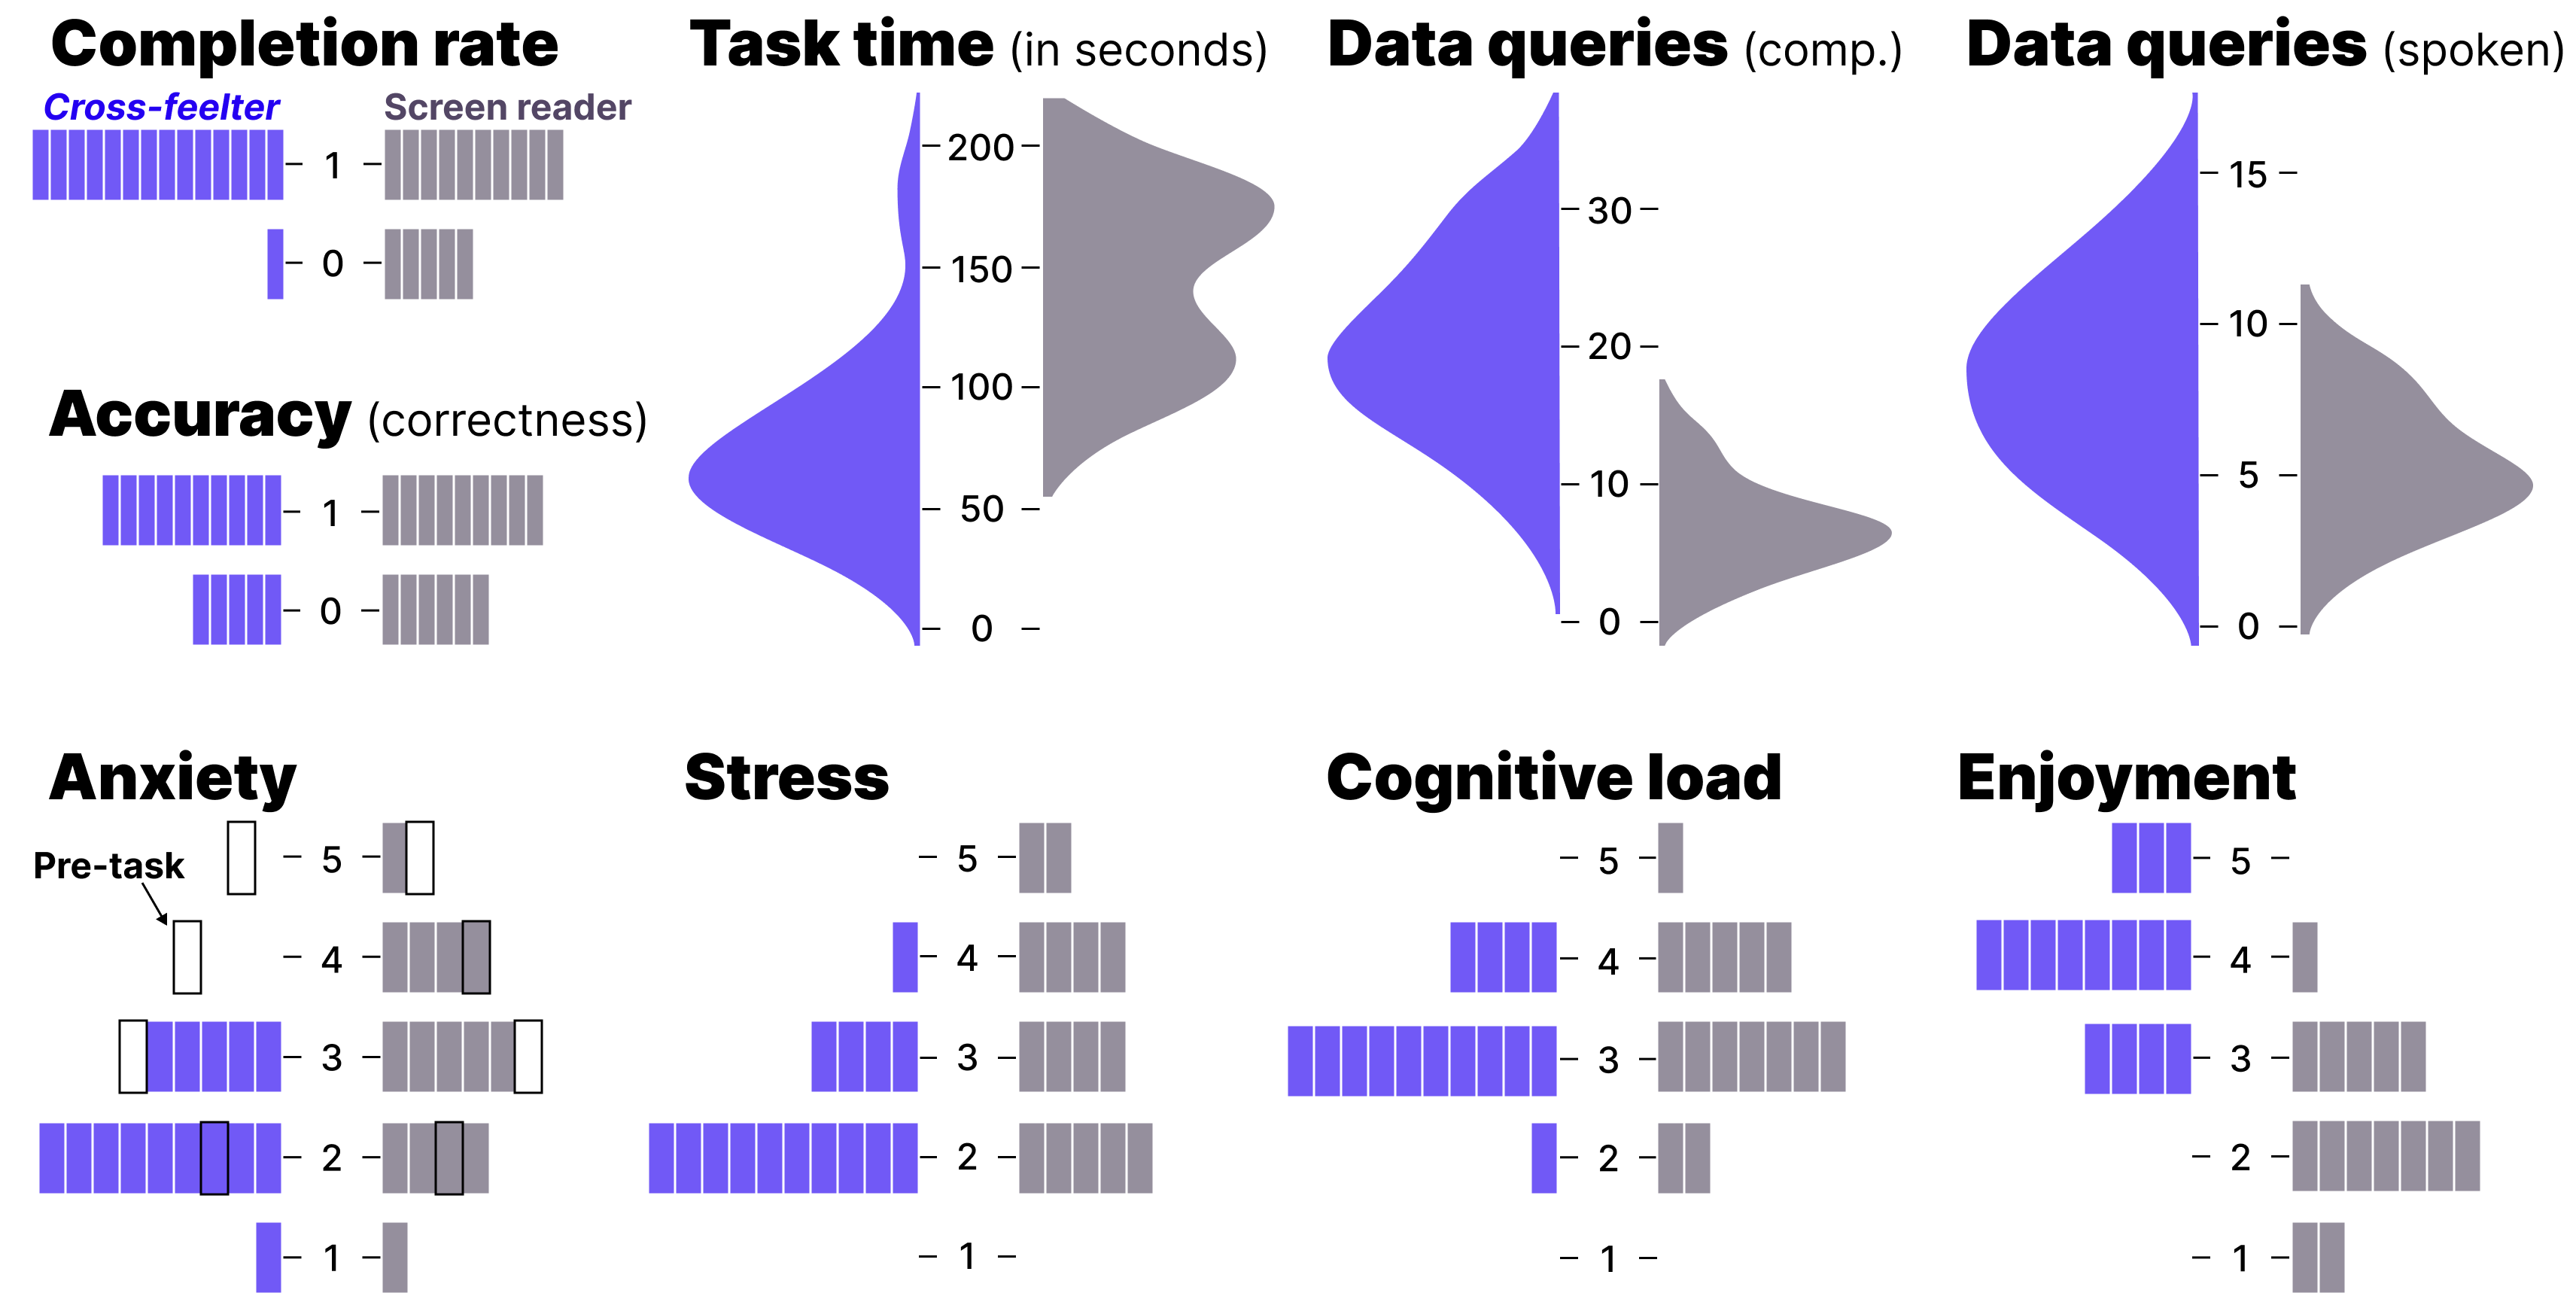
\includegraphics[width=.85\textwidth, alt={9 data visualizations. This short description is inadequate in the space we have, please see our supplemental materials for our data in tabular form, analysis output, and more detailed information.}]{figures/quant.png}
  \caption{%
  	Results. Completion rate and accuracy are counts. Task time, data queries (computational), and data queries (spoken) are objective, observational measures. Anxiety, stress, cognitive load, and enjoyment are Likert-scale results from 1 (``very little'') to 5 (``quite a lot'').%
  }
  \label{fig:quant}
\end{figure*}

Our analysis compared 15 blind participants performing cross-filtering tasks under two conditions: using the cross-feelter (\textbf{CF}) versus using a screen reader alone (\textbf{SR}). We report objective and subjective measures in turn. Full analysis code and de-identified data are available in our supplemental materials. 


\subsection{Objective Results}


\subsubsection{Substantially improved task completion rate and
speed}

For the structured data-relationship task, participants achieved a significantly higher completion rate with CF (mean = 0.93, SD = 0.26) compared to SR (mean = 0.60, SD = 0.51; paired $t$-test: $t = 2.646$, $p = 0.019$). Task completion time was significantly lower in the CF condition (mean = 75.53s, SD = 36.14) than in the SR condition (mean = 143.93s, SD = 34.65; $t = -6.876$, $p < 0.001$), a 90\% improvement in speed.

\subsubsection{Comparable accuracy and precision}

Accuracy (correct multiple-choice answer) was higher in the CF condition (mean = 0.67, SD = 0.49) than SR (mean = 0.53, SD = 0.52), but this difference was not statistically significant ($t = 1.468$, $p = 0.164$). Notably, when filtering for only completed tasks, SR users showed marginally higher accuracy (SR: mean = 0.78; CF: mean = 0.71), though again non-significant ($t = 0.555$, $p = 0.594$). We interpret this in \Cref{sec:discussion-accuracy}.

Filter placement precision (scored by proximity to target handle positions of 75\% and 100\%) was marginally higher in CF (mean = 0.66, SD = 0.37) than SR (mean = 0.59, SD = 0.34), with no significant difference ($t = 0.617$, $p = 0.547$).

\subsubsection{Substantially increased quantity of data queries}

During the open-ended exploration task, CF elicited substantially more computational queries (mean = 20.13, SD = 6.45) than SR (mean = 7.00, SD = 3.18; $t = 9.567$, $p < 0.001$), a 188\% increase. Spoken queries were also significantly higher in CF (mean = 8.20, SD = 3.14) than SR (mean = 5.33, SD = 1.99; $t = 3.765$, $p = 0.002$), a 54\% increase. 


\subsection{Subjective Results}


Subjective measures varied between participants with and without professional data expertise; we report group-level differences where they diverge meaningfully.

\subsubsection{Reduced stress}

Stress ratings were significantly lower in the CF condition (mean = 2.40, median = 2.0) than SR (mean = 3.20, median = 3.0; Wilcoxon $W = 4.000$, $p = 0.013$). The effect was driven primarily by participants without data expertise (CF: mean = 2.62, SR: mean = 3.75; $W = 2.500$, $p = 0.047$). Data experts reported similarly low stress across both conditions (CF: mean = 2.14, SR: mean = 2.57; $W = 0.000$, $p = 0.083$).

\subsubsection{Comparable cognitive load}

Cognitive load showed an observed difference in means (CF: mean = 3.13, SR: mean = 3.47) but was just outside statistical significance ($W = 4.000$, $p = 0.059$). We interpret both conditions as producing comparable cognitive load during task performance.

\subsubsection{Lower future-task anxiety}

Participants in the CF condition reported significantly lower anxiety about performing a future timed data task using the same tools (CF: mean = 2.27, SR: mean = 3.00; $W = 10.000$, $p = 0.017$). CF anxiety was also significantly lower than participants' baseline anxiety measured before any tasks ($W = 5.000$, $p = 0.003$), while SR anxiety was not ($W = 8.000$, $p = 0.132$), suggesting the cross-feelter reduced anticipatory anxiety relative to participants' pre-study state, while the screen reader did not.

\subsubsection{Substantially improved enjoyment}

Enjoyment was substantially higher in CF (mean = 3.93, median = 4.0) than SR (mean = 2.33, median = 2.0; $W = 0.000$, $p = 0.001$). This effect was strongest for participants without data expertise (CF: mean = 3.875, SR: mean = 2.000; $W = 0.000$, $p = 0.015$). One participant's unprompted remark captures the qualitative texture of this finding: \textit{``Sighted people get to have this much fun when they work with data?''} 


\section{Discussion}
\label{sec:discussion}


Our findings suggest that cross-perception shows meaningful promise as an approach to accessible analytical data interaction. We discuss our results in relation to our four research questions, then develop the broader implications for the field. 


\subsection{Research Question Responses}
\label{sec:rq-responses}


\textbf{\rqref{R1} (Exploratory): How might we envision and formalize a tactile interaction approach that enables coordinated, non-visual interaction across multiple spaces?} Cross-perception, as formalized in \Cref{sec:technique}, provides one answer: an interaction technique grounded in principles from visual cross-filtering, spatial cognition, and blind information interaction, instantiated in a device with persistent-state motorized input and a linked tactile
display.

The six design goals (\goalref{G1}--\goalref{G6}) constitute the formalization, and the design vignette demonstrates that the underlying cognitive mechanisms are ecologically grounded in expert blind reading practice. We intend this formalization to be extensible and generative; we demonstrate this extensibility in our future use cases in \Cref{sec:futurework}.

\noindent\textbf{\rqref{R2} (Quantitative: Objective): In what measurable ways can we observe improvements to blind data interaction using our tactile interaction approach?} Cross-perception produced significant improvements in task completion rate (+55\% absolute), task completion speed (90\% faster), and quantity of data queries during open exploration (+188\% computational, +54\% spoken). Accuracy and precision were statistically comparable between conditions, though with a nuance discussed in \Cref{sec:discussion-accuracy} below.

\noindent\textbf{\rqref{R3} (Quantitative: Subjective): What are the self-reported benefits, opportunities, and challenges that blind people experience with our tactile interaction approach?} Participants using the cross-feelter reported significantly lower stress, lower future-task anxiety, and substantially higher enjoyment than in the screen reader condition. These improvements were particularly pronounced for participants without data expertise, suggesting cross- perception may lower affective barriers to data work for blind users who are new to or learning data analysis.

\noindent\textbf{\rqref{R4} (Qualitative): In what ways do blind data scientists imagine extending our approach?} Participants, especially those with professional data expertise, proposed substantive extensions including: a pre-rendered ``interaction cube'' for environments without a refreshable display; feelter-only navigation of data arrays and sequences; sonification paired with rail brushing; and multi-dimensional panning, zooming, and scatterplot brushing using multiple feelter units. These proposals are detailed in \Cref{sec:futurework}. 


\subsection{Accuracy and Precision Considerations}
\label{sec:discussion-accuracy}


The comparable accuracy and precision results merit careful interpretation. Participants maintained similar correctness across conditions while performing substantially faster in CF. However, when filtering for completed tasks only, SR users showed marginally higher accuracy. One interpretation is that the additional time the serial screen reader interface imposed allowed for more deliberate verification before committing to an answer, while the cross-feelter's speed encouraged more rapid, and occasionally less careful, decision-making.

This is not necessarily a weakness of cross-perception. In genuine exploratory analysis, speed of iteration is often more valuable than precision on any individual query, since the point is to generate and test many hypotheses rather than verify a single one carefully. Some precision can be a little ``fuzzy'' if the gained effect has analytical benefit overall~\cite{Jiang1994}. This difference in interaction patterns warrants further investigation and suggests the two approaches may support different analytical strategies rather than being simply faster and slower versions of the same strategy.
% Our analysis of the placement of filter handles reveals a related behavioral difference: screen reader users clustered heavily around multiples of 5\% for filter placement, reflecting the cognitive overhead of typing precise numeric values; cross-feelter users showed a more continuous, naturalistic distribution across the filter range. This difference in interaction patterns warrants further investigation and suggests the two approaches may support different analytical strategies rather than being simply faster and slower versions of the same strategy.

Future iterations should explore mechanisms that preserve the speed benefits of direct tactile manipulation while supporting careful verification when the task demands it (or example, a confirmation gesture or a ``hold'' mode that locks the filter and prompts output inspection before advancing). 

% \subsection{Design Goal Validation}


% Our results provide preliminary validation for the six design goals formalized in \Cref{sec:technique}.

% G1 (persistent tactile location) and G4 (linked multi-dimensional interaction) appear to jointly enable the observed speed improvements: participants could query filter state at any time by touch and perceive linked output without navigating away from the input. G2 (multiple simultaneous channels) is supported by our tactile input and output methods combined with the absence of reported auditory confusion between ARIA announcements and screen reader speech (the ARIA \texttt{polite} mode serialization appears to have been sufficient). G3 (tactile-to-computational semantic correspondence) is reflected in the unprompted remark that the sliding metaphor was immediately intuitive, and in the fact that participants without data expertise achieved meaningful results within a single 90-minute session, suggesting low translation cost. G5 (fast, dynamic, reversible) is most directly evidenced by the query count results: a mean 20 computational queries in 10 minutes in CF versus a mean of 7 in SR, a rate that could only be sustained if the interaction loop were genuinely fast and reversible. G6 (user-driven exploration) is supported by the spoken query results: participants asked more questions of the data aloud when using the cross-feelter, suggesting they felt greater analytical agency over the exploration process. 


\subsection{The Case for Analytical Interaction as a Primary Research Site}
\label{sec:imperative-1}

The result most significant for the field is not the speed improvement but the query count. 20 computational queries in 10 minutes compared to 7 is not merely a faster version of the same activity. This increase in speed also reflects a qualitative shift in what participants were doing. In the CF condition, participants iterated hypotheses through direct manipulation; in the SR condition, they navigated toward output values that were structurally separate from their space of interaction. This maps directly to the distinction between analysis-oriented and access-oriented interaction: the screen reader, however capable at navigation, kept participants in a mode that structurally separated interaction and information; a descriptive mode. The cross-feelter enabled a \textit{generative} mode where interaction and information are coupled.

The enjoyment gap is legible through the same lens. One participant's unsolicited remark, \textit{``Sighted people get to have this much fun when they work with data?''} describes the experience of analytical agency. This is what visualization researchers have understood for decades to be the core value of interactive exploratory analysis: an experience of power over and with data interaction. This agency has not been consistently available to blind data practitioners, and the affective signature of its absence is measurable in our stress and anxiety results.

The implication is that analytical interaction accessibility constitutes a distinct research problem, not an extension of the accessible rendering/description problem. The accessible visualization community has made substantial progress on helping blind users read and navigate data. What our results suggest is that reading data and analyzing data are sufficiently different activities that the techniques developed for one cannot simply be adapted for the other: they require different interaction architectures, different evaluation approaches, different design primitives, and sometimes even different hardware. We encourage researchers working at this intersection to treat analytical interaction as a primary site of inquiry: studying the existing practices of blind data analysts during open-ended exploration, identifying what analytical operations (filtering, outlier detection, hypothesis iteration, assumption testing) current tools support or foreclose, whether existing tools support direct interaction with data representations in these tasks, and designing interaction techniques grounded in these blind-centered findings, rather than in adaptations of what sighted-user interfaces already provide.


\subsection{Toward Hardware and Physicalization in Accessible Data Interaction}
\label{sec:imperative-2}


Building on that previous point, a recurring practical constraint in accessible data interaction research is the emphasis on solutions that work within existing consumer device ecosystems: screen readers, keyboards, web browsers, and computationally synthesized audio. This is reasonable: it maximizes immediate reach and avoids asking blind users to acquire specialized equipment if the capabilities are already realized on existing computer and mobile hardware. But it also implicitly constrains the design space to what those platforms can support, and some of the interaction properties that matter most for analytical work (such as persistent physical state, absolute spatial position, simultaneous bilateral manipulation) are not well-approximated by software alone on current consumer hardware. Existing work (mentioned in \Cref{sec:relwork}) hasn't ignored this problem, but this existing work is a small minority. Priorities in research have predominantly focused on leveraging \textit{existing} software, hardware, and computational models towards problems and barriers blind people face, rather than innovation towards \textit{novel} hardware and physicalization systems.

The cross-feelter's component cost (\$30--50 USD) and the availability of all schematics under an open license suggest that the hardware barrier is lower than it might appear. The more substantive barrier is that the visualization and accessibility communities have not yet developed strong shared practices around hardware prototyping and physical interaction design. Work from the tangible and physicalization communities is directly relevant here, including the insight that physical materials afford interaction properties that screens do not, among them permanence, resistance, and the kind of spatial memory that our design vignette illustrates. Bringing these ideas into contact with accessible data interaction research is, we believe, a productive direction.

The future use cases our participants proposed, discussed in detail in \Cref{sec:futurework}, illustrate the range of what becomes thinkable when the design space is extended beyond the screen: pre-rendered interaction outputs for environments without powered displays, motor-driven data array navigation, multi-axis spatial exploration using multiple feelter units, and sonification navigated through physical rail position. These proposals emerged from a structured speculative futuring exercise~\cite{Dunne2013} with participants who are themselves blind data practitioners. They are worth treating as design starting points, not only as participant feedback.

The field has successfully applied careful empirical and design methods to the challenge of making non-visual data representations perceivable. Extending that rigor to the challenge of making data manipulable through the hands, with all the hardware and prototyping work that entails, is the direction we are advocating.

\section{Future Use Cases}
\label{sec:futurework}

\begin{figure}[h]% specify a combination of t, b, p, or h for top, bottom, on its own page, or here
  \centering % avoid the use of \begin{center}...\end{center} and use \centering instead (more compact)
  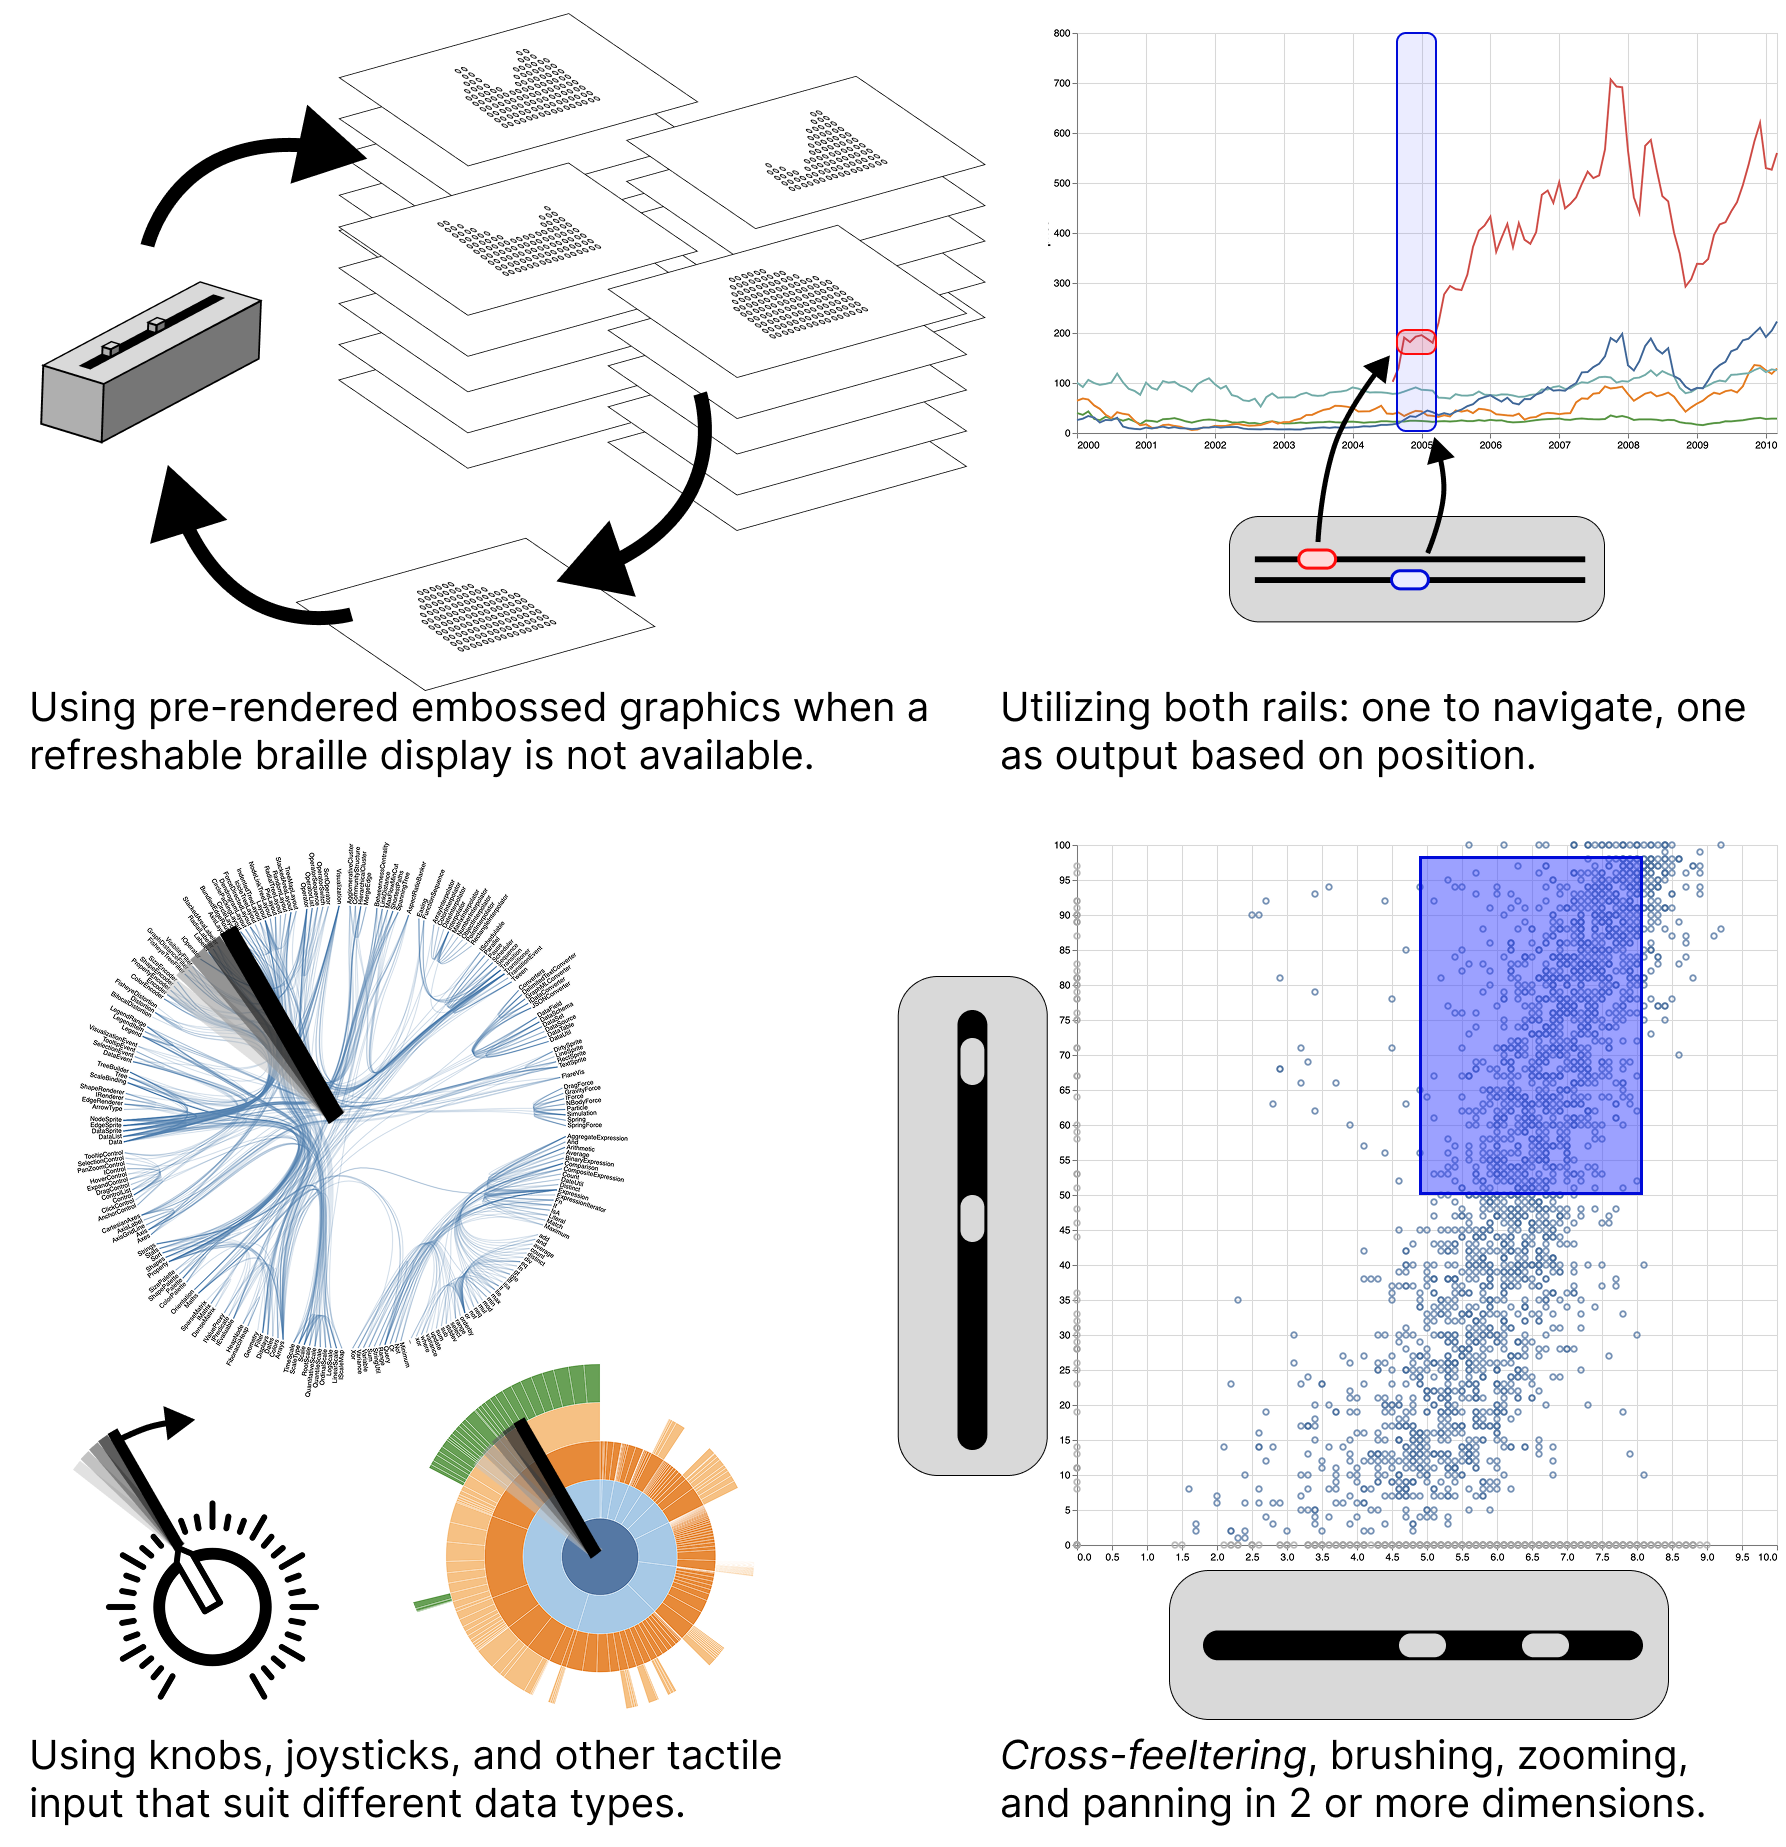
\includegraphics[width=0.65\columnwidth, alt={4 diagrams. 1. Using pre-rendered embossed graphics when a refreshable braille display is not available. A stack of embossed papers is being used with the feelter. 2. Utilizing both rails: one to navigate, one as output based on position. A line chart is shown with the 2-rail version of the feelter. 3. Using knobs, joysticks, and other tactile input that suit different data types. A knob is shown turning while a visual focus of the knob is shown over two complex circular visualizations. 4. Cross-feeltering, brushing, zooming, and panning in 2 or more dimensions. A scatterplot is shown being filtered with a square shape brush overlay. The overlay's 4 sides are controlled with 2 cross-feelters, one for each axis.}]{figures/future.png}
  \caption{%
  	Speculative future use cases for our \textit{cross-perception} approach, contributed by our participants.%
  }
  \label{fig:future}
\end{figure}

The following use cases were developed through the speculative futuring exercise~\cite{Dunne2013} conducted as part of our closing interview, with contributions from participants and the research team. We present them as design starting points grounded in the cross-perception framework, each addressing a limitation of the current prototype or extending the approach to new contexts. \Cref{fig:future} illustrates all four cases.

\subsection{Cross-Perception Without a Powered Display: The Pre-Rendered Interaction Cube} %

Refreshable braille displays remain expensive (\$8k--\$20k USD) and are not universally available. The current prototype depends on the Dot Pad to render cross-filter output in real time, which means the full cross-perception loop is unavailable to users without access to one.

One solution is to pre-render the interaction outputs for a given dataset before a session begins. The cross-feelter's filter operates over a bounded, discretizable range; it is feasible to pre-compute a set of interaction results at binned filter positions and emboss them onto paper as an ``interaction cube'' of tactile states, analogous to the data cube that Mosaic pre-computes for fast cross-filtering over large datasets~\cite{heer_mosaic_2023}. After each filter manipulation, the user turns to the corresponding page in a booklet of embossed tactile charts, reducing the interaction loop from 3--4 minutes (a full embosser render) to roughly 10 seconds. This approach trades the continuous, real-time update of the powered display for a discrete but physically permanent output, which has its own advantages for users who prefer to annotate or revisit prior states or even compare multiple outputs simultaneously, like in the dual-task comparison vignette in \Cref{sec:vignette}.

\subsection{Sequential Data Navigation with Continuous Positional Feedback: Feelter-Only Chart Interaction} %

Serial navigation of data arrays using a screen reader is slow because the user must step through observations one at a time without any persistent sense of their position within the full range~\cite{Elavsky2023}.

A single cross-feelter could replace this with continuous physical scrubbing. Most charts and datasets have finite, bounded observations in any given dimension; these bounds map naturally onto the full range of a fader rail. One rail would scrub through the ordered observations as the user moves the knob, with the screen reader announcing the current value. A second rail, motorized, would move its knob to a position encoding the corresponding value in a second data dimension, like a rising and falling bar in a bar chart.

More broadly, different input devices could be matched to different data topologies. A rotary dial would suit circular or periodic data (seasonal patterns, directional data); a joystick would suit data with an infinite or continuous range such as a parametric function or model output.

\subsection{Sonification Navigation via Physical Rail Position} %

Navigating within a sonification (seeking to a specific region, comparing two positions, returning to a reference point) is currently difficult even on touch-enabled devices, because scrubbing through audio provides no queryable positional state when the hand is not actively in contact with the surface~\cite{Chundury2022Towards, Chundury2024, Chundury2026}. This is the same object-permanence problem that motivated the cross-feelter's design for cross-filtering.

A cross-feelter rail could serve as the navigation input for a sonification: physical position on the rail maps to a position within the audio timeline or data domain, and the motorized mechanism maintains that position when the hand is lifted. The user can navigate to a region of interest, remove their hand, let the sonification play, return to the rail, and feel exactly where they left off.

\subsection{Multi-Dimensional Spatial Interaction: Rails as Input and Output} %

Two cross-feelter units, one arranged as an x-axis controller and one as a y-axis controller, could support spatial panning, zooming, and brushing over tactile maps or scatterplots, which are interactions that currently lack a satisfactory non-visual implementation because pinch-and-zoom gestures provide no queryable positional state for the zoom extent or pan position. Each feelter unit would maintain the current viewport bounds in its two rails, readable by touch at any time.

More substantially: the motorized rails could serve as \textit{system output} for spatial queries. When a user asks ``where is this object?'' of a map or image, the system could drive the rails to the corresponding x and y positions and bounds. This would let the user feel the location directly rather than receiving a verbal coordinate and build a spatial mental model of a spatial layout.

\section{Limitations}
\label{sec:limitations} 

Our study's controlled task design (three-minute timed tasks with multiple-choice answers) prioritized speed and query quantity, which are the right measures for a proof of concept but do not capture the full texture of blind data analysts' real exploratory workflows. Activities common in open-ended analysis, such as wrangling messy data, identifying outliers, and questioning assumptions, were not represented. An ethnographic or longitudinal study would be better suited to those questions, and we encourage that work. 

The Dot Pad's 500--1200ms render latency falls outside the max 500ms threshold at which Liu and Heer identify measurable degradation in exploratory analysis quality~\cite{Liu2014}. Our query count results are therefore a conservative lower bound on what cross-perception could support with faster display hardware. 

Novelty effects may have inflated subjective measures. The enjoyment and anxiety improvements may attenuate with extended exposure, though the effect may persist in contexts such as some classroom, work, or onboarding settings, where engagement is itself valuable. 

Finally, we compared against a screen reader baseline because screen readers are the dominant interaction tool for blind users working with data and all of our participants were proficient in screen reader use. More granular comparative work against other emerging tactile and voice-based input strategies would further characterize where cross-perception sits in the broader interaction space.

\section{Conclusion}
\label{sec:conclusion} 

We introduced cross-perception, a tactile interaction technique that adapts cross-filtering for blind data analysts by preserving the simultaneity of input and output perception that makes the technique analytically valuable. We formalized it through six design goals grounded in principles from visual analytics, spatial cognition, and blind information interaction; instantiated it in the \textit{cross-feelter}, a low-cost motorized fader device; and evaluated it against a screen reader baseline with 15 blind participants. 

In our study, Cross-perception substantially improves task completion speed, data query generation, and subjective experience, with particularly strong effects for participants without prior data expertise. The result that matters most is not the speed improvement but the query count: participants using the cross-feelter generated nearly three times as many analytical queries during open exploration, reflecting both a quantitative improvement and a qualitative shift away from navigating data toward interrogating it. 

We argue that analytical interaction accessibility---the capacity for blind users to filter, conjecture, and test hypotheses through direct manipulation---is an open research problem that deserves sustained attention as a primary site of inquiry, distinct from accessible rendering. The future use cases our participants proposed suggest that extending the design space to include hardware and physicalization opens directions that software-only approaches cannot reach.

\part{Personalization: System-building for User Agency}

\chapter{\textit{Softerware}: Enabling Personalization of Interactive Data Representations for Users with Disabilities}

\noindent\rule{16cm}{0.4pt}
\begin{quote}
This chapter was adapted from my published paper:
\begin{adjustwidth}{1cm}{}
% \-\hspace{2cm}
F. Elavsky, M. Vindedal, T. Gies, P. Carrington, D. Moritz, and Ø. Moseng, ‘Towards \textit{softer}ware: Enabling personalization of interactive data representations for users with disabilities’, \textit{Computer Graphics and Applications}, 2025 (to appear at \textit{IEEE VIS 2026}).
\end{adjustwidth}
\end{quote}
\noindent\rule{16cm}{0.4pt}

\begin{figure*}
\centerline{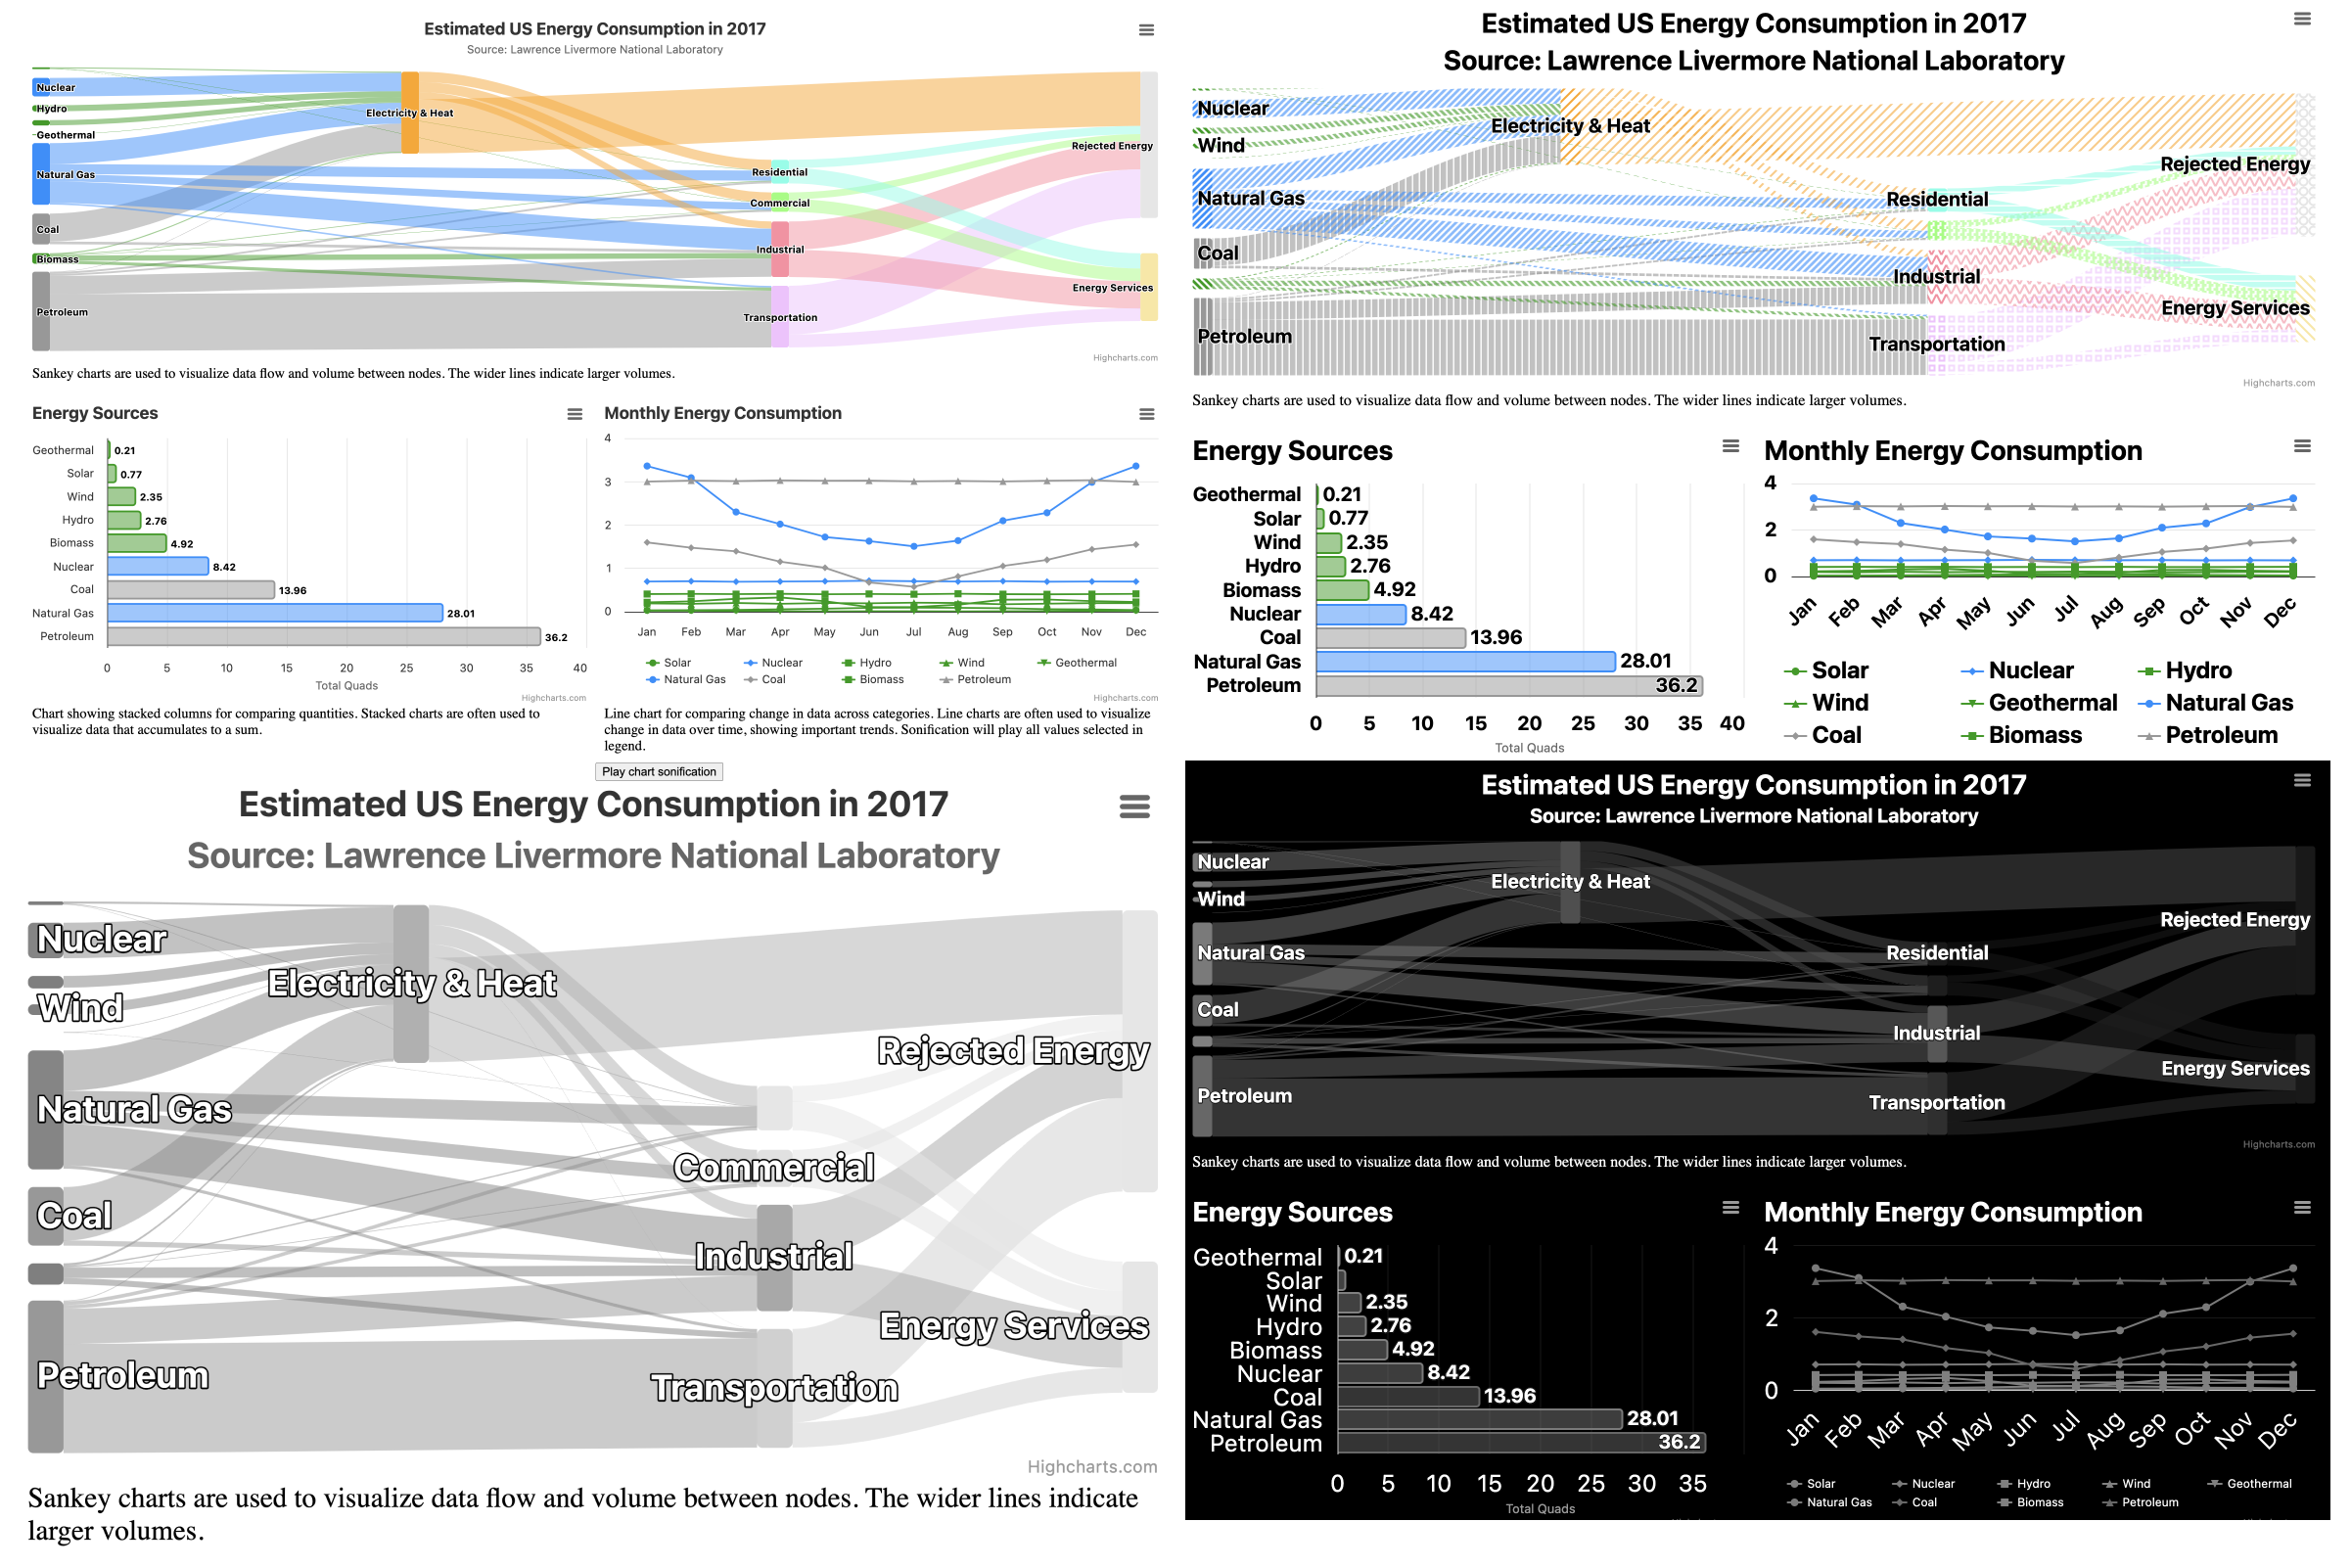
\includegraphics[width=0.8\linewidth]{options.png}}
\caption{Sometimes one design is not enough. Our design (upper left) and three different designs by low vision users. All low vision users chose larger text, but then diverged: redundant-encoding enabled (upper right), high zoom and greyscale on white (bottom left), and then dark mode (enabled externally) with greyscale (bottom right).}
\end{figure*}

\section{Abstract}
Accessible design for some may still produce barriers for others. This tension, called access friction, creates challenges for both designers and end-users with disabilities. To address this, we present the concept of softerware, a system design approach that provides end users with agency to meaningfully customize and adapt interfaces to their needs. To apply softerware to visualization, we assembled 195 data visualization customization options centered on the barriers we expect users with disabilities will experience. We built a prototype that applies a subset of these options and interviewed practitioners for feedback. Lastly, we conducted a design probe study with blind and low vision accessibility professionals to learn more about their challenges and visions for softerware. We observed access frictions between our participant's designs and they expressed that for softerware's success, current and future systems must be designed with accessible defaults, interoperability, persistence, and respect for a user's perceived effort-to-outcome ratio.

\section{Overview}
There is a significant and relatively unacknowledged problem in emerging work on accessible visualization: a single design cannot satisfy all users. People with disabilities, even those who share the same category of disability, often have different experiences, capabilities, and needs. As experienced practitioners and researchers who have been working to make data visualizations more accessible (some of us for more than a decade), we have each observed this persistent problem in our own practice.

Data visualizations that are produced by a designer for an audience tend to be designed in a way that is relatively \textit{unchangeable}. As a material, we use the metaphor that the creator of a visualization manipulated their design while it was in a \textit{softer} state, like clay. And eventually, the clay is \textit{hardened} into a state that is presented to the user. Often visualization design artifacts cannot easily be altered by an end-user after they are created. Pixels cannot be moved, graphics cannot be re-embedded. The clay has been fired and the visualization is now \textit{baked}. We intend to make visualizations easier to change and manipulate for end-users. We want a material that is softer than software. But we also don't want a fully malleable interface, like in end-user programming, either. We propose to call this space of design ``softerware.''

We wanted to explore material softness \textit{with constraints}. We conjecture that advancements in malleable interfaces and end-user programming are too system-centric and open-ended. End-user programming puts too much burden on end-users to know the language and symbols of interface-building in order to build their own interfaces. Instead, we chose to enable end-users to have agency over a data visualization interface by exposing a preferences-driven menu of options built from our existing knowledge of visualization and accessibility.

Exploring the \textit{softerware} gap in data visualization became our primary research focus, which led us to formulate the following qualitative exploratory research questions:
\begin{itemize}
\item \textbf{R1}: What constraints and capabilities should we provide end-users to give them meaningful agency over interactive data visualizations?
\item \textbf{R2}: What qualities, challenges, and design opportunities do designers and engineers envision for a data visualization \textit{softerware} system?
\item \textbf{R3}: What qualities, challenges, and design opportunities do blind and low vision users envision for a data visualization \textit{softerware} system?
\end{itemize}

We contribute our findings from this research to the larger accessibility and visualization communities in hopes that we can inform and inspire future work that investigates \textit{softerware} systems, end-user design, preferences-based user experiences, and fluid and malleable interfaces focused on end-users with disabilities. Our future work will focus on completing a finished version of our prototype and deploying it at scale within Highsoft's Highcharts ecosystem~\cite{Highsoft}.

\section{Related Work}
Our contribution is an attempt to bridge the gap between the knowledge we have on accessibility for visualization (as a complex space of design and engineering) with research and practice that centers on users with disabilities being able to adust, change, or control the interfaces they interact with. We intend to frame our work towards the benefit of data visualization designers, system engineers, and end-users of data visualizations. We believe that more flexible data visualization systems that enable user preferences will require a careful approach to architecture and thorough consideration for the burdens placed on end-users.

\subsection{Data Visualization and Accessibility}
Data visualization accessibility has come far in recent years. But little work has been done to explore what disability scholars call ``access friction'' - a tension that arises when access must be negotiated~\cite{Hsueh, Hamraie}. This friction is often a result of static barriers in shared spaces: one artifact or approach designed to include some people may end up excluding others.

In general, accessibility concerns itself with a broad spectrum of barriers that people with different disabilities face. And while most literature focuses on visual disabilities~\cite{Wimer, Marriott}, there are growing resources on areas such as cognitive/intellectual disabilities~\cite{Wu2021Understanding, Wood2024}, neurodivergence~\cite{Tran}, and both research and systems exploring epilepsy and vestibular/motion inaccessibility in visualization~\cite{South, Sivaraman}.

% access for assistive technologies that are used by people with dexterity and upper-body motor impairments~\cite{Elavsky2023}, 

Yet despite these resources, making data visualizations more accessible remains a difficult task for practitioners~\cite{Sharif2024Challenges, Joyner2022Wild}. Some accessibility guidelines even conflict, for example on the topic of patterns and textures used in charts. One side stresses that patterns are harmful to cognitive and visual accessibility~\cite{Schepers} while another stresses that redundant encoding strategies are necessary~\cite{Elavsky2022Chartability}. Understanding how to make the correct design decisions may sometimes be impossible. Either existing guidelines are incorrect or it is possible that access friction becomes inevitable the more we know what different barriers look like for different people with disabilities.

\subsection{Systems that Adapt}

One angle of exploration that has been engaging this issue already focuses on systems that can adapt. Work on adaptive systems for people with disabilities, such as in \textit{ability-based design}~\cite{Wobbrock2011}, stresses the importance of design alleviating burdens placed on users. Users who don't fit initial system designs are often expected to adapt to fit the system. This means that they may have to acquire an assistive technology, learn a peripheral skill, hack the system, or wait on a design fix. This places the burden on the user to fit the system. Ability-based design instead stresses that systems should be capable of automatically adapting, in order to reduce these burdens placed on the system's users. 

However, building data visualizations that automatically adapt to users via some form of data collection often do so through means such as monitoring live biometric data and input patterns, collecting a user's self-declared conditions and cognitive ability, parsing a user's history, and sensing a user's environmental or situational context~\cite{Yanez}. We argue that these methods for an adaptive system raise questions of end-user agency, trust, privacy, and awareness in regards to the system decision-making~\cite{Pallapa}. They may not be sufficient for addressing a user's needs while also preserving their privacy and agency.

\subsection{Personalization and Accessibility}
Lastly, we researched broader spaces where users have more design agency and explicit awareness of a system that is built to be adapted. We were interested in literature and projects that explore ways end-users can enact meaningful change on an interface, with special attention paid to accessibility and disability.

One specific project has emerged at the intersection of accessibility, visualization, and customization which focuses on screen reader users adjusting the content of textual tokens when navigating data visualizations~\cite{Jones2024}. While this is excellent work, we still have larger questions about when preferences, options, and customizations are appropriate and in what contexts as well as other ways of conceptualizing end-user agency over a system. It remains unclear when, why, and how customization and personalization can be used effectively when designing a system.

In the field of meta-design, meta-designers consider these end-user manipulations of a system to be one facet of ``end-user design'' and ``continuous co-design'' between a system and a user~\cite{Maceli2013}, which helps give us some meaningful language to refer to our system goals.

Recent work on the influential factors for personalization and adoption of accessibility settings~\cite{Wood2023} also informs our work in 2 key ways: conceptual mismatching between a system and user can contribute to a system's under-use while features that propose value, are time-saving, or reduce cognitive load for a user can contribute to positive perception and use of personalization of a system.

\section{Presenting: \textit{Softerware}}

\textit{Softerware} is a vision for software design that is not just based on giving a user the ability to set preferences or personalize. \textit{Softerware} is about the intentional design of a software system that enables people with disabilities to have meaningful, opinionated, and persistent agency over that system.

We contribute the concept of \textit{softerware} to the larger community of researchers and practitioners because we argue it is a useful construct that can help us categorize past work, improve existing projects, and inspire new directions. \textit{Softerware} systems have been part of existing work for decades, but we lack a cohesive way to refer to designing and engineering experiences that enable end-users to have agency over malleable interfaces without entering into the territory of end-user programming and end-user development.

\subsection{Defining \textit{Softerware}'s Principles}
Here we present the principles that define \textit{softerware} before demonstrating an example instantiation in the context of online, interactive data visualization.

\subsubsection{Principle: Has Reasoned, User-centered Constraints}
An important aspect of \textit{softerware} is that it is \textit{softer} than software (which is already-baked) but not quite as \textit{malleable}, free, and potentially low-level as systems that facilitate fully realized end-user programming and development~\cite{Ko, Cabitza}.

End-user programming is still a form of \textit{programming} in the end. It focuses on taking constructs, functionalities, and reasoning from software programming and development and presenting these elements to users in ways that may suit a user's natural language or mental models, such as through no-code, visual-only, or low-code approaches. We anticipate that many users, especially those experiencing accessibility barriers, will have difficulty interacting with software paradigms based on end-user programming and development.

Instead \textit{softerware} engages this limitation through reasoned constraints that leverage conceptualizations and language focused on overcoming anticipated user barriers. Providing constraints and then framing and presenting those constraints in ways that have vocabulary correspondence to user needs is what separates \textit{softerware} from existing work and literature on end-user programming and development.

To accomplish this, the \textit{softerware} system designer must work to anticipate not only what their system should do in a default or beginning state but also which ways that system will potentially fall short and require fitting by the end-user. The system designer should motivate all of the capabilities of a \textit{softerware} system based on what they anticipate users will want to change, how users can discover that change is possible, and then how best to enable users to enact that change easily.

\subsubsection{Principle: Facilitates End-user Agency}
\textit{Softerware} is ultimately about the process of architecting and implementing a system that enables an end-user to be able to easily express meaningful changes to that system's appearance and behavior.

Accessibility has been framed as a tension between fit and scale~\cite{Hickman}, where \textit{fit} refers to a system that is perfectly complimentary and synchronized to a user and \textit{scale} refers to a system that is capable of reproducing functionality for many different users. We believe that the tension between fit and scale, in addition to \textit{access friction}, can both be alleviated when a system is designed to facilitate end-user agency.

The cornerstone goal of a \textit{softerware} system is an attempt to facilitate \textit{self-fitting} at a minimum, and in ideal circumstances also facilitate social methods of sharing fitting (such as loading profiles or ingesting metadata from others).

\subsubsection{Principle: Demonstrates Value}
Existing literature makes one thing particularly clear when it comes to personalization and end-user design: it has to be worth it~\cite{Wood2023}. Users must be able to recognize barriers, issues, or shortcomings of a system and then discover and utilize capabilities provided to them to eliminate or alleviate those barriers.

This entire process must not be too burdensome and the payoff should establish an expectation that future use of the system will be improved. The time and effort it takes for a user to fix a problem should be less than the time and effort generated by that problem. This means that \textit{softerware} systems can likely be optimized and improved significantly over time, as better techniques are developed to perform tasks as quickly and easily as possible.

The user should also be able to validate the value of their interaction with a \textit{softerware} system through the continued use of that system. If something was a painful experience and they took action to alleviate that issue, they should be able to observe the effects easily.

\section{Prototype: Visualization \textit{Softerware}}
\begin{figure*}
\centerline{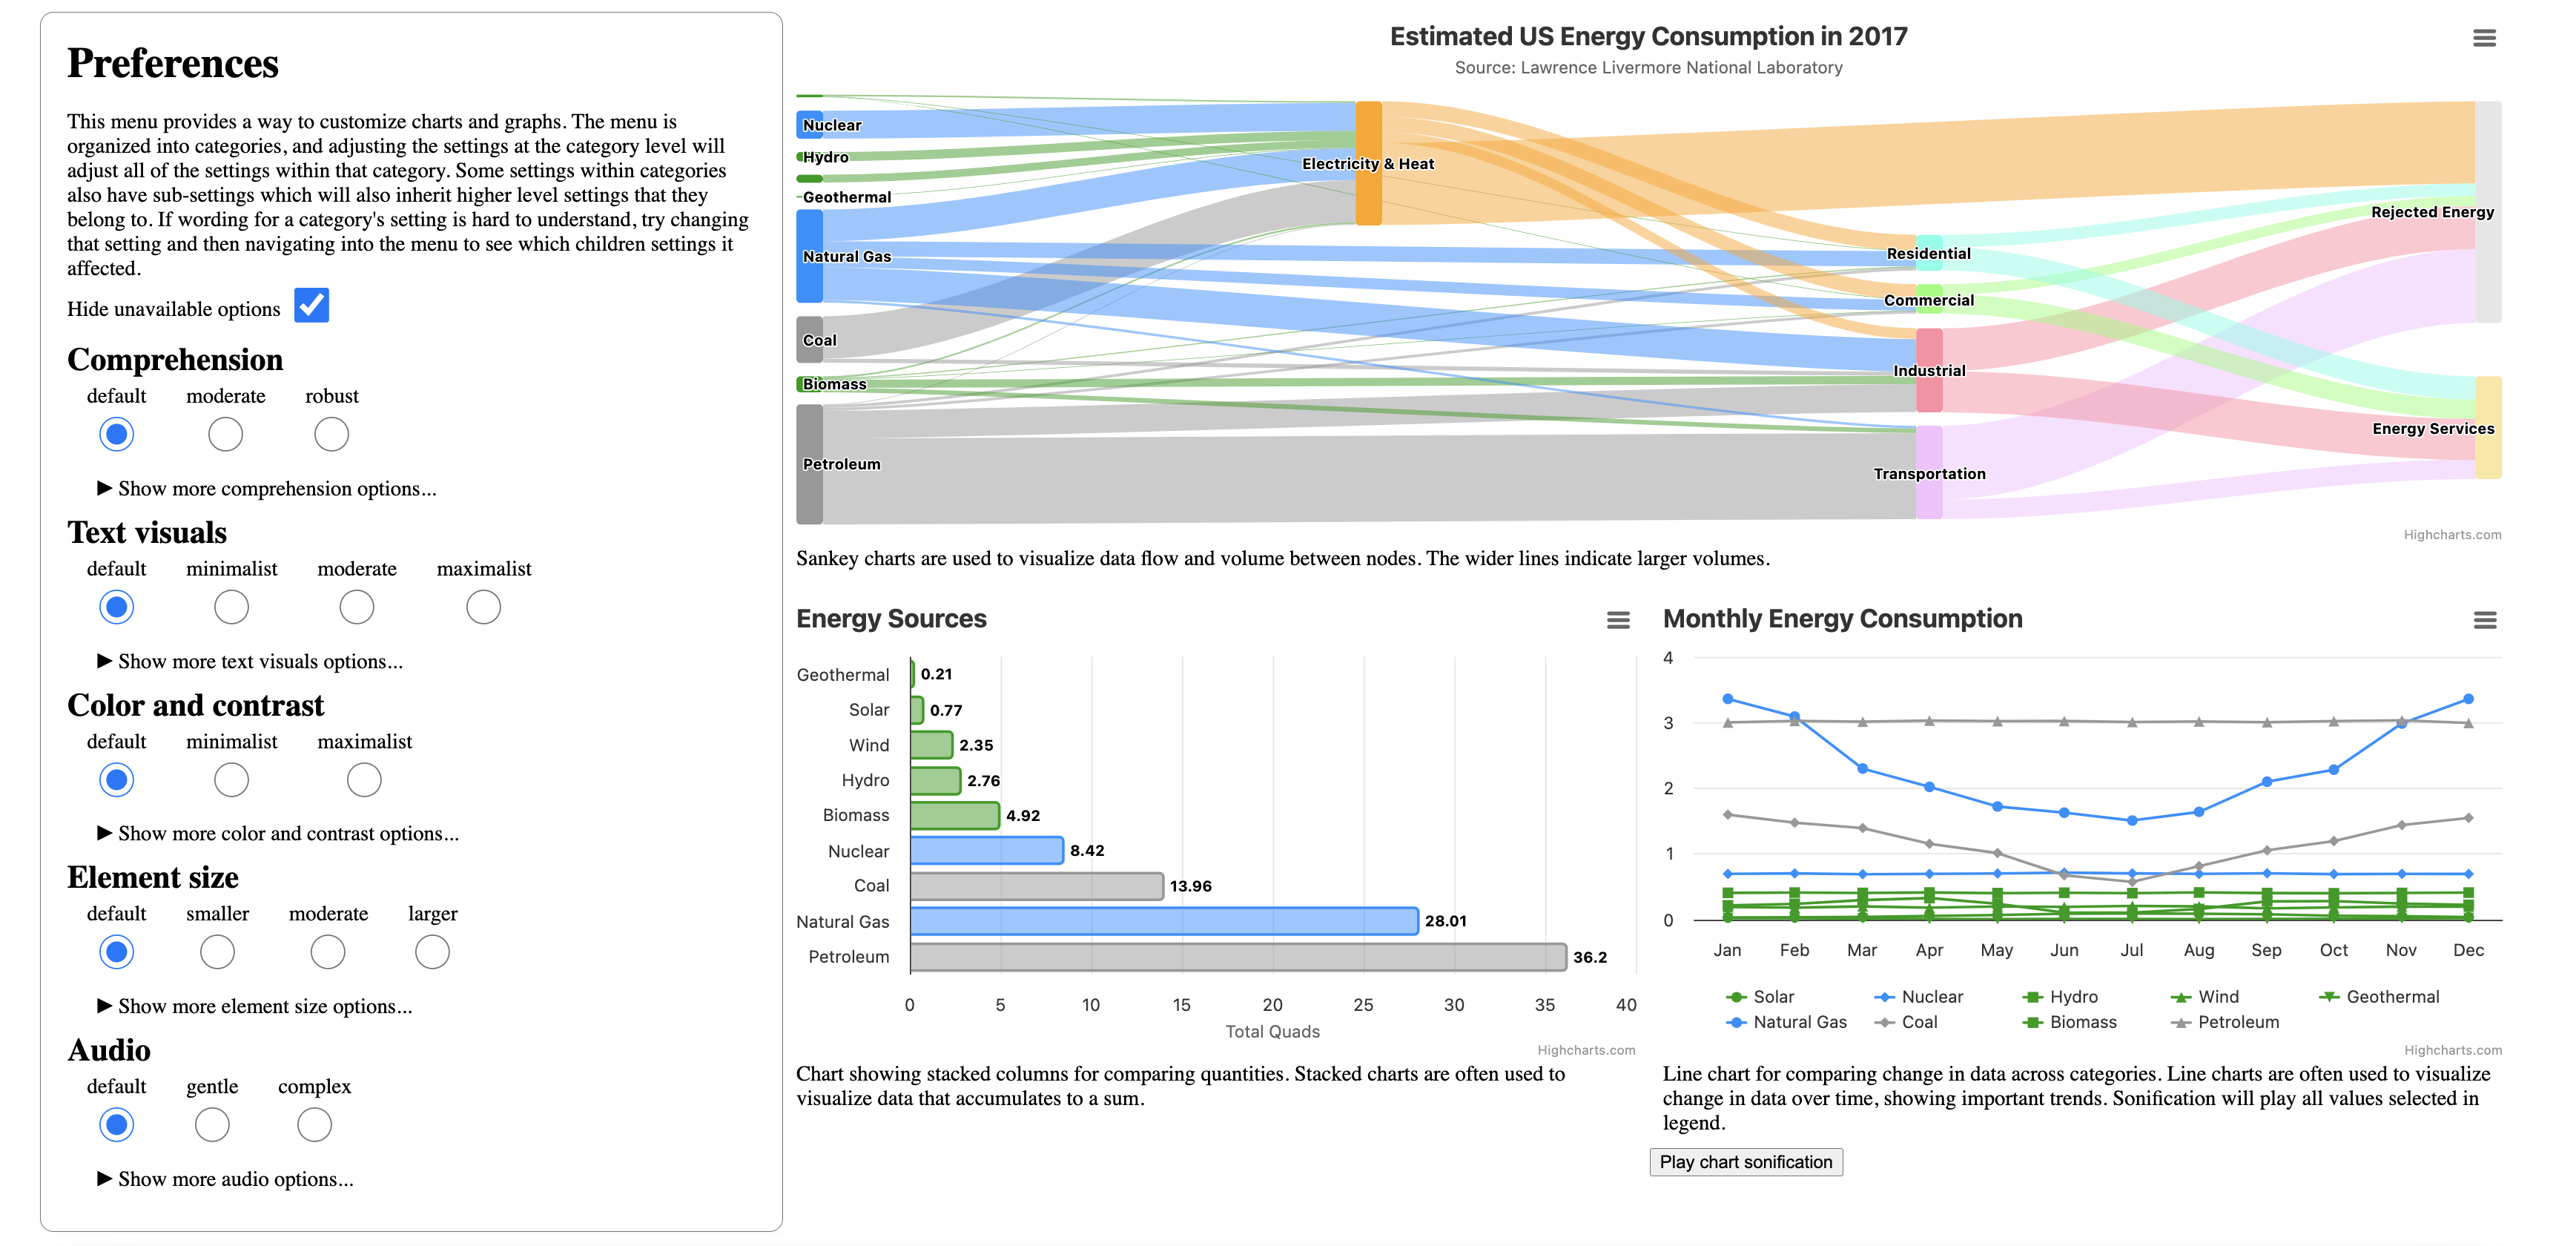
\includegraphics[width=38.5pc]{dashboard.png}}
\caption{Our dashboard design on US Energy Consumption in 2017 with a sankey, bar chart, line chart, and preferences menu on the left.}
\end{figure*}

We first built a data visualization dashboard (see {\bf Figure 2}) that would allow us to build a \textit{softerware} system prototype that we could demonstrate to designers, engineers, and evaluate with end-users with disabilities. You can view and interact with our prototype, including view our \href{https://github.com/highcharts/highcharts-a11y-prototyping}{open source code and dataset on user preference options, on github}.

We chose a relatively clean and standard dataset that would be relevant to our target end-users, who we would recruit from the United States, on 2017 US energy consumption. This dataset afforded us enough complexity to build multiple data visualizations in one dashboard (including an uncommon type like the sankey). This choice also allowed us to explore more ideas for user interventions and investigate broader questions in our eventual study. Our dashboard was built in JavaScript and laid out in a wide format for interacting with on a desktop machine.

We designed the dashboard to contain some interactivity, but nothing highly complex. Each chart has tooltips and visual filtering provided on hover/keyboard focus and the line chart has data filtering through the legend as well as sonification.

\subsection{\textit{Pretty Accessible} by Default}
In order to really test \textit{access frictions}, we wanted our dashboard to be considered accessible in its default state. We ran manual and automated tests according to accessibility standards as well as a 50-heuristic manual accessibility evaluation specific to interactive data visualizations~\cite{Elavsky2022Chartability, WCAG}. In addition, we chose to use Highcharts to create the visualizations in our dashboard because existing work has demonstrated the breadth of their accessibility capabilities~\cite{Kim2023Beyond}.

We ensured that text contrast was strong, text size was well above guidelines, interaction targets were of a minimum size, screen reader access was descriptive and interactive, our DOM was structured into a hierarchy, we provided semantic HTML data tables for each chart, and there were no \textit{critical} issues detected when running automated tests using \textit{axe DevTools} software. Many of the capabilities that made our dashboard accessible were provided out of the box by Highcharts.

\subsection{Reasoned Constraints: 195 Accessibility Options for Interactive Data Representations}

After building our initial dashboard (see Figure 2), our research team collaborated and discussed potential access frictions that might arise from the use of our dashboard. We used our existing experience from accessibility work, more than a decade in the case of the Highsoft and Elsevier co-authors, to assemble a list of concrete, expected user barriers that would be hard to resolve in a single design, and organized those barriers based on common themes.

We then used these themes to brainstorm how we anticipated end-users would identify barriers and then what language they might use to describe an identified barrier and overcome it. One example might be under the theme ``hard to see'': ``I can't read this text'' as a barrier with the final language for them overcoming that barrier as an expression similar to, ``I wish this text size was larger'' or ``make this text bigger.''

From these solutions, we re-framed the language into interactive option categories. All categories were given binned options and not more than 7 choices, to avoid overwhelming users. For example, ``text size'' was an option category and had 7 binned choices from ``small'' to ``large'' available. We then created a hierarchy of option categories underneath these higher-level categories which could allow for more element-level specificity within a data visualization. So ``text size'' as a higher level category with options also contained children that had more specificity, such as ``title text size,'' ``legend text size'' and so on. The final stage of our language and options design was in line with prevailing industry wisdom, which was to avoid organizing the language of our configurations based on categories of disability~\cite{Bailey} and instead focus on higher-level categories of identifiable elements of a user's experience, such as ``text visuals,'' ``audio,'' and ``color and contrast.''

At the end, we produced 195 option categories and 774 total option choices. Using the combinatorial rule of product, we calculated 6.83e114 possible unique end-user design configurations from these choices, which is more than the estimated number of atoms in the universe. 

However, to ensure the scope of our user study was feasible, we reduced our initial working option categories down to 33 with 137 total options (and 9.35e19 possible design combinations), all focused on options we believed would be most relevant for users who are blind or low vision. These options and our subset are viewable in \href{https://highcharts.github.io/highcharts-a11y-prototyping/early_explo/examples/menu/menu.html}{our live, interactive demo} online.

\subsection{Preferences Menu Design}
We then iterated on visual and functional designs to allow users to actually interact with and enact these design configurations. Our early ideas included a natural language interface (since we used a relatively ``natural language'' centered process to develop these categories), direct manipulation of the elements in a visualization (through focus, hover, click, or selection methods), and eventually settled on the user interface of a separate, visually nearby menu with nested options (see Figure 2). We designed our menu so that manipulating higher level options in the hierarchy would enact downstream options to follow suit, but any manipulation to downstream options would override higher controls, following common patterns used in systems that implement hierarchical specificity.

We justified our user interface as a menu for our final choice because it provides a place for metadata from the other design ideas (natural language and direct manipulation) to live, in case we develop those down the line as well. We anticipated that a menu not only provides a means of interaction but also storage of the state of a system. In addition, this type of user interface is common and relatively recognizable.

\section{Evaluation}
Our first research question for this project (``What constraints and capabilities should we provide end-users to give them meaningful agency over interactive data visualizations?'') focused on our thematic collation and compilation of anticipated access frictions, but our following two research questions would require outside evaluation: ``What qualities, challenges, and design opportunities do designers and engineers envision for a data visualization \textit{softerware} system?'' and ``What qualities, challenges, and design opportunities do blind and low vision users envision for a data visualization \textit{softerware} system?''

\subsection{Preliminary: Visualization Practitioners}
The preliminary step in our evaluation was to investigate what qualities, challenges, and design opportunities data visualization engineers and designers envision for a \textit{softerware} system.

\subsubsection{Recruitment}
We recruited 4 data visualization practitioners, each with roles as a current or former visualization software engineer (3) or designer (1). We recruited participants from our existing network of engineers and designers, requesting participation via email. Our practitioners were not compensated for their participation and we asked them up front if they would be willing to volunteer their time for us.

\subsubsection{Procedure}
We conducted 30-minute, semi-structured, qualitative interview sessions either over Zoom or in-person. The session consisted of a 5 minute explanation, 5 minute demo of our prototype's capabilities, and a series of open-ended, semi-structured questions for 20 minutes. Our questions started with getting their thoughts on the idea, what they anticipated other developers and designers would think, what aspects of a visualization they believe end-users will want control over, issues they believed end-users would face, and what new opportunities they envision our prototype and underlying design concept of \textit{softerware} enables.

\subsection{Study: Blind and Low Vision Users with Accessibility Expertise}

Our primary study was focused on our third research question on the qualities, challenges, and opportunities that users with disabilities, in this case users who are blind and low vision, envision for a \textit{softerware} experience of interactive data visualizations. To explore this, we used our prototype dashboard as a design probe to stimulate concrete feedback and ideation on both the details of our prototype as well as our larger design concept of \textit{softerware}, borrowing from Noor Hammad's method used when exploring accessibility preferences of users in novel streaming software~\cite{Hammad2024GameAware}.

Our study is intended to contribute qualitative knowledge, largely because we believe that statistical generalizations or controlled experiments about a particular group or subgroup of people with disabilities may actually produce knowledge that reinforces the existing problems we are trying to address. Instead, we are explicitly interested in knowledge and experiences that might exist on the margins, even knowledge as specific as a single individual's preferences. We want to explore ways that broader guidelines and design knowledge are capable of producing artifacts that still retain barriers for some individuals with disabilities. This larger challenge (of general guidelines that do not provide a meaningful fit for individuals living with disabilities) is not new to accessibility and assistive technology research~\cite{Power2012Guidelines}.

And to this end, we designed our study to maximize the production of knowledge that is considerate and careful of individual differences, challenges, preferences, and envisioned opportunities.

\subsubsection{Recruitment}
\begin{table}
\caption{Study Participants}
\label{tab:participants}
% \tablefont
\begin{tabular*}{18pc}{@{}llll@{}}
\toprule
PID & Age & Gender & Disability \\%                                   & Tech                \\
% \colrule
P1  & 39  & F      & Totally Blind \\%                                & NVDA, Windows       \\
P2  & 38  & F      & Totally Blind \\%, Left Arm Motor Impairment \\%     & JAWS, Windows       \\
P3  & 46  & M      & Legally Blind \\%Blind w/ Partial Light Perception \\%            & ORCA, Linux         \\
P4  & 28  & F      & Low Vision \\%, Light Sens., Nightblindness \\%      & Magnification, Mac  \\
P5  & 34  & M      & Legally Blind \\% & Various, Windows    \\
P6  & 52  & M      & Totally Blind \\%                                & JAWS, Windows       \\
P7  & 56  & F      & Low Vision \\%, Glaucoma (both) \\%                  & NVDA + Mag, Windows \\
P8  & 36  & M      & Low Vision \\%, Cataracts (both) \\%                 & Various, Windows   
P9  & 55  & M      & Totally Blind \\%, Cataracts (both) \\%                 & Various, Windows   
\end{tabular*}
\end{table}
Our study involved 9 total participants who are blind or low vision (see \textbf{Table 1}), all of whom are also professionals with accessibility expertise (either currently or formerly employed in an accessibility-specific role as subject matter experts). 5 of our participants self-identified as male, 4 as female. Average age of our participant group was 42.67 (SD = 9.99). We initially recruited 6 participants using an existing, compensated research relationship between Highsoft and an external consultancy. In addition, we recruited 3 more participants from our existing network of accessibility consultants, who were each compensated 100 USD for their time.

We anticipated that recruiting participants who not only have lived experience with a disability but also are subject matter experts in accessibility would contribute to the depth of our qualitative study as well as general breadth of considerations. We wanted to maximize the value of feedback on our work.

We reached out to all participants via email with a call for participation and participants were screened according to whether they are blind or low vision. Participants were notified in advance of compensation and that consent to participate is voluntary.

\subsection{Procedure}
Our qualitative study sessions were recorded and conducted over zoom in 3 primary phases (plus a break) during one 90 minute session. Our phases were: early interview, task-evaluation of our dashboard (menu hidden) with discussion, a break, and task-evaluation of our dashboard (menu shown) with final discussion.

\subsubsection{Introduction and Early Interview [20min]}
Our session opened with an introduction to the research team and gathering verbal consent from participants for participation. We gathered demographic information from participants and asked them about their current assistive technology use. We followed up with questions related to whether or not they customized their technology in any way, through adjusting settings, modifications, adding scripts, getting extensions, or equivalent. We then ended the opening session with ice-breaker questions about whether they can recall a chart or graph they have experienced in the past and what their favorite way to experience a chart is.

\subsubsection{No Menu Prototype, Tasks, Discussion [30-35min]}
The next phase of our session involved showing participants our demo environment (see Figure 2), except that our preferences menu was hidden. We explained what the dashboard was and entailed, including explaining each chart type shown (sankey, bar, and line) and how to read them. We gave users a short amount of time to explore the dashboard, and then notified them that in order to evaluate the effectiveness of our technology, we would be asking them to perform 2 data tasks, one elementary and one synoptic~\cite{Aigner}. Our intention for performing tasks was not to measure speed or accuracy of the participants, but simply as a probe for eliciting feedback on the usability and effectiveness of our prototype and design.

Our first question was to answer an elementary analytical task (direct or indirect lookup), ``Does petroleum or nuclear contribute the most to Electricity and Heat?'' (``nuclear'' was correct). Our second was a synoptic task (pattern identification or multi-value comparison), ``Which energy type has the highest use in Dec \textit{and} Jan?'' (``natural gas'' was correct). We gave participants a limited time (5mins total) to answer the questions and upon answering, we gave them the correct answer and asked them to explain their process of finding their answer, step-by-step.

Our final step in this process was to interview them about their perceived challenges and frustrations with the dashboard and whether anything could be changed or adjusted in order to help them complete their tasks. We followed this phase with a 10 minute break.

\subsubsection{Menu Prototype, Tasks, Discussion [30-35min]}
We opened the final phase of our study by sending our participants a new link to a version of our online dashboard that included our preferences menu. We explained the purpose of the menu and gave them 5 minutes to explore the available options.

After participants explored the menu and its effects, we repeated our tasks procedure. Participants were given 2 tasks to complete in five minutes. First, an elementary analytical task, ``Where does most coal go?'' (``electricity and heat'') and then a synoptic task ``In the summer, June through August, which energy type has the highest consumption rate?'' (``petroleum'').

Our final discussion focused on investigating our participant's thoughts on our prototype, the idea of preferences and customization, why they chose the customizations that they did, whether they had any new or additional ideas, considerations for other users with disabilities, and any other concerns, challenges, or feedback. We asked them specifically to consider both their personal, lived experience with their disability and assistive technology in addition to their professional expertise in accessibility.
% \begin{table}
% \caption{Technology Use}
% \label{tab:use}
% \tablefont
% \begin{tabular*}{18pc}{@{}lll@{}}
% \toprule
% PID & Technology & Custom? \\%                                   & Tech                \\
% \colrule
% P1 & NVDA, Windows & Yes      \\
% P2  & JAWS, Windows & Yes      \\
% P3  & ORCA, Linux  & Yes       \\
% P4  & Magnification, Mac & Yes \\
% P5  & Magn., Browser Ext., Windows & Yes   \\
% P6  & JAWS, Windows & Yes      \\
% P7  & NVDA, Magn., Windows & Yes \\
% P8  & Magn., Sys. Contrast, Windows & Yes  \\
% P9  & JAWS, Windows & No 
% \end{tabular*}
% \end{table}

\section{Results}

We performed two analyses from our studies, first analyzing our findings from our preliminary study from practitioners and then analyzing our results from our study with end-users. We collated our notes and transcript materials, coded them thematically, and then used affinity diagramming to group the themes that emerged from our data~\cite{Harboe}.

\subsection{Preliminary Findings}
To avoid repeating information between our preliminary study with visualization practitioners and final study with blind and low vision participants, any findings from our end-users that are echoed by our practitioners will be mentioned later. Only the findings unique to our preliminary study will be included here.

\subsubsection{Alleviating Situational Barriers}
3 of our 4 practitioners spoke about the potential benefits of end-user manipulation of a visualization for situational or contextual reasons. One participant gave the example that when giving a presentation using an existing dashboard, having the ability to manipulate features to suit layout, flow, and interactions on-demand would be valuable. Another example given was that at times a user's viewing device (such as a smartphone) can cause barriers, so softerware would be useful to have available.

% , mirroring sentiments from existing literature on the benefits of accessible technology for situational barriers faced by people who are not disabled~\cite{Wobbrock2019}

\subsubsection{Creating Potentially Harmful Visualizations}
The second theme from our practitioners (3) was the concern that end-users would be able to create a misleading or harmful data visualization. For example, we have studies on how encoding area size~\cite{Lo} and aspect ratios~\cite{Ceja} can be misleading or deceptive, yet being able to manipulate these for accessibility and contextual barriers (such as viewing a chart designed for desktop on a mobile phone) are important design considerations. Users may accidentally adjust features of a visualization while self-fitting that actually create problematic designs. Being able to design a system to avoid this would be important.

% Area size sometimes affects users with upper body physical or motor impairments (such as those with tremors) when a chart is interactive with a pointer, while aspect ratios are important for users with low vision being able to adequately find and compare visualizations and see visualizations when using high levels of zoom.

\subsubsection{Designing via \textit{Softerware}-first}
The final theme from our practitioners was around authoring and design-tuning via \textit{softerware}, where 3 participants discussed using a direct-manipulation or LLM-based \textit{softerware} interface to author data visualizations and 1 of the 3 also mentioned that large-scale, privacy-preserving data collection from users could be used to create smarter design defaults in the future. We believe that both suggestions mirror existing work that speaks of the benefits of ``design-through-use'' and ``continuous-co-design''~\cite{Maceli2013}.

\subsection{Prototype-level Feedback}
The advantage of a study with participants who had accessibility expertise in addition to their lived experience as people who are blind or low vision is that we were able to get feedback on our existing prototype as well as on our larger idea space for \textit{softerware}.

\subsubsection{Navigation Structure Options}
While not a theme across participants, P2 mentioned that they would like to be able to navigate a data visualization using headings with their screen reader, rather than via regions. (``Regions'' are a type of semantic markup used to create programmatically recognizable organization for screen readers.) This was a suggestion that immediately led to our team iterating in parallel on ideas the next day. More than 71\% of screen reader users navigate information via headings when first encountering a new web page~\cite{WebAIM}. This suggestion made sense to explore as a sensible default.

\subsubsection{Previewing Change}
Our low vision users (P4, P7, P8) requested a feature that we had originally designed but not implemented, which was to directly show what different options would look like in the preferences menu itself. For example, the ``text size'' options would either have a preview of the text size shown for each option in the menu (like showing ``Large'' in the actual resulting large text size) or with a nearby preview window that would show the result of a selection as it is being selected. Low vision users in particular often use high levels of magnification and zoom, so the live results shown in the visualization space required users to go back and forth between the menu once an option was chosen and into the chart space to find what had been affected.

\subsubsection{Language Re-consideration}
Some of our participants (P1, P2, P4, P6, P7, P8) noted ambiguity or lack of clarity in the wording we used for our menu's higher level options, such as ``Audio'' having options for ``default,'' ``gentle,'' and ``complex'' while lower level options that inherited these were hard to connect to. For example, ``Sonification order'' under ``Audio'' had the options ``default,'' ``sequential,'' or ``simultaneous.'' ``Gentle'' in ``Audio'' would set the child setting for sonification order to ``sequential,'' but this was unclear initially.

Other participants (P1, P2, P3, P6) noted that while the menu's focus on functional categories was helpful, it might be nice to also have a way to customize the menu itself or view it from a ``disability'' perspective, so they could get all the screen reader options in a single place. Users were interested in looking at all options relevant to ``screen readers'' or ``low vision'' together.

\subsection{System-class Accessibility Findings}
The next set of themes that emerged were considerations that both our end-users and our visualization practitioners shared, which we are calling \textit{system-class} considerations, using the phrase from Chris Fleizach and Jeffrey Bigham~\cite{Fleizach}. In order for \textit{softerware} to function at scale, certain technical and infrastructure considerations would have to be prioritized to make things possible. This theme emerged thanks to the accessibility knowledge and expertise of our end-users and engineering concerns of our practitioners.

\subsubsection{Persistence}
Every participant (P1, P2, P3, P4, P5, P6, P7, P8, P9) as well as all of our practitioners noted that the ability to create some sort of ``profile'' or persistent state of their customizations would be one of the most important features that would make \textit{softerware} actually useful.

\begin{quote}
``What if I come back to this? Will I lose this? Do I need to do it again?''---P6
\end{quote}

We followed up by asking whether certain contexts would make persistence more or less important. We asked users whether a random website or news article with a chart in it would be worth their time, to which most users replied, ``no.'' However, P5 noted that ``This is so fun that if it was there I still might play around with it and use it, especially if I had the time.'' P4 related this issue to an existing frustration with video games, noting that having to set up repeated options for every game was time consuming. It would be nice if they could ``do this once and forget it.''

\subsubsection{Profile Sharing}
Following this theme of establishing a profile, most of the participants (P1, P3, P4, P5, P6, P8) and 2 of our practitioners also expressed interest in being able to share their own profiles or ingest settings from others, in order to save others or themselves time. In phase 1 of our procedure, we asked users about their existing levels of modification, customization, and preferences setting in their existing use of technology. While all of our participants (except for P9) customize, personalize, or modify their technology to some degree, those who were most interested in customization or spoke the most about it (P3, P4, P5, P8) were also the most passionate about being able to save \textit{other} people time and not just themselves.

\begin{quote}
``I customize my tech a lot. If I use something for the first time and it feels off, I find a way to fix it. But most people aren't like that; it takes too long. So I love when I can share [my modifications and customizations] with others.''---P3
\end{quote}

\subsubsection{Cross-system Interoperability}
Closely related to \textit{persistence} and \textit{profile-sharing} was an idea expressed by several participants (P3, P4, P5, P7, P8) that they wanted to be able to use these settings outside of Highcharts and even outside of the web. ``Will this work in Microsoft Excel?'' and ``I use salesforce for analytics a lot and would love this there,'' remarked P4. However, cross-system interoperability would require multiple charting libraries being intelligent enough to ingest user settings, when most are currently incapable of even recognizing a system's ``high contrast'' settings being active. In addition, all 4 of our practitioners suggested that there would need to be a system in place, either at the operating system level or as some kind of service hosted by a platform, where these settings could be recognized and ingested. For cross-system interoperability to be made possible, it would require establishing standards for customization, standards for preserving user privacy, and coordination with the larger community of visualization practitioners and software providers.

\subsection{User-Centered Findings}
The last major set of themes is related to the considerations of end user experience of a \textit{softerware} system applied in practice, including our observations about the differences between users and their choices when personalizing a data visualization interface.

\subsubsection{Frictions in User Differences}
Our first major user-centered finding was that no participant chose the same set of preferences as another. Every user discussed different reasons for justifying their choice of options. Users even chose options that others specifically emphasized were inaccessible to them. An example of this was a tension in preference for and against use of ``dark mode'' designs.

\begin{quote}
    ``If anything has dark mode? That's great. I wish everything used dark mode.''---P4
\end{quote}

P4 mentioned that they had ``night blindness'' (\textit{nyctalopia}), which is why dark mode designs are helpful for them. However, P7 also mentioned that they had progressive nyctalopia, but dark mode makes an interface ``virtually impossible'' to them.

\begin{quote}
    ``Oh, I can't use dark mode at all. I hate when websites have [dark mode] because it can be virtually impossible to use.''---P7
\end{quote}

Any one of the designs chosen by a low vision participant would have been insufficient for providing access for any of our other low vision participants (see Figure 1).

Our blind participants also had different justifications and preferences for their text and audio customizations. Some justified their differing preferences with similar justifications, such as cognitive accessibility and text description length. For example, P9 stressed that ``I prefer to keep things simple'' to ``avoid overwhelm'' while P2 said, ``more information is better than less, when it comes to data.'' Both P9 and P2 preferred ``accessible defaults,'' but disagreed on what length of textual descriptions should be default.

\subsubsection{Accessible Defaults are a Necessary Prerequisite}
Several participants were concerned that this approach would allow designers and developers to continue to make inaccessible charts (P2, P6, P7) if users have the ability to \textit{self-fit}. Participants emphasized how important it is to have strong accessibility \textit{before} customization is introduced (P2, P4, P6, P7, P9). Even 3 of our 4 of our practitioners expressed worry that \textit{softerware} could put a design burden on users.

P9, our only participant who almost exclusively uses default settings (and avoids mods and extensions) with their current assistive tech, stressed the importance of well-thought out defaults. It is clear that for users like P9 in particular, strong defaults are much more important than customization. Although less common, some assistive technology users are not interested in the work involved in personalization and would prefer technology to suit their needs out of the box.

This leads us to argue that there is a line between ethical use of \textit{softerware}, which is built on top of already-accessible material, and \textit{softerware} that is filling gaps in poor design. Designs that are lacking access that wouldn't cause any friction for someone else if they were present, such as simply having alt text, aren't in need of \textit{softerware}, they're just in need of accessibility.

\subsubsection{Effort-to-Outcome Ratio}
As a playful rephrasing of the visually-centric (and controversial) \textit{data-to-ink} ratio~\cite{akbaba}, we observed an \textit{effort-to-outcome} ratio among our participants, in line with previous results from existing work~\cite{Wood2023}. Nearly all participants (P1, P2, P3, P4, P6, P7, P8, P9) noted that the work required to interact with this menu wouldn't be worth the effort if they had to do it every time they interacted with a data visualization.

Most of our participants who used screen readers (P1, P2, P3, P6, P9) also mentioned that the menu itself was too cumbersome for navigating within and back and forth with the dashboard. Setting options was quite slow, and observing the output of a given option change, such as text verbosity or sonification type, was hard to do with accuracy. Keeping what a previous state was like in memory was hard.

One participant was interested in different ways that this process could become easier, suggesting

\begin{quote}
    ``What if I could just tell it what to change while I'm listening? Like right here [navigating a chart element] what if I could just say ``keep it short'' or maybe ``wait, tell me more.''---P6
\end{quote}

This suggests that there may be a space to explore non-visual direct manipulation \textit{softerware} strategies.

\section{Conclusion}
In an idealized world, designers do their best to produce useful and accessible interfaces. They're concerned with making software as accessible as possible by default. But no single design is capable of perfection. \textit{Access frictions} between accessible defaults and the needs of real individuals might always be present in software interfaces. To that aim, we hope to contribute knowledge that can inform future designers and developers to not only build accessible artifacts, but build \textit{systems} that enable end users with disabilities to have interactive agency over their software experiences.

Our vision of data visualization \textit{softerware} demands more involvement from research and industry. In order to offer as much value as possible to end-users, we need standards set for accessibility profiles and we need data visualization software, libraries, and applications to respect and be able to contribute to those profiles. We want to encourage researchers to investigate further the needs of people with disabilities, designers to imagine new interfaces and interaction paradigms for end users, and engineers to build robust systems that are capable of not only respecting a user's preferences and customizations, but providing persistence, interoperability, and system-class infrastructure.

\part{Conclusion}

\chapter{Discussion \& Future Work}

\section{What is a ``tool?'' A reflection on the social and material identity of tools}
In the introduction of this dissertation, I use the example of a hammer: a hammer can destroy and it can construct. So is the \textit{use} of a technology what constitutes it? Do we understand the hammer as the \textit{thing we swing, to destroy and to build}? Should we?

This thesis engages domains of tools and tool-making for accessibility: evaluation, navigation, interaction, and personalization. But these categories for work do not fully characterize the upstream conditions that our software systems and data interfaces inherit.

In my work specifically on accessibility, a larger social reality becomes apparent that shapes the question, ``what is a tool?'' far more than how an individual might use one, or the domains of work that our tool-making inhabits. My research journey has navigated multiple social and political thresholds, from changes to law in the European Union, to the enactment of Title II as part of the update to the Americans with Disabilities Act. These laws have motivated a significant interest in accessibility research, solutions, guidelines, and technologies. In the midst of this, we have seen the rise of overlays and generative AI solutionism~\cite{Hartman2025} and subsequent lawsuits and grass-roots resistance.

For my work, this is mostly good news. Legal change produces motivation, and even with predatory technology attempting to address real problems, pushback is widespread and active. But this paints a picture of the reality that my work inherits: many tools cannot even be used, or cease to be used, if there is not a social, political, and material set of conditions in place motivating those tools, providing resources for their construction, regulating their use, and examining the outcomes of what they accomplish. Tools and technologies are often a response to social, cultural, political, and legal realities that we first negotiate.

I recently spoke on this at a keynote in Australia, on how a hammer isn't \textit{just} a tool and that the idea that ``the only thing that matters is how a tool is used'' limits how we really understand tools. Instead, I spoke about how a standard, household hammer requires iron and wood. That alone leads to a whole universe of different questions. Western Australia's conservation efforts were disrupted when a significant amount of natural iron was discovered in a wildlife preserve. So laws were passed and now iron is mined there. That iron is largely exported. And Australia then, whether with Australian iron or not, mostly imports their small tools. Iron is sent out, and through a complex network of trade (likely indirectly related to the iron), hammers are brought in. A ``hammer,'' to even exist at all, relies on multiple levels of human governance, international relations, and complex infrastructures of trade.

And while my metaphor is largely motivated to encourage younger practitioners to consider the ``iron mines'' in the technologies they use, such as modern generative AI, it is also an area that is not adequately explored and addressed in terms of accessibility research.

Research on accessibility is dependent on funding, which is often dependent on political priorities and action. Depending on the current social and political state of the world at large, accessibility research itself may never gain the opportunities required in order to innovate and produce new tools at all. And as the US's 2025 federal cuts to research demonstrated, millions of dollars devoted to accessibility research can be lost to political agendas. It is for this reason that engagement with policy recommendation and guidance is essential. Personal political activity and involvement is also essential. Researchers who genuinely believe in accessibility as a human right or as a dignity that all people deserve should work with policymakers to ensure that there are material and structural resources in place for this work to continue. We cannot naively believe that technology, divorced from the realm of social and political forces, is capable of solving accessibility barriers~\cite{Spiel2020}. Without enforcement and threat of litigation, very little accessibility work has been accomplished in the past by technology companies alone.

Not featured in these chapters (as they were merely stapled in research papers from previous publications) is the policy and outreach work involved in seeing that work like \textit{Chartability} and \textit{Data Navigator} are used in real contexts, including by organizations that govern and influence the lives of many people. Immediate incentives to produce novelty may not be enough to sustain the larger socio-cultural and political ecosystems that our work participates in and is downstream from. We must also get involved.

\section{``Applied'' accessibility work and \textit{low research}}
I came into an academic research environment already as an engineer. I had questions to big problems, especially about how tools might shape human behavior and how we can use that towards ethically good outcomes. But \textit{Chartability} was a project I made first for myself, to engage the problems I, personally, was facing.

And \textit{Data Navigator} was motivated by my existing experience making visualizations navigable. I knew we had to build better tools, because continually trying to make a hierarchical substrate like HTML work for complex, non-hierarchical relationships simply limited what was possible and easy to do.

These two projects then led to many opportunities to test them in applied contexts. Our CZI grant was motivated towards the application of both, Adobe was interested in \textit{Data Navigator}, and the University of Wisconsin's GIS folks wanted to figure out how to make a complex map navigable, \textit{Data Navigator} or not. Yet, as a researcher I wasn't incentivized to pursue these projects. In fact, they all proved to have no immediately apparent novelty. It was a risk to spend my time in these spaces.

Applied work is structurally and socially devalued in academic research environments, seen often as a lower form of research and design compared to more ``pure'' forms of knowledge production. (I conjecture that in part this is due to the scope of knowledge that practitioners produce: they work to take broad knowledge and apply it to specific, small problem spaces. Foundational research tends to assume that broad knowledge does not then bubble up from this work, that it is a one-way flow.)

In my first year as a PhD student I was given the advice by a senior researcher not to hold my experience as a practitioner too highly because, ``practitioners often don't know what they are doing.'' But I did, of course, to some degree. Yet, this attitude is pervasive in some spaces and is a problem because it limits what kinds of knowledge we care to attend to.

Initially, I felt that with \textit{Chartability} I had lucked out. But after 4 more collaborations which resulted in funding and 2 research publications, I can now argue that this method has been reliable. In \textit{Softerware} and \textit{Skeleton}, pursing practical problems in applied environments \textit{did} serve as a fruitful source of generalizable knowledge and advancements in the state of the art. But these projects, in addition to \textit{Chartability}, were all motivated by immediate, non-novel problems: people knew their charts were inaccessible and wanted some design guidance or engineering solutions.

So perhaps ``low research'' works.

Yet some research communities, especially \textit{ASSETS}, have yet to reckon with ``applied'' work like this. If you trace the lineage of \textit{action research} from Hayes~\cite{Hayes2011ActionResearch} (which is how we frame our applied work in \textit{Skeleton}), it leads into fantastic areas of participatory and community-based work, often with or by marginalized people and people with disabilities~\cite{Spiel2020,Sum2024,Sum2022,To2023,Bennett2018Interdependence,Williams2023,Hsueh,Lundgard2019Sociotechnical,Mankoff2010Disability}. I would even argue that this lineage of work, which prioritizes and centers the lived experience of a person, is also why we have seen so many successful auto-biographical and auto-innovation styles of research as well recently~\cite{Seo2024,Biggs2022Audiom,Glazko2023,Williams2019,Williams2021,Gardner2023,Hofmann2020}.

And yet, action research largely does not touch on how practitioners (particularly those without disabilities) do applied work in accessibility~\cite{Joyner2022Wild,Sharif2024Challenges}. I believe that significant gaps exist in the space between traditional ``high'' knowledge production and applied, ``lowly'' spaces. Researchers tend to pursue novelty and the lifecycle of research production is highly risk adverse. And yet, relatively little work has been done within the accessibility research community to intellectually address the actual social and cultural risks involved producing decades of useless, lost, and forgotten prototypes and design guidelines~\cite{Hurst2013Making,Jackson2022}. I would conjecture that research-producing academics are overly concerned with academic readership relative to the myriad of ways that their knowledge production actually is used by the rest of the world~\cite{Mohammadi2015}. I would challenge \textit{ASSETS} and the AT/accessibility communities of \textit{CHI} in particular to take seriously the lack of applied (industry, government, and non-academic) work it produces as a community.

\section{Who is responsible for repair?}
Lastly, I want to revisit one of my opening points, where I argue that the \textit{tool-makers} are first responsible for repair. This is true. However, the most pressing issue I have faced in recent years is mostly unmentioned across these research projects: tool-makers might be responsible, but this is because they are the only ones who have the \textit{power} to make things accessible. Does this always need to be the case? Can we imagine an artifact's authority over the user's ability to access being designed towards self-subversion~\cite{Graeber2006} or de-centralized agency~\cite{Keyes2019,Mohan2000,Casey2018}, instead? What might that look like, concretely?

In \textit{Softerware}, we begin to engage this larger problem in terms of an idealized state where a user can repair or re-design their own experiences. But to me, this self-repair is like laying down train tracks for yourself as you move a locomotive, but then lifting up your own tracks behind you as you go. You're the only one helping yourself. This is not ideal, for you or others.

What we need are broad, lasting, infrastructural changes. On the web, this problem becomes quite difficult to solve. A personal computer or device? Again, someone can auto-design their interfaces into a better state. But back when I started \textit{Chartability}, the WebAim Million's report showed more than 95\% of the top one million website home pages contain at least one critical accessibility error. And now, more than 6 years later, that proportion is unchanged~\cite{WebAIMWebAIM}.

Some had imagined that generative AI would solve the massive infrastructural repair problems we face. But unfortunately, the latest WebAim Million report shows that since 2020, ARIA usage has increased and correlates to more errors, while use of tabindex on a page has increased nearly 300\% and also correlates to more errors on a page. If anything, during the age of generative AI, we have seen existing bad patterns worsen in prevalence and complexity.

I firmly believe that a tools-based approach is not enough on its own. Tool-making cannot be the \textit{only} intervention on inaccessibility. Tools and tool-making, as our thesis argues, have a powerful role to play. But we simply can't tool our way out of failed infrastructure and inadequate policy when someone else \textit{owns} the tools and tool-making. Visiting a website is like going into someone else's home: arranged according to their effort, tastes, and so on. If you can't access their home, you essentially need to request that they let you in personally. Website repair always falls to the owner and maintainer of a website, and they largely don't take any meaningful action.

Sidewalks outside of homes are a good parallel to this problem. Sidewalk accessibility is a massive infrastructural problem~\cite{Saha2019}, and yet localities treat sidewalk maintenance in different ways: some, like where I presently live in the south hills of Pittsburgh, put the onus on the homeowner whose house and property the sidewalk touches. In other places, sidewalks are considered a public path, similar to a roadway, and are maintained through public tax and resource management. To no surprise, privately-maintained, public-access sidewalks are worse for people in pretty much every way than publicly-maintained ones~\cite{Woldeamanuel2016}. This is because private homeowners don't care about sidewalk maintenance unless the city manages to fine them or they get sued.

And the web is a collection of private spaces that you visit privately. There is no truly shared, universally democratic, public space on the web. Centralization is partly to blame: sharing space while scaling leads to consolidation.

So my future work will continue to wrestle with the same tensions of scale, repair, and anti-consolidation of power, motivated by the same WebAim Million report. But now I look to questions of \textit{democratic} and \textit{radical} access to accessibility repair. The barriers I hope to tackle in the future are political and infrastructural. Perhaps tool-making will participate in this work, but it seems clear now from my work that the upstream technical problems and socio-political conditions that tools inherit, will likely not be addressed by tools alone.

What does ``democratic'' and ``radical'' infrastructure work look like? It will probably be an extension of \textit{Softerware}, to some degree. I imagine future research that explores public-first spaces, ones where access is socially negotiated and repair belongs to all of us. Is this an autonomous space, like an autonomous zone~\cite{Bey2003} separate from the web? Above it, looking down into it, like shared annotation tools but capable of sharing the manipulation of websites~\cite{RulandStaines2018}? A space with ambient co-repair, modeled after projects that bring people together~\cite{Shakeri2024} or that allow community ``fixing'' of misinformation~\cite{Jahanbakhsh2022}? Perhaps feminist thought on the ethics of care can help us~\cite{Henriques2025,Maeckelberghe2004}? Or maybe it will be something else entirely; I'm not yet sure. But what made the web fantastic years ago is long gone; most of it has been hedged into corporate spaces that are controlled, maintained, and repaired by corporate power. And these entities are notoriously bad at repair. What I imagine in the future involves reclaiming a sense that the web is \textit{ours}, belongs to \textit{us}, and that ultimately \textit{we} are responsible for making it accessible.

\chapter{Biographical Sketch}

Frank Elavsky was born in Seattle, Washington and grew up in Anacortes, to the north on Fidalgo Island. He was raised in poverty by a single mother on SSDI who lives with multiple disabilities; his father is multiply disabled and homeless. Frank himself has chronic pain and disability, as well as living with diagnosed and self-diagnosed neurodivergence. In his early years in school, he had alternative classes and behavioral interventions. In middle school, he began working on a fantasy world and tabletop game called \textit{Braven}. He was not a notable student in high school and did not receive honors. He was in and out of surgeries and the emergency room, missing over 180 days of school combined across his junior and senior years. At the time, he loved traditional art and was accepted into Cornish School of the Arts in Seattle. He could not afford to attend.

Upon turning 18 but before graduating high school, he was kicked out of his house by his mother, who had just sold his car for opiates. After several surgeries by his 19th birthday, his health significantly improved. He then worked several odd jobs (furniture mover, barista, carpenter, painter) until getting fired from a pizza shop at age 21. He crashed out and applied to a nearby liberal arts college, Trinity Lutheran, in Everett, WA. He was awarded a substantial scholarship. 5 years later he graduated Magna Cum Laude with two degrees, a B.S. in Computer Information Systems, and a B.A. in Theology and Philosophy.

While attending, he was committed to serving his peers as Student Body President and also did substantial work in his spare time as a community organizer, fighting for student, housing, and carceral justice at Trinity and in the Everett area. He married Shelby while attending Trinity, who was a close friend from home in Anacortes. Trinity closed as a college and became a foundation the year he graduated (2016), because students, staff, and faculty organized against corruption. (On rare occasions, Frank has been known to spill his insider-exclusive tea on all of this over drinks, with close friends.)

He then worked in industry, specifically in data visualization. His visualization work won several awards, even appearing (uncredited) in the 2017 Nobel Lecture on Physics by Barry Barish (see Fig 9 in~\cite{Barish2018}). Despite this, he was always terrified with impostor syndrome.

At 31, he left a well-paying, comfortable career with excellent health insurance and started his PhD at Carnegie Mellon University. During his PhD, his work has been recognized for its significant societal contributions, shaping data visualization and accessibility work in: 15+ government and policy orgs internationally (World Health Organization, European Commission), 80+ businesses and corporations (including 3 of the Fortune 5), 20+ news and journalism groups (BBC, NYT), 50+ community organizations and non-profits (Special Olympics, Data Viz Society), and 24+ higher-ed classrooms.

Frank credits his success and happiness to many second chances, unearned opportunities, and genuine kindness given to him in his life. He did not succeed ``despite adversity'' (as is a common framing with disability and poverty) but simply because many people supported him in his life and still do. He continues to play and work on his ``paracosm''~\cite{RootBernstein2006,Alexander2012} \textit{Braven} and it is his longest-running, sustained passion in life.


%\appendix
%\include{appendix}

\backmatter

% \renewcommand{\baselinestretch}{1.0}\normalsize

% By default \bibsection is \chapter*, but we really want this to show
% up in the table of contents and pdf bookmarks.
\renewcommand{\bibsection}{%
    \chapter*{References} % Use unnumbered chapter without "Chapter"
    \addcontentsline{toc}{chapter}{References} % Add References to table of contents
}
%\renewcommand{\bibpreamble}{This text goes between the ``Bibliography''
%  header and the actual list of references}
\bibliographystyle{plainnat}
\bibliography{biblio.bib} %your bib file


\end{document}